\documentclass[twoside]{book}

% Packages required by doxygen
\usepackage{calc}
\usepackage{doxygen}
\usepackage{graphicx}
\usepackage[utf8]{inputenc}
\usepackage{makeidx}
\usepackage{multicol}
\usepackage{multirow}
\usepackage{textcomp}
\usepackage[table]{xcolor}

% Font selection
\usepackage[T1]{fontenc}
\usepackage{mathptmx}
\usepackage[scaled=.90]{helvet}
\usepackage{courier}
\usepackage{amssymb}
\usepackage{sectsty}
\renewcommand{\familydefault}{\sfdefault}
\allsectionsfont{%
  \fontseries{bc}\selectfont%
  \color{darkgray}%
}
\renewcommand{\DoxyLabelFont}{%
  \fontseries{bc}\selectfont%
  \color{darkgray}%
}

% Page & text layout
\usepackage{geometry}
\geometry{%
  a4paper,%
  top=2.5cm,%
  bottom=2.5cm,%
  left=2.5cm,%
  right=2.5cm%
}
\tolerance=750
\hfuzz=15pt
\hbadness=750
\setlength{\emergencystretch}{15pt}
\setlength{\parindent}{0cm}
\setlength{\parskip}{0.2cm}
\makeatletter
\renewcommand{\paragraph}{%
  \@startsection{paragraph}{4}{0ex}{-1.0ex}{1.0ex}{%
    \normalfont\normalsize\bfseries\SS@parafont%
  }%
}
\renewcommand{\subparagraph}{%
  \@startsection{subparagraph}{5}{0ex}{-1.0ex}{1.0ex}{%
    \normalfont\normalsize\bfseries\SS@subparafont%
  }%
}
\makeatother

% Headers & footers
\usepackage{fancyhdr}
\pagestyle{fancyplain}
\fancyhead[LE]{\fancyplain{}{\bfseries\thepage}}
\fancyhead[CE]{\fancyplain{}{}}
\fancyhead[RE]{\fancyplain{}{\bfseries\leftmark}}
\fancyhead[LO]{\fancyplain{}{\bfseries\rightmark}}
\fancyhead[CO]{\fancyplain{}{}}
\fancyhead[RO]{\fancyplain{}{\bfseries\thepage}}
\fancyfoot[LE]{\fancyplain{}{}}
\fancyfoot[CE]{\fancyplain{}{}}
\fancyfoot[RE]{\fancyplain{}{\bfseries\scriptsize Generated on Thu Jan 5 2017 21\-:23\-:40 for Mania++ by Doxygen }}
\fancyfoot[LO]{\fancyplain{}{\bfseries\scriptsize Generated on Thu Jan 5 2017 21\-:23\-:40 for Mania++ by Doxygen }}
\fancyfoot[CO]{\fancyplain{}{}}
\fancyfoot[RO]{\fancyplain{}{}}
\renewcommand{\footrulewidth}{0.4pt}
\renewcommand{\chaptermark}[1]{%
  \markboth{#1}{}%
}
\renewcommand{\sectionmark}[1]{%
  \markright{\thesection\ #1}%
}

% Indices & bibliography
\usepackage{natbib}
\usepackage[titles]{tocloft}
\setcounter{tocdepth}{3}
\setcounter{secnumdepth}{5}
\makeindex

% Hyperlinks (required, but should be loaded last)
\usepackage{ifpdf}
\ifpdf
  \usepackage[pdftex,pagebackref=true]{hyperref}
\else
  \usepackage[ps2pdf,pagebackref=true]{hyperref}
\fi
\hypersetup{%
  colorlinks=true,%
  linkcolor=blue,%
  citecolor=blue,%
  unicode%
}

% Custom commands
\newcommand{\clearemptydoublepage}{%
  \newpage{\pagestyle{empty}\cleardoublepage}%
}


%===== C O N T E N T S =====

\begin{document}

% Titlepage & ToC
\hypersetup{pageanchor=false}
\pagenumbering{roman}
\begin{titlepage}
\vspace*{7cm}
\begin{center}%
{\Large Mania++ }\\
\vspace*{1cm}
{\large Generated by Doxygen 1.8.6}\\
\vspace*{0.5cm}
{\small Thu Jan 5 2017 21:23:40}\\
\end{center}
\end{titlepage}
\clearemptydoublepage
\tableofcontents
\clearemptydoublepage
\pagenumbering{arabic}
\hypersetup{pageanchor=true}

%--- Begin generated contents ---
\chapter{Todo List}
\label{todo}
\hypertarget{todo}{}

\begin{DoxyRefList}
\item[\label{todo__todo000001}%
\hypertarget{todo__todo000001}{}%
Member \hyperlink{classCallBackManager_aecf87c2156353eb95b8ca85bebde8b71}{Call\-Back\-Manager\-:\-:Call\-Back\-Manager} (\hyperlink{classGbxRemote}{Gbx\-Remote} $\ast$server\-Ptr, \hyperlink{classCommandManager}{Command\-Manager} $\ast$command\-Manager\-Ptr, \hyperlink{classEventManager}{Event\-Manager} $\ast$event\-Manager\-Ptr, sql\-::\-Connection $\ast$database\-Ptr, std\-::map$<$ std\-::string, Player $>$ $\ast$player\-List, \hyperlink{classMapList}{Map\-List} $\ast$map\-List)]Replace pointer to \hyperlink{classGbxRemote}{Gbx\-Remote} with pointer to \hyperlink{classMethods}{Methods}. 
\item[\label{todo__todo000003}%
\hypertarget{todo__todo000003}{}%
Class \hyperlink{classGbxParameter}{Gbx\-Parameter} ]Handle structs.  
\item[\label{todo__todo000002}%
\hypertarget{todo__todo000002}{}%
Class \hyperlink{classGbxRemote}{Gbx\-Remote} ]Make it possible to set an A\-P\-I version without upsetting Tiny\-X\-M\-L2.  
\item[\label{todo__todo000005}%
\hypertarget{todo__todo000005}{}%
Member \hyperlink{classManiaPP_a18582fa28b259c22a8a8d526af62123a}{Mania\-P\-P\-:\-:retrieve\-Map\-List} ()]Insert map into database if needed.  
\item[\label{todo__todo000004}%
\hypertarget{todo__todo000004}{}%
Member \hyperlink{classManiaPP_aede94c0b982250de19186d447542e479}{Mania\-P\-P\-:\-:retrieve\-Player\-List} ()]Insert player into database if needed.  
\item[\label{todo__todo000006}%
\hypertarget{todo__todo000006}{}%
Member \hyperlink{classMethods_a0572ff430bc8be89035033fe17d8486a}{Methods\-:\-:Set\-Call\-Vote\-Ratios\-Ex} (bool replace\-All, std\-::vector$<$ Extended\-Call\-Vote\-Ratio $>$ ratios)]Implement when \hyperlink{classGbxParameters}{Gbx\-Parameters} supports structs. 
\end{DoxyRefList}
\chapter{Hierarchical Index}
\section{Class Hierarchy}
This inheritance list is sorted roughly, but not completely, alphabetically\-:\begin{DoxyCompactList}
\item \contentsline{section}{Call\-Back\-Manager}{\pageref{classCallBackManager}}{}
\item \contentsline{section}{Config}{\pageref{classConfig}}{}
\item \contentsline{section}{Controller}{\pageref{structController}}{}
\item \contentsline{section}{Database}{\pageref{classDatabase}}{}
\item \contentsline{section}{Database\-Config}{\pageref{structDatabaseConfig}}{}
\item \contentsline{section}{Entry\-Val}{\pageref{structEntryVal}}{}
\item \contentsline{section}{Event\-Manager}{\pageref{classEventManager}}{}
\item \contentsline{section}{Gbx\-Error}{\pageref{structGbxError}}{}
\item \contentsline{section}{Gbx\-First\-Response}{\pageref{structGbxFirstResponse}}{}
\item \contentsline{section}{Gbx\-Message}{\pageref{classGbxMessage}}{}
\item \contentsline{section}{Gbx\-Param}{\pageref{structGbxParam}}{}
\item \contentsline{section}{Gbx\-Parameter}{\pageref{classGbxParameter}}{}
\item \contentsline{section}{Gbx\-Parameters}{\pageref{classGbxParameters}}{}
\item \contentsline{section}{Gbx\-Query\-Response}{\pageref{structGbxQueryResponse}}{}
\item \contentsline{section}{Gbx\-Remote}{\pageref{classGbxRemote}}{}
\item \contentsline{section}{Gbx\-Response\-Parameter}{\pageref{classGbxResponseParameter}}{}
\item \contentsline{section}{Gbx\-Server\-Response}{\pageref{classGbxServerResponse}}{}
\begin{DoxyCompactList}
\item \contentsline{section}{Gbx\-Call\-Back}{\pageref{classGbxCallBack}}{}
\item \contentsline{section}{Gbx\-Response}{\pageref{classGbxResponse}}{}
\end{DoxyCompactList}
\item \contentsline{section}{Hex}{\pageref{classHex}}{}
\item \contentsline{section}{Logging}{\pageref{classLogging}}{}
\item \contentsline{section}{Mania\-P\-P}{\pageref{classManiaPP}}{}
\item \contentsline{section}{Map}{\pageref{structMap}}{}
\item \contentsline{section}{Map\-List}{\pageref{classMapList}}{}
\item \contentsline{section}{Methods}{\pageref{classMethods}}{}
\item \contentsline{section}{Player}{\pageref{structPlayer}}{}
\item \contentsline{section}{Player\-Ranking}{\pageref{structPlayerRanking}}{}
\item \contentsline{section}{Plugin}{\pageref{classPlugin}}{}
\item \contentsline{section}{Plugin\-Info}{\pageref{structPluginInfo}}{}
\item \contentsline{section}{Plugin\-Manager}{\pageref{classPluginManager}}{}
\item \contentsline{section}{Server\-Config}{\pageref{structServerConfig}}{}
\item \contentsline{section}{Server\-Status}{\pageref{structServerStatus}}{}
\item \contentsline{section}{Server\-Version}{\pageref{structServerVersion}}{}
\item \contentsline{section}{System\-Info}{\pageref{structSystemInfo}}{}
\item \contentsline{section}{Tcp\-Client}{\pageref{classTcpClient}}{}
\item \contentsline{section}{Time}{\pageref{classTime}}{}
\end{DoxyCompactList}

\chapter{Class Index}
\section{Class List}
Here are the classes, structs, unions and interfaces with brief descriptions\-:\begin{DoxyCompactList}
\item\contentsline{section}{\hyperlink{classCallBackManager}{Call\-Back\-Manager} \\*Handles callbacks from the server }{\pageref{classCallBackManager}}{}
\item\contentsline{section}{\hyperlink{structCallVoteRatio}{Call\-Vote\-Ratio} \\*Struct with a callvote ratio }{\pageref{structCallVoteRatio}}{}
\item\contentsline{section}{\hyperlink{classCommandManager}{Command\-Manager} \\*Manages the chat commands }{\pageref{classCommandManager}}{}
\item\contentsline{section}{\hyperlink{classConfig}{Config} \\*Reads and stores configuration information }{\pageref{classConfig}}{}
\item\contentsline{section}{\hyperlink{structController}{Controller} \\*Struct with all instances needed for plugins }{\pageref{structController}}{}
\item\contentsline{section}{\hyperlink{structCurrentCallVote}{Current\-Call\-Vote} \\*Struct with a current callvote }{\pageref{structCurrentCallVote}}{}
\item\contentsline{section}{\hyperlink{structCurrentNextValue}{Current\-Next\-Value} \\*Struct with a current and next value }{\pageref{structCurrentNextValue}}{}
\item\contentsline{section}{\hyperlink{classDatabase}{Database} \\*Handles the connection to the database }{\pageref{classDatabase}}{}
\item\contentsline{section}{\hyperlink{structDatabaseConfig}{Database\-Config} \\*\hyperlink{classDatabase}{Database} connection settings }{\pageref{structDatabaseConfig}}{}
\item\contentsline{section}{\hyperlink{structEntryVal}{Entry\-Val} \\*Struct with entry information }{\pageref{structEntryVal}}{}
\item\contentsline{section}{\hyperlink{classEventManager}{Event\-Manager} \\*Handles events (callbacks) from server to plugins }{\pageref{classEventManager}}{}
\item\contentsline{section}{\hyperlink{structExtendedCallVoteRatio}{Extended\-Call\-Vote\-Ratio} \\*Struct with a callvote }{\pageref{structExtendedCallVoteRatio}}{}
\item\contentsline{section}{\hyperlink{classGbxCallBack}{Gbx\-Call\-Back} \\*Call\-Back from server, de-\/\-X\-M\-L-\/fies the callback }{\pageref{classGbxCallBack}}{}
\item\contentsline{section}{\hyperlink{structGbxError}{Gbx\-Error} \\*Stores error details from the communication with the server }{\pageref{structGbxError}}{}
\item\contentsline{section}{\hyperlink{structGbxFirstResponse}{Gbx\-First\-Response} \\*Response received on handshake }{\pageref{structGbxFirstResponse}}{}
\item\contentsline{section}{\hyperlink{classGbxMessage}{Gbx\-Message} \\*X\-M\-L-\/fies the message for communication with the server }{\pageref{classGbxMessage}}{}
\item\contentsline{section}{\hyperlink{classGbxParameter}{Gbx\-Parameter} \\*X\-M\-L-\/fies the parameter for communication with the server }{\pageref{classGbxParameter}}{}
\item\contentsline{section}{\hyperlink{classGbxParameters}{Gbx\-Parameters} \\*List of parameters }{\pageref{classGbxParameters}}{}
\item\contentsline{section}{\hyperlink{structGbxQueryResponse}{Gbx\-Query\-Response} \\*Response received after a query is sent }{\pageref{structGbxQueryResponse}}{}
\item\contentsline{section}{\hyperlink{classGbxRemote}{Gbx\-Remote} \\*Handles communication with the Mania\-Planet server }{\pageref{classGbxRemote}}{}
\item\contentsline{section}{\hyperlink{classGbxResponse}{Gbx\-Response} \\*Response from server, de-\/\-X\-M\-L-\/fies the response }{\pageref{classGbxResponse}}{}
\item\contentsline{section}{\hyperlink{classGbxResponseParameter}{Gbx\-Response\-Parameter} \\*\hyperlink{structParameter}{Parameter} deducted from server response }{\pageref{classGbxResponseParameter}}{}
\item\contentsline{section}{\hyperlink{classGbxServerResponse}{Gbx\-Server\-Response} \\*Response from server, de-\/\-X\-M\-L-\/fies the response }{\pageref{classGbxServerResponse}}{}
\item\contentsline{section}{\hyperlink{classGbxStructParameters}{Gbx\-Struct\-Parameters} \\*List of struct parameters }{\pageref{classGbxStructParameters}}{}
\item\contentsline{section}{\hyperlink{structGitVersion}{Git\-Version} \\*Contains information about a Git release (version) }{\pageref{structGitVersion}}{}
\item\contentsline{section}{\hyperlink{classHex}{Hex} \\*Utility to print char arrays/pointers as hexadecimal values }{\pageref{classHex}}{}
\item\contentsline{section}{\hyperlink{classLogging}{Logging} \\*Utility to print information to the console }{\pageref{classLogging}}{}
\item\contentsline{section}{\hyperlink{structManiaLinkPageAnswer}{Mania\-Link\-Page\-Answer} \\*Struct with a Mania\-Link page answer }{\pageref{structManiaLinkPageAnswer}}{}
\item\contentsline{section}{\hyperlink{classManiaPP}{Mania\-P\-P} \\*Main class }{\pageref{classManiaPP}}{}
\item\contentsline{section}{\hyperlink{structMap}{Map} \\*Contains all information about a map in easy-\/to-\/use format }{\pageref{structMap}}{}
\item\contentsline{section}{\hyperlink{classMapList}{Map\-List} \\*Contains the maplist and a pointer to the current map }{\pageref{classMapList}}{}
\item\contentsline{section}{\hyperlink{classMethods}{Methods} \\*Contains all server methods and returns usable data types }{\pageref{classMethods}}{}
\item\contentsline{section}{\hyperlink{structParameter}{Parameter} \\*Pointer and type information of a parameter }{\pageref{structParameter}}{}
\item\contentsline{section}{\hyperlink{structPlayer}{Player} \\*Contains all information about a player in easy-\/to-\/use format }{\pageref{structPlayer}}{}
\item\contentsline{section}{\hyperlink{structPlayerRanking}{Player\-Ranking} \\*Struct with player ranking }{\pageref{structPlayerRanking}}{}
\item\contentsline{section}{\hyperlink{classPlugin}{Plugin} \\*\hyperlink{classPlugin}{Plugin} interface, inherited by all plugins }{\pageref{classPlugin}}{}
\item\contentsline{section}{\hyperlink{structPluginConfig}{Plugin\-Config} \\*\hyperlink{classPlugin}{Plugin} settings }{\pageref{structPluginConfig}}{}
\item\contentsline{section}{\hyperlink{classPluginHandler}{Plugin\-Handler} }{\pageref{classPluginHandler}}{}
\item\contentsline{section}{\hyperlink{structPluginInfo}{Plugin\-Info} \\*Struct with information about a plugin }{\pageref{structPluginInfo}}{}
\item\contentsline{section}{\hyperlink{classPluginManager}{Plugin\-Manager} \\*Manages the plugins }{\pageref{classPluginManager}}{}
\item\contentsline{section}{\hyperlink{structProgramConfig}{Program\-Config} \\*Program settings }{\pageref{structProgramConfig}}{}
\item\contentsline{section}{\hyperlink{structServerConfig}{Server\-Config} \\*Server connection settings }{\pageref{structServerConfig}}{}
\item\contentsline{section}{\hyperlink{structServerStatus}{Server\-Status} \\*Struct with server status }{\pageref{structServerStatus}}{}
\item\contentsline{section}{\hyperlink{structServerVersion}{Server\-Version} \\*Struct with server version information }{\pageref{structServerVersion}}{}
\item\contentsline{section}{\hyperlink{structSystemInfo}{System\-Info} \\*Struct with system information }{\pageref{structSystemInfo}}{}
\item\contentsline{section}{\hyperlink{classTcpClient}{Tcp\-Client} \\*Socket connection with server }{\pageref{classTcpClient}}{}
\item\contentsline{section}{\hyperlink{classText}{Text} \\*Contains utilities to format text }{\pageref{classText}}{}
\item\contentsline{section}{\hyperlink{classTime}{Time} \\*Contains utilities to format map times }{\pageref{classTime}}{}
\item\contentsline{section}{\hyperlink{structUIFrame}{U\-I\-Frame} \\*Mania\-Link for U\-I }{\pageref{structUIFrame}}{}
\item\contentsline{section}{\hyperlink{structUIList}{U\-I\-List} \\*Mania\-Link for U\-I list }{\pageref{structUIList}}{}
\item\contentsline{section}{\hyperlink{classUIManager}{U\-I\-Manager} \\*Manages the user interface on the server (Mania\-Links) }{\pageref{classUIManager}}{}
\item\contentsline{section}{\hyperlink{classVersionChecker}{Version\-Checker} \\*Checks Mania++ version (and possibly plugin versions) }{\pageref{classVersionChecker}}{}
\item\contentsline{section}{\hyperlink{classVersionCompare}{Version\-Compare} \\*Compares string versions }{\pageref{classVersionCompare}}{}
\end{DoxyCompactList}

\chapter{Class Documentation}
\hypertarget{classCallBackManager}{\section{Call\-Back\-Manager Class Reference}
\label{classCallBackManager}\index{Call\-Back\-Manager@{Call\-Back\-Manager}}
}


Handles callbacks from the server.  




{\ttfamily \#include $<$Call\-Back\-Manager.\-h$>$}

\subsection*{Public Member Functions}
\begin{DoxyCompactItemize}
\item 
\hyperlink{classCallBackManager_a8264fac119580102b33819fea6c78ef0}{Call\-Back\-Manager} (\hyperlink{classGbxRemote}{Gbx\-Remote} $\ast$server\-Ptr, \hyperlink{classCommandManager}{Command\-Manager} $\ast$command\-Manager\-Ptr, \hyperlink{classEventManager}{Event\-Manager} $\ast$event\-Manager\-Ptr, sql\-::\-Connection $\ast$database\-Ptr, std\-::map$<$ std\-::string, \hyperlink{structPlayer}{Player} $>$ $\ast$player\-List, \hyperlink{classMapList}{Map\-List} $\ast$map\-List, \hyperlink{structServerInfo}{Server\-Info} $\ast$server\-Info\-Ptr)
\item 
void \hyperlink{classCallBackManager_a8af5305f668aae4c563e7039b99015c2}{Handle\-Call\-Back} (std\-::string method\-Name, std\-::vector$<$ \hyperlink{classGbxResponseParameter}{Gbx\-Response\-Parameter} $>$ parameters)
\begin{DoxyCompactList}\small\item\em Handles callback (updates lists, calls plugin functions). \end{DoxyCompactList}\item 
void \hyperlink{classCallBackManager_a48e888c80841cf757ebdd69726a8aed5}{Handle\-Player\-Connect} (std\-::vector$<$ \hyperlink{classGbxResponseParameter}{Gbx\-Response\-Parameter} $>$ parameters)
\begin{DoxyCompactList}\small\item\em Handles Player\-Connect callback. \end{DoxyCompactList}\item 
void \hyperlink{classCallBackManager_aa762cbece4e59d8395f5dbd857c53f17}{Handle\-Player\-Disconnect} (std\-::vector$<$ \hyperlink{classGbxResponseParameter}{Gbx\-Response\-Parameter} $>$ parameters)
\begin{DoxyCompactList}\small\item\em Handles Player\-Disconnect callback. \end{DoxyCompactList}\item 
void \hyperlink{classCallBackManager_a0919197cbeeb3c5a12230d44109a2cdb}{Handle\-Player\-Chat} (std\-::vector$<$ \hyperlink{classGbxResponseParameter}{Gbx\-Response\-Parameter} $>$ parameters)
\begin{DoxyCompactList}\small\item\em Handles Player\-Chat callback. \end{DoxyCompactList}\item 
void \hyperlink{classCallBackManager_af4fcbb46d5e88bfdf34185b1d0c7d836}{Handle\-Player\-Manialink\-Page\-Answer} (std\-::vector$<$ \hyperlink{classGbxResponseParameter}{Gbx\-Response\-Parameter} $>$ parameters)
\begin{DoxyCompactList}\small\item\em Handles Player\-Manialink\-Page\-Answer callback. \end{DoxyCompactList}\item 
void \hyperlink{classCallBackManager_a75f7f6d423799a89d9988b23a22bed18}{Handle\-Echo} (std\-::vector$<$ \hyperlink{classGbxResponseParameter}{Gbx\-Response\-Parameter} $>$ parameters)
\begin{DoxyCompactList}\small\item\em Handles Echo callback. \end{DoxyCompactList}\item 
void \hyperlink{classCallBackManager_ad741782611d10c7a67e6d1a8630cc605}{Handle\-Begin\-Match} (std\-::vector$<$ \hyperlink{classGbxResponseParameter}{Gbx\-Response\-Parameter} $>$ parameters)
\begin{DoxyCompactList}\small\item\em Handles Begin\-Match callback. \end{DoxyCompactList}\item 
void \hyperlink{classCallBackManager_a1084f327bacd054c1a8204e3f5e90ccb}{Handle\-End\-Match} (std\-::vector$<$ \hyperlink{classGbxResponseParameter}{Gbx\-Response\-Parameter} $>$ parameters)
\begin{DoxyCompactList}\small\item\em Handles End\-Match callback. \end{DoxyCompactList}\item 
void \hyperlink{classCallBackManager_a0a106f538862503a6c5b268a75d18e7a}{Handle\-Begin\-Map} (std\-::vector$<$ \hyperlink{classGbxResponseParameter}{Gbx\-Response\-Parameter} $>$ parameters)
\begin{DoxyCompactList}\small\item\em Handles Begin\-Map callback. \end{DoxyCompactList}\item 
void \hyperlink{classCallBackManager_ac31e15ec293f178222e8f73dbce963da}{Handle\-End\-Map} (std\-::vector$<$ \hyperlink{classGbxResponseParameter}{Gbx\-Response\-Parameter} $>$ parameters)
\begin{DoxyCompactList}\small\item\em Handles End\-Map callback. \end{DoxyCompactList}\item 
void \hyperlink{classCallBackManager_acadb67344d217a028fe21163bf74e5cd}{Handle\-Status\-Changed} (std\-::vector$<$ \hyperlink{classGbxResponseParameter}{Gbx\-Response\-Parameter} $>$ parameters)
\begin{DoxyCompactList}\small\item\em Handles Status\-Changed callback. \end{DoxyCompactList}\item 
void \hyperlink{classCallBackManager_a350cfbe5f81c1039c8db53e0d6fb5ec5}{Handle\-Player\-Checkpoint} (std\-::vector$<$ \hyperlink{classGbxResponseParameter}{Gbx\-Response\-Parameter} $>$ parameters)
\begin{DoxyCompactList}\small\item\em Handles Player\-Checkpoint callback. \end{DoxyCompactList}\item 
void \hyperlink{classCallBackManager_aef1c327689b54fa2323ab5508b561c43}{Handle\-Player\-Finish} (std\-::vector$<$ \hyperlink{classGbxResponseParameter}{Gbx\-Response\-Parameter} $>$ parameters)
\begin{DoxyCompactList}\small\item\em Handles Player\-Finish callback. \end{DoxyCompactList}\item 
void \hyperlink{classCallBackManager_a8e3a29366a205d0fbeb2bafb4226d0bd}{Handle\-Player\-Incoherence} (std\-::vector$<$ \hyperlink{classGbxResponseParameter}{Gbx\-Response\-Parameter} $>$ parameters)
\begin{DoxyCompactList}\small\item\em Handles Player\-Incoherence callback. \end{DoxyCompactList}\item 
void \hyperlink{classCallBackManager_a04ae5c8b9c11709fe19229037f891902}{Handle\-Bill\-Updated} (std\-::vector$<$ \hyperlink{classGbxResponseParameter}{Gbx\-Response\-Parameter} $>$ parameters)
\begin{DoxyCompactList}\small\item\em Handles Bill\-Updated callback. \end{DoxyCompactList}\item 
void \hyperlink{classCallBackManager_a5f8553720ce21a9d55dd6e5cce21fcc2}{Handle\-Map\-List\-Modified} (std\-::vector$<$ \hyperlink{classGbxResponseParameter}{Gbx\-Response\-Parameter} $>$ parameters)
\begin{DoxyCompactList}\small\item\em Handles Map\-List\-Modified callback. \end{DoxyCompactList}\item 
void \hyperlink{classCallBackManager_a0373533b769d15667a66c1607369cfff}{Handle\-Player\-Info\-Changed} (std\-::vector$<$ \hyperlink{classGbxResponseParameter}{Gbx\-Response\-Parameter} $>$ parameters)
\begin{DoxyCompactList}\small\item\em Handles Player\-Info\-Changed callback. \end{DoxyCompactList}\item 
void \hyperlink{classCallBackManager_a7af7f38c8e0994fcbba2de59dee1921f}{Handle\-Vote\-Updated} (std\-::vector$<$ \hyperlink{classGbxResponseParameter}{Gbx\-Response\-Parameter} $>$ parameters)
\begin{DoxyCompactList}\small\item\em Handles Vote\-Updated callback. \end{DoxyCompactList}\end{DoxyCompactItemize}
\subsection*{Private Attributes}
\begin{DoxyCompactItemize}
\item 
\hypertarget{classCallBackManager_a27cccc154989a36eb80580f3d9f69c51}{\hyperlink{classGbxRemote}{Gbx\-Remote} $\ast$ \hyperlink{classCallBackManager_a27cccc154989a36eb80580f3d9f69c51}{server}}\label{classCallBackManager_a27cccc154989a36eb80580f3d9f69c51}

\begin{DoxyCompactList}\small\item\em Contains the serverconnection. \end{DoxyCompactList}\item 
\hypertarget{classCallBackManager_a29d2d950b831a6ab7194fa3a6951a5ef}{\hyperlink{classCommandManager}{Command\-Manager} $\ast$ \hyperlink{classCallBackManager_a29d2d950b831a6ab7194fa3a6951a5ef}{commands}}\label{classCallBackManager_a29d2d950b831a6ab7194fa3a6951a5ef}

\begin{DoxyCompactList}\small\item\em Contains the command manager. \end{DoxyCompactList}\item 
\hypertarget{classCallBackManager_a144945c3b30a7946674393b412746f8f}{\hyperlink{classEventManager}{Event\-Manager} $\ast$ \hyperlink{classCallBackManager_a144945c3b30a7946674393b412746f8f}{events}}\label{classCallBackManager_a144945c3b30a7946674393b412746f8f}

\begin{DoxyCompactList}\small\item\em Contains the event manager. \end{DoxyCompactList}\item 
\hypertarget{classCallBackManager_a64e970ca45d503658879c63c5b5297cd}{sql\-::\-Connection $\ast$ \hyperlink{classCallBackManager_a64e970ca45d503658879c63c5b5297cd}{database}}\label{classCallBackManager_a64e970ca45d503658879c63c5b5297cd}

\begin{DoxyCompactList}\small\item\em Contains the database connection. \end{DoxyCompactList}\item 
\hypertarget{classCallBackManager_a26e135142b37e3b02b72aa7a091ef854}{std\-::map$<$ std\-::string, \hyperlink{structPlayer}{Player} $>$ $\ast$ \hyperlink{classCallBackManager_a26e135142b37e3b02b72aa7a091ef854}{players}}\label{classCallBackManager_a26e135142b37e3b02b72aa7a091ef854}

\begin{DoxyCompactList}\small\item\em Contains the list of players currently on the server. \end{DoxyCompactList}\item 
\hypertarget{classCallBackManager_a4b3c557fca85e1ba8ab292fc9df3da7c}{\hyperlink{classMapList}{Map\-List} $\ast$ \hyperlink{classCallBackManager_a4b3c557fca85e1ba8ab292fc9df3da7c}{maps}}\label{classCallBackManager_a4b3c557fca85e1ba8ab292fc9df3da7c}

\begin{DoxyCompactList}\small\item\em Contains the list of players currently on the server. \end{DoxyCompactList}\item 
\hypertarget{classCallBackManager_aed9d56d611bfcbc282f6c99f5b8408a2}{\hyperlink{structServerInfo}{Server\-Info} $\ast$ \hyperlink{classCallBackManager_aed9d56d611bfcbc282f6c99f5b8408a2}{server\-Info}}\label{classCallBackManager_aed9d56d611bfcbc282f6c99f5b8408a2}

\begin{DoxyCompactList}\small\item\em Contains the server information. \end{DoxyCompactList}\end{DoxyCompactItemize}


\subsection{Detailed Description}
Handles callbacks from the server. 

\subsection{Constructor \& Destructor Documentation}
\hypertarget{classCallBackManager_a8264fac119580102b33819fea6c78ef0}{\index{Call\-Back\-Manager@{Call\-Back\-Manager}!Call\-Back\-Manager@{Call\-Back\-Manager}}
\index{Call\-Back\-Manager@{Call\-Back\-Manager}!CallBackManager@{Call\-Back\-Manager}}
\subsubsection[{Call\-Back\-Manager}]{\setlength{\rightskip}{0pt plus 5cm}Call\-Back\-Manager\-::\-Call\-Back\-Manager (
\begin{DoxyParamCaption}
\item[{{\bf Gbx\-Remote} $\ast$}]{server\-Ptr, }
\item[{{\bf Command\-Manager} $\ast$}]{command\-Manager\-Ptr, }
\item[{{\bf Event\-Manager} $\ast$}]{event\-Manager\-Ptr, }
\item[{sql\-::\-Connection $\ast$}]{database\-Ptr, }
\item[{std\-::map$<$ std\-::string, {\bf Player} $>$ $\ast$}]{player\-List, }
\item[{{\bf Map\-List} $\ast$}]{map\-List, }
\item[{{\bf Server\-Info} $\ast$}]{server\-Info\-Ptr}
\end{DoxyParamCaption}
)}}\label{classCallBackManager_a8264fac119580102b33819fea6c78ef0}
Constructor takes pointers to playerlist and maplist to keep them updated.

\begin{DoxyRefDesc}{Todo}
\item[\hyperlink{todo__todo000001}{Todo}]Replace pointer to \hyperlink{classGbxRemote}{Gbx\-Remote} with pointer to \hyperlink{classMethods}{Methods}.\end{DoxyRefDesc}



\begin{DoxyParams}{Parameters}
{\em server\-Ptr} & Pointer to the \hyperlink{classGbxRemote}{Gbx\-Remote}. \\
\hline
{\em command\-Manager\-Ptr} & Pointer to the \hyperlink{classCommandManager}{Command\-Manager}. \\
\hline
{\em event\-Manager\-Ptr} & Pointer to the \hyperlink{classEventManager}{Event\-Manager}. \\
\hline
{\em database\-Ptr} & Pointer to the database connection. \\
\hline
{\em player\-List} & Pointer to playerlist. \\
\hline
{\em map\-List} & Pointer to maplist. \\
\hline
{\em server\-Info\-Ptr} & Pointer to server information. \\
\hline
\end{DoxyParams}


\subsection{Member Function Documentation}
\hypertarget{classCallBackManager_a0a106f538862503a6c5b268a75d18e7a}{\index{Call\-Back\-Manager@{Call\-Back\-Manager}!Handle\-Begin\-Map@{Handle\-Begin\-Map}}
\index{Handle\-Begin\-Map@{Handle\-Begin\-Map}!CallBackManager@{Call\-Back\-Manager}}
\subsubsection[{Handle\-Begin\-Map}]{\setlength{\rightskip}{0pt plus 5cm}void Call\-Back\-Manager\-::\-Handle\-Begin\-Map (
\begin{DoxyParamCaption}
\item[{std\-::vector$<$ {\bf Gbx\-Response\-Parameter} $>$}]{parameters}
\end{DoxyParamCaption}
)}}\label{classCallBackManager_a0a106f538862503a6c5b268a75d18e7a}


Handles Begin\-Map callback. 


\begin{DoxyParams}{Parameters}
{\em parameters} & List with method parameters. \\
\hline
\end{DoxyParams}
\hypertarget{classCallBackManager_ad741782611d10c7a67e6d1a8630cc605}{\index{Call\-Back\-Manager@{Call\-Back\-Manager}!Handle\-Begin\-Match@{Handle\-Begin\-Match}}
\index{Handle\-Begin\-Match@{Handle\-Begin\-Match}!CallBackManager@{Call\-Back\-Manager}}
\subsubsection[{Handle\-Begin\-Match}]{\setlength{\rightskip}{0pt plus 5cm}void Call\-Back\-Manager\-::\-Handle\-Begin\-Match (
\begin{DoxyParamCaption}
\item[{std\-::vector$<$ {\bf Gbx\-Response\-Parameter} $>$}]{parameters}
\end{DoxyParamCaption}
)}}\label{classCallBackManager_ad741782611d10c7a67e6d1a8630cc605}


Handles Begin\-Match callback. 


\begin{DoxyParams}{Parameters}
{\em parameters} & List with method parameters. \\
\hline
\end{DoxyParams}
\hypertarget{classCallBackManager_a04ae5c8b9c11709fe19229037f891902}{\index{Call\-Back\-Manager@{Call\-Back\-Manager}!Handle\-Bill\-Updated@{Handle\-Bill\-Updated}}
\index{Handle\-Bill\-Updated@{Handle\-Bill\-Updated}!CallBackManager@{Call\-Back\-Manager}}
\subsubsection[{Handle\-Bill\-Updated}]{\setlength{\rightskip}{0pt plus 5cm}void Call\-Back\-Manager\-::\-Handle\-Bill\-Updated (
\begin{DoxyParamCaption}
\item[{std\-::vector$<$ {\bf Gbx\-Response\-Parameter} $>$}]{parameters}
\end{DoxyParamCaption}
)}}\label{classCallBackManager_a04ae5c8b9c11709fe19229037f891902}


Handles Bill\-Updated callback. 


\begin{DoxyParams}{Parameters}
{\em parameters} & List with method parameters. \\
\hline
\end{DoxyParams}
\hypertarget{classCallBackManager_a8af5305f668aae4c563e7039b99015c2}{\index{Call\-Back\-Manager@{Call\-Back\-Manager}!Handle\-Call\-Back@{Handle\-Call\-Back}}
\index{Handle\-Call\-Back@{Handle\-Call\-Back}!CallBackManager@{Call\-Back\-Manager}}
\subsubsection[{Handle\-Call\-Back}]{\setlength{\rightskip}{0pt plus 5cm}void Call\-Back\-Manager\-::\-Handle\-Call\-Back (
\begin{DoxyParamCaption}
\item[{std\-::string}]{method\-Name, }
\item[{std\-::vector$<$ {\bf Gbx\-Response\-Parameter} $>$}]{parameters}
\end{DoxyParamCaption}
)}}\label{classCallBackManager_a8af5305f668aae4c563e7039b99015c2}


Handles callback (updates lists, calls plugin functions). 


\begin{DoxyParams}{Parameters}
{\em method\-Name} & Name of the callback method. \\
\hline
{\em parameters} & List with method parameters. \\
\hline
\end{DoxyParams}
\hypertarget{classCallBackManager_a75f7f6d423799a89d9988b23a22bed18}{\index{Call\-Back\-Manager@{Call\-Back\-Manager}!Handle\-Echo@{Handle\-Echo}}
\index{Handle\-Echo@{Handle\-Echo}!CallBackManager@{Call\-Back\-Manager}}
\subsubsection[{Handle\-Echo}]{\setlength{\rightskip}{0pt plus 5cm}void Call\-Back\-Manager\-::\-Handle\-Echo (
\begin{DoxyParamCaption}
\item[{std\-::vector$<$ {\bf Gbx\-Response\-Parameter} $>$}]{parameters}
\end{DoxyParamCaption}
)}}\label{classCallBackManager_a75f7f6d423799a89d9988b23a22bed18}


Handles Echo callback. 


\begin{DoxyParams}{Parameters}
{\em parameters} & List with method parameters. \\
\hline
\end{DoxyParams}
\hypertarget{classCallBackManager_ac31e15ec293f178222e8f73dbce963da}{\index{Call\-Back\-Manager@{Call\-Back\-Manager}!Handle\-End\-Map@{Handle\-End\-Map}}
\index{Handle\-End\-Map@{Handle\-End\-Map}!CallBackManager@{Call\-Back\-Manager}}
\subsubsection[{Handle\-End\-Map}]{\setlength{\rightskip}{0pt plus 5cm}void Call\-Back\-Manager\-::\-Handle\-End\-Map (
\begin{DoxyParamCaption}
\item[{std\-::vector$<$ {\bf Gbx\-Response\-Parameter} $>$}]{parameters}
\end{DoxyParamCaption}
)}}\label{classCallBackManager_ac31e15ec293f178222e8f73dbce963da}


Handles End\-Map callback. 


\begin{DoxyParams}{Parameters}
{\em parameters} & List with method parameters. \\
\hline
\end{DoxyParams}
\hypertarget{classCallBackManager_a1084f327bacd054c1a8204e3f5e90ccb}{\index{Call\-Back\-Manager@{Call\-Back\-Manager}!Handle\-End\-Match@{Handle\-End\-Match}}
\index{Handle\-End\-Match@{Handle\-End\-Match}!CallBackManager@{Call\-Back\-Manager}}
\subsubsection[{Handle\-End\-Match}]{\setlength{\rightskip}{0pt plus 5cm}void Call\-Back\-Manager\-::\-Handle\-End\-Match (
\begin{DoxyParamCaption}
\item[{std\-::vector$<$ {\bf Gbx\-Response\-Parameter} $>$}]{parameters}
\end{DoxyParamCaption}
)}}\label{classCallBackManager_a1084f327bacd054c1a8204e3f5e90ccb}


Handles End\-Match callback. 


\begin{DoxyParams}{Parameters}
{\em parameters} & List with method parameters. \\
\hline
\end{DoxyParams}
\hypertarget{classCallBackManager_a5f8553720ce21a9d55dd6e5cce21fcc2}{\index{Call\-Back\-Manager@{Call\-Back\-Manager}!Handle\-Map\-List\-Modified@{Handle\-Map\-List\-Modified}}
\index{Handle\-Map\-List\-Modified@{Handle\-Map\-List\-Modified}!CallBackManager@{Call\-Back\-Manager}}
\subsubsection[{Handle\-Map\-List\-Modified}]{\setlength{\rightskip}{0pt plus 5cm}void Call\-Back\-Manager\-::\-Handle\-Map\-List\-Modified (
\begin{DoxyParamCaption}
\item[{std\-::vector$<$ {\bf Gbx\-Response\-Parameter} $>$}]{parameters}
\end{DoxyParamCaption}
)}}\label{classCallBackManager_a5f8553720ce21a9d55dd6e5cce21fcc2}


Handles Map\-List\-Modified callback. 


\begin{DoxyParams}{Parameters}
{\em parameters} & List with method parameters. \\
\hline
\end{DoxyParams}
\hypertarget{classCallBackManager_a0919197cbeeb3c5a12230d44109a2cdb}{\index{Call\-Back\-Manager@{Call\-Back\-Manager}!Handle\-Player\-Chat@{Handle\-Player\-Chat}}
\index{Handle\-Player\-Chat@{Handle\-Player\-Chat}!CallBackManager@{Call\-Back\-Manager}}
\subsubsection[{Handle\-Player\-Chat}]{\setlength{\rightskip}{0pt plus 5cm}void Call\-Back\-Manager\-::\-Handle\-Player\-Chat (
\begin{DoxyParamCaption}
\item[{std\-::vector$<$ {\bf Gbx\-Response\-Parameter} $>$}]{parameters}
\end{DoxyParamCaption}
)}}\label{classCallBackManager_a0919197cbeeb3c5a12230d44109a2cdb}


Handles Player\-Chat callback. 


\begin{DoxyParams}{Parameters}
{\em parameters} & List with method parameters. \\
\hline
\end{DoxyParams}
\hypertarget{classCallBackManager_a350cfbe5f81c1039c8db53e0d6fb5ec5}{\index{Call\-Back\-Manager@{Call\-Back\-Manager}!Handle\-Player\-Checkpoint@{Handle\-Player\-Checkpoint}}
\index{Handle\-Player\-Checkpoint@{Handle\-Player\-Checkpoint}!CallBackManager@{Call\-Back\-Manager}}
\subsubsection[{Handle\-Player\-Checkpoint}]{\setlength{\rightskip}{0pt plus 5cm}void Call\-Back\-Manager\-::\-Handle\-Player\-Checkpoint (
\begin{DoxyParamCaption}
\item[{std\-::vector$<$ {\bf Gbx\-Response\-Parameter} $>$}]{parameters}
\end{DoxyParamCaption}
)}}\label{classCallBackManager_a350cfbe5f81c1039c8db53e0d6fb5ec5}


Handles Player\-Checkpoint callback. 


\begin{DoxyParams}{Parameters}
{\em parameters} & List with method parameters. \\
\hline
\end{DoxyParams}
\hypertarget{classCallBackManager_a48e888c80841cf757ebdd69726a8aed5}{\index{Call\-Back\-Manager@{Call\-Back\-Manager}!Handle\-Player\-Connect@{Handle\-Player\-Connect}}
\index{Handle\-Player\-Connect@{Handle\-Player\-Connect}!CallBackManager@{Call\-Back\-Manager}}
\subsubsection[{Handle\-Player\-Connect}]{\setlength{\rightskip}{0pt plus 5cm}void Call\-Back\-Manager\-::\-Handle\-Player\-Connect (
\begin{DoxyParamCaption}
\item[{std\-::vector$<$ {\bf Gbx\-Response\-Parameter} $>$}]{parameters}
\end{DoxyParamCaption}
)}}\label{classCallBackManager_a48e888c80841cf757ebdd69726a8aed5}


Handles Player\-Connect callback. 


\begin{DoxyParams}{Parameters}
{\em parameters} & List with method parameters. \\
\hline
\end{DoxyParams}
\hypertarget{classCallBackManager_aa762cbece4e59d8395f5dbd857c53f17}{\index{Call\-Back\-Manager@{Call\-Back\-Manager}!Handle\-Player\-Disconnect@{Handle\-Player\-Disconnect}}
\index{Handle\-Player\-Disconnect@{Handle\-Player\-Disconnect}!CallBackManager@{Call\-Back\-Manager}}
\subsubsection[{Handle\-Player\-Disconnect}]{\setlength{\rightskip}{0pt plus 5cm}void Call\-Back\-Manager\-::\-Handle\-Player\-Disconnect (
\begin{DoxyParamCaption}
\item[{std\-::vector$<$ {\bf Gbx\-Response\-Parameter} $>$}]{parameters}
\end{DoxyParamCaption}
)}}\label{classCallBackManager_aa762cbece4e59d8395f5dbd857c53f17}


Handles Player\-Disconnect callback. 


\begin{DoxyParams}{Parameters}
{\em parameters} & List with method parameters. \\
\hline
\end{DoxyParams}
\hypertarget{classCallBackManager_aef1c327689b54fa2323ab5508b561c43}{\index{Call\-Back\-Manager@{Call\-Back\-Manager}!Handle\-Player\-Finish@{Handle\-Player\-Finish}}
\index{Handle\-Player\-Finish@{Handle\-Player\-Finish}!CallBackManager@{Call\-Back\-Manager}}
\subsubsection[{Handle\-Player\-Finish}]{\setlength{\rightskip}{0pt plus 5cm}void Call\-Back\-Manager\-::\-Handle\-Player\-Finish (
\begin{DoxyParamCaption}
\item[{std\-::vector$<$ {\bf Gbx\-Response\-Parameter} $>$}]{parameters}
\end{DoxyParamCaption}
)}}\label{classCallBackManager_aef1c327689b54fa2323ab5508b561c43}


Handles Player\-Finish callback. 


\begin{DoxyParams}{Parameters}
{\em parameters} & List with method parameters. \\
\hline
\end{DoxyParams}
\hypertarget{classCallBackManager_a8e3a29366a205d0fbeb2bafb4226d0bd}{\index{Call\-Back\-Manager@{Call\-Back\-Manager}!Handle\-Player\-Incoherence@{Handle\-Player\-Incoherence}}
\index{Handle\-Player\-Incoherence@{Handle\-Player\-Incoherence}!CallBackManager@{Call\-Back\-Manager}}
\subsubsection[{Handle\-Player\-Incoherence}]{\setlength{\rightskip}{0pt plus 5cm}void Call\-Back\-Manager\-::\-Handle\-Player\-Incoherence (
\begin{DoxyParamCaption}
\item[{std\-::vector$<$ {\bf Gbx\-Response\-Parameter} $>$}]{parameters}
\end{DoxyParamCaption}
)}}\label{classCallBackManager_a8e3a29366a205d0fbeb2bafb4226d0bd}


Handles Player\-Incoherence callback. 


\begin{DoxyParams}{Parameters}
{\em parameters} & List with method parameters. \\
\hline
\end{DoxyParams}
\hypertarget{classCallBackManager_a0373533b769d15667a66c1607369cfff}{\index{Call\-Back\-Manager@{Call\-Back\-Manager}!Handle\-Player\-Info\-Changed@{Handle\-Player\-Info\-Changed}}
\index{Handle\-Player\-Info\-Changed@{Handle\-Player\-Info\-Changed}!CallBackManager@{Call\-Back\-Manager}}
\subsubsection[{Handle\-Player\-Info\-Changed}]{\setlength{\rightskip}{0pt plus 5cm}void Call\-Back\-Manager\-::\-Handle\-Player\-Info\-Changed (
\begin{DoxyParamCaption}
\item[{std\-::vector$<$ {\bf Gbx\-Response\-Parameter} $>$}]{parameters}
\end{DoxyParamCaption}
)}}\label{classCallBackManager_a0373533b769d15667a66c1607369cfff}


Handles Player\-Info\-Changed callback. 


\begin{DoxyParams}{Parameters}
{\em parameters} & List with method parameters. \\
\hline
\end{DoxyParams}
\hypertarget{classCallBackManager_af4fcbb46d5e88bfdf34185b1d0c7d836}{\index{Call\-Back\-Manager@{Call\-Back\-Manager}!Handle\-Player\-Manialink\-Page\-Answer@{Handle\-Player\-Manialink\-Page\-Answer}}
\index{Handle\-Player\-Manialink\-Page\-Answer@{Handle\-Player\-Manialink\-Page\-Answer}!CallBackManager@{Call\-Back\-Manager}}
\subsubsection[{Handle\-Player\-Manialink\-Page\-Answer}]{\setlength{\rightskip}{0pt plus 5cm}void Call\-Back\-Manager\-::\-Handle\-Player\-Manialink\-Page\-Answer (
\begin{DoxyParamCaption}
\item[{std\-::vector$<$ {\bf Gbx\-Response\-Parameter} $>$}]{parameters}
\end{DoxyParamCaption}
)}}\label{classCallBackManager_af4fcbb46d5e88bfdf34185b1d0c7d836}


Handles Player\-Manialink\-Page\-Answer callback. 


\begin{DoxyParams}{Parameters}
{\em parameters} & List with method parameters. \\
\hline
\end{DoxyParams}
\hypertarget{classCallBackManager_acadb67344d217a028fe21163bf74e5cd}{\index{Call\-Back\-Manager@{Call\-Back\-Manager}!Handle\-Status\-Changed@{Handle\-Status\-Changed}}
\index{Handle\-Status\-Changed@{Handle\-Status\-Changed}!CallBackManager@{Call\-Back\-Manager}}
\subsubsection[{Handle\-Status\-Changed}]{\setlength{\rightskip}{0pt plus 5cm}void Call\-Back\-Manager\-::\-Handle\-Status\-Changed (
\begin{DoxyParamCaption}
\item[{std\-::vector$<$ {\bf Gbx\-Response\-Parameter} $>$}]{parameters}
\end{DoxyParamCaption}
)}}\label{classCallBackManager_acadb67344d217a028fe21163bf74e5cd}


Handles Status\-Changed callback. 


\begin{DoxyParams}{Parameters}
{\em parameters} & List with method parameters. \\
\hline
\end{DoxyParams}
\hypertarget{classCallBackManager_a7af7f38c8e0994fcbba2de59dee1921f}{\index{Call\-Back\-Manager@{Call\-Back\-Manager}!Handle\-Vote\-Updated@{Handle\-Vote\-Updated}}
\index{Handle\-Vote\-Updated@{Handle\-Vote\-Updated}!CallBackManager@{Call\-Back\-Manager}}
\subsubsection[{Handle\-Vote\-Updated}]{\setlength{\rightskip}{0pt plus 5cm}void Call\-Back\-Manager\-::\-Handle\-Vote\-Updated (
\begin{DoxyParamCaption}
\item[{std\-::vector$<$ {\bf Gbx\-Response\-Parameter} $>$}]{parameters}
\end{DoxyParamCaption}
)}}\label{classCallBackManager_a7af7f38c8e0994fcbba2de59dee1921f}


Handles Vote\-Updated callback. 


\begin{DoxyParams}{Parameters}
{\em parameters} & List with method parameters. \\
\hline
\end{DoxyParams}


The documentation for this class was generated from the following files\-:\begin{DoxyCompactItemize}
\item 
/home/travis/build/\-The\-Maximum/mania-\/pp/src/\-Call\-Backs/Call\-Back\-Manager.\-h\item 
/home/travis/build/\-The\-Maximum/mania-\/pp/src/\-Call\-Backs/Call\-Back\-Manager.\-cpp\end{DoxyCompactItemize}

\hypertarget{structCallVoteRatio}{\section{Call\-Vote\-Ratio Struct Reference}
\label{structCallVoteRatio}\index{Call\-Vote\-Ratio@{Call\-Vote\-Ratio}}
}


Struct with a callvote ratio.  




{\ttfamily \#include $<$Structs.\-h$>$}

\subsection*{Public Attributes}
\begin{DoxyCompactItemize}
\item 
\hypertarget{structCallVoteRatio_a14e3195672c370c5c85ad06287c1d509}{std\-::string \hyperlink{structCallVoteRatio_a14e3195672c370c5c85ad06287c1d509}{Command}}\label{structCallVoteRatio_a14e3195672c370c5c85ad06287c1d509}

\begin{DoxyCompactList}\small\item\em Command for the ratio. \end{DoxyCompactList}\item 
\hypertarget{structCallVoteRatio_a117baff727c0bbd5860cd4ed4998ec85}{double \hyperlink{structCallVoteRatio_a117baff727c0bbd5860cd4ed4998ec85}{Ratio}}\label{structCallVoteRatio_a117baff727c0bbd5860cd4ed4998ec85}

\begin{DoxyCompactList}\small\item\em Vote passing ratio (between 0 and 1, -\/1 for disable). \end{DoxyCompactList}\end{DoxyCompactItemize}


\subsection{Detailed Description}
Struct with a callvote ratio. 

The documentation for this struct was generated from the following file\-:\begin{DoxyCompactItemize}
\item 
/home/travis/build/\-The\-Maximum/mania-\/pp/src/\-Methods/Structs.\-h\end{DoxyCompactItemize}

\hypertarget{classCommandManager}{\section{Command\-Manager Class Reference}
\label{classCommandManager}\index{Command\-Manager@{Command\-Manager}}
}


Manages the chat commands.  




{\ttfamily \#include $<$Command\-Manager.\-h$>$}

\subsection*{Public Member Functions}
\begin{DoxyCompactItemize}
\item 
\hyperlink{classCommandManager_ae336627646d192bf5acccea5c5a4f5fc}{Command\-Manager} (\hyperlink{classUIManager}{U\-I\-Manager} $\ast$ui\-Manager, \hyperlink{classMethods}{Methods} $\ast$methods\-Ptr)
\begin{DoxyCompactList}\small\item\em Initializes the command-\/maps. \end{DoxyCompactList}\item 
int \hyperlink{classCommandManager_ae5fd4d49aa57f6e764721dea41757668}{Register\-Commands} (std\-::string plugin, std\-::map$<$ std\-::string, \hyperlink{structChatCommand}{Chat\-Command} $>$ methods)
\begin{DoxyCompactList}\small\item\em Registers the chat commands (from the plugins). \end{DoxyCompactList}\item 
void \hyperlink{classCommandManager_a6de4460ec73602e0a650bf8650365c82}{Register\-Command} (\hyperlink{structChatCommand}{Chat\-Command} command)
\begin{DoxyCompactList}\small\item\em Registers a chat command. \end{DoxyCompactList}\item 
int \hyperlink{classCommandManager_a2c4267f0865407f6743408b0243d5bb3}{Register\-Admin\-Commands} (std\-::string plugin, std\-::map$<$ std\-::string, \hyperlink{structChatCommand}{Chat\-Command} $>$ methods)
\begin{DoxyCompactList}\small\item\em Registers the admin chat commands (from the plugins). \end{DoxyCompactList}\item 
void \hyperlink{classCommandManager_a42082bb9a76c725e58aa9c327dd41080}{Handle\-Command} (\hyperlink{structPlayer}{Player} player, std\-::string text)
\begin{DoxyCompactList}\small\item\em Handles chat commands (from Player\-Chat callback). \end{DoxyCompactList}\item 
void \hyperlink{classCommandManager_a463e9c8106c7c509d3c56134c673b767}{Display\-Command\-List} (\hyperlink{structPlayer}{Player} player, bool admin=true)
\begin{DoxyCompactList}\small\item\em Displays the command list to the user. \end{DoxyCompactList}\end{DoxyCompactItemize}
\subsection*{Private Attributes}
\begin{DoxyCompactItemize}
\item 
\hypertarget{classCommandManager_ac192b6e14a4c2c99deff93445f59b97b}{std\-::map$<$ std\-::string, \\*
\hyperlink{structChatCommand}{Chat\-Command} $>$ \hyperlink{classCommandManager_ac192b6e14a4c2c99deff93445f59b97b}{commands}}\label{classCommandManager_ac192b6e14a4c2c99deff93445f59b97b}

\begin{DoxyCompactList}\small\item\em \hyperlink{structMap}{Map} with normal chat commands. \end{DoxyCompactList}\item 
\hypertarget{classCommandManager_ad3d77a995f6ee7fc46c74a5ce146da34}{std\-::map$<$ std\-::string, \\*
\hyperlink{structChatCommand}{Chat\-Command} $>$ \hyperlink{classCommandManager_ad3d77a995f6ee7fc46c74a5ce146da34}{admin\-Commands}}\label{classCommandManager_ad3d77a995f6ee7fc46c74a5ce146da34}

\begin{DoxyCompactList}\small\item\em \hyperlink{structMap}{Map} with admin chat commands. \end{DoxyCompactList}\item 
\hypertarget{classCommandManager_a650cf2a7fc83f6ba193e3ba095c9bc33}{\hyperlink{classUIManager}{U\-I\-Manager} $\ast$ \hyperlink{classCommandManager_a650cf2a7fc83f6ba193e3ba095c9bc33}{ui}}\label{classCommandManager_a650cf2a7fc83f6ba193e3ba095c9bc33}

\begin{DoxyCompactList}\small\item\em Instance of the U\-I manager. \end{DoxyCompactList}\item 
\hypertarget{classCommandManager_a457bc5b1599cb70507ea74672b65b37d}{\hyperlink{classMethods}{Methods} $\ast$ {\bfseries methods}}\label{classCommandManager_a457bc5b1599cb70507ea74672b65b37d}

\end{DoxyCompactItemize}


\subsection{Detailed Description}
Manages the chat commands. 

\subsection{Constructor \& Destructor Documentation}
\hypertarget{classCommandManager_ae336627646d192bf5acccea5c5a4f5fc}{\index{Command\-Manager@{Command\-Manager}!Command\-Manager@{Command\-Manager}}
\index{Command\-Manager@{Command\-Manager}!CommandManager@{Command\-Manager}}
\subsubsection[{Command\-Manager}]{\setlength{\rightskip}{0pt plus 5cm}Command\-Manager\-::\-Command\-Manager (
\begin{DoxyParamCaption}
\item[{{\bf U\-I\-Manager} $\ast$}]{ui\-Manager, }
\item[{{\bf Methods} $\ast$}]{methods\-Ptr}
\end{DoxyParamCaption}
)}}\label{classCommandManager_ae336627646d192bf5acccea5c5a4f5fc}


Initializes the command-\/maps. 


\begin{DoxyParams}{Parameters}
{\em ui\-Manager} & Instance of the U\-I manager. \\
\hline
{\em methods\-Ptr} & Instance of the \hyperlink{classMethods}{Methods}. \\
\hline
\end{DoxyParams}


\subsection{Member Function Documentation}
\hypertarget{classCommandManager_a463e9c8106c7c509d3c56134c673b767}{\index{Command\-Manager@{Command\-Manager}!Display\-Command\-List@{Display\-Command\-List}}
\index{Display\-Command\-List@{Display\-Command\-List}!CommandManager@{Command\-Manager}}
\subsubsection[{Display\-Command\-List}]{\setlength{\rightskip}{0pt plus 5cm}void Command\-Manager\-::\-Display\-Command\-List (
\begin{DoxyParamCaption}
\item[{{\bf Player}}]{player, }
\item[{bool}]{admin = {\ttfamily true}}
\end{DoxyParamCaption}
)}}\label{classCommandManager_a463e9c8106c7c509d3c56134c673b767}


Displays the command list to the user. 


\begin{DoxyParams}{Parameters}
{\em player} & List requester. \\
\hline
{\em admin} & Show admin commands or player commands? \\
\hline
\end{DoxyParams}
\hypertarget{classCommandManager_a42082bb9a76c725e58aa9c327dd41080}{\index{Command\-Manager@{Command\-Manager}!Handle\-Command@{Handle\-Command}}
\index{Handle\-Command@{Handle\-Command}!CommandManager@{Command\-Manager}}
\subsubsection[{Handle\-Command}]{\setlength{\rightskip}{0pt plus 5cm}void Command\-Manager\-::\-Handle\-Command (
\begin{DoxyParamCaption}
\item[{{\bf Player}}]{player, }
\item[{std\-::string}]{text}
\end{DoxyParamCaption}
)}}\label{classCommandManager_a42082bb9a76c725e58aa9c327dd41080}


Handles chat commands (from Player\-Chat callback). 


\begin{DoxyParams}{Parameters}
{\em player} & Author of the command request. \\
\hline
{\em text} & Chat message. \\
\hline
\end{DoxyParams}
\hypertarget{classCommandManager_a2c4267f0865407f6743408b0243d5bb3}{\index{Command\-Manager@{Command\-Manager}!Register\-Admin\-Commands@{Register\-Admin\-Commands}}
\index{Register\-Admin\-Commands@{Register\-Admin\-Commands}!CommandManager@{Command\-Manager}}
\subsubsection[{Register\-Admin\-Commands}]{\setlength{\rightskip}{0pt plus 5cm}int Command\-Manager\-::\-Register\-Admin\-Commands (
\begin{DoxyParamCaption}
\item[{std\-::string}]{plugin, }
\item[{std\-::map$<$ std\-::string, {\bf Chat\-Command} $>$}]{methods}
\end{DoxyParamCaption}
)}}\label{classCommandManager_a2c4267f0865407f6743408b0243d5bb3}


Registers the admin chat commands (from the plugins). 


\begin{DoxyParams}{Parameters}
{\em plugin} & Name of the plugin the commands belong to. \\
\hline
{\em methods} & \hyperlink{classPlugin}{Plugin} methods with admin command name. \\
\hline
\end{DoxyParams}
\hypertarget{classCommandManager_a6de4460ec73602e0a650bf8650365c82}{\index{Command\-Manager@{Command\-Manager}!Register\-Command@{Register\-Command}}
\index{Register\-Command@{Register\-Command}!CommandManager@{Command\-Manager}}
\subsubsection[{Register\-Command}]{\setlength{\rightskip}{0pt plus 5cm}void Command\-Manager\-::\-Register\-Command (
\begin{DoxyParamCaption}
\item[{{\bf Chat\-Command}}]{command}
\end{DoxyParamCaption}
)}}\label{classCommandManager_a6de4460ec73602e0a650bf8650365c82}


Registers a chat command. 


\begin{DoxyParams}{Parameters}
{\em command} & Chat command. \\
\hline
\end{DoxyParams}
\hypertarget{classCommandManager_ae5fd4d49aa57f6e764721dea41757668}{\index{Command\-Manager@{Command\-Manager}!Register\-Commands@{Register\-Commands}}
\index{Register\-Commands@{Register\-Commands}!CommandManager@{Command\-Manager}}
\subsubsection[{Register\-Commands}]{\setlength{\rightskip}{0pt plus 5cm}int Command\-Manager\-::\-Register\-Commands (
\begin{DoxyParamCaption}
\item[{std\-::string}]{plugin, }
\item[{std\-::map$<$ std\-::string, {\bf Chat\-Command} $>$}]{methods}
\end{DoxyParamCaption}
)}}\label{classCommandManager_ae5fd4d49aa57f6e764721dea41757668}


Registers the chat commands (from the plugins). 


\begin{DoxyParams}{Parameters}
{\em plugin} & Name of the plugin the commands belong to. \\
\hline
{\em methods} & \hyperlink{classPlugin}{Plugin} methods with command name. \\
\hline
\end{DoxyParams}


The documentation for this class was generated from the following files\-:\begin{DoxyCompactItemize}
\item 
/home/travis/build/\-The\-Maximum/mania-\/pp/src/\-Commands/Command\-Manager.\-h\item 
/home/travis/build/\-The\-Maximum/mania-\/pp/src/\-Commands/Command\-Manager.\-cpp\item 
/home/travis/build/\-The\-Maximum/mania-\/pp/src/\-Commands/Commands\-U\-I.\-cpp\end{DoxyCompactItemize}

\hypertarget{classConfig}{\section{Config Class Reference}
\label{classConfig}\index{Config@{Config}}
}


Reads and stores configuration information.  




{\ttfamily \#include $<$Config.\-h$>$}

\subsection*{Public Member Functions}
\begin{DoxyCompactItemize}
\item 
\hyperlink{classConfig_ae67e338ea42e242cb5b374b6583c8b1c}{Config} (std\-::string \hyperlink{classConfig_a08b7b2c4eadf7dda51404f76fd6e0280}{config\-File})
\begin{DoxyCompactList}\small\item\em Calls parse\-Config to parse the configuration file. \end{DoxyCompactList}\item 
\hyperlink{classConfig_a543dce59b66475c5108088ee4ce1cdfc}{$\sim$\-Config} ()
\end{DoxyCompactItemize}
\subsection*{Public Attributes}
\begin{DoxyCompactItemize}
\item 
\hypertarget{classConfig_a249a19a298cdcfd4223609142e15e5de}{\hyperlink{structServerConfig}{Server\-Config} $\ast$ \hyperlink{classConfig_a249a19a298cdcfd4223609142e15e5de}{Server}}\label{classConfig_a249a19a298cdcfd4223609142e15e5de}

\begin{DoxyCompactList}\small\item\em Instance of \hyperlink{structServerConfig}{Server\-Config} which stores the server connection settings. \end{DoxyCompactList}\item 
\hypertarget{classConfig_a7c1bdf72973da53666514dbd549cc400}{\hyperlink{structDatabaseConfig}{Database\-Config} $\ast$ \hyperlink{classConfig_a7c1bdf72973da53666514dbd549cc400}{Database}}\label{classConfig_a7c1bdf72973da53666514dbd549cc400}

\begin{DoxyCompactList}\small\item\em Instance of \hyperlink{structDatabaseConfig}{Database\-Config} which stores the database server connection settings. \end{DoxyCompactList}\end{DoxyCompactItemize}
\subsection*{Private Member Functions}
\begin{DoxyCompactItemize}
\item 
\hypertarget{classConfig_a2ddcecec4284da0fb0b53da77e0d217a}{void \hyperlink{classConfig_a2ddcecec4284da0fb0b53da77e0d217a}{parse\-Config} ()}\label{classConfig_a2ddcecec4284da0fb0b53da77e0d217a}

\begin{DoxyCompactList}\small\item\em Reads information from Y\-A\-M\-L file and puts this in configuration struct(s). \end{DoxyCompactList}\end{DoxyCompactItemize}
\subsection*{Private Attributes}
\begin{DoxyCompactItemize}
\item 
\hypertarget{classConfig_a08b7b2c4eadf7dda51404f76fd6e0280}{std\-::string \hyperlink{classConfig_a08b7b2c4eadf7dda51404f76fd6e0280}{config\-File}}\label{classConfig_a08b7b2c4eadf7dda51404f76fd6e0280}

\begin{DoxyCompactList}\small\item\em Name of the configuration file, set by constructor. \end{DoxyCompactList}\end{DoxyCompactItemize}


\subsection{Detailed Description}
Reads and stores configuration information. 

\subsection{Constructor \& Destructor Documentation}
\hypertarget{classConfig_ae67e338ea42e242cb5b374b6583c8b1c}{\index{Config@{Config}!Config@{Config}}
\index{Config@{Config}!Config@{Config}}
\subsubsection[{Config}]{\setlength{\rightskip}{0pt plus 5cm}Config\-::\-Config (
\begin{DoxyParamCaption}
\item[{std\-::string}]{config\-File}
\end{DoxyParamCaption}
)}}\label{classConfig_ae67e338ea42e242cb5b374b6583c8b1c}


Calls parse\-Config to parse the configuration file. 


\begin{DoxyParams}{Parameters}
{\em config\-File} & Name of the configuration file. \\
\hline
\end{DoxyParams}
\hypertarget{classConfig_a543dce59b66475c5108088ee4ce1cdfc}{\index{Config@{Config}!$\sim$\-Config@{$\sim$\-Config}}
\index{$\sim$\-Config@{$\sim$\-Config}!Config@{Config}}
\subsubsection[{$\sim$\-Config}]{\setlength{\rightskip}{0pt plus 5cm}Config\-::$\sim$\-Config (
\begin{DoxyParamCaption}
{}
\end{DoxyParamCaption}
)}}\label{classConfig_a543dce59b66475c5108088ee4ce1cdfc}
Deletes and nullifies the serverconfig. 

The documentation for this class was generated from the following files\-:\begin{DoxyCompactItemize}
\item 
/home/travis/build/\-The\-Maximum/mania-\/pp/src/\-Config/Config.\-h\item 
/home/travis/build/\-The\-Maximum/mania-\/pp/src/\-Config/Config.\-cpp\end{DoxyCompactItemize}

\hypertarget{structController}{\section{Controller Struct Reference}
\label{structController}\index{Controller@{Controller}}
}


Struct with all instances needed for plugins.  




{\ttfamily \#include $<$Plugin.\-h$>$}

\subsection*{Public Attributes}
\begin{DoxyCompactItemize}
\item 
\hypertarget{structController_a768e582ffa588191e09533071ad3a37f}{\hyperlink{classMethods}{Methods} $\ast$ \hyperlink{structController_a768e582ffa588191e09533071ad3a37f}{Server}}\label{structController_a768e582ffa588191e09533071ad3a37f}

\begin{DoxyCompactList}\small\item\em \hyperlink{classMethods}{Methods} instance. \end{DoxyCompactList}\item 
\hypertarget{structController_ad846e355170df1be5bec2c74cc63bc16}{std\-::map$<$ std\-::string, \hyperlink{structPlayer}{Player} $>$ $\ast$ \hyperlink{structController_ad846e355170df1be5bec2c74cc63bc16}{Players}}\label{structController_ad846e355170df1be5bec2c74cc63bc16}

\begin{DoxyCompactList}\small\item\em Playerlist instance. \end{DoxyCompactList}\item 
\hypertarget{structController_ab3ffbfa641bfee42c9440777f194bbb2}{\hyperlink{classMapList}{Map\-List} $\ast$ \hyperlink{structController_ab3ffbfa641bfee42c9440777f194bbb2}{Maps}}\label{structController_ab3ffbfa641bfee42c9440777f194bbb2}

\begin{DoxyCompactList}\small\item\em Maplist instance. \end{DoxyCompactList}\item 
\hypertarget{structController_a4dd102e10587534a986cd511544e93db}{sql\-::\-Connection $\ast$ \hyperlink{structController_a4dd102e10587534a986cd511544e93db}{Database}}\label{structController_a4dd102e10587534a986cd511544e93db}

\begin{DoxyCompactList}\small\item\em \hyperlink{classDatabase}{Database} instance. \end{DoxyCompactList}\end{DoxyCompactItemize}


\subsection{Detailed Description}
Struct with all instances needed for plugins. 

The documentation for this struct was generated from the following file\-:\begin{DoxyCompactItemize}
\item 
/home/travis/build/\-The\-Maximum/mania-\/pp/src/\-Plugins/Plugin.\-h\end{DoxyCompactItemize}

\hypertarget{structCurrentCallVote}{\section{Current\-Call\-Vote Struct Reference}
\label{structCurrentCallVote}\index{Current\-Call\-Vote@{Current\-Call\-Vote}}
}


Struct with a current callvote.  




{\ttfamily \#include $<$Structs.\-h$>$}

\subsection*{Public Attributes}
\begin{DoxyCompactItemize}
\item 
\hypertarget{structCurrentCallVote_a113ae06f4c42a20fa09107d480579379}{std\-::string \hyperlink{structCurrentCallVote_a113ae06f4c42a20fa09107d480579379}{Caller\-Login}}\label{structCurrentCallVote_a113ae06f4c42a20fa09107d480579379}

\begin{DoxyCompactList}\small\item\em \hyperlink{structPlayer}{Player} login who created the vote. \end{DoxyCompactList}\item 
\hypertarget{structCurrentCallVote_aaac826ac8fa0865cb90fd60aa26bb6a9}{std\-::string \hyperlink{structCurrentCallVote_aaac826ac8fa0865cb90fd60aa26bb6a9}{Cmd\-Name}}\label{structCurrentCallVote_aaac826ac8fa0865cb90fd60aa26bb6a9}

\begin{DoxyCompactList}\small\item\em Name of the callvote. \end{DoxyCompactList}\item 
\hypertarget{structCurrentCallVote_a69b91397ee1a0d237db24985c2d2b7ad}{std\-::string \hyperlink{structCurrentCallVote_a69b91397ee1a0d237db24985c2d2b7ad}{Cmd\-Param}}\label{structCurrentCallVote_a69b91397ee1a0d237db24985c2d2b7ad}

\begin{DoxyCompactList}\small\item\em Callvote parameter. \end{DoxyCompactList}\end{DoxyCompactItemize}


\subsection{Detailed Description}
Struct with a current callvote. 

The documentation for this struct was generated from the following file\-:\begin{DoxyCompactItemize}
\item 
/home/travis/build/\-The\-Maximum/mania-\/pp/src/\-Methods/Structs.\-h\end{DoxyCompactItemize}

\hypertarget{structCurrentNextValue}{\section{Current\-Next\-Value Struct Reference}
\label{structCurrentNextValue}\index{Current\-Next\-Value@{Current\-Next\-Value}}
}


Struct with a current and next value.  




{\ttfamily \#include $<$Structs.\-h$>$}

\subsection*{Public Attributes}
\begin{DoxyCompactItemize}
\item 
\hypertarget{structCurrentNextValue_adf3172ed773e285e652b49735ae63f8f}{int \hyperlink{structCurrentNextValue_adf3172ed773e285e652b49735ae63f8f}{Current\-Value}}\label{structCurrentNextValue_adf3172ed773e285e652b49735ae63f8f}

\begin{DoxyCompactList}\small\item\em Current value of the setting. \end{DoxyCompactList}\item 
\hypertarget{structCurrentNextValue_a44221ded20d57b79e0a76e3424c511bb}{int \hyperlink{structCurrentNextValue_a44221ded20d57b79e0a76e3424c511bb}{Next\-Value}}\label{structCurrentNextValue_a44221ded20d57b79e0a76e3424c511bb}

\begin{DoxyCompactList}\small\item\em Next value of the setting. \end{DoxyCompactList}\end{DoxyCompactItemize}


\subsection{Detailed Description}
Struct with a current and next value. 

The documentation for this struct was generated from the following file\-:\begin{DoxyCompactItemize}
\item 
/home/travis/build/\-The\-Maximum/mania-\/pp/src/\-Methods/Structs.\-h\end{DoxyCompactItemize}

\hypertarget{classDatabase}{\section{Database Class Reference}
\label{classDatabase}\index{Database@{Database}}
}


Handles the connection to the database.  




{\ttfamily \#include $<$Database.\-h$>$}

\subsection*{Public Member Functions}
\begin{DoxyCompactItemize}
\item 
\hyperlink{classDatabase_acebb76b52b5efea89c7417d65bb5980e}{Database} (std\-::string server\-Address, int server\-Port=3306)
\begin{DoxyCompactList}\small\item\em Sets a few settings. \end{DoxyCompactList}\item 
\hyperlink{classDatabase_a84d399a2ad58d69daab9b05330e1316d}{$\sim$\-Database} ()
\item 
sql\-::\-Connection $\ast$ \hyperlink{classDatabase_a22555b63ce54c0b4a0e1b1aecb5e1bd4}{Connect} (std\-::string username, std\-::string password, std\-::string database)
\begin{DoxyCompactList}\small\item\em Connects to the database. \end{DoxyCompactList}\end{DoxyCompactItemize}
\subsection*{Public Attributes}
\begin{DoxyCompactItemize}
\item 
\hypertarget{classDatabase_af6294bc6951029de6c33c90a7d298541}{sql\-::\-Driver $\ast$ \hyperlink{classDatabase_af6294bc6951029de6c33c90a7d298541}{Driver}}\label{classDatabase_af6294bc6951029de6c33c90a7d298541}

\begin{DoxyCompactList}\small\item\em \hyperlink{classDatabase}{Database} server driver. \end{DoxyCompactList}\item 
\hypertarget{classDatabase_a4239c1a10072aacab2c09d2beb0a096e}{sql\-::\-Connection $\ast$ \hyperlink{classDatabase_a4239c1a10072aacab2c09d2beb0a096e}{Connection}}\label{classDatabase_a4239c1a10072aacab2c09d2beb0a096e}

\begin{DoxyCompactList}\small\item\em \hyperlink{classDatabase}{Database} server driver. \end{DoxyCompactList}\end{DoxyCompactItemize}
\subsection*{Private Attributes}
\begin{DoxyCompactItemize}
\item 
\hypertarget{classDatabase_aaf36450a11d38f6fde645bb8a0d07381}{std\-::string \hyperlink{classDatabase_aaf36450a11d38f6fde645bb8a0d07381}{address}}\label{classDatabase_aaf36450a11d38f6fde645bb8a0d07381}

\begin{DoxyCompactList}\small\item\em I\-P Address of the database server. \end{DoxyCompactList}\item 
\hypertarget{classDatabase_a6557601838cc506cd59638f4c368f5c2}{int \hyperlink{classDatabase_a6557601838cc506cd59638f4c368f5c2}{port}}\label{classDatabase_a6557601838cc506cd59638f4c368f5c2}

\begin{DoxyCompactList}\small\item\em Port of the database server. \end{DoxyCompactList}\end{DoxyCompactItemize}


\subsection{Detailed Description}
Handles the connection to the database. 

\subsection{Constructor \& Destructor Documentation}
\hypertarget{classDatabase_acebb76b52b5efea89c7417d65bb5980e}{\index{Database@{Database}!Database@{Database}}
\index{Database@{Database}!Database@{Database}}
\subsubsection[{Database}]{\setlength{\rightskip}{0pt plus 5cm}Database\-::\-Database (
\begin{DoxyParamCaption}
\item[{std\-::string}]{server\-Address, }
\item[{int}]{server\-Port = {\ttfamily 3306}}
\end{DoxyParamCaption}
)}}\label{classDatabase_acebb76b52b5efea89c7417d65bb5980e}


Sets a few settings. 


\begin{DoxyParams}{Parameters}
{\em server\-Address} & I\-P Address of the database server. \\
\hline
{\em server\-Port} & Port of the database server. \\
\hline
\end{DoxyParams}
\hypertarget{classDatabase_a84d399a2ad58d69daab9b05330e1316d}{\index{Database@{Database}!$\sim$\-Database@{$\sim$\-Database}}
\index{$\sim$\-Database@{$\sim$\-Database}!Database@{Database}}
\subsubsection[{$\sim$\-Database}]{\setlength{\rightskip}{0pt plus 5cm}Database\-::$\sim$\-Database (
\begin{DoxyParamCaption}
{}
\end{DoxyParamCaption}
)}}\label{classDatabase_a84d399a2ad58d69daab9b05330e1316d}
Deconstructor closes driver thread. 

\subsection{Member Function Documentation}
\hypertarget{classDatabase_a22555b63ce54c0b4a0e1b1aecb5e1bd4}{\index{Database@{Database}!Connect@{Connect}}
\index{Connect@{Connect}!Database@{Database}}
\subsubsection[{Connect}]{\setlength{\rightskip}{0pt plus 5cm}sql\-::\-Connection $\ast$ Database\-::\-Connect (
\begin{DoxyParamCaption}
\item[{std\-::string}]{username, }
\item[{std\-::string}]{password, }
\item[{std\-::string}]{database}
\end{DoxyParamCaption}
)}}\label{classDatabase_a22555b63ce54c0b4a0e1b1aecb5e1bd4}


Connects to the database. 


\begin{DoxyParams}{Parameters}
{\em username} & \hyperlink{classDatabase}{Database} user name. \\
\hline
{\em password} & \hyperlink{classDatabase}{Database} user password. \\
\hline
{\em database} & \hyperlink{classDatabase}{Database} name. \\
\hline
\end{DoxyParams}


The documentation for this class was generated from the following files\-:\begin{DoxyCompactItemize}
\item 
/home/travis/build/\-The\-Maximum/mania-\/pp/src/\-Database/Database.\-h\item 
/home/travis/build/\-The\-Maximum/mania-\/pp/src/\-Database/Database.\-cpp\end{DoxyCompactItemize}

\hypertarget{structDatabaseConfig}{\section{Database\-Config Struct Reference}
\label{structDatabaseConfig}\index{Database\-Config@{Database\-Config}}
}


\hyperlink{classDatabase}{Database} connection settings.  




{\ttfamily \#include $<$Config.\-h$>$}

\subsection*{Public Attributes}
\begin{DoxyCompactItemize}
\item 
\hypertarget{structDatabaseConfig_a5ab15d9f2af8a31b83b6b95e58a0b67f}{std\-::string \hyperlink{structDatabaseConfig_a5ab15d9f2af8a31b83b6b95e58a0b67f}{address}}\label{structDatabaseConfig_a5ab15d9f2af8a31b83b6b95e58a0b67f}

\begin{DoxyCompactList}\small\item\em \hyperlink{classDatabase}{Database} address (either hostname or I\-P Address). \end{DoxyCompactList}\item 
\hypertarget{structDatabaseConfig_acbfdca1789c2780268c7d81f16a023f5}{int \hyperlink{structDatabaseConfig_acbfdca1789c2780268c7d81f16a023f5}{port}}\label{structDatabaseConfig_acbfdca1789c2780268c7d81f16a023f5}

\begin{DoxyCompactList}\small\item\em \hyperlink{classDatabase}{Database} serverport. \end{DoxyCompactList}\item 
\hypertarget{structDatabaseConfig_adefbb4c4d1e1754918dcad998d9e9164}{std\-::string \hyperlink{structDatabaseConfig_adefbb4c4d1e1754918dcad998d9e9164}{username}}\label{structDatabaseConfig_adefbb4c4d1e1754918dcad998d9e9164}

\begin{DoxyCompactList}\small\item\em Username with which to authenticate on the database server. \end{DoxyCompactList}\item 
\hypertarget{structDatabaseConfig_aa17e906c33a2f1c2d1508afa50957b35}{std\-::string \hyperlink{structDatabaseConfig_aa17e906c33a2f1c2d1508afa50957b35}{password}}\label{structDatabaseConfig_aa17e906c33a2f1c2d1508afa50957b35}

\begin{DoxyCompactList}\small\item\em Password with which to authenticate on the database server. \end{DoxyCompactList}\item 
\hypertarget{structDatabaseConfig_a6d8841402f11c6f9406871b3b93f9363}{std\-::string \hyperlink{structDatabaseConfig_a6d8841402f11c6f9406871b3b93f9363}{database}}\label{structDatabaseConfig_a6d8841402f11c6f9406871b3b93f9363}

\begin{DoxyCompactList}\small\item\em Name of the database that should be used. \end{DoxyCompactList}\end{DoxyCompactItemize}


\subsection{Detailed Description}
\hyperlink{classDatabase}{Database} connection settings. 

Editing information in this struct will not result in a change in the configuration file. 

The documentation for this struct was generated from the following file\-:\begin{DoxyCompactItemize}
\item 
/home/travis/build/\-The\-Maximum/mania-\/pp/src/\-Config/Config.\-h\end{DoxyCompactItemize}

\hypertarget{structEntryVal}{\section{Entry\-Val Struct Reference}
\label{structEntryVal}\index{Entry\-Val@{Entry\-Val}}
}


Struct with entry information.  




{\ttfamily \#include $<$Structs.\-h$>$}

\subsection*{Public Attributes}
\begin{DoxyCompactItemize}
\item 
\hypertarget{structEntryVal_a3fdfc0956cb158d36bff09687c8f577e}{std\-::string \hyperlink{structEntryVal_a3fdfc0956cb158d36bff09687c8f577e}{Name}}\label{structEntryVal_a3fdfc0956cb158d36bff09687c8f577e}

\begin{DoxyCompactList}\small\item\em Entry name. \end{DoxyCompactList}\item 
\hypertarget{structEntryVal_a77a7420daaf63bf984aa0c4c0f2032a7}{std\-::string \hyperlink{structEntryVal_a77a7420daaf63bf984aa0c4c0f2032a7}{Value}}\label{structEntryVal_a77a7420daaf63bf984aa0c4c0f2032a7}

\begin{DoxyCompactList}\small\item\em Entry value. \end{DoxyCompactList}\end{DoxyCompactItemize}


\subsection{Detailed Description}
Struct with entry information. 

The documentation for this struct was generated from the following file\-:\begin{DoxyCompactItemize}
\item 
/home/travis/build/\-The\-Maximum/mania-\/pp/src/\-Events/Structs.\-h\end{DoxyCompactItemize}

\hypertarget{classEventManager}{\section{Event\-Manager Class Reference}
\label{classEventManager}\index{Event\-Manager@{Event\-Manager}}
}


Handles events (callbacks) from server to plugins.  




{\ttfamily \#include $<$Event\-Manager.\-h$>$}

\subsection*{Public Member Functions}
\begin{DoxyCompactItemize}
\item 
\hyperlink{classEventManager_a89099b22114f158b5c530edfea52371d}{Event\-Manager} ()
\item 
int \hyperlink{classEventManager_a26aec3d9c2cfbdcb62c0f8e432c2fcae}{Register\-Player\-Connect} (std\-::vector$<$ std\-::function$<$ void(\hyperlink{structPlayer}{Player})$>$$>$ functions)
\begin{DoxyCompactList}\small\item\em Register functions for the Player\-Connect callback. \end{DoxyCompactList}\item 
int \hyperlink{classEventManager_a56ed11f893eb5beebfbf294a196005e5}{Register\-Player\-Disconnect} (std\-::vector$<$ std\-::function$<$ void(\hyperlink{structPlayer}{Player})$>$$>$ functions)
\begin{DoxyCompactList}\small\item\em Register functions for the Player\-Disconnect callback. \end{DoxyCompactList}\item 
int \hyperlink{classEventManager_a42b05790b31a3c4cdbecd3f77a2e5cf0}{Register\-Player\-Chat} (std\-::vector$<$ std\-::function$<$ void(\hyperlink{structPlayer}{Player}, std\-::string, bool)$>$$>$ functions)
\begin{DoxyCompactList}\small\item\em Register functions for the Player\-Chat callback. \end{DoxyCompactList}\item 
int \hyperlink{classEventManager_a5213c8526941c4a67b08d080302dc6bc}{Register\-Player\-Manialink\-Page\-Answer} (std\-::vector$<$ std\-::function$<$ void(\hyperlink{structPlayer}{Player}, std\-::string, std\-::vector$<$ \hyperlink{structEntryVal}{Entry\-Val} $>$)$>$$>$ functions)
\begin{DoxyCompactList}\small\item\em Register functions for the Player\-Manialink\-Page\-Answer callback. \end{DoxyCompactList}\item 
int \hyperlink{classEventManager_aee6fe2f94e1c86af6ec79735771701d0}{Register\-Echo} (std\-::vector$<$ std\-::function$<$ void(std\-::string, std\-::string)$>$$>$ functions)
\begin{DoxyCompactList}\small\item\em Register functions for the Echo callback. \end{DoxyCompactList}\item 
int \hyperlink{classEventManager_afb7b0d6fd646ce3eb0568c95c8a4b89c}{Register\-Begin\-Match} (std\-::vector$<$ std\-::function$<$ void()$>$$>$ functions)
\begin{DoxyCompactList}\small\item\em Register functions for the Begin\-Match callback. \end{DoxyCompactList}\item 
int \hyperlink{classEventManager_a3d109b973ec50e1a06475b86f005f345}{Register\-End\-Match} (std\-::vector$<$ std\-::function$<$ void(std\-::vector$<$ \hyperlink{structPlayerRanking}{Player\-Ranking} $>$, int)$>$$>$ functions)
\begin{DoxyCompactList}\small\item\em Register functions for the End\-Match callback. \end{DoxyCompactList}\item 
int \hyperlink{classEventManager_ae77dfbbb9640ca9aa5b458d6959676ea}{Register\-Begin\-Map} (std\-::vector$<$ std\-::function$<$ void(\hyperlink{structMap}{Map})$>$$>$ functions)
\begin{DoxyCompactList}\small\item\em Register functions for the Begin\-Map callback. \end{DoxyCompactList}\item 
int \hyperlink{classEventManager_aa8cff04bd5efe5933b99e9cd4d2862d3}{Register\-End\-Map} (std\-::vector$<$ std\-::function$<$ void(\hyperlink{structMap}{Map})$>$$>$ functions)
\begin{DoxyCompactList}\small\item\em Register functions for the End\-Map callback. \end{DoxyCompactList}\item 
int \hyperlink{classEventManager_ad84c001cc738faa396aaa5948573b682}{Register\-Status\-Changed} (std\-::vector$<$ std\-::function$<$ void(int, std\-::string)$>$$>$ functions)
\begin{DoxyCompactList}\small\item\em Register functions for the Status\-Changed callback. \end{DoxyCompactList}\item 
int \hyperlink{classEventManager_ac9a8f0e6f7c4750e476059955042ccad}{Register\-Player\-Checkpoint} (std\-::vector$<$ std\-::function$<$ void(\hyperlink{structPlayer}{Player}, int, int, int)$>$$>$ functions)
\begin{DoxyCompactList}\small\item\em Register functions for the Player\-Checkpoint callback. \end{DoxyCompactList}\item 
int \hyperlink{classEventManager_a4f23806f21b01bd408630d604f8cb6a0}{Register\-Player\-Finish} (std\-::vector$<$ std\-::function$<$ void(\hyperlink{structPlayer}{Player}, int)$>$$>$ functions)
\begin{DoxyCompactList}\small\item\em Register functions for the Player\-Finish callback. \end{DoxyCompactList}\item 
int \hyperlink{classEventManager_a05fec5b169d8bf0abd1e32908b33c074}{Register\-Player\-Incoherence} (std\-::vector$<$ std\-::function$<$ void(\hyperlink{structPlayer}{Player})$>$$>$ functions)
\begin{DoxyCompactList}\small\item\em Register functions for the Player\-Incoherence callback. \end{DoxyCompactList}\item 
int \hyperlink{classEventManager_a8ce3c162bdc0cad5ea03e9bf1233c991}{Register\-Bill\-Updated} (std\-::vector$<$ std\-::function$<$ void(int, int, std\-::string, int)$>$$>$ functions)
\begin{DoxyCompactList}\small\item\em Register functions for the Bill\-Updated callback. \end{DoxyCompactList}\item 
int \hyperlink{classEventManager_a2793498f3b1e3bf82c9d8caab49387c0}{Register\-Map\-List\-Modified} (std\-::vector$<$ std\-::function$<$ void(int, int, bool)$>$$>$ functions)
\begin{DoxyCompactList}\small\item\em Register functions for the Map\-List\-Modified callback. \end{DoxyCompactList}\item 
int \hyperlink{classEventManager_a1ffe0d4b4a0bdbb8e488bc3bd3a58178}{Register\-Player\-Info\-Changed} (std\-::vector$<$ std\-::function$<$ void(\hyperlink{structPlayer}{Player})$>$$>$ functions)
\begin{DoxyCompactList}\small\item\em Register functions for the Player\-Info\-Changed callback. \end{DoxyCompactList}\item 
int \hyperlink{classEventManager_aa8833f57b1732204762c4d64c8546c53}{Register\-Vote\-Updated} (std\-::vector$<$ std\-::function$<$ void(std\-::string, std\-::string, std\-::string, std\-::string)$>$$>$ functions)
\begin{DoxyCompactList}\small\item\em Register functions for the Vote\-Updated callback. \end{DoxyCompactList}\item 
void \hyperlink{classEventManager_a8ba57f2276badf2fef783b2480b0fd46}{Call\-Player\-Connect} (\hyperlink{structPlayer}{Player} player)
\begin{DoxyCompactList}\small\item\em Calls all functions which are subscribed to the Player\-Connect event. \end{DoxyCompactList}\item 
void \hyperlink{classEventManager_aeef81d4160c3312c098ad72679a07c44}{Call\-Player\-Disconnect} (\hyperlink{structPlayer}{Player} player)
\begin{DoxyCompactList}\small\item\em Calls all functions which are subscribed to the Player\-Disconnect event. \end{DoxyCompactList}\item 
void \hyperlink{classEventManager_a3df8918a788166d644ba8aa40b1e07b1}{Call\-Player\-Chat} (\hyperlink{structPlayer}{Player} player, std\-::string text, bool is\-Registered\-Command)
\begin{DoxyCompactList}\small\item\em Calls all functions which are subscribed to the Player\-Chat event. \end{DoxyCompactList}\item 
void \hyperlink{classEventManager_a4c2592deef52ebb2c84c83d7116705c8}{Call\-Player\-Manialink\-Page\-Answer} (\hyperlink{structPlayer}{Player} player, std\-::string answer, std\-::vector$<$ \hyperlink{structEntryVal}{Entry\-Val} $>$ entries)
\begin{DoxyCompactList}\small\item\em Calls all functions which are subscribed to the Player\-Manialink\-Page\-Answer event. \end{DoxyCompactList}\item 
void \hyperlink{classEventManager_ae48cfdfa5fc3a9492617d48aeef9669b}{Call\-Echo} (std\-::string internal, std\-::string public\-Echo)
\begin{DoxyCompactList}\small\item\em Calls all functions which are subscribed to the Echo event. \end{DoxyCompactList}\item 
\hypertarget{classEventManager_a22f3afb58eecc76787530b98e29971e2}{void \hyperlink{classEventManager_a22f3afb58eecc76787530b98e29971e2}{Call\-Begin\-Match} ()}\label{classEventManager_a22f3afb58eecc76787530b98e29971e2}

\begin{DoxyCompactList}\small\item\em Calls all functions which are subscribed to the Begin\-Match event. \end{DoxyCompactList}\item 
void \hyperlink{classEventManager_adc21931d4388f9b78c3dbd382acfabc9}{Call\-End\-Match} (std\-::vector$<$ \hyperlink{structPlayerRanking}{Player\-Ranking} $>$ rankings, int winner\-Team)
\begin{DoxyCompactList}\small\item\em Calls all functions which are subscribed to the End\-Match event. \end{DoxyCompactList}\item 
void \hyperlink{classEventManager_a1bd59c3d511d37863b81d18bd09a7b5a}{Call\-Begin\-Map} (\hyperlink{structMap}{Map} map)
\begin{DoxyCompactList}\small\item\em Calls all functions which are subscribed to the End\-Match event. \end{DoxyCompactList}\item 
void \hyperlink{classEventManager_a9f28bea93fdee6cfc07e8a56a81cc62f}{Call\-End\-Map} (\hyperlink{structMap}{Map} map)
\begin{DoxyCompactList}\small\item\em Calls all functions which are subscribed to the End\-Map event. \end{DoxyCompactList}\item 
void \hyperlink{classEventManager_aaf340ac134fc52a9b2c87f7db42476b5}{Call\-Status\-Changed} (int status\-Code, std\-::string status\-Name)
\begin{DoxyCompactList}\small\item\em Calls all functions which are subscribed to the Status\-Changed event. \end{DoxyCompactList}\item 
void \hyperlink{classEventManager_a8a3c5f621c44b15c560110ab2b25a51f}{Call\-Player\-Checkpoint} (\hyperlink{structPlayer}{Player} player, int time, int current\-Lap, int checkpoint\-Index)
\begin{DoxyCompactList}\small\item\em Calls all functions which are subscribed to the Player\-Checkpoint event. \end{DoxyCompactList}\item 
void \hyperlink{classEventManager_afb2a6208c30bc3c1b4a85e39a8f9a9f4}{Call\-Player\-Finish} (\hyperlink{structPlayer}{Player} player, int time)
\begin{DoxyCompactList}\small\item\em Calls all functions which are subscribed to the Player\-Finish event. \end{DoxyCompactList}\item 
void \hyperlink{classEventManager_afdd5ead369a6440a6419e0d5269af5bc}{Call\-Player\-Incoherence} (\hyperlink{structPlayer}{Player} player)
\begin{DoxyCompactList}\small\item\em Calls all functions which are subscribed to the Player\-Incoherence event. \end{DoxyCompactList}\item 
void \hyperlink{classEventManager_aee53ab1e28714b9cbcd381b23efae623}{Call\-Bill\-Updated} (int bill\-Id, int state, std\-::string state\-Name, int transaction\-Id)
\begin{DoxyCompactList}\small\item\em Calls all functions which are subscribed to the Bill\-Updated event. \end{DoxyCompactList}\item 
void \hyperlink{classEventManager_a992d53782e7aacc561ff5348f7905b1b}{Call\-Map\-List\-Modified} (int current\-Map, int next\-Map, bool list\-Modified)
\begin{DoxyCompactList}\small\item\em Calls all functions which are subscribed to the Map\-List\-Modified event. \end{DoxyCompactList}\item 
void \hyperlink{classEventManager_a1673fa8c0a40a910cb3ed800e1a2fc11}{Call\-Player\-Info\-Changed} (\hyperlink{structPlayer}{Player} player)
\begin{DoxyCompactList}\small\item\em Calls all functions which are subscribed to the Player\-Info\-Changed event. \end{DoxyCompactList}\item 
void \hyperlink{classEventManager_ad9907c7d0fd7a93e336e4a99db008540}{Call\-Vote\-Updated} (std\-::string state\-Name, std\-::string login, std\-::string command\-Name, std\-::string command\-Param)
\begin{DoxyCompactList}\small\item\em Calls all functions which are subscribed to the Vote\-Updated event. \end{DoxyCompactList}\end{DoxyCompactItemize}
\subsection*{Private Attributes}
\begin{DoxyCompactItemize}
\item 
\hypertarget{classEventManager_a98c39230b15f7d40fa5d3c87210a5fd9}{std\-::vector$<$ std\-::function\\*
$<$ void(\hyperlink{structPlayer}{Player})$>$ $>$ \hyperlink{classEventManager_a98c39230b15f7d40fa5d3c87210a5fd9}{methods\-Player\-Connect}}\label{classEventManager_a98c39230b15f7d40fa5d3c87210a5fd9}

\begin{DoxyCompactList}\small\item\em Vector with functions for the Player\-Connect event. \end{DoxyCompactList}\item 
\hypertarget{classEventManager_a05df9668a34f0dd3d4a9f049d884aea9}{std\-::vector$<$ std\-::function\\*
$<$ void(\hyperlink{structPlayer}{Player})$>$ $>$ \hyperlink{classEventManager_a05df9668a34f0dd3d4a9f049d884aea9}{methods\-Player\-Disconnect}}\label{classEventManager_a05df9668a34f0dd3d4a9f049d884aea9}

\begin{DoxyCompactList}\small\item\em Vector with functions for the Player\-Disconnect event. \end{DoxyCompactList}\item 
\hypertarget{classEventManager_af3254e563a2246e9298baf23f31b14eb}{std\-::vector$<$ std\-::function\\*
$<$ void(\hyperlink{structPlayer}{Player}, std\-::string, \\*
bool)$>$ $>$ \hyperlink{classEventManager_af3254e563a2246e9298baf23f31b14eb}{methods\-Player\-Chat}}\label{classEventManager_af3254e563a2246e9298baf23f31b14eb}

\begin{DoxyCompactList}\small\item\em Vector with functions for the Player\-Chat event. \end{DoxyCompactList}\item 
\hypertarget{classEventManager_a28d7fbe547c5177f293208ccf4f98fce}{std\-::vector$<$ std\-::function\\*
$<$ void(\hyperlink{structPlayer}{Player}, std\-::string, \\*
std\-::vector$<$ \hyperlink{structEntryVal}{Entry\-Val} $>$)$>$ $>$ \hyperlink{classEventManager_a28d7fbe547c5177f293208ccf4f98fce}{methods\-Player\-Manialink\-Page\-Answer}}\label{classEventManager_a28d7fbe547c5177f293208ccf4f98fce}

\begin{DoxyCompactList}\small\item\em Vector with functions for the Player\-Manialink\-Page\-Answer event. \end{DoxyCompactList}\item 
\hypertarget{classEventManager_a61180225295324ec1240bb4a8d119866}{std\-::vector$<$ std\-::function\\*
$<$ void(std\-::string, \\*
std\-::string)$>$ $>$ \hyperlink{classEventManager_a61180225295324ec1240bb4a8d119866}{methods\-Echo}}\label{classEventManager_a61180225295324ec1240bb4a8d119866}

\begin{DoxyCompactList}\small\item\em Vector with functions for the Echo event. \end{DoxyCompactList}\item 
\hypertarget{classEventManager_abb7667e9222f00e33d792c733c82f89e}{std\-::vector$<$ std\-::function\\*
$<$ void()$>$ $>$ \hyperlink{classEventManager_abb7667e9222f00e33d792c733c82f89e}{methods\-Begin\-Match}}\label{classEventManager_abb7667e9222f00e33d792c733c82f89e}

\begin{DoxyCompactList}\small\item\em Vector with functions for the Begin\-Match event. \end{DoxyCompactList}\item 
\hypertarget{classEventManager_a57c6a54084081b1ea74736e30ad2e7cc}{std\-::vector$<$ std\-::function\\*
$<$ void(std\-::vector\\*
$<$ \hyperlink{structPlayerRanking}{Player\-Ranking} $>$, int)$>$ $>$ \hyperlink{classEventManager_a57c6a54084081b1ea74736e30ad2e7cc}{methods\-End\-Match}}\label{classEventManager_a57c6a54084081b1ea74736e30ad2e7cc}

\begin{DoxyCompactList}\small\item\em Vector with functions for the End\-Match event. \end{DoxyCompactList}\item 
\hypertarget{classEventManager_a7aa0f06399cd3927d85603b58cfef173}{std\-::vector$<$ std\-::function\\*
$<$ void(\hyperlink{structMap}{Map})$>$ $>$ \hyperlink{classEventManager_a7aa0f06399cd3927d85603b58cfef173}{methods\-Begin\-Map}}\label{classEventManager_a7aa0f06399cd3927d85603b58cfef173}

\begin{DoxyCompactList}\small\item\em Vector with functions for the Begin\-Map event. \end{DoxyCompactList}\item 
\hypertarget{classEventManager_abf91c3327317273584e1a60d8a68ca6e}{std\-::vector$<$ std\-::function\\*
$<$ void(\hyperlink{structMap}{Map})$>$ $>$ \hyperlink{classEventManager_abf91c3327317273584e1a60d8a68ca6e}{methods\-End\-Map}}\label{classEventManager_abf91c3327317273584e1a60d8a68ca6e}

\begin{DoxyCompactList}\small\item\em Vector with functions for the End\-Map event. \end{DoxyCompactList}\item 
\hypertarget{classEventManager_affc955af43afb14a3b950a3cd30b4972}{std\-::vector$<$ std\-::function\\*
$<$ void(int, std\-::string)$>$ $>$ \hyperlink{classEventManager_affc955af43afb14a3b950a3cd30b4972}{methods\-Status\-Changed}}\label{classEventManager_affc955af43afb14a3b950a3cd30b4972}

\begin{DoxyCompactList}\small\item\em Vector with functions for the Status\-Changed event. \end{DoxyCompactList}\item 
\hypertarget{classEventManager_aec8534b0e9229a761981003a749c8749}{std\-::vector$<$ std\-::function\\*
$<$ void(\hyperlink{structPlayer}{Player}, int, int, int)$>$ $>$ \hyperlink{classEventManager_aec8534b0e9229a761981003a749c8749}{methods\-Player\-Checkpoint}}\label{classEventManager_aec8534b0e9229a761981003a749c8749}

\begin{DoxyCompactList}\small\item\em Vector with functions for the Player\-Checkpoint event. \end{DoxyCompactList}\item 
\hypertarget{classEventManager_a3d205a716dd8f5c7380090c026c785db}{std\-::vector$<$ std\-::function\\*
$<$ void(\hyperlink{structPlayer}{Player}, int)$>$ $>$ \hyperlink{classEventManager_a3d205a716dd8f5c7380090c026c785db}{methods\-Player\-Finish}}\label{classEventManager_a3d205a716dd8f5c7380090c026c785db}

\begin{DoxyCompactList}\small\item\em Vector with functions for the Player\-Finish event. \end{DoxyCompactList}\item 
\hypertarget{classEventManager_a9c473cd5e559ffd730c95fb6476890a1}{std\-::vector$<$ std\-::function\\*
$<$ void(\hyperlink{structPlayer}{Player})$>$ $>$ \hyperlink{classEventManager_a9c473cd5e559ffd730c95fb6476890a1}{methods\-Player\-Incoherence}}\label{classEventManager_a9c473cd5e559ffd730c95fb6476890a1}

\begin{DoxyCompactList}\small\item\em Vector with functions for the Player\-Incoherence event. \end{DoxyCompactList}\item 
\hypertarget{classEventManager_a0497e6be361d83e2c4dc8d0b5e20360a}{std\-::vector$<$ std\-::function\\*
$<$ void(int, int, std\-::string, \\*
int)$>$ $>$ \hyperlink{classEventManager_a0497e6be361d83e2c4dc8d0b5e20360a}{methods\-Bill\-Updated}}\label{classEventManager_a0497e6be361d83e2c4dc8d0b5e20360a}

\begin{DoxyCompactList}\small\item\em Vector with functions for the Bill\-Updated event. \end{DoxyCompactList}\item 
\hypertarget{classEventManager_a9de43e00de48971bd1299a1d77b7b649}{std\-::vector$<$ std\-::function\\*
$<$ void(int, int, bool)$>$ $>$ \hyperlink{classEventManager_a9de43e00de48971bd1299a1d77b7b649}{methods\-Map\-List\-Modified}}\label{classEventManager_a9de43e00de48971bd1299a1d77b7b649}

\begin{DoxyCompactList}\small\item\em Vector with functions for the Map\-List\-Modified event. \end{DoxyCompactList}\item 
\hypertarget{classEventManager_a390528d8f1a0f9afc6883b0633905254}{std\-::vector$<$ std\-::function\\*
$<$ void(\hyperlink{structPlayer}{Player})$>$ $>$ \hyperlink{classEventManager_a390528d8f1a0f9afc6883b0633905254}{methods\-Player\-Info\-Changed}}\label{classEventManager_a390528d8f1a0f9afc6883b0633905254}

\begin{DoxyCompactList}\small\item\em Vector with functions for the Player\-Info\-Changed event. \end{DoxyCompactList}\item 
\hypertarget{classEventManager_a0b441376e3947a06b84efdc722529ed9}{std\-::vector$<$ std\-::function\\*
$<$ void(std\-::string, \\*
std\-::string, std\-::string, \\*
std\-::string)$>$ $>$ \hyperlink{classEventManager_a0b441376e3947a06b84efdc722529ed9}{methods\-Vote\-Updated}}\label{classEventManager_a0b441376e3947a06b84efdc722529ed9}

\begin{DoxyCompactList}\small\item\em Vector with functions for the Vote\-Updated event. \end{DoxyCompactList}\end{DoxyCompactItemize}


\subsection{Detailed Description}
Handles events (callbacks) from server to plugins. 

\subsection{Constructor \& Destructor Documentation}
\hypertarget{classEventManager_a89099b22114f158b5c530edfea52371d}{\index{Event\-Manager@{Event\-Manager}!Event\-Manager@{Event\-Manager}}
\index{Event\-Manager@{Event\-Manager}!EventManager@{Event\-Manager}}
\subsubsection[{Event\-Manager}]{\setlength{\rightskip}{0pt plus 5cm}Event\-Manager\-::\-Event\-Manager (
\begin{DoxyParamCaption}
{}
\end{DoxyParamCaption}
)}}\label{classEventManager_a89099b22114f158b5c530edfea52371d}
Simple constructor. 

\subsection{Member Function Documentation}
\hypertarget{classEventManager_a1bd59c3d511d37863b81d18bd09a7b5a}{\index{Event\-Manager@{Event\-Manager}!Call\-Begin\-Map@{Call\-Begin\-Map}}
\index{Call\-Begin\-Map@{Call\-Begin\-Map}!EventManager@{Event\-Manager}}
\subsubsection[{Call\-Begin\-Map}]{\setlength{\rightskip}{0pt plus 5cm}void Event\-Manager\-::\-Call\-Begin\-Map (
\begin{DoxyParamCaption}
\item[{{\bf Map}}]{map}
\end{DoxyParamCaption}
)}}\label{classEventManager_a1bd59c3d511d37863b81d18bd09a7b5a}


Calls all functions which are subscribed to the End\-Match event. 


\begin{DoxyParams}{Parameters}
{\em map} & New current map. \\
\hline
\end{DoxyParams}
\hypertarget{classEventManager_aee53ab1e28714b9cbcd381b23efae623}{\index{Event\-Manager@{Event\-Manager}!Call\-Bill\-Updated@{Call\-Bill\-Updated}}
\index{Call\-Bill\-Updated@{Call\-Bill\-Updated}!EventManager@{Event\-Manager}}
\subsubsection[{Call\-Bill\-Updated}]{\setlength{\rightskip}{0pt plus 5cm}void Event\-Manager\-::\-Call\-Bill\-Updated (
\begin{DoxyParamCaption}
\item[{int}]{bill\-Id, }
\item[{int}]{state, }
\item[{std\-::string}]{state\-Name, }
\item[{int}]{transaction\-Id}
\end{DoxyParamCaption}
)}}\label{classEventManager_aee53ab1e28714b9cbcd381b23efae623}


Calls all functions which are subscribed to the Bill\-Updated event. 


\begin{DoxyParams}{Parameters}
{\em bill\-Id} & Bill identifier. \\
\hline
{\em state} & New bill state. \\
\hline
{\em state\-Name} & New bill state name. \\
\hline
{\em transaction\-Id} & Transaction identifier. \\
\hline
\end{DoxyParams}
\hypertarget{classEventManager_ae48cfdfa5fc3a9492617d48aeef9669b}{\index{Event\-Manager@{Event\-Manager}!Call\-Echo@{Call\-Echo}}
\index{Call\-Echo@{Call\-Echo}!EventManager@{Event\-Manager}}
\subsubsection[{Call\-Echo}]{\setlength{\rightskip}{0pt plus 5cm}void Event\-Manager\-::\-Call\-Echo (
\begin{DoxyParamCaption}
\item[{std\-::string}]{internal, }
\item[{std\-::string}]{public\-Echo}
\end{DoxyParamCaption}
)}}\label{classEventManager_ae48cfdfa5fc3a9492617d48aeef9669b}


Calls all functions which are subscribed to the Echo event. 


\begin{DoxyParams}{Parameters}
{\em internal} & Internal. \\
\hline
{\em public\-Echo} & Public. \\
\hline
\end{DoxyParams}
\hypertarget{classEventManager_a9f28bea93fdee6cfc07e8a56a81cc62f}{\index{Event\-Manager@{Event\-Manager}!Call\-End\-Map@{Call\-End\-Map}}
\index{Call\-End\-Map@{Call\-End\-Map}!EventManager@{Event\-Manager}}
\subsubsection[{Call\-End\-Map}]{\setlength{\rightskip}{0pt plus 5cm}void Event\-Manager\-::\-Call\-End\-Map (
\begin{DoxyParamCaption}
\item[{{\bf Map}}]{map}
\end{DoxyParamCaption}
)}}\label{classEventManager_a9f28bea93fdee6cfc07e8a56a81cc62f}


Calls all functions which are subscribed to the End\-Map event. 


\begin{DoxyParams}{Parameters}
{\em map} & New current map. \\
\hline
\end{DoxyParams}
\hypertarget{classEventManager_adc21931d4388f9b78c3dbd382acfabc9}{\index{Event\-Manager@{Event\-Manager}!Call\-End\-Match@{Call\-End\-Match}}
\index{Call\-End\-Match@{Call\-End\-Match}!EventManager@{Event\-Manager}}
\subsubsection[{Call\-End\-Match}]{\setlength{\rightskip}{0pt plus 5cm}void Event\-Manager\-::\-Call\-End\-Match (
\begin{DoxyParamCaption}
\item[{std\-::vector$<$ {\bf Player\-Ranking} $>$}]{rankings, }
\item[{int}]{winner\-Team}
\end{DoxyParamCaption}
)}}\label{classEventManager_adc21931d4388f9b78c3dbd382acfabc9}


Calls all functions which are subscribed to the End\-Match event. 


\begin{DoxyParams}{Parameters}
{\em rankings} & \hyperlink{structPlayer}{Player} rankings. \\
\hline
{\em winner\-Team} & Winning team. \\
\hline
\end{DoxyParams}
\hypertarget{classEventManager_a992d53782e7aacc561ff5348f7905b1b}{\index{Event\-Manager@{Event\-Manager}!Call\-Map\-List\-Modified@{Call\-Map\-List\-Modified}}
\index{Call\-Map\-List\-Modified@{Call\-Map\-List\-Modified}!EventManager@{Event\-Manager}}
\subsubsection[{Call\-Map\-List\-Modified}]{\setlength{\rightskip}{0pt plus 5cm}void Event\-Manager\-::\-Call\-Map\-List\-Modified (
\begin{DoxyParamCaption}
\item[{int}]{current\-Map, }
\item[{int}]{next\-Map, }
\item[{bool}]{list\-Modified}
\end{DoxyParamCaption}
)}}\label{classEventManager_a992d53782e7aacc561ff5348f7905b1b}


Calls all functions which are subscribed to the Map\-List\-Modified event. 


\begin{DoxyParams}{Parameters}
{\em current\-Map} & Current map index. \\
\hline
{\em next\-Map} & Next map index. \\
\hline
{\em list\-Modified} & Is maplist modified? \\
\hline
\end{DoxyParams}
\hypertarget{classEventManager_a3df8918a788166d644ba8aa40b1e07b1}{\index{Event\-Manager@{Event\-Manager}!Call\-Player\-Chat@{Call\-Player\-Chat}}
\index{Call\-Player\-Chat@{Call\-Player\-Chat}!EventManager@{Event\-Manager}}
\subsubsection[{Call\-Player\-Chat}]{\setlength{\rightskip}{0pt plus 5cm}void Event\-Manager\-::\-Call\-Player\-Chat (
\begin{DoxyParamCaption}
\item[{{\bf Player}}]{player, }
\item[{std\-::string}]{text, }
\item[{bool}]{is\-Registered\-Command}
\end{DoxyParamCaption}
)}}\label{classEventManager_a3df8918a788166d644ba8aa40b1e07b1}


Calls all functions which are subscribed to the Player\-Chat event. 


\begin{DoxyParams}{Parameters}
{\em player} & \hyperlink{structPlayer}{Player} that wrote a chat message. \\
\hline
{\em text} & Chat message. \\
\hline
{\em is\-Registered\-Command} & Is the chat message a registered command? \\
\hline
\end{DoxyParams}
\hypertarget{classEventManager_a8a3c5f621c44b15c560110ab2b25a51f}{\index{Event\-Manager@{Event\-Manager}!Call\-Player\-Checkpoint@{Call\-Player\-Checkpoint}}
\index{Call\-Player\-Checkpoint@{Call\-Player\-Checkpoint}!EventManager@{Event\-Manager}}
\subsubsection[{Call\-Player\-Checkpoint}]{\setlength{\rightskip}{0pt plus 5cm}void Event\-Manager\-::\-Call\-Player\-Checkpoint (
\begin{DoxyParamCaption}
\item[{{\bf Player}}]{player, }
\item[{int}]{time, }
\item[{int}]{current\-Lap, }
\item[{int}]{checkpoint\-Index}
\end{DoxyParamCaption}
)}}\label{classEventManager_a8a3c5f621c44b15c560110ab2b25a51f}


Calls all functions which are subscribed to the Player\-Checkpoint event. 


\begin{DoxyParams}{Parameters}
{\em player} & \hyperlink{structPlayer}{Player} object. \\
\hline
{\em time} & Checkpoint time. \\
\hline
{\em current\-Lap} & Current lap number. \\
\hline
{\em checkpoint\-Index} & Current checkpoint number. \\
\hline
\end{DoxyParams}
\hypertarget{classEventManager_a8ba57f2276badf2fef783b2480b0fd46}{\index{Event\-Manager@{Event\-Manager}!Call\-Player\-Connect@{Call\-Player\-Connect}}
\index{Call\-Player\-Connect@{Call\-Player\-Connect}!EventManager@{Event\-Manager}}
\subsubsection[{Call\-Player\-Connect}]{\setlength{\rightskip}{0pt plus 5cm}void Event\-Manager\-::\-Call\-Player\-Connect (
\begin{DoxyParamCaption}
\item[{{\bf Player}}]{player}
\end{DoxyParamCaption}
)}}\label{classEventManager_a8ba57f2276badf2fef783b2480b0fd46}


Calls all functions which are subscribed to the Player\-Connect event. 


\begin{DoxyParams}{Parameters}
{\em player} & \hyperlink{structPlayer}{Player} that connected. \\
\hline
\end{DoxyParams}
\hypertarget{classEventManager_aeef81d4160c3312c098ad72679a07c44}{\index{Event\-Manager@{Event\-Manager}!Call\-Player\-Disconnect@{Call\-Player\-Disconnect}}
\index{Call\-Player\-Disconnect@{Call\-Player\-Disconnect}!EventManager@{Event\-Manager}}
\subsubsection[{Call\-Player\-Disconnect}]{\setlength{\rightskip}{0pt plus 5cm}void Event\-Manager\-::\-Call\-Player\-Disconnect (
\begin{DoxyParamCaption}
\item[{{\bf Player}}]{player}
\end{DoxyParamCaption}
)}}\label{classEventManager_aeef81d4160c3312c098ad72679a07c44}


Calls all functions which are subscribed to the Player\-Disconnect event. 


\begin{DoxyParams}{Parameters}
{\em player} & \hyperlink{structPlayer}{Player} that disconnected. \\
\hline
\end{DoxyParams}
\hypertarget{classEventManager_afb2a6208c30bc3c1b4a85e39a8f9a9f4}{\index{Event\-Manager@{Event\-Manager}!Call\-Player\-Finish@{Call\-Player\-Finish}}
\index{Call\-Player\-Finish@{Call\-Player\-Finish}!EventManager@{Event\-Manager}}
\subsubsection[{Call\-Player\-Finish}]{\setlength{\rightskip}{0pt plus 5cm}void Event\-Manager\-::\-Call\-Player\-Finish (
\begin{DoxyParamCaption}
\item[{{\bf Player}}]{player, }
\item[{int}]{time}
\end{DoxyParamCaption}
)}}\label{classEventManager_afb2a6208c30bc3c1b4a85e39a8f9a9f4}


Calls all functions which are subscribed to the Player\-Finish event. 


\begin{DoxyParams}{Parameters}
{\em player} & \hyperlink{structPlayer}{Player} object. \\
\hline
{\em time} & Finish time. \\
\hline
\end{DoxyParams}
\hypertarget{classEventManager_afdd5ead369a6440a6419e0d5269af5bc}{\index{Event\-Manager@{Event\-Manager}!Call\-Player\-Incoherence@{Call\-Player\-Incoherence}}
\index{Call\-Player\-Incoherence@{Call\-Player\-Incoherence}!EventManager@{Event\-Manager}}
\subsubsection[{Call\-Player\-Incoherence}]{\setlength{\rightskip}{0pt plus 5cm}void Event\-Manager\-::\-Call\-Player\-Incoherence (
\begin{DoxyParamCaption}
\item[{{\bf Player}}]{player}
\end{DoxyParamCaption}
)}}\label{classEventManager_afdd5ead369a6440a6419e0d5269af5bc}


Calls all functions which are subscribed to the Player\-Incoherence event. 


\begin{DoxyParams}{Parameters}
{\em player} & \hyperlink{structPlayer}{Player} object. \\
\hline
\end{DoxyParams}
\hypertarget{classEventManager_a1673fa8c0a40a910cb3ed800e1a2fc11}{\index{Event\-Manager@{Event\-Manager}!Call\-Player\-Info\-Changed@{Call\-Player\-Info\-Changed}}
\index{Call\-Player\-Info\-Changed@{Call\-Player\-Info\-Changed}!EventManager@{Event\-Manager}}
\subsubsection[{Call\-Player\-Info\-Changed}]{\setlength{\rightskip}{0pt plus 5cm}void Event\-Manager\-::\-Call\-Player\-Info\-Changed (
\begin{DoxyParamCaption}
\item[{{\bf Player}}]{player}
\end{DoxyParamCaption}
)}}\label{classEventManager_a1673fa8c0a40a910cb3ed800e1a2fc11}


Calls all functions which are subscribed to the Player\-Info\-Changed event. 


\begin{DoxyParams}{Parameters}
{\em player} & \hyperlink{structPlayer}{Player} object. \\
\hline
\end{DoxyParams}
\hypertarget{classEventManager_a4c2592deef52ebb2c84c83d7116705c8}{\index{Event\-Manager@{Event\-Manager}!Call\-Player\-Manialink\-Page\-Answer@{Call\-Player\-Manialink\-Page\-Answer}}
\index{Call\-Player\-Manialink\-Page\-Answer@{Call\-Player\-Manialink\-Page\-Answer}!EventManager@{Event\-Manager}}
\subsubsection[{Call\-Player\-Manialink\-Page\-Answer}]{\setlength{\rightskip}{0pt plus 5cm}void Event\-Manager\-::\-Call\-Player\-Manialink\-Page\-Answer (
\begin{DoxyParamCaption}
\item[{{\bf Player}}]{player, }
\item[{std\-::string}]{answer, }
\item[{std\-::vector$<$ {\bf Entry\-Val} $>$}]{entries}
\end{DoxyParamCaption}
)}}\label{classEventManager_a4c2592deef52ebb2c84c83d7116705c8}


Calls all functions which are subscribed to the Player\-Manialink\-Page\-Answer event. 


\begin{DoxyParams}{Parameters}
{\em player} & \hyperlink{structPlayer}{Player} who created the answer. \\
\hline
{\em answer} & Mania\-Link answer. \\
\hline
{\em entries} & List of entries. \\
\hline
\end{DoxyParams}
\hypertarget{classEventManager_aaf340ac134fc52a9b2c87f7db42476b5}{\index{Event\-Manager@{Event\-Manager}!Call\-Status\-Changed@{Call\-Status\-Changed}}
\index{Call\-Status\-Changed@{Call\-Status\-Changed}!EventManager@{Event\-Manager}}
\subsubsection[{Call\-Status\-Changed}]{\setlength{\rightskip}{0pt plus 5cm}void Event\-Manager\-::\-Call\-Status\-Changed (
\begin{DoxyParamCaption}
\item[{int}]{status\-Code, }
\item[{std\-::string}]{status\-Name}
\end{DoxyParamCaption}
)}}\label{classEventManager_aaf340ac134fc52a9b2c87f7db42476b5}


Calls all functions which are subscribed to the Status\-Changed event. 


\begin{DoxyParams}{Parameters}
{\em status\-Code} & New status code. \\
\hline
{\em status\-Name} & New status name. \\
\hline
\end{DoxyParams}
\hypertarget{classEventManager_ad9907c7d0fd7a93e336e4a99db008540}{\index{Event\-Manager@{Event\-Manager}!Call\-Vote\-Updated@{Call\-Vote\-Updated}}
\index{Call\-Vote\-Updated@{Call\-Vote\-Updated}!EventManager@{Event\-Manager}}
\subsubsection[{Call\-Vote\-Updated}]{\setlength{\rightskip}{0pt plus 5cm}void Event\-Manager\-::\-Call\-Vote\-Updated (
\begin{DoxyParamCaption}
\item[{std\-::string}]{state\-Name, }
\item[{std\-::string}]{login, }
\item[{std\-::string}]{command\-Name, }
\item[{std\-::string}]{command\-Param}
\end{DoxyParamCaption}
)}}\label{classEventManager_ad9907c7d0fd7a93e336e4a99db008540}


Calls all functions which are subscribed to the Vote\-Updated event. 


\begin{DoxyParams}{Parameters}
{\em state\-Name} & Vote state name. \\
\hline
{\em login} & \hyperlink{structPlayer}{Player} login. (?) \\
\hline
{\em command\-Name} & Name of command. \\
\hline
{\em command\-Param} & Parameter for command. \\
\hline
\end{DoxyParams}
\hypertarget{classEventManager_ae77dfbbb9640ca9aa5b458d6959676ea}{\index{Event\-Manager@{Event\-Manager}!Register\-Begin\-Map@{Register\-Begin\-Map}}
\index{Register\-Begin\-Map@{Register\-Begin\-Map}!EventManager@{Event\-Manager}}
\subsubsection[{Register\-Begin\-Map}]{\setlength{\rightskip}{0pt plus 5cm}int Event\-Manager\-::\-Register\-Begin\-Map (
\begin{DoxyParamCaption}
\item[{std\-::vector$<$ std\-::function$<$ void({\bf Map})$>$$>$}]{functions}
\end{DoxyParamCaption}
)}}\label{classEventManager_ae77dfbbb9640ca9aa5b458d6959676ea}


Register functions for the Begin\-Map callback. 

Returns how many functions were successfully added.


\begin{DoxyParams}{Parameters}
{\em functions} & Vector with functions to be added. \\
\hline
\end{DoxyParams}
\hypertarget{classEventManager_afb7b0d6fd646ce3eb0568c95c8a4b89c}{\index{Event\-Manager@{Event\-Manager}!Register\-Begin\-Match@{Register\-Begin\-Match}}
\index{Register\-Begin\-Match@{Register\-Begin\-Match}!EventManager@{Event\-Manager}}
\subsubsection[{Register\-Begin\-Match}]{\setlength{\rightskip}{0pt plus 5cm}int Event\-Manager\-::\-Register\-Begin\-Match (
\begin{DoxyParamCaption}
\item[{std\-::vector$<$ std\-::function$<$ void()$>$$>$}]{functions}
\end{DoxyParamCaption}
)}}\label{classEventManager_afb7b0d6fd646ce3eb0568c95c8a4b89c}


Register functions for the Begin\-Match callback. 

Returns how many functions were successfully added.


\begin{DoxyParams}{Parameters}
{\em functions} & Vector with functions to be added. \\
\hline
\end{DoxyParams}
\hypertarget{classEventManager_a8ce3c162bdc0cad5ea03e9bf1233c991}{\index{Event\-Manager@{Event\-Manager}!Register\-Bill\-Updated@{Register\-Bill\-Updated}}
\index{Register\-Bill\-Updated@{Register\-Bill\-Updated}!EventManager@{Event\-Manager}}
\subsubsection[{Register\-Bill\-Updated}]{\setlength{\rightskip}{0pt plus 5cm}int Event\-Manager\-::\-Register\-Bill\-Updated (
\begin{DoxyParamCaption}
\item[{std\-::vector$<$ std\-::function$<$ void(int, int, std\-::string, int)$>$$>$}]{functions}
\end{DoxyParamCaption}
)}}\label{classEventManager_a8ce3c162bdc0cad5ea03e9bf1233c991}


Register functions for the Bill\-Updated callback. 

Returns how many functions were successfully added.


\begin{DoxyParams}{Parameters}
{\em functions} & Vector with functions to be added. \\
\hline
\end{DoxyParams}
\hypertarget{classEventManager_aee6fe2f94e1c86af6ec79735771701d0}{\index{Event\-Manager@{Event\-Manager}!Register\-Echo@{Register\-Echo}}
\index{Register\-Echo@{Register\-Echo}!EventManager@{Event\-Manager}}
\subsubsection[{Register\-Echo}]{\setlength{\rightskip}{0pt plus 5cm}int Event\-Manager\-::\-Register\-Echo (
\begin{DoxyParamCaption}
\item[{std\-::vector$<$ std\-::function$<$ void(std\-::string, std\-::string)$>$$>$}]{functions}
\end{DoxyParamCaption}
)}}\label{classEventManager_aee6fe2f94e1c86af6ec79735771701d0}


Register functions for the Echo callback. 

Returns how many functions were successfully added.


\begin{DoxyParams}{Parameters}
{\em functions} & Vector with functions to be added. \\
\hline
\end{DoxyParams}
\hypertarget{classEventManager_aa8cff04bd5efe5933b99e9cd4d2862d3}{\index{Event\-Manager@{Event\-Manager}!Register\-End\-Map@{Register\-End\-Map}}
\index{Register\-End\-Map@{Register\-End\-Map}!EventManager@{Event\-Manager}}
\subsubsection[{Register\-End\-Map}]{\setlength{\rightskip}{0pt plus 5cm}int Event\-Manager\-::\-Register\-End\-Map (
\begin{DoxyParamCaption}
\item[{std\-::vector$<$ std\-::function$<$ void({\bf Map})$>$$>$}]{functions}
\end{DoxyParamCaption}
)}}\label{classEventManager_aa8cff04bd5efe5933b99e9cd4d2862d3}


Register functions for the End\-Map callback. 

Returns how many functions were successfully added.


\begin{DoxyParams}{Parameters}
{\em functions} & Vector with functions to be added. \\
\hline
\end{DoxyParams}
\hypertarget{classEventManager_a3d109b973ec50e1a06475b86f005f345}{\index{Event\-Manager@{Event\-Manager}!Register\-End\-Match@{Register\-End\-Match}}
\index{Register\-End\-Match@{Register\-End\-Match}!EventManager@{Event\-Manager}}
\subsubsection[{Register\-End\-Match}]{\setlength{\rightskip}{0pt plus 5cm}int Event\-Manager\-::\-Register\-End\-Match (
\begin{DoxyParamCaption}
\item[{std\-::vector$<$ std\-::function$<$ void(std\-::vector$<$ {\bf Player\-Ranking} $>$, int)$>$$>$}]{functions}
\end{DoxyParamCaption}
)}}\label{classEventManager_a3d109b973ec50e1a06475b86f005f345}


Register functions for the End\-Match callback. 

Returns how many functions were successfully added.


\begin{DoxyParams}{Parameters}
{\em functions} & Vector with functions to be added. \\
\hline
\end{DoxyParams}
\hypertarget{classEventManager_a2793498f3b1e3bf82c9d8caab49387c0}{\index{Event\-Manager@{Event\-Manager}!Register\-Map\-List\-Modified@{Register\-Map\-List\-Modified}}
\index{Register\-Map\-List\-Modified@{Register\-Map\-List\-Modified}!EventManager@{Event\-Manager}}
\subsubsection[{Register\-Map\-List\-Modified}]{\setlength{\rightskip}{0pt plus 5cm}int Event\-Manager\-::\-Register\-Map\-List\-Modified (
\begin{DoxyParamCaption}
\item[{std\-::vector$<$ std\-::function$<$ void(int, int, bool)$>$$>$}]{functions}
\end{DoxyParamCaption}
)}}\label{classEventManager_a2793498f3b1e3bf82c9d8caab49387c0}


Register functions for the Map\-List\-Modified callback. 

Returns how many functions were successfully added.


\begin{DoxyParams}{Parameters}
{\em functions} & Vector with functions to be added. \\
\hline
\end{DoxyParams}
\hypertarget{classEventManager_a42b05790b31a3c4cdbecd3f77a2e5cf0}{\index{Event\-Manager@{Event\-Manager}!Register\-Player\-Chat@{Register\-Player\-Chat}}
\index{Register\-Player\-Chat@{Register\-Player\-Chat}!EventManager@{Event\-Manager}}
\subsubsection[{Register\-Player\-Chat}]{\setlength{\rightskip}{0pt plus 5cm}int Event\-Manager\-::\-Register\-Player\-Chat (
\begin{DoxyParamCaption}
\item[{std\-::vector$<$ std\-::function$<$ void({\bf Player}, std\-::string, bool)$>$$>$}]{functions}
\end{DoxyParamCaption}
)}}\label{classEventManager_a42b05790b31a3c4cdbecd3f77a2e5cf0}


Register functions for the Player\-Chat callback. 

Returns how many functions were successfully added.


\begin{DoxyParams}{Parameters}
{\em functions} & Vector with functions to be added. \\
\hline
\end{DoxyParams}
\hypertarget{classEventManager_ac9a8f0e6f7c4750e476059955042ccad}{\index{Event\-Manager@{Event\-Manager}!Register\-Player\-Checkpoint@{Register\-Player\-Checkpoint}}
\index{Register\-Player\-Checkpoint@{Register\-Player\-Checkpoint}!EventManager@{Event\-Manager}}
\subsubsection[{Register\-Player\-Checkpoint}]{\setlength{\rightskip}{0pt plus 5cm}int Event\-Manager\-::\-Register\-Player\-Checkpoint (
\begin{DoxyParamCaption}
\item[{std\-::vector$<$ std\-::function$<$ void({\bf Player}, int, int, int)$>$$>$}]{functions}
\end{DoxyParamCaption}
)}}\label{classEventManager_ac9a8f0e6f7c4750e476059955042ccad}


Register functions for the Player\-Checkpoint callback. 

Returns how many functions were successfully added.


\begin{DoxyParams}{Parameters}
{\em functions} & Vector with functions to be added. \\
\hline
\end{DoxyParams}
\hypertarget{classEventManager_a26aec3d9c2cfbdcb62c0f8e432c2fcae}{\index{Event\-Manager@{Event\-Manager}!Register\-Player\-Connect@{Register\-Player\-Connect}}
\index{Register\-Player\-Connect@{Register\-Player\-Connect}!EventManager@{Event\-Manager}}
\subsubsection[{Register\-Player\-Connect}]{\setlength{\rightskip}{0pt plus 5cm}int Event\-Manager\-::\-Register\-Player\-Connect (
\begin{DoxyParamCaption}
\item[{std\-::vector$<$ std\-::function$<$ void({\bf Player})$>$$>$}]{functions}
\end{DoxyParamCaption}
)}}\label{classEventManager_a26aec3d9c2cfbdcb62c0f8e432c2fcae}


Register functions for the Player\-Connect callback. 

Returns how many functions were successfully added.


\begin{DoxyParams}{Parameters}
{\em functions} & Vector with functions to be added. \\
\hline
\end{DoxyParams}
\hypertarget{classEventManager_a56ed11f893eb5beebfbf294a196005e5}{\index{Event\-Manager@{Event\-Manager}!Register\-Player\-Disconnect@{Register\-Player\-Disconnect}}
\index{Register\-Player\-Disconnect@{Register\-Player\-Disconnect}!EventManager@{Event\-Manager}}
\subsubsection[{Register\-Player\-Disconnect}]{\setlength{\rightskip}{0pt plus 5cm}int Event\-Manager\-::\-Register\-Player\-Disconnect (
\begin{DoxyParamCaption}
\item[{std\-::vector$<$ std\-::function$<$ void({\bf Player})$>$$>$}]{functions}
\end{DoxyParamCaption}
)}}\label{classEventManager_a56ed11f893eb5beebfbf294a196005e5}


Register functions for the Player\-Disconnect callback. 

Returns how many functions were successfully added.


\begin{DoxyParams}{Parameters}
{\em functions} & Vector with functions to be added. \\
\hline
\end{DoxyParams}
\hypertarget{classEventManager_a4f23806f21b01bd408630d604f8cb6a0}{\index{Event\-Manager@{Event\-Manager}!Register\-Player\-Finish@{Register\-Player\-Finish}}
\index{Register\-Player\-Finish@{Register\-Player\-Finish}!EventManager@{Event\-Manager}}
\subsubsection[{Register\-Player\-Finish}]{\setlength{\rightskip}{0pt plus 5cm}int Event\-Manager\-::\-Register\-Player\-Finish (
\begin{DoxyParamCaption}
\item[{std\-::vector$<$ std\-::function$<$ void({\bf Player}, int)$>$$>$}]{functions}
\end{DoxyParamCaption}
)}}\label{classEventManager_a4f23806f21b01bd408630d604f8cb6a0}


Register functions for the Player\-Finish callback. 

Returns how many functions were successfully added.


\begin{DoxyParams}{Parameters}
{\em functions} & Vector with functions to be added. \\
\hline
\end{DoxyParams}
\hypertarget{classEventManager_a05fec5b169d8bf0abd1e32908b33c074}{\index{Event\-Manager@{Event\-Manager}!Register\-Player\-Incoherence@{Register\-Player\-Incoherence}}
\index{Register\-Player\-Incoherence@{Register\-Player\-Incoherence}!EventManager@{Event\-Manager}}
\subsubsection[{Register\-Player\-Incoherence}]{\setlength{\rightskip}{0pt plus 5cm}int Event\-Manager\-::\-Register\-Player\-Incoherence (
\begin{DoxyParamCaption}
\item[{std\-::vector$<$ std\-::function$<$ void({\bf Player})$>$$>$}]{functions}
\end{DoxyParamCaption}
)}}\label{classEventManager_a05fec5b169d8bf0abd1e32908b33c074}


Register functions for the Player\-Incoherence callback. 

Returns how many functions were successfully added.


\begin{DoxyParams}{Parameters}
{\em functions} & Vector with functions to be added. \\
\hline
\end{DoxyParams}
\hypertarget{classEventManager_a1ffe0d4b4a0bdbb8e488bc3bd3a58178}{\index{Event\-Manager@{Event\-Manager}!Register\-Player\-Info\-Changed@{Register\-Player\-Info\-Changed}}
\index{Register\-Player\-Info\-Changed@{Register\-Player\-Info\-Changed}!EventManager@{Event\-Manager}}
\subsubsection[{Register\-Player\-Info\-Changed}]{\setlength{\rightskip}{0pt plus 5cm}int Event\-Manager\-::\-Register\-Player\-Info\-Changed (
\begin{DoxyParamCaption}
\item[{std\-::vector$<$ std\-::function$<$ void({\bf Player})$>$$>$}]{functions}
\end{DoxyParamCaption}
)}}\label{classEventManager_a1ffe0d4b4a0bdbb8e488bc3bd3a58178}


Register functions for the Player\-Info\-Changed callback. 

Returns how many functions were successfully added.


\begin{DoxyParams}{Parameters}
{\em functions} & Vector with functions to be added. \\
\hline
\end{DoxyParams}
\hypertarget{classEventManager_a5213c8526941c4a67b08d080302dc6bc}{\index{Event\-Manager@{Event\-Manager}!Register\-Player\-Manialink\-Page\-Answer@{Register\-Player\-Manialink\-Page\-Answer}}
\index{Register\-Player\-Manialink\-Page\-Answer@{Register\-Player\-Manialink\-Page\-Answer}!EventManager@{Event\-Manager}}
\subsubsection[{Register\-Player\-Manialink\-Page\-Answer}]{\setlength{\rightskip}{0pt plus 5cm}int Event\-Manager\-::\-Register\-Player\-Manialink\-Page\-Answer (
\begin{DoxyParamCaption}
\item[{std\-::vector$<$ std\-::function$<$ void({\bf Player}, std\-::string, std\-::vector$<$ {\bf Entry\-Val} $>$)$>$$>$}]{functions}
\end{DoxyParamCaption}
)}}\label{classEventManager_a5213c8526941c4a67b08d080302dc6bc}


Register functions for the Player\-Manialink\-Page\-Answer callback. 

Returns how many functions were successfully added.


\begin{DoxyParams}{Parameters}
{\em functions} & Vector with functions to be added. \\
\hline
\end{DoxyParams}
\hypertarget{classEventManager_ad84c001cc738faa396aaa5948573b682}{\index{Event\-Manager@{Event\-Manager}!Register\-Status\-Changed@{Register\-Status\-Changed}}
\index{Register\-Status\-Changed@{Register\-Status\-Changed}!EventManager@{Event\-Manager}}
\subsubsection[{Register\-Status\-Changed}]{\setlength{\rightskip}{0pt plus 5cm}int Event\-Manager\-::\-Register\-Status\-Changed (
\begin{DoxyParamCaption}
\item[{std\-::vector$<$ std\-::function$<$ void(int, std\-::string)$>$$>$}]{functions}
\end{DoxyParamCaption}
)}}\label{classEventManager_ad84c001cc738faa396aaa5948573b682}


Register functions for the Status\-Changed callback. 

Returns how many functions were successfully added.


\begin{DoxyParams}{Parameters}
{\em functions} & Vector with functions to be added. \\
\hline
\end{DoxyParams}
\hypertarget{classEventManager_aa8833f57b1732204762c4d64c8546c53}{\index{Event\-Manager@{Event\-Manager}!Register\-Vote\-Updated@{Register\-Vote\-Updated}}
\index{Register\-Vote\-Updated@{Register\-Vote\-Updated}!EventManager@{Event\-Manager}}
\subsubsection[{Register\-Vote\-Updated}]{\setlength{\rightskip}{0pt plus 5cm}int Event\-Manager\-::\-Register\-Vote\-Updated (
\begin{DoxyParamCaption}
\item[{std\-::vector$<$ std\-::function$<$ void(std\-::string, std\-::string, std\-::string, std\-::string)$>$$>$}]{functions}
\end{DoxyParamCaption}
)}}\label{classEventManager_aa8833f57b1732204762c4d64c8546c53}


Register functions for the Vote\-Updated callback. 

Returns how many functions were successfully added.


\begin{DoxyParams}{Parameters}
{\em functions} & Vector with functions to be added. \\
\hline
\end{DoxyParams}


The documentation for this class was generated from the following files\-:\begin{DoxyCompactItemize}
\item 
/home/travis/build/\-The\-Maximum/mania-\/pp/src/\-Events/Event\-Manager.\-h\item 
/home/travis/build/\-The\-Maximum/mania-\/pp/src/\-Events/Event\-Manager.\-cpp\end{DoxyCompactItemize}

\hypertarget{structExtendedCallVoteRatio}{\section{Extended\-Call\-Vote\-Ratio Struct Reference}
\label{structExtendedCallVoteRatio}\index{Extended\-Call\-Vote\-Ratio@{Extended\-Call\-Vote\-Ratio}}
}


Struct with a callvote.  




{\ttfamily \#include $<$Structs.\-h$>$}

\subsection*{Public Attributes}
\begin{DoxyCompactItemize}
\item 
\hypertarget{structExtendedCallVoteRatio_a8b25c752447c968f2522c2748077b096}{std\-::string \hyperlink{structExtendedCallVoteRatio_a8b25c752447c968f2522c2748077b096}{Command}}\label{structExtendedCallVoteRatio_a8b25c752447c968f2522c2748077b096}

\begin{DoxyCompactList}\small\item\em Name of the callvote. \end{DoxyCompactList}\item 
\hypertarget{structExtendedCallVoteRatio_a2ed6da614783ad4f7e1f4376cc8b3b5a}{std\-::string \hyperlink{structExtendedCallVoteRatio_a2ed6da614783ad4f7e1f4376cc8b3b5a}{Param}}\label{structExtendedCallVoteRatio_a2ed6da614783ad4f7e1f4376cc8b3b5a}

\begin{DoxyCompactList}\small\item\em \hyperlink{structParameter}{Parameter} of the callvote. \end{DoxyCompactList}\item 
\hypertarget{structExtendedCallVoteRatio_a45f34354daff068af647554ada33f7f8}{double \hyperlink{structExtendedCallVoteRatio_a45f34354daff068af647554ada33f7f8}{Ratio}}\label{structExtendedCallVoteRatio_a45f34354daff068af647554ada33f7f8}

\begin{DoxyCompactList}\small\item\em Vote passing ratio (between 0 and 1, -\/1 for disable). \end{DoxyCompactList}\end{DoxyCompactItemize}


\subsection{Detailed Description}
Struct with a callvote. 

The documentation for this struct was generated from the following file\-:\begin{DoxyCompactItemize}
\item 
/home/travis/build/\-The\-Maximum/mania-\/pp/src/\-Methods/Structs.\-h\end{DoxyCompactItemize}

\hypertarget{classGbxCallBack}{\section{Gbx\-Call\-Back Class Reference}
\label{classGbxCallBack}\index{Gbx\-Call\-Back@{Gbx\-Call\-Back}}
}


Call\-Back from server, de-\/\-X\-M\-L-\/fies the callback.  




{\ttfamily \#include $<$Gbx\-Call\-Back.\-h$>$}

Inheritance diagram for Gbx\-Call\-Back\-:\begin{figure}[H]
\begin{center}
\leavevmode
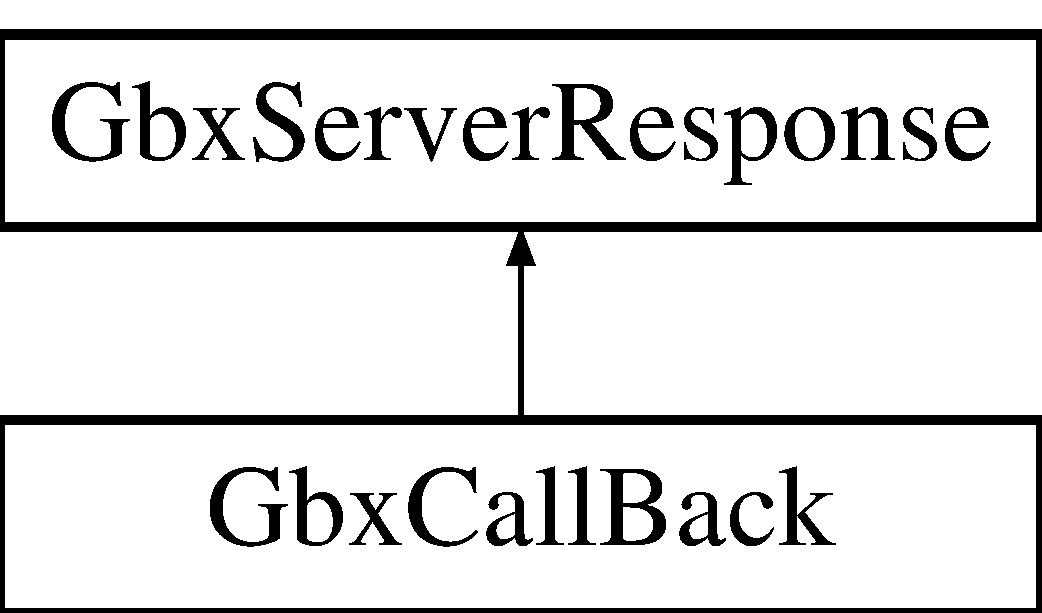
\includegraphics[height=2.000000cm]{classGbxCallBack}
\end{center}
\end{figure}
\subsection*{Public Member Functions}
\begin{DoxyCompactItemize}
\item 
char $\ast$ \hyperlink{classGbxCallBack_a434467d6000e1546e85f94885a816946}{Get\-Method\-Name} ()
\item 
void \hyperlink{classGbxCallBack_a78a993170ce1e3c5a35f02088e4f66a0}{Set\-Raw} (char $\ast$callback)
\begin{DoxyCompactList}\small\item\em Sets the raw message value. \end{DoxyCompactList}\item 
char $\ast$ \hyperlink{classGbxServerResponse_a3105f299a4f6a0d997f909415a467fd5}{Get\-Raw} ()
\begin{DoxyCompactList}\small\item\em Returns raw response (X\-M\-L). \end{DoxyCompactList}\item 
std\-::vector\\*
$<$ \hyperlink{classGbxResponseParameter}{Gbx\-Response\-Parameter} $>$ $\ast$ \hyperlink{classGbxServerResponse_ab791b8d9edb964b909d3c70753549668}{Get\-Parameters} ()
\begin{DoxyCompactList}\small\item\em Returns the extracted parameters. \end{DoxyCompactList}\end{DoxyCompactItemize}
\subsection*{Protected Member Functions}
\begin{DoxyCompactItemize}
\item 
\hyperlink{classGbxResponseParameter}{Gbx\-Response\-Parameter} \hyperlink{classGbxServerResponse_afa89ad0963df83f64934c9a54bb0dac6}{extract\-Param} (tinyxml2\-::\-X\-M\-L\-Element $\ast$param)
\begin{DoxyCompactList}\small\item\em Extracts parameters from the raw data (X\-M\-L). \end{DoxyCompactList}\end{DoxyCompactItemize}
\subsection*{Protected Attributes}
\begin{DoxyCompactItemize}
\item 
char $\ast$ \hyperlink{classGbxServerResponse_aeee1fc539a5881334926e5c6789581bd}{data}
\begin{DoxyCompactList}\small\item\em Raw response data. \end{DoxyCompactList}\item 
std\-::vector\\*
$<$ \hyperlink{classGbxResponseParameter}{Gbx\-Response\-Parameter} $>$ $\ast$ \hyperlink{classGbxServerResponse_ad6fef5319c4da9461f4cd0d72d8b5ee8}{parameters} = new std\-::vector$<$\hyperlink{classGbxResponseParameter}{Gbx\-Response\-Parameter}$>$()
\begin{DoxyCompactList}\small\item\em List of parameters. \end{DoxyCompactList}\end{DoxyCompactItemize}
\subsection*{Private Member Functions}
\begin{DoxyCompactItemize}
\item 
void \hyperlink{classGbxCallBack_a0a9b9db5ebdc8040058b542fb51283d7}{extract\-Parameters} ()
\begin{DoxyCompactList}\small\item\em Extracts parameters from the raw data (X\-M\-L). \end{DoxyCompactList}\end{DoxyCompactItemize}
\subsection*{Private Attributes}
\begin{DoxyCompactItemize}
\item 
char $\ast$ \hyperlink{classGbxCallBack_a767f111fc7851cf31b3bf86dfd816b85}{method\-Name}
\begin{DoxyCompactList}\small\item\em Method name. \end{DoxyCompactList}\end{DoxyCompactItemize}


\subsection{Detailed Description}
Call\-Back from server, de-\/\-X\-M\-L-\/fies the callback. 

\subsection{Member Function Documentation}
\hypertarget{classGbxServerResponse_afa89ad0963df83f64934c9a54bb0dac6}{\index{Gbx\-Call\-Back@{Gbx\-Call\-Back}!extract\-Param@{extract\-Param}}
\index{extract\-Param@{extract\-Param}!GbxCallBack@{Gbx\-Call\-Back}}
\subsubsection[{extract\-Param}]{\setlength{\rightskip}{0pt plus 5cm}{\bf Gbx\-Response\-Parameter} Gbx\-Server\-Response\-::extract\-Param (
\begin{DoxyParamCaption}
\item[{tinyxml2\-::\-X\-M\-L\-Element $\ast$}]{param}
\end{DoxyParamCaption}
)\hspace{0.3cm}{\ttfamily [protected]}, {\ttfamily [inherited]}}}\label{classGbxServerResponse_afa89ad0963df83f64934c9a54bb0dac6}


Extracts parameters from the raw data (X\-M\-L). 

\hypertarget{classGbxCallBack_a0a9b9db5ebdc8040058b542fb51283d7}{\index{Gbx\-Call\-Back@{Gbx\-Call\-Back}!extract\-Parameters@{extract\-Parameters}}
\index{extract\-Parameters@{extract\-Parameters}!GbxCallBack@{Gbx\-Call\-Back}}
\subsubsection[{extract\-Parameters}]{\setlength{\rightskip}{0pt plus 5cm}void Gbx\-Call\-Back\-::extract\-Parameters (
\begin{DoxyParamCaption}
{}
\end{DoxyParamCaption}
)\hspace{0.3cm}{\ttfamily [private]}}}\label{classGbxCallBack_a0a9b9db5ebdc8040058b542fb51283d7}


Extracts parameters from the raw data (X\-M\-L). 

\hypertarget{classGbxCallBack_a434467d6000e1546e85f94885a816946}{\index{Gbx\-Call\-Back@{Gbx\-Call\-Back}!Get\-Method\-Name@{Get\-Method\-Name}}
\index{Get\-Method\-Name@{Get\-Method\-Name}!GbxCallBack@{Gbx\-Call\-Back}}
\subsubsection[{Get\-Method\-Name}]{\setlength{\rightskip}{0pt plus 5cm}char $\ast$ Gbx\-Call\-Back\-::\-Get\-Method\-Name (
\begin{DoxyParamCaption}
{}
\end{DoxyParamCaption}
)}}\label{classGbxCallBack_a434467d6000e1546e85f94885a816946}
Returns the method name. \hypertarget{classGbxServerResponse_ab791b8d9edb964b909d3c70753549668}{\index{Gbx\-Call\-Back@{Gbx\-Call\-Back}!Get\-Parameters@{Get\-Parameters}}
\index{Get\-Parameters@{Get\-Parameters}!GbxCallBack@{Gbx\-Call\-Back}}
\subsubsection[{Get\-Parameters}]{\setlength{\rightskip}{0pt plus 5cm}std\-::vector$<$ {\bf Gbx\-Response\-Parameter} $>$ $\ast$ Gbx\-Server\-Response\-::\-Get\-Parameters (
\begin{DoxyParamCaption}
{}
\end{DoxyParamCaption}
)\hspace{0.3cm}{\ttfamily [inherited]}}}\label{classGbxServerResponse_ab791b8d9edb964b909d3c70753549668}


Returns the extracted parameters. 

\hypertarget{classGbxServerResponse_a3105f299a4f6a0d997f909415a467fd5}{\index{Gbx\-Call\-Back@{Gbx\-Call\-Back}!Get\-Raw@{Get\-Raw}}
\index{Get\-Raw@{Get\-Raw}!GbxCallBack@{Gbx\-Call\-Back}}
\subsubsection[{Get\-Raw}]{\setlength{\rightskip}{0pt plus 5cm}char $\ast$ Gbx\-Server\-Response\-::\-Get\-Raw (
\begin{DoxyParamCaption}
{}
\end{DoxyParamCaption}
)\hspace{0.3cm}{\ttfamily [inherited]}}}\label{classGbxServerResponse_a3105f299a4f6a0d997f909415a467fd5}


Returns raw response (X\-M\-L). 

\hypertarget{classGbxCallBack_a78a993170ce1e3c5a35f02088e4f66a0}{\index{Gbx\-Call\-Back@{Gbx\-Call\-Back}!Set\-Raw@{Set\-Raw}}
\index{Set\-Raw@{Set\-Raw}!GbxCallBack@{Gbx\-Call\-Back}}
\subsubsection[{Set\-Raw}]{\setlength{\rightskip}{0pt plus 5cm}void Gbx\-Call\-Back\-::\-Set\-Raw (
\begin{DoxyParamCaption}
\item[{char $\ast$}]{callback}
\end{DoxyParamCaption}
)}}\label{classGbxCallBack_a78a993170ce1e3c5a35f02088e4f66a0}


Sets the raw message value. 


\begin{DoxyParams}{Parameters}
{\em callback} & Raw callback from server (X\-M\-L). \\
\hline
\end{DoxyParams}


\subsection{Member Data Documentation}
\hypertarget{classGbxServerResponse_aeee1fc539a5881334926e5c6789581bd}{\index{Gbx\-Call\-Back@{Gbx\-Call\-Back}!data@{data}}
\index{data@{data}!GbxCallBack@{Gbx\-Call\-Back}}
\subsubsection[{data}]{\setlength{\rightskip}{0pt plus 5cm}char$\ast$ Gbx\-Server\-Response\-::data\hspace{0.3cm}{\ttfamily [protected]}, {\ttfamily [inherited]}}}\label{classGbxServerResponse_aeee1fc539a5881334926e5c6789581bd}


Raw response data. 

\hypertarget{classGbxCallBack_a767f111fc7851cf31b3bf86dfd816b85}{\index{Gbx\-Call\-Back@{Gbx\-Call\-Back}!method\-Name@{method\-Name}}
\index{method\-Name@{method\-Name}!GbxCallBack@{Gbx\-Call\-Back}}
\subsubsection[{method\-Name}]{\setlength{\rightskip}{0pt plus 5cm}char$\ast$ Gbx\-Call\-Back\-::method\-Name\hspace{0.3cm}{\ttfamily [private]}}}\label{classGbxCallBack_a767f111fc7851cf31b3bf86dfd816b85}


Method name. 

\hypertarget{classGbxServerResponse_ad6fef5319c4da9461f4cd0d72d8b5ee8}{\index{Gbx\-Call\-Back@{Gbx\-Call\-Back}!parameters@{parameters}}
\index{parameters@{parameters}!GbxCallBack@{Gbx\-Call\-Back}}
\subsubsection[{parameters}]{\setlength{\rightskip}{0pt plus 5cm}std\-::vector$<${\bf Gbx\-Response\-Parameter}$>$$\ast$ Gbx\-Server\-Response\-::parameters = new std\-::vector$<${\bf Gbx\-Response\-Parameter}$>$()\hspace{0.3cm}{\ttfamily [protected]}, {\ttfamily [inherited]}}}\label{classGbxServerResponse_ad6fef5319c4da9461f4cd0d72d8b5ee8}


List of parameters. 



The documentation for this class was generated from the following files\-:\begin{DoxyCompactItemize}
\item 
/home/travis/build/\-The\-Maximum/mania-\/pp/src/\-Gbx\-Remote/\-Call\-Back/\hyperlink{GbxCallBack_8h}{Gbx\-Call\-Back.\-h}\item 
/home/travis/build/\-The\-Maximum/mania-\/pp/src/\-Gbx\-Remote/\-Call\-Back/\hyperlink{GbxCallBack_8cpp}{Gbx\-Call\-Back.\-cpp}\end{DoxyCompactItemize}

\hypertarget{structGbxError}{\section{Gbx\-Error Struct Reference}
\label{structGbxError}\index{Gbx\-Error@{Gbx\-Error}}
}


Stores error details from the communication with the server.  




{\ttfamily \#include $<$Gbx\-Structs.\-h$>$}

\subsection*{Public Attributes}
\begin{DoxyCompactItemize}
\item 
int \hyperlink{structGbxError_ae5627cae63e837beaa75f798e47be50e}{number} = 0
\begin{DoxyCompactList}\small\item\em Number of the error (default\-: 0, no error). \end{DoxyCompactList}\item 
std\-::string \hyperlink{structGbxError_af52353692b5c160deac99c4285f01a5a}{message}
\begin{DoxyCompactList}\small\item\em Error message. \end{DoxyCompactList}\end{DoxyCompactItemize}


\subsection{Detailed Description}
Stores error details from the communication with the server. 

\subsection{Member Data Documentation}
\hypertarget{structGbxError_af52353692b5c160deac99c4285f01a5a}{\index{Gbx\-Error@{Gbx\-Error}!message@{message}}
\index{message@{message}!GbxError@{Gbx\-Error}}
\subsubsection[{message}]{\setlength{\rightskip}{0pt plus 5cm}std\-::string Gbx\-Error\-::message}}\label{structGbxError_af52353692b5c160deac99c4285f01a5a}


Error message. 

\hypertarget{structGbxError_ae5627cae63e837beaa75f798e47be50e}{\index{Gbx\-Error@{Gbx\-Error}!number@{number}}
\index{number@{number}!GbxError@{Gbx\-Error}}
\subsubsection[{number}]{\setlength{\rightskip}{0pt plus 5cm}int Gbx\-Error\-::number = 0}}\label{structGbxError_ae5627cae63e837beaa75f798e47be50e}


Number of the error (default\-: 0, no error). 



The documentation for this struct was generated from the following file\-:\begin{DoxyCompactItemize}
\item 
/home/travis/build/\-The\-Maximum/mania-\/pp/src/\-Gbx\-Remote/\hyperlink{GbxStructs_8h}{Gbx\-Structs.\-h}\end{DoxyCompactItemize}

\hypertarget{structGbxFirstResponse}{\section{Gbx\-First\-Response Struct Reference}
\label{structGbxFirstResponse}\index{Gbx\-First\-Response@{Gbx\-First\-Response}}
}


Response received on handshake.  




{\ttfamily \#include $<$Gbx\-Structs.\-h$>$}

\subsection*{Public Attributes}
\begin{DoxyCompactItemize}
\item 
short \hyperlink{structGbxFirstResponse_ad93a9c67024b28ecddb779457dd001f8}{size}
\begin{DoxyCompactList}\small\item\em Size in bytes of the protocol message (usually 11). \end{DoxyCompactList}\end{DoxyCompactItemize}


\subsection{Detailed Description}
Response received on handshake. 

\subsection{Member Data Documentation}
\hypertarget{structGbxFirstResponse_ad93a9c67024b28ecddb779457dd001f8}{\index{Gbx\-First\-Response@{Gbx\-First\-Response}!size@{size}}
\index{size@{size}!GbxFirstResponse@{Gbx\-First\-Response}}
\subsubsection[{size}]{\setlength{\rightskip}{0pt plus 5cm}short Gbx\-First\-Response\-::size}}\label{structGbxFirstResponse_ad93a9c67024b28ecddb779457dd001f8}


Size in bytes of the protocol message (usually 11). 



The documentation for this struct was generated from the following file\-:\begin{DoxyCompactItemize}
\item 
/home/travis/build/\-The\-Maximum/mania-\/pp/src/\-Gbx\-Remote/\hyperlink{GbxStructs_8h}{Gbx\-Structs.\-h}\end{DoxyCompactItemize}

\hypertarget{classGbxMessage}{\section{Gbx\-Message Class Reference}
\label{classGbxMessage}\index{Gbx\-Message@{Gbx\-Message}}
}


X\-M\-L-\/fies the message for communication with the server.  




{\ttfamily \#include $<$Gbx\-Message.\-h$>$}

\subsection*{Public Member Functions}
\begin{DoxyCompactItemize}
\item 
\hyperlink{classGbxMessage_ad4a5e5f75787e12229cf03aabc4ad930}{Gbx\-Message} (std\-::string \hyperlink{classGbxMessage_a10b6118916999db98f28e3f495eef6b4}{method}, \hyperlink{classGbxParameters}{Gbx\-Parameters} $\ast$parameters=N\-U\-L\-L)
\begin{DoxyCompactList}\small\item\em Builds X\-M\-L message. \end{DoxyCompactList}\item 
std\-::string \hyperlink{classGbxMessage_a53e00a162c293251bef476ad74d0134c}{Get\-Method} ()
\begin{DoxyCompactList}\small\item\em Returns the method name. \end{DoxyCompactList}\item 
std\-::string \hyperlink{classGbxMessage_ac81e16efce7da483a696d6653e18c9d8}{Get\-Xml} ()
\begin{DoxyCompactList}\small\item\em Returns the created X\-M\-L message. \end{DoxyCompactList}\end{DoxyCompactItemize}
\subsection*{Private Attributes}
\begin{DoxyCompactItemize}
\item 
std\-::string \hyperlink{classGbxMessage_a10b6118916999db98f28e3f495eef6b4}{method}
\begin{DoxyCompactList}\small\item\em Server method name. \end{DoxyCompactList}\item 
std\-::string \hyperlink{classGbxMessage_a6ea9adbeb3f1c104fa08fce0b1a4090d}{xml}
\begin{DoxyCompactList}\small\item\em Created X\-M\-L message. \end{DoxyCompactList}\end{DoxyCompactItemize}


\subsection{Detailed Description}
X\-M\-L-\/fies the message for communication with the server. 

\subsection{Constructor \& Destructor Documentation}
\hypertarget{classGbxMessage_ad4a5e5f75787e12229cf03aabc4ad930}{\index{Gbx\-Message@{Gbx\-Message}!Gbx\-Message@{Gbx\-Message}}
\index{Gbx\-Message@{Gbx\-Message}!GbxMessage@{Gbx\-Message}}
\subsubsection[{Gbx\-Message}]{\setlength{\rightskip}{0pt plus 5cm}Gbx\-Message\-::\-Gbx\-Message (
\begin{DoxyParamCaption}
\item[{std\-::string}]{method, }
\item[{{\bf Gbx\-Parameters} $\ast$}]{parameters = {\ttfamily NULL}}
\end{DoxyParamCaption}
)}}\label{classGbxMessage_ad4a5e5f75787e12229cf03aabc4ad930}


Builds X\-M\-L message. 


\begin{DoxyParams}{Parameters}
{\em method} & Server method name. \\
\hline
{\em params} & Params which belong to the method. \\
\hline
\end{DoxyParams}


\subsection{Member Function Documentation}
\hypertarget{classGbxMessage_a53e00a162c293251bef476ad74d0134c}{\index{Gbx\-Message@{Gbx\-Message}!Get\-Method@{Get\-Method}}
\index{Get\-Method@{Get\-Method}!GbxMessage@{Gbx\-Message}}
\subsubsection[{Get\-Method}]{\setlength{\rightskip}{0pt plus 5cm}std\-::string Gbx\-Message\-::\-Get\-Method (
\begin{DoxyParamCaption}
{}
\end{DoxyParamCaption}
)}}\label{classGbxMessage_a53e00a162c293251bef476ad74d0134c}


Returns the method name. 

\hypertarget{classGbxMessage_ac81e16efce7da483a696d6653e18c9d8}{\index{Gbx\-Message@{Gbx\-Message}!Get\-Xml@{Get\-Xml}}
\index{Get\-Xml@{Get\-Xml}!GbxMessage@{Gbx\-Message}}
\subsubsection[{Get\-Xml}]{\setlength{\rightskip}{0pt plus 5cm}std\-::string Gbx\-Message\-::\-Get\-Xml (
\begin{DoxyParamCaption}
{}
\end{DoxyParamCaption}
)}}\label{classGbxMessage_ac81e16efce7da483a696d6653e18c9d8}


Returns the created X\-M\-L message. 



\subsection{Member Data Documentation}
\hypertarget{classGbxMessage_a10b6118916999db98f28e3f495eef6b4}{\index{Gbx\-Message@{Gbx\-Message}!method@{method}}
\index{method@{method}!GbxMessage@{Gbx\-Message}}
\subsubsection[{method}]{\setlength{\rightskip}{0pt plus 5cm}std\-::string Gbx\-Message\-::method\hspace{0.3cm}{\ttfamily [private]}}}\label{classGbxMessage_a10b6118916999db98f28e3f495eef6b4}


Server method name. 

\hypertarget{classGbxMessage_a6ea9adbeb3f1c104fa08fce0b1a4090d}{\index{Gbx\-Message@{Gbx\-Message}!xml@{xml}}
\index{xml@{xml}!GbxMessage@{Gbx\-Message}}
\subsubsection[{xml}]{\setlength{\rightskip}{0pt plus 5cm}std\-::string Gbx\-Message\-::xml\hspace{0.3cm}{\ttfamily [private]}}}\label{classGbxMessage_a6ea9adbeb3f1c104fa08fce0b1a4090d}


Created X\-M\-L message. 



The documentation for this class was generated from the following files\-:\begin{DoxyCompactItemize}
\item 
/home/travis/build/\-The\-Maximum/mania-\/pp/src/\-Gbx\-Remote/\hyperlink{GbxMessage_8h}{Gbx\-Message.\-h}\item 
/home/travis/build/\-The\-Maximum/mania-\/pp/src/\-Gbx\-Remote/\hyperlink{GbxMessage_8cpp}{Gbx\-Message.\-cpp}\end{DoxyCompactItemize}

\hypertarget{structGbxParam}{\section{Gbx\-Param Struct Reference}
\label{structGbxParam}\index{Gbx\-Param@{Gbx\-Param}}
}


Pointer and type information of a parameter.  




{\ttfamily \#include $<$Gbx\-Parameters.\-h$>$}

\subsection*{Public Attributes}
\begin{DoxyCompactItemize}
\item 
void $\ast$ \hyperlink{structGbxParam_a19b53f8dacdd8937e1020775f8615495}{pointer}
\begin{DoxyCompactList}\small\item\em Pointer to the parameter. \end{DoxyCompactList}\item 
const std\-::type\-\_\-info $\ast$ \hyperlink{structGbxParam_afb3596a5ba95fda1e27a5c6b4ed517b5}{typeinfo}
\begin{DoxyCompactList}\small\item\em Type information of the parameter. \end{DoxyCompactList}\end{DoxyCompactItemize}


\subsection{Detailed Description}
Pointer and type information of a parameter. 

\subsection{Member Data Documentation}
\hypertarget{structGbxParam_a19b53f8dacdd8937e1020775f8615495}{\index{Gbx\-Param@{Gbx\-Param}!pointer@{pointer}}
\index{pointer@{pointer}!GbxParam@{Gbx\-Param}}
\subsubsection[{pointer}]{\setlength{\rightskip}{0pt plus 5cm}void$\ast$ Gbx\-Param\-::pointer}}\label{structGbxParam_a19b53f8dacdd8937e1020775f8615495}


Pointer to the parameter. 

\hypertarget{structGbxParam_afb3596a5ba95fda1e27a5c6b4ed517b5}{\index{Gbx\-Param@{Gbx\-Param}!typeinfo@{typeinfo}}
\index{typeinfo@{typeinfo}!GbxParam@{Gbx\-Param}}
\subsubsection[{typeinfo}]{\setlength{\rightskip}{0pt plus 5cm}const std\-::type\-\_\-info$\ast$ Gbx\-Param\-::typeinfo}}\label{structGbxParam_afb3596a5ba95fda1e27a5c6b4ed517b5}


Type information of the parameter. 



The documentation for this struct was generated from the following file\-:\begin{DoxyCompactItemize}
\item 
/home/travis/build/\-The\-Maximum/mania-\/pp/src/\-Gbx\-Remote/\-Parameters/\hyperlink{GbxParameters_8h}{Gbx\-Parameters.\-h}\end{DoxyCompactItemize}

\hypertarget{classGbxParameter}{\section{Gbx\-Parameter Class Reference}
\label{classGbxParameter}\index{Gbx\-Parameter@{Gbx\-Parameter}}
}


X\-M\-L-\/fies the parameter for communication with the server.  




{\ttfamily \#include $<$Gbx\-Parameter.\-h$>$}

\subsection*{Public Member Functions}
\begin{DoxyCompactItemize}
\item 
\hyperlink{classGbxParameter_a6cfd5c21c176ca6d9d2a1a3d9ad9953c}{Gbx\-Parameter} (\hyperlink{structGbxParam}{Gbx\-Param} param)
\begin{DoxyCompactList}\small\item\em Casts parameter to string and calls calculate\-Type. \end{DoxyCompactList}\item 
\hypertarget{classGbxParameter_a3c6800bca78c5bb4ed7de62cf552ee35}{std\-::string \hyperlink{classGbxParameter_a3c6800bca78c5bb4ed7de62cf552ee35}{Get\-Xml} ()}\label{classGbxParameter_a3c6800bca78c5bb4ed7de62cf552ee35}

\begin{DoxyCompactList}\small\item\em Returns xml-\/fied parameter. \end{DoxyCompactList}\end{DoxyCompactItemize}
\subsection*{Private Member Functions}
\begin{DoxyCompactItemize}
\item 
void \hyperlink{classGbxParameter_af708857623b85684ede2ae002e53a118}{determine\-Type} (const std\-::type\-\_\-info $\ast$param)
\begin{DoxyCompactList}\small\item\em Determines which X\-M\-L-\/\-R\-P\-C type the parameter has. \end{DoxyCompactList}\item 
void \hyperlink{classGbxParameter_a8e038bca99e1eb7339567fe1af79586c}{dereference\-Data} (void $\ast$param)
\begin{DoxyCompactList}\small\item\em Converts the void pointer into the type determined in determine\-Type. \end{DoxyCompactList}\end{DoxyCompactItemize}
\subsection*{Private Attributes}
\begin{DoxyCompactItemize}
\item 
\hypertarget{classGbxParameter_a6b64cfaae4d5b3b498fb2cdd3d28f824}{std\-::string \hyperlink{classGbxParameter_a6b64cfaae4d5b3b498fb2cdd3d28f824}{data}}\label{classGbxParameter_a6b64cfaae4d5b3b498fb2cdd3d28f824}

\begin{DoxyCompactList}\small\item\em Stringified parameter. \end{DoxyCompactList}\item 
\hypertarget{classGbxParameter_a19d4cab065cb0440c675e97babf45d02}{std\-::string \hyperlink{classGbxParameter_a19d4cab065cb0440c675e97babf45d02}{type}}\label{classGbxParameter_a19d4cab065cb0440c675e97babf45d02}

\begin{DoxyCompactList}\small\item\em Stringified parameter type for X\-M\-L. \end{DoxyCompactList}\item 
\hypertarget{classGbxParameter_ad5182c3df0c77e011c61e00e182f8a49}{std\-::string \hyperlink{classGbxParameter_ad5182c3df0c77e011c61e00e182f8a49}{xml\-Type}}\label{classGbxParameter_ad5182c3df0c77e011c61e00e182f8a49}

\begin{DoxyCompactList}\small\item\em Stringified parameter type for X\-M\-L. \end{DoxyCompactList}\end{DoxyCompactItemize}


\subsection{Detailed Description}
X\-M\-L-\/fies the parameter for communication with the server. 

\subsection{Constructor \& Destructor Documentation}
\hypertarget{classGbxParameter_a6cfd5c21c176ca6d9d2a1a3d9ad9953c}{\index{Gbx\-Parameter@{Gbx\-Parameter}!Gbx\-Parameter@{Gbx\-Parameter}}
\index{Gbx\-Parameter@{Gbx\-Parameter}!GbxParameter@{Gbx\-Parameter}}
\subsubsection[{Gbx\-Parameter}]{\setlength{\rightskip}{0pt plus 5cm}Gbx\-Parameter\-::\-Gbx\-Parameter (
\begin{DoxyParamCaption}
\item[{{\bf Gbx\-Param}}]{param}
\end{DoxyParamCaption}
)}}\label{classGbxParameter_a6cfd5c21c176ca6d9d2a1a3d9ad9953c}


Casts parameter to string and calls calculate\-Type. 


\begin{DoxyParams}{Parameters}
{\em param} & Parameter to be xml-\/fied. \\
\hline
\end{DoxyParams}


\subsection{Member Function Documentation}
\hypertarget{classGbxParameter_a8e038bca99e1eb7339567fe1af79586c}{\index{Gbx\-Parameter@{Gbx\-Parameter}!dereference\-Data@{dereference\-Data}}
\index{dereference\-Data@{dereference\-Data}!GbxParameter@{Gbx\-Parameter}}
\subsubsection[{dereference\-Data}]{\setlength{\rightskip}{0pt plus 5cm}void Gbx\-Parameter\-::dereference\-Data (
\begin{DoxyParamCaption}
\item[{void $\ast$}]{param}
\end{DoxyParamCaption}
)\hspace{0.3cm}{\ttfamily [private]}}}\label{classGbxParameter_a8e038bca99e1eb7339567fe1af79586c}


Converts the void pointer into the type determined in determine\-Type. 


\begin{DoxyParams}{Parameters}
{\em param} & Void pointer to parameter. \\
\hline
\end{DoxyParams}
\hypertarget{classGbxParameter_af708857623b85684ede2ae002e53a118}{\index{Gbx\-Parameter@{Gbx\-Parameter}!determine\-Type@{determine\-Type}}
\index{determine\-Type@{determine\-Type}!GbxParameter@{Gbx\-Parameter}}
\subsubsection[{determine\-Type}]{\setlength{\rightskip}{0pt plus 5cm}void Gbx\-Parameter\-::determine\-Type (
\begin{DoxyParamCaption}
\item[{const std\-::type\-\_\-info $\ast$}]{param}
\end{DoxyParamCaption}
)\hspace{0.3cm}{\ttfamily [private]}}}\label{classGbxParameter_af708857623b85684ede2ae002e53a118}


Determines which X\-M\-L-\/\-R\-P\-C type the parameter has. 


\begin{DoxyParams}{Parameters}
{\em param} & Type information about the parameter. \\
\hline
\end{DoxyParams}


The documentation for this class was generated from the following files\-:\begin{DoxyCompactItemize}
\item 
/home/travis/build/\-The\-Maximum/mania-\/pp/src/\-Gbx\-Remote/\-Parameters/Gbx\-Parameter.\-h\item 
/home/travis/build/\-The\-Maximum/mania-\/pp/src/\-Gbx\-Remote/\-Parameters/Gbx\-Parameter.\-cpp\end{DoxyCompactItemize}

\hypertarget{classGbxParameters}{\section{Gbx\-Parameters Class Reference}
\label{classGbxParameters}\index{Gbx\-Parameters@{Gbx\-Parameters}}
}


List of parameters.  




{\ttfamily \#include $<$Gbx\-Parameters.\-h$>$}

\subsection*{Public Member Functions}
\begin{DoxyCompactItemize}
\item 
{\footnotesize template$<$typename T $>$ }\\void \hyperlink{classGbxParameters_a2cf83794717cf9fdc13e5ff12e259f04}{Put} (T $\ast$pointer)
\begin{DoxyCompactList}\small\item\em Add parameter to the list. \end{DoxyCompactList}\item 
\hypertarget{classGbxParameters_a09302bc40359205cd294b8bcf2ab1c2e}{std\-::vector$<$ \hyperlink{structGbxParam}{Gbx\-Param} $>$ \hyperlink{classGbxParameters_a09302bc40359205cd294b8bcf2ab1c2e}{Get\-Parameters} ()}\label{classGbxParameters_a09302bc40359205cd294b8bcf2ab1c2e}

\begin{DoxyCompactList}\small\item\em Return the current list of parameters. \end{DoxyCompactList}\end{DoxyCompactItemize}
\subsection*{Private Attributes}
\begin{DoxyCompactItemize}
\item 
\hypertarget{classGbxParameters_aeabcb21396d3198d718c94de23595750}{std\-::vector$<$ \hyperlink{structGbxParam}{Gbx\-Param} $>$ \hyperlink{classGbxParameters_aeabcb21396d3198d718c94de23595750}{parameters} = std\-::vector$<$\hyperlink{structGbxParam}{Gbx\-Param}$>$()}\label{classGbxParameters_aeabcb21396d3198d718c94de23595750}

\begin{DoxyCompactList}\small\item\em List of parameters. \end{DoxyCompactList}\end{DoxyCompactItemize}


\subsection{Detailed Description}
List of parameters. 

\subsection{Member Function Documentation}
\hypertarget{classGbxParameters_a2cf83794717cf9fdc13e5ff12e259f04}{\index{Gbx\-Parameters@{Gbx\-Parameters}!Put@{Put}}
\index{Put@{Put}!GbxParameters@{Gbx\-Parameters}}
\subsubsection[{Put}]{\setlength{\rightskip}{0pt plus 5cm}template$<$typename T $>$ void Gbx\-Parameters\-::\-Put (
\begin{DoxyParamCaption}
\item[{T $\ast$}]{pointer}
\end{DoxyParamCaption}
)\hspace{0.3cm}{\ttfamily [inline]}}}\label{classGbxParameters_a2cf83794717cf9fdc13e5ff12e259f04}


Add parameter to the list. 


\begin{DoxyParams}{Parameters}
{\em pointer} & Pointer to the parameter. \\
\hline
\end{DoxyParams}


The documentation for this class was generated from the following file\-:\begin{DoxyCompactItemize}
\item 
/home/travis/build/\-The\-Maximum/mania-\/pp/src/\-Gbx\-Remote/\-Parameters/Gbx\-Parameters.\-h\end{DoxyCompactItemize}

\hypertarget{structGbxQueryResponse}{\section{Gbx\-Query\-Response Struct Reference}
\label{structGbxQueryResponse}\index{Gbx\-Query\-Response@{Gbx\-Query\-Response}}
}


Response received after a query is sent.  




{\ttfamily \#include $<$Gbx\-Structs.\-h$>$}

\subsection*{Public Attributes}
\begin{DoxyCompactItemize}
\item 
short \hyperlink{structGbxQueryResponse_ab7d7e30d6beb443cdae8cbf95e4c89f3}{size}
\begin{DoxyCompactList}\small\item\em Size in bytes of the query response. \end{DoxyCompactList}\item 
long \hyperlink{structGbxQueryResponse_ad37f7d084a89880263a2a36287427af3}{handle}
\begin{DoxyCompactList}\small\item\em Handle identifier of response message. \end{DoxyCompactList}\end{DoxyCompactItemize}


\subsection{Detailed Description}
Response received after a query is sent. 

\subsection{Member Data Documentation}
\hypertarget{structGbxQueryResponse_ad37f7d084a89880263a2a36287427af3}{\index{Gbx\-Query\-Response@{Gbx\-Query\-Response}!handle@{handle}}
\index{handle@{handle}!GbxQueryResponse@{Gbx\-Query\-Response}}
\subsubsection[{handle}]{\setlength{\rightskip}{0pt plus 5cm}long Gbx\-Query\-Response\-::handle}}\label{structGbxQueryResponse_ad37f7d084a89880263a2a36287427af3}


Handle identifier of response message. 

\hypertarget{structGbxQueryResponse_ab7d7e30d6beb443cdae8cbf95e4c89f3}{\index{Gbx\-Query\-Response@{Gbx\-Query\-Response}!size@{size}}
\index{size@{size}!GbxQueryResponse@{Gbx\-Query\-Response}}
\subsubsection[{size}]{\setlength{\rightskip}{0pt plus 5cm}short Gbx\-Query\-Response\-::size}}\label{structGbxQueryResponse_ab7d7e30d6beb443cdae8cbf95e4c89f3}


Size in bytes of the query response. 



The documentation for this struct was generated from the following file\-:\begin{DoxyCompactItemize}
\item 
/home/travis/build/\-The\-Maximum/mania-\/pp/src/\-Gbx\-Remote/\hyperlink{GbxStructs_8h}{Gbx\-Structs.\-h}\end{DoxyCompactItemize}

\hypertarget{classGbxRemote}{\section{Gbx\-Remote Class Reference}
\label{classGbxRemote}\index{Gbx\-Remote@{Gbx\-Remote}}
}


Handles communication with the Mania\-Planet server.  




{\ttfamily \#include $<$Gbx\-Remote.\-h$>$}

\subsection*{Public Member Functions}
\begin{DoxyCompactItemize}
\item 
\hyperlink{classGbxRemote_a9ac65a51eb6f9127337b4f99841cfe2d}{$\sim$\-Gbx\-Remote} ()
\item 
bool \hyperlink{classGbxRemote_a24d9d0df923ed85010f53dcb43c2b977}{Init} (int port)
\begin{DoxyCompactList}\small\item\em Initializes connection with the local server. \end{DoxyCompactList}\item 
bool \hyperlink{classGbxRemote_aa9a57e73f2f5ebbde90484503bd0d16d}{Init\-With\-Ip} (std\-::string address, int port)
\begin{DoxyCompactList}\small\item\em Initializes connection with the server. \end{DoxyCompactList}\item 
\hypertarget{classGbxRemote_a6fa8ca2d48aae84884cab98a0adf4360}{void \hyperlink{classGbxRemote_a6fa8ca2d48aae84884cab98a0adf4360}{Terminate} ()}\label{classGbxRemote_a6fa8ca2d48aae84884cab98a0adf4360}

\begin{DoxyCompactList}\small\item\em Closes the connection with the server. \end{DoxyCompactList}\item 
bool \hyperlink{classGbxRemote_a8ecc0e0625a8dca310cebd78bd2b3c7e}{Query} (\hyperlink{classGbxMessage}{Gbx\-Message} query)
\begin{DoxyCompactList}\small\item\em Sends a \hyperlink{classGbxMessage}{Gbx\-Message} to the server. \end{DoxyCompactList}\item 
bool \hyperlink{classGbxRemote_ac595861af2f4d7349ce3841f0758507d}{Read\-Call\-Backs} ()
\begin{DoxyCompactList}\small\item\em Read callbacks from the server. \end{DoxyCompactList}\item 
void \hyperlink{classGbxRemote_a5bd6e1dc2118f7e369e72592b3c9322a}{Handle\-Call\-Back} (std\-::string data)
\begin{DoxyCompactList}\small\item\em Handles callbacks (de-\/\-X\-M\-L-\/fies them). \end{DoxyCompactList}\item 
\hypertarget{classGbxRemote_a1ae6ff7eddcccdeda59af2316d053aae}{std\-::vector$<$ \hyperlink{classGbxCallBack}{Gbx\-Call\-Back} $>$ \hyperlink{classGbxRemote_a1ae6ff7eddcccdeda59af2316d053aae}{Get\-C\-B\-Responses} ()}\label{classGbxRemote_a1ae6ff7eddcccdeda59af2316d053aae}

\begin{DoxyCompactList}\small\item\em Returns the callbacks that have been received since last call. \end{DoxyCompactList}\item 
\hypertarget{classGbxRemote_a81ba62f042948610a3cf720316e22076}{void \hyperlink{classGbxRemote_a81ba62f042948610a3cf720316e22076}{Reset\-C\-B\-Responses} ()}\label{classGbxRemote_a81ba62f042948610a3cf720316e22076}

\begin{DoxyCompactList}\small\item\em Resets list of current callbacks. \end{DoxyCompactList}\item 
\hypertarget{classGbxRemote_adac67444e391ffcc1dfda8f087eaef0b}{\hyperlink{classGbxResponse}{Gbx\-Response} $\ast$ \hyperlink{classGbxRemote_adac67444e391ffcc1dfda8f087eaef0b}{Get\-Response} ()}\label{classGbxRemote_adac67444e391ffcc1dfda8f087eaef0b}

\begin{DoxyCompactList}\small\item\em Returns the response from the server. \end{DoxyCompactList}\item 
\hyperlink{structGbxError}{Gbx\-Error} \hyperlink{classGbxRemote_aa3f6e467372a23c3a53510d5488bea8a}{Get\-Current\-Error} ()
\begin{DoxyCompactList}\small\item\em Returns the current server error. \end{DoxyCompactList}\item 
\hypertarget{classGbxRemote_ae6e15060920a31482fd14045cfd42803}{int \hyperlink{classGbxRemote_ae6e15060920a31482fd14045cfd42803}{Get\-Protocol} ()}\label{classGbxRemote_ae6e15060920a31482fd14045cfd42803}

\begin{DoxyCompactList}\small\item\em Returns the current version number of the server protocol (1 or 2). \end{DoxyCompactList}\item 
\hypertarget{classGbxRemote_a6351f71fe649bff2aabfbd9b7c89e3f5}{std\-::string \hyperlink{classGbxRemote_a6351f71fe649bff2aabfbd9b7c89e3f5}{Get\-Api\-Version} ()}\label{classGbxRemote_a6351f71fe649bff2aabfbd9b7c89e3f5}

\begin{DoxyCompactList}\small\item\em Returns the set A\-P\-I version. \end{DoxyCompactList}\end{DoxyCompactItemize}
\subsection*{Private Attributes}
\begin{DoxyCompactItemize}
\item 
\hypertarget{classGbxRemote_a56662ea222345c645ae897e056b5c8c8}{bool \hyperlink{classGbxRemote_a56662ea222345c645ae897e056b5c8c8}{connected} = false}\label{classGbxRemote_a56662ea222345c645ae897e056b5c8c8}

\begin{DoxyCompactList}\small\item\em Is the client connected with the server? \end{DoxyCompactList}\item 
\hypertarget{classGbxRemote_a5ee5c7087085cb6cb2e7bc6135ff0646}{int \hyperlink{classGbxRemote_a5ee5c7087085cb6cb2e7bc6135ff0646}{protocol} = 0}\label{classGbxRemote_a5ee5c7087085cb6cb2e7bc6135ff0646}

\begin{DoxyCompactList}\small\item\em Protocol version (0 = uninitialized, 1 or 2 = version). \end{DoxyCompactList}\item 
\hypertarget{classGbxRemote_a81d3c0c70ab7f5e585840e9978ee900e}{std\-::string \hyperlink{classGbxRemote_a81d3c0c70ab7f5e585840e9978ee900e}{api\-Version}}\label{classGbxRemote_a81d3c0c70ab7f5e585840e9978ee900e}

\begin{DoxyCompactList}\small\item\em Server A\-P\-I version. \end{DoxyCompactList}\item 
\hypertarget{classGbxRemote_a0b0b212b945da4266fb645affdac81cb}{\hyperlink{classTcpClient}{Tcp\-Client} \hyperlink{classGbxRemote_a0b0b212b945da4266fb645affdac81cb}{server}}\label{classGbxRemote_a0b0b212b945da4266fb645affdac81cb}

\begin{DoxyCompactList}\small\item\em Socket connection with the server. \end{DoxyCompactList}\item 
\hypertarget{classGbxRemote_a5c310edc409e31aa12c0c0664b0fd238}{\hyperlink{structGbxError}{Gbx\-Error} \hyperlink{classGbxRemote_a5c310edc409e31aa12c0c0664b0fd238}{current\-Error} = \hyperlink{structGbxError}{Gbx\-Error}()}\label{classGbxRemote_a5c310edc409e31aa12c0c0664b0fd238}

\begin{DoxyCompactList}\small\item\em Current server error. \end{DoxyCompactList}\item 
\hypertarget{classGbxRemote_a3a3a0af1a692a801a33baa292b877dc2}{\hyperlink{classGbxResponse}{Gbx\-Response} $\ast$ \hyperlink{classGbxRemote_a3a3a0af1a692a801a33baa292b877dc2}{current\-Response} = new \hyperlink{classGbxResponse}{Gbx\-Response}}\label{classGbxRemote_a3a3a0af1a692a801a33baa292b877dc2}

\begin{DoxyCompactList}\small\item\em Current server response. \end{DoxyCompactList}\item 
\hypertarget{classGbxRemote_a08d047d7e0d4b746fc036c1aa02f0d17}{std\-::vector$<$ \hyperlink{classGbxCallBack}{Gbx\-Call\-Back} $>$ \hyperlink{classGbxRemote_a08d047d7e0d4b746fc036c1aa02f0d17}{current\-Call\-Backs} = std\-::vector$<$\hyperlink{classGbxCallBack}{Gbx\-Call\-Back}$>$()}\label{classGbxRemote_a08d047d7e0d4b746fc036c1aa02f0d17}

\begin{DoxyCompactList}\small\item\em List of currently received callbacks. \end{DoxyCompactList}\end{DoxyCompactItemize}


\subsection{Detailed Description}
Handles communication with the Mania\-Planet server. 

\begin{DoxyRefDesc}{Todo}
\item[\hyperlink{todo__todo000002}{Todo}]Make it possible to set an A\-P\-I version without upsetting Tiny\-X\-M\-L2. \end{DoxyRefDesc}


\subsection{Constructor \& Destructor Documentation}
\hypertarget{classGbxRemote_a9ac65a51eb6f9127337b4f99841cfe2d}{\index{Gbx\-Remote@{Gbx\-Remote}!$\sim$\-Gbx\-Remote@{$\sim$\-Gbx\-Remote}}
\index{$\sim$\-Gbx\-Remote@{$\sim$\-Gbx\-Remote}!GbxRemote@{Gbx\-Remote}}
\subsubsection[{$\sim$\-Gbx\-Remote}]{\setlength{\rightskip}{0pt plus 5cm}Gbx\-Remote\-::$\sim$\-Gbx\-Remote (
\begin{DoxyParamCaption}
{}
\end{DoxyParamCaption}
)}}\label{classGbxRemote_a9ac65a51eb6f9127337b4f99841cfe2d}
Deletes and nullifies the current\-Error and current\-Response. 

\subsection{Member Function Documentation}
\hypertarget{classGbxRemote_aa3f6e467372a23c3a53510d5488bea8a}{\index{Gbx\-Remote@{Gbx\-Remote}!Get\-Current\-Error@{Get\-Current\-Error}}
\index{Get\-Current\-Error@{Get\-Current\-Error}!GbxRemote@{Gbx\-Remote}}
\subsubsection[{Get\-Current\-Error}]{\setlength{\rightskip}{0pt plus 5cm}{\bf Gbx\-Error} Gbx\-Remote\-::\-Get\-Current\-Error (
\begin{DoxyParamCaption}
{}
\end{DoxyParamCaption}
)}}\label{classGbxRemote_aa3f6e467372a23c3a53510d5488bea8a}


Returns the current server error. 

Returns empty \hyperlink{structGbxError}{Gbx\-Error} when there currently is no error. \hypertarget{classGbxRemote_a5bd6e1dc2118f7e369e72592b3c9322a}{\index{Gbx\-Remote@{Gbx\-Remote}!Handle\-Call\-Back@{Handle\-Call\-Back}}
\index{Handle\-Call\-Back@{Handle\-Call\-Back}!GbxRemote@{Gbx\-Remote}}
\subsubsection[{Handle\-Call\-Back}]{\setlength{\rightskip}{0pt plus 5cm}void Gbx\-Remote\-::\-Handle\-Call\-Back (
\begin{DoxyParamCaption}
\item[{std\-::string}]{data}
\end{DoxyParamCaption}
)}}\label{classGbxRemote_a5bd6e1dc2118f7e369e72592b3c9322a}


Handles callbacks (de-\/\-X\-M\-L-\/fies them). 


\begin{DoxyParams}{Parameters}
{\em data} & Raw response from the server. \\
\hline
\end{DoxyParams}
\hypertarget{classGbxRemote_a24d9d0df923ed85010f53dcb43c2b977}{\index{Gbx\-Remote@{Gbx\-Remote}!Init@{Init}}
\index{Init@{Init}!GbxRemote@{Gbx\-Remote}}
\subsubsection[{Init}]{\setlength{\rightskip}{0pt plus 5cm}bool Gbx\-Remote\-::\-Init (
\begin{DoxyParamCaption}
\item[{int}]{port}
\end{DoxyParamCaption}
)}}\label{classGbxRemote_a24d9d0df923ed85010f53dcb43c2b977}


Initializes connection with the local server. 


\begin{DoxyParams}{Parameters}
{\em port} & X\-M\-L-\/\-R\-P\-C port of the server. \\
\hline
\end{DoxyParams}
\hypertarget{classGbxRemote_aa9a57e73f2f5ebbde90484503bd0d16d}{\index{Gbx\-Remote@{Gbx\-Remote}!Init\-With\-Ip@{Init\-With\-Ip}}
\index{Init\-With\-Ip@{Init\-With\-Ip}!GbxRemote@{Gbx\-Remote}}
\subsubsection[{Init\-With\-Ip}]{\setlength{\rightskip}{0pt plus 5cm}bool Gbx\-Remote\-::\-Init\-With\-Ip (
\begin{DoxyParamCaption}
\item[{std\-::string}]{address, }
\item[{int}]{port}
\end{DoxyParamCaption}
)}}\label{classGbxRemote_aa9a57e73f2f5ebbde90484503bd0d16d}


Initializes connection with the server. 


\begin{DoxyParams}{Parameters}
{\em address} & Address of the server. \\
\hline
{\em port} & X\-M\-L-\/\-R\-P\-C port of the server. \\
\hline
\end{DoxyParams}
\hypertarget{classGbxRemote_a8ecc0e0625a8dca310cebd78bd2b3c7e}{\index{Gbx\-Remote@{Gbx\-Remote}!Query@{Query}}
\index{Query@{Query}!GbxRemote@{Gbx\-Remote}}
\subsubsection[{Query}]{\setlength{\rightskip}{0pt plus 5cm}bool Gbx\-Remote\-::\-Query (
\begin{DoxyParamCaption}
\item[{{\bf Gbx\-Message}}]{query}
\end{DoxyParamCaption}
)}}\label{classGbxRemote_a8ecc0e0625a8dca310cebd78bd2b3c7e}


Sends a \hyperlink{classGbxMessage}{Gbx\-Message} to the server. 

Returns whether the query was successfully sent.


\begin{DoxyParams}{Parameters}
{\em query} & Query to be send. \\
\hline
\end{DoxyParams}
\hypertarget{classGbxRemote_ac595861af2f4d7349ce3841f0758507d}{\index{Gbx\-Remote@{Gbx\-Remote}!Read\-Call\-Backs@{Read\-Call\-Backs}}
\index{Read\-Call\-Backs@{Read\-Call\-Backs}!GbxRemote@{Gbx\-Remote}}
\subsubsection[{Read\-Call\-Backs}]{\setlength{\rightskip}{0pt plus 5cm}bool Gbx\-Remote\-::\-Read\-Call\-Backs (
\begin{DoxyParamCaption}
{}
\end{DoxyParamCaption}
)}}\label{classGbxRemote_ac595861af2f4d7349ce3841f0758507d}


Read callbacks from the server. 

Returns whether it found a callback. 

The documentation for this class was generated from the following files\-:\begin{DoxyCompactItemize}
\item 
/home/travis/build/\-The\-Maximum/mania-\/pp/src/\-Gbx\-Remote/Gbx\-Remote.\-h\item 
/home/travis/build/\-The\-Maximum/mania-\/pp/src/\-Gbx\-Remote/Gbx\-Remote.\-cpp\end{DoxyCompactItemize}

\hypertarget{classGbxResponse}{\section{Gbx\-Response Class Reference}
\label{classGbxResponse}\index{Gbx\-Response@{Gbx\-Response}}
}


Response from server, de-\/\-X\-M\-L-\/fies the response.  




{\ttfamily \#include $<$Gbx\-Response.\-h$>$}

\subsection*{Public Member Functions}
\begin{DoxyCompactItemize}
\item 
\hyperlink{classGbxResponse_ae29114aa0014ca50f3be6455bda1be47}{Gbx\-Response} ()
\begin{DoxyCompactList}\small\item\em Empty constructor. \end{DoxyCompactList}\item 
\hyperlink{classGbxResponse_a27e6c9c3452f2a0c90a33177af84236b}{$\sim$\-Gbx\-Response} ()
\item 
void \hyperlink{classGbxResponse_aadd25f4d4c454bb837af9b442742ff70}{Set\-Raw} (char $\ast$response)
\begin{DoxyCompactList}\small\item\em Sets the raw message value. \end{DoxyCompactList}\item 
char $\ast$ \hyperlink{classGbxResponse_a3311b30d7e04c2a14eb5f675ad6e37cd}{Get\-Raw} ()
\begin{DoxyCompactList}\small\item\em Returns raw response (X\-M\-L). \end{DoxyCompactList}\item 
std\-::vector\\*
$<$ \hyperlink{classGbxResponseParameter}{Gbx\-Response\-Parameter} $>$ $\ast$ \hyperlink{classGbxResponse_a9323a43f94e895422a7ee29a1eb80cc3}{Get\-Parameters} ()
\begin{DoxyCompactList}\small\item\em Returns the extracted parameters. \end{DoxyCompactList}\end{DoxyCompactItemize}
\subsection*{Private Member Functions}
\begin{DoxyCompactItemize}
\item 
void \hyperlink{classGbxResponse_a3cd4d6c5458fcd5359b8f5d9921a2a9b}{extract\-Parameters} ()
\begin{DoxyCompactList}\small\item\em Extracts parameters from the raw data (X\-M\-L). \end{DoxyCompactList}\item 
\hyperlink{classGbxResponseParameter}{Gbx\-Response\-Parameter} \hyperlink{classGbxResponse_af8501950f3b82ce74924f3bda746871b}{extract\-Param} (tinyxml2\-::\-X\-M\-L\-Element $\ast$param)
\begin{DoxyCompactList}\small\item\em Extracts parameters from the raw data (X\-M\-L). \end{DoxyCompactList}\end{DoxyCompactItemize}
\subsection*{Private Attributes}
\begin{DoxyCompactItemize}
\item 
char $\ast$ \hyperlink{classGbxResponse_aee1c7b03d870c87883bd97740afd7675}{data}
\begin{DoxyCompactList}\small\item\em Raw response data. \end{DoxyCompactList}\item 
std\-::vector\\*
$<$ \hyperlink{classGbxResponseParameter}{Gbx\-Response\-Parameter} $>$ $\ast$ \hyperlink{classGbxResponse_afcbec4555fa682d9d1360ecff829d0f2}{parameters} = new std\-::vector$<$\hyperlink{classGbxResponseParameter}{Gbx\-Response\-Parameter}$>$()
\begin{DoxyCompactList}\small\item\em List of parameters. \end{DoxyCompactList}\end{DoxyCompactItemize}


\subsection{Detailed Description}
Response from server, de-\/\-X\-M\-L-\/fies the response. 

\subsection{Constructor \& Destructor Documentation}
\hypertarget{classGbxResponse_ae29114aa0014ca50f3be6455bda1be47}{\index{Gbx\-Response@{Gbx\-Response}!Gbx\-Response@{Gbx\-Response}}
\index{Gbx\-Response@{Gbx\-Response}!GbxResponse@{Gbx\-Response}}
\subsubsection[{Gbx\-Response}]{\setlength{\rightskip}{0pt plus 5cm}Gbx\-Response\-::\-Gbx\-Response (
\begin{DoxyParamCaption}
{}
\end{DoxyParamCaption}
)}}\label{classGbxResponse_ae29114aa0014ca50f3be6455bda1be47}


Empty constructor. 

\hypertarget{classGbxResponse_a27e6c9c3452f2a0c90a33177af84236b}{\index{Gbx\-Response@{Gbx\-Response}!$\sim$\-Gbx\-Response@{$\sim$\-Gbx\-Response}}
\index{$\sim$\-Gbx\-Response@{$\sim$\-Gbx\-Response}!GbxResponse@{Gbx\-Response}}
\subsubsection[{$\sim$\-Gbx\-Response}]{\setlength{\rightskip}{0pt plus 5cm}Gbx\-Response\-::$\sim$\-Gbx\-Response (
\begin{DoxyParamCaption}
{}
\end{DoxyParamCaption}
)}}\label{classGbxResponse_a27e6c9c3452f2a0c90a33177af84236b}
Delets and nullifies the parameters. 

\subsection{Member Function Documentation}
\hypertarget{classGbxResponse_af8501950f3b82ce74924f3bda746871b}{\index{Gbx\-Response@{Gbx\-Response}!extract\-Param@{extract\-Param}}
\index{extract\-Param@{extract\-Param}!GbxResponse@{Gbx\-Response}}
\subsubsection[{extract\-Param}]{\setlength{\rightskip}{0pt plus 5cm}{\bf Gbx\-Response\-Parameter} Gbx\-Response\-::extract\-Param (
\begin{DoxyParamCaption}
\item[{tinyxml2\-::\-X\-M\-L\-Element $\ast$}]{param}
\end{DoxyParamCaption}
)\hspace{0.3cm}{\ttfamily [private]}}}\label{classGbxResponse_af8501950f3b82ce74924f3bda746871b}


Extracts parameters from the raw data (X\-M\-L). 

\hypertarget{classGbxResponse_a3cd4d6c5458fcd5359b8f5d9921a2a9b}{\index{Gbx\-Response@{Gbx\-Response}!extract\-Parameters@{extract\-Parameters}}
\index{extract\-Parameters@{extract\-Parameters}!GbxResponse@{Gbx\-Response}}
\subsubsection[{extract\-Parameters}]{\setlength{\rightskip}{0pt plus 5cm}void Gbx\-Response\-::extract\-Parameters (
\begin{DoxyParamCaption}
{}
\end{DoxyParamCaption}
)\hspace{0.3cm}{\ttfamily [private]}}}\label{classGbxResponse_a3cd4d6c5458fcd5359b8f5d9921a2a9b}


Extracts parameters from the raw data (X\-M\-L). 

\begin{DoxyRefDesc}{Todo}
\item[\hyperlink{todo__todo000001}{Todo}]Add support for structs. \end{DoxyRefDesc}
\hypertarget{classGbxResponse_a9323a43f94e895422a7ee29a1eb80cc3}{\index{Gbx\-Response@{Gbx\-Response}!Get\-Parameters@{Get\-Parameters}}
\index{Get\-Parameters@{Get\-Parameters}!GbxResponse@{Gbx\-Response}}
\subsubsection[{Get\-Parameters}]{\setlength{\rightskip}{0pt plus 5cm}std\-::vector$<$ {\bf Gbx\-Response\-Parameter} $>$ $\ast$ Gbx\-Response\-::\-Get\-Parameters (
\begin{DoxyParamCaption}
{}
\end{DoxyParamCaption}
)}}\label{classGbxResponse_a9323a43f94e895422a7ee29a1eb80cc3}


Returns the extracted parameters. 

\hypertarget{classGbxResponse_a3311b30d7e04c2a14eb5f675ad6e37cd}{\index{Gbx\-Response@{Gbx\-Response}!Get\-Raw@{Get\-Raw}}
\index{Get\-Raw@{Get\-Raw}!GbxResponse@{Gbx\-Response}}
\subsubsection[{Get\-Raw}]{\setlength{\rightskip}{0pt plus 5cm}char $\ast$ Gbx\-Response\-::\-Get\-Raw (
\begin{DoxyParamCaption}
{}
\end{DoxyParamCaption}
)}}\label{classGbxResponse_a3311b30d7e04c2a14eb5f675ad6e37cd}


Returns raw response (X\-M\-L). 

\hypertarget{classGbxResponse_aadd25f4d4c454bb837af9b442742ff70}{\index{Gbx\-Response@{Gbx\-Response}!Set\-Raw@{Set\-Raw}}
\index{Set\-Raw@{Set\-Raw}!GbxResponse@{Gbx\-Response}}
\subsubsection[{Set\-Raw}]{\setlength{\rightskip}{0pt plus 5cm}void Gbx\-Response\-::\-Set\-Raw (
\begin{DoxyParamCaption}
\item[{char $\ast$}]{response}
\end{DoxyParamCaption}
)}}\label{classGbxResponse_aadd25f4d4c454bb837af9b442742ff70}


Sets the raw message value. 


\begin{DoxyParams}{Parameters}
{\em response} & Raw response from server (X\-M\-L). \\
\hline
\end{DoxyParams}


\subsection{Member Data Documentation}
\hypertarget{classGbxResponse_aee1c7b03d870c87883bd97740afd7675}{\index{Gbx\-Response@{Gbx\-Response}!data@{data}}
\index{data@{data}!GbxResponse@{Gbx\-Response}}
\subsubsection[{data}]{\setlength{\rightskip}{0pt plus 5cm}char$\ast$ Gbx\-Response\-::data\hspace{0.3cm}{\ttfamily [private]}}}\label{classGbxResponse_aee1c7b03d870c87883bd97740afd7675}


Raw response data. 

\hypertarget{classGbxResponse_afcbec4555fa682d9d1360ecff829d0f2}{\index{Gbx\-Response@{Gbx\-Response}!parameters@{parameters}}
\index{parameters@{parameters}!GbxResponse@{Gbx\-Response}}
\subsubsection[{parameters}]{\setlength{\rightskip}{0pt plus 5cm}std\-::vector$<${\bf Gbx\-Response\-Parameter}$>$$\ast$ Gbx\-Response\-::parameters = new std\-::vector$<${\bf Gbx\-Response\-Parameter}$>$()\hspace{0.3cm}{\ttfamily [private]}}}\label{classGbxResponse_afcbec4555fa682d9d1360ecff829d0f2}


List of parameters. 



The documentation for this class was generated from the following files\-:\begin{DoxyCompactItemize}
\item 
/home/travis/build/\-The\-Maximum/mania-\/pp/src/\-Gbx\-Remote/\hyperlink{GbxResponse_8h}{Gbx\-Response.\-h}\item 
/home/travis/build/\-The\-Maximum/mania-\/pp/src/\-Gbx\-Remote/\hyperlink{GbxResponse_8cpp}{Gbx\-Response.\-cpp}\end{DoxyCompactItemize}

\hypertarget{classGbxResponseParameter}{\section{Gbx\-Response\-Parameter Class Reference}
\label{classGbxResponseParameter}\index{Gbx\-Response\-Parameter@{Gbx\-Response\-Parameter}}
}


Parameter deducted from server response.  




{\ttfamily \#include $<$Gbx\-Server\-Response.\-h$>$}

\subsection*{Public Member Functions}
\begin{DoxyCompactItemize}
\item 
std\-::vector$<$ \hyperlink{classGbxResponseParameter}{Gbx\-Response\-Parameter} $>$ \hyperlink{classGbxResponseParameter_aa27aca1d5084755fe585401617e2549a}{Get\-Array} ()
\begin{DoxyCompactList}\small\item\em Gets the value as vector of parameters. \end{DoxyCompactList}\item 
std\-::map$<$ std\-::string, \\*
\hyperlink{classGbxResponseParameter}{Gbx\-Response\-Parameter} $>$ \hyperlink{classGbxResponseParameter_ab6af5e0662d7d832b7606e9e0f461f22}{Get\-Struct} ()
\begin{DoxyCompactList}\small\item\em Gets the value as map of parameters. \end{DoxyCompactList}\item 
std\-::string \hyperlink{classGbxResponseParameter_a014af0f74e937d9002cda3e6e791735b}{Get\-String} ()
\begin{DoxyCompactList}\small\item\em Gets the value as string. \end{DoxyCompactList}\end{DoxyCompactItemize}
\subsection*{Public Attributes}
\begin{DoxyCompactItemize}
\item 
std\-::string \hyperlink{classGbxResponseParameter_aa1700ca65fa2526b112be24b5c0bdbf4}{Type}
\begin{DoxyCompactList}\small\item\em X\-M\-L-\/\-R\-P\-C data type. \end{DoxyCompactList}\item 
std\-::vector$<$ \hyperlink{classGbxResponseParameter}{Gbx\-Response\-Parameter} $>$ \hyperlink{classGbxResponseParameter_abd56daae71edf6749b634d0545a85aad}{Array}
\begin{DoxyCompactList}\small\item\em Parameters as array. \end{DoxyCompactList}\item 
std\-::map$<$ std\-::string, \\*
\hyperlink{classGbxResponseParameter}{Gbx\-Response\-Parameter} $>$ \hyperlink{classGbxResponseParameter_acc26f8d64983f92709d1fa38b8f33e66}{Struct}
\begin{DoxyCompactList}\small\item\em Parameters as struct. \end{DoxyCompactList}\item 
std\-::string \hyperlink{classGbxResponseParameter_a2e5cb2904900fc74a47c35c0c2fafc55}{Text}
\begin{DoxyCompactList}\small\item\em Parameters as text. \end{DoxyCompactList}\end{DoxyCompactItemize}


\subsection{Detailed Description}
Parameter deducted from server response. 

\subsection{Member Function Documentation}
\hypertarget{classGbxResponseParameter_aa27aca1d5084755fe585401617e2549a}{\index{Gbx\-Response\-Parameter@{Gbx\-Response\-Parameter}!Get\-Array@{Get\-Array}}
\index{Get\-Array@{Get\-Array}!GbxResponseParameter@{Gbx\-Response\-Parameter}}
\subsubsection[{Get\-Array}]{\setlength{\rightskip}{0pt plus 5cm}std\-::vector$<${\bf Gbx\-Response\-Parameter}$>$ Gbx\-Response\-Parameter\-::\-Get\-Array (
\begin{DoxyParamCaption}
{}
\end{DoxyParamCaption}
)\hspace{0.3cm}{\ttfamily [inline]}}}\label{classGbxResponseParameter_aa27aca1d5084755fe585401617e2549a}


Gets the value as vector of parameters. 

\hypertarget{classGbxResponseParameter_a014af0f74e937d9002cda3e6e791735b}{\index{Gbx\-Response\-Parameter@{Gbx\-Response\-Parameter}!Get\-String@{Get\-String}}
\index{Get\-String@{Get\-String}!GbxResponseParameter@{Gbx\-Response\-Parameter}}
\subsubsection[{Get\-String}]{\setlength{\rightskip}{0pt plus 5cm}std\-::string Gbx\-Response\-Parameter\-::\-Get\-String (
\begin{DoxyParamCaption}
{}
\end{DoxyParamCaption}
)\hspace{0.3cm}{\ttfamily [inline]}}}\label{classGbxResponseParameter_a014af0f74e937d9002cda3e6e791735b}


Gets the value as string. 

\hypertarget{classGbxResponseParameter_ab6af5e0662d7d832b7606e9e0f461f22}{\index{Gbx\-Response\-Parameter@{Gbx\-Response\-Parameter}!Get\-Struct@{Get\-Struct}}
\index{Get\-Struct@{Get\-Struct}!GbxResponseParameter@{Gbx\-Response\-Parameter}}
\subsubsection[{Get\-Struct}]{\setlength{\rightskip}{0pt plus 5cm}std\-::map$<$std\-::string, {\bf Gbx\-Response\-Parameter}$>$ Gbx\-Response\-Parameter\-::\-Get\-Struct (
\begin{DoxyParamCaption}
{}
\end{DoxyParamCaption}
)\hspace{0.3cm}{\ttfamily [inline]}}}\label{classGbxResponseParameter_ab6af5e0662d7d832b7606e9e0f461f22}


Gets the value as map of parameters. 



\subsection{Member Data Documentation}
\hypertarget{classGbxResponseParameter_abd56daae71edf6749b634d0545a85aad}{\index{Gbx\-Response\-Parameter@{Gbx\-Response\-Parameter}!Array@{Array}}
\index{Array@{Array}!GbxResponseParameter@{Gbx\-Response\-Parameter}}
\subsubsection[{Array}]{\setlength{\rightskip}{0pt plus 5cm}std\-::vector$<${\bf Gbx\-Response\-Parameter}$>$ Gbx\-Response\-Parameter\-::\-Array}}\label{classGbxResponseParameter_abd56daae71edf6749b634d0545a85aad}


Parameters as array. 

\hypertarget{classGbxResponseParameter_acc26f8d64983f92709d1fa38b8f33e66}{\index{Gbx\-Response\-Parameter@{Gbx\-Response\-Parameter}!Struct@{Struct}}
\index{Struct@{Struct}!GbxResponseParameter@{Gbx\-Response\-Parameter}}
\subsubsection[{Struct}]{\setlength{\rightskip}{0pt plus 5cm}std\-::map$<$std\-::string, {\bf Gbx\-Response\-Parameter}$>$ Gbx\-Response\-Parameter\-::\-Struct}}\label{classGbxResponseParameter_acc26f8d64983f92709d1fa38b8f33e66}


Parameters as struct. 

\hypertarget{classGbxResponseParameter_a2e5cb2904900fc74a47c35c0c2fafc55}{\index{Gbx\-Response\-Parameter@{Gbx\-Response\-Parameter}!Text@{Text}}
\index{Text@{Text}!GbxResponseParameter@{Gbx\-Response\-Parameter}}
\subsubsection[{Text}]{\setlength{\rightskip}{0pt plus 5cm}std\-::string Gbx\-Response\-Parameter\-::\-Text}}\label{classGbxResponseParameter_a2e5cb2904900fc74a47c35c0c2fafc55}


Parameters as text. 

\hypertarget{classGbxResponseParameter_aa1700ca65fa2526b112be24b5c0bdbf4}{\index{Gbx\-Response\-Parameter@{Gbx\-Response\-Parameter}!Type@{Type}}
\index{Type@{Type}!GbxResponseParameter@{Gbx\-Response\-Parameter}}
\subsubsection[{Type}]{\setlength{\rightskip}{0pt plus 5cm}std\-::string Gbx\-Response\-Parameter\-::\-Type}}\label{classGbxResponseParameter_aa1700ca65fa2526b112be24b5c0bdbf4}


X\-M\-L-\/\-R\-P\-C data type. 



The documentation for this class was generated from the following file\-:\begin{DoxyCompactItemize}
\item 
/home/travis/build/\-The\-Maximum/mania-\/pp/src/\-Gbx\-Remote/\-Server\-Response/\hyperlink{GbxServerResponse_8h}{Gbx\-Server\-Response.\-h}\end{DoxyCompactItemize}

\hypertarget{classGbxServerResponse}{\section{Gbx\-Server\-Response Class Reference}
\label{classGbxServerResponse}\index{Gbx\-Server\-Response@{Gbx\-Server\-Response}}
}


Response from server, de-\/\-X\-M\-L-\/fies the response.  




{\ttfamily \#include $<$Gbx\-Server\-Response.\-h$>$}

Inheritance diagram for Gbx\-Server\-Response\-:\begin{figure}[H]
\begin{center}
\leavevmode
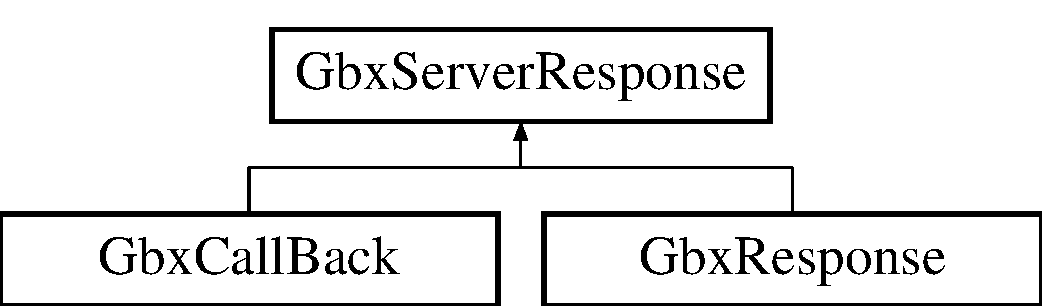
\includegraphics[height=2.000000cm]{classGbxServerResponse}
\end{center}
\end{figure}
\subsection*{Public Member Functions}
\begin{DoxyCompactItemize}
\item 
\hyperlink{classGbxServerResponse_a2198b6f6ca6b7da1ffd7bfa9a516d8b2}{Gbx\-Server\-Response} ()
\begin{DoxyCompactList}\small\item\em Empty constructor. \end{DoxyCompactList}\item 
\hyperlink{classGbxServerResponse_ad2a02192f5389a0fe10ea27cb24adedc}{$\sim$\-Gbx\-Server\-Response} ()
\item 
void \hyperlink{classGbxServerResponse_a1896da1a88aa07336829de953abe7364}{Set\-Raw} (char $\ast$response)
\begin{DoxyCompactList}\small\item\em Sets the raw message value. \end{DoxyCompactList}\item 
char $\ast$ \hyperlink{classGbxServerResponse_a3105f299a4f6a0d997f909415a467fd5}{Get\-Raw} ()
\begin{DoxyCompactList}\small\item\em Returns raw response (X\-M\-L). \end{DoxyCompactList}\item 
std\-::vector\\*
$<$ \hyperlink{classGbxResponseParameter}{Gbx\-Response\-Parameter} $>$ $\ast$ \hyperlink{classGbxServerResponse_ab791b8d9edb964b909d3c70753549668}{Get\-Parameters} ()
\begin{DoxyCompactList}\small\item\em Returns the extracted parameters. \end{DoxyCompactList}\end{DoxyCompactItemize}
\subsection*{Protected Member Functions}
\begin{DoxyCompactItemize}
\item 
\hyperlink{classGbxResponseParameter}{Gbx\-Response\-Parameter} \hyperlink{classGbxServerResponse_a22433a652ce9d4c7e9b834aa60c93c37}{extract\-Param} (pugi\-::xml\-\_\-node param)
\begin{DoxyCompactList}\small\item\em Extracts parameters from the raw data (X\-M\-L). \end{DoxyCompactList}\end{DoxyCompactItemize}
\subsection*{Protected Attributes}
\begin{DoxyCompactItemize}
\item 
char $\ast$ \hyperlink{classGbxServerResponse_aeee1fc539a5881334926e5c6789581bd}{data}
\begin{DoxyCompactList}\small\item\em Raw response data. \end{DoxyCompactList}\item 
std\-::vector\\*
$<$ \hyperlink{classGbxResponseParameter}{Gbx\-Response\-Parameter} $>$ $\ast$ \hyperlink{classGbxServerResponse_ad6fef5319c4da9461f4cd0d72d8b5ee8}{parameters} = new std\-::vector$<$\hyperlink{classGbxResponseParameter}{Gbx\-Response\-Parameter}$>$()
\begin{DoxyCompactList}\small\item\em List of parameters. \end{DoxyCompactList}\end{DoxyCompactItemize}


\subsection{Detailed Description}
Response from server, de-\/\-X\-M\-L-\/fies the response. 

\subsection{Constructor \& Destructor Documentation}
\hypertarget{classGbxServerResponse_a2198b6f6ca6b7da1ffd7bfa9a516d8b2}{\index{Gbx\-Server\-Response@{Gbx\-Server\-Response}!Gbx\-Server\-Response@{Gbx\-Server\-Response}}
\index{Gbx\-Server\-Response@{Gbx\-Server\-Response}!GbxServerResponse@{Gbx\-Server\-Response}}
\subsubsection[{Gbx\-Server\-Response}]{\setlength{\rightskip}{0pt plus 5cm}Gbx\-Server\-Response\-::\-Gbx\-Server\-Response (
\begin{DoxyParamCaption}
{}
\end{DoxyParamCaption}
)}}\label{classGbxServerResponse_a2198b6f6ca6b7da1ffd7bfa9a516d8b2}


Empty constructor. 

\hypertarget{classGbxServerResponse_ad2a02192f5389a0fe10ea27cb24adedc}{\index{Gbx\-Server\-Response@{Gbx\-Server\-Response}!$\sim$\-Gbx\-Server\-Response@{$\sim$\-Gbx\-Server\-Response}}
\index{$\sim$\-Gbx\-Server\-Response@{$\sim$\-Gbx\-Server\-Response}!GbxServerResponse@{Gbx\-Server\-Response}}
\subsubsection[{$\sim$\-Gbx\-Server\-Response}]{\setlength{\rightskip}{0pt plus 5cm}Gbx\-Server\-Response\-::$\sim$\-Gbx\-Server\-Response (
\begin{DoxyParamCaption}
{}
\end{DoxyParamCaption}
)}}\label{classGbxServerResponse_ad2a02192f5389a0fe10ea27cb24adedc}
Delets and nullifies the parameters. 

\subsection{Member Function Documentation}
\hypertarget{classGbxServerResponse_a22433a652ce9d4c7e9b834aa60c93c37}{\index{Gbx\-Server\-Response@{Gbx\-Server\-Response}!extract\-Param@{extract\-Param}}
\index{extract\-Param@{extract\-Param}!GbxServerResponse@{Gbx\-Server\-Response}}
\subsubsection[{extract\-Param}]{\setlength{\rightskip}{0pt plus 5cm}{\bf Gbx\-Response\-Parameter} Gbx\-Server\-Response\-::extract\-Param (
\begin{DoxyParamCaption}
\item[{pugi\-::xml\-\_\-node}]{param}
\end{DoxyParamCaption}
)\hspace{0.3cm}{\ttfamily [protected]}}}\label{classGbxServerResponse_a22433a652ce9d4c7e9b834aa60c93c37}


Extracts parameters from the raw data (X\-M\-L). 

\hypertarget{classGbxServerResponse_ab791b8d9edb964b909d3c70753549668}{\index{Gbx\-Server\-Response@{Gbx\-Server\-Response}!Get\-Parameters@{Get\-Parameters}}
\index{Get\-Parameters@{Get\-Parameters}!GbxServerResponse@{Gbx\-Server\-Response}}
\subsubsection[{Get\-Parameters}]{\setlength{\rightskip}{0pt plus 5cm}std\-::vector$<$ {\bf Gbx\-Response\-Parameter} $>$ $\ast$ Gbx\-Server\-Response\-::\-Get\-Parameters (
\begin{DoxyParamCaption}
{}
\end{DoxyParamCaption}
)}}\label{classGbxServerResponse_ab791b8d9edb964b909d3c70753549668}


Returns the extracted parameters. 

\hypertarget{classGbxServerResponse_a3105f299a4f6a0d997f909415a467fd5}{\index{Gbx\-Server\-Response@{Gbx\-Server\-Response}!Get\-Raw@{Get\-Raw}}
\index{Get\-Raw@{Get\-Raw}!GbxServerResponse@{Gbx\-Server\-Response}}
\subsubsection[{Get\-Raw}]{\setlength{\rightskip}{0pt plus 5cm}char $\ast$ Gbx\-Server\-Response\-::\-Get\-Raw (
\begin{DoxyParamCaption}
{}
\end{DoxyParamCaption}
)}}\label{classGbxServerResponse_a3105f299a4f6a0d997f909415a467fd5}


Returns raw response (X\-M\-L). 

\hypertarget{classGbxServerResponse_a1896da1a88aa07336829de953abe7364}{\index{Gbx\-Server\-Response@{Gbx\-Server\-Response}!Set\-Raw@{Set\-Raw}}
\index{Set\-Raw@{Set\-Raw}!GbxServerResponse@{Gbx\-Server\-Response}}
\subsubsection[{Set\-Raw}]{\setlength{\rightskip}{0pt plus 5cm}void Gbx\-Server\-Response\-::\-Set\-Raw (
\begin{DoxyParamCaption}
\item[{char $\ast$}]{response}
\end{DoxyParamCaption}
)}}\label{classGbxServerResponse_a1896da1a88aa07336829de953abe7364}


Sets the raw message value. 


\begin{DoxyParams}{Parameters}
{\em response} & Raw response from server (X\-M\-L). \\
\hline
\end{DoxyParams}


\subsection{Member Data Documentation}
\hypertarget{classGbxServerResponse_aeee1fc539a5881334926e5c6789581bd}{\index{Gbx\-Server\-Response@{Gbx\-Server\-Response}!data@{data}}
\index{data@{data}!GbxServerResponse@{Gbx\-Server\-Response}}
\subsubsection[{data}]{\setlength{\rightskip}{0pt plus 5cm}char$\ast$ Gbx\-Server\-Response\-::data\hspace{0.3cm}{\ttfamily [protected]}}}\label{classGbxServerResponse_aeee1fc539a5881334926e5c6789581bd}


Raw response data. 

\hypertarget{classGbxServerResponse_ad6fef5319c4da9461f4cd0d72d8b5ee8}{\index{Gbx\-Server\-Response@{Gbx\-Server\-Response}!parameters@{parameters}}
\index{parameters@{parameters}!GbxServerResponse@{Gbx\-Server\-Response}}
\subsubsection[{parameters}]{\setlength{\rightskip}{0pt plus 5cm}std\-::vector$<${\bf Gbx\-Response\-Parameter}$>$$\ast$ Gbx\-Server\-Response\-::parameters = new std\-::vector$<${\bf Gbx\-Response\-Parameter}$>$()\hspace{0.3cm}{\ttfamily [protected]}}}\label{classGbxServerResponse_ad6fef5319c4da9461f4cd0d72d8b5ee8}


List of parameters. 



The documentation for this class was generated from the following files\-:\begin{DoxyCompactItemize}
\item 
/home/travis/build/\-The\-Maximum/mania-\/pp/src/\-Gbx\-Remote/\-Server\-Response/\hyperlink{GbxServerResponse_8h}{Gbx\-Server\-Response.\-h}\item 
/home/travis/build/\-The\-Maximum/mania-\/pp/src/\-Gbx\-Remote/\-Server\-Response/\hyperlink{GbxServerResponse_8cpp}{Gbx\-Server\-Response.\-cpp}\end{DoxyCompactItemize}

\hypertarget{classGbxStructParameters}{\section{Gbx\-Struct\-Parameters Class Reference}
\label{classGbxStructParameters}\index{Gbx\-Struct\-Parameters@{Gbx\-Struct\-Parameters}}
}


List of struct parameters.  




{\ttfamily \#include $<$Gbx\-Parameters.\-h$>$}

\subsection*{Public Member Functions}
\begin{DoxyCompactItemize}
\item 
void \hyperlink{classGbxStructParameters_a1e045e8f50d30cdd810df10f3346bee4}{Put} (std\-::string text)
\begin{DoxyCompactList}\small\item\em Add parameter to the list. \end{DoxyCompactList}\item 
void \hyperlink{classGbxStructParameters_a97d487bfc030380abd4a6342139de30f}{Put} (std\-::string method\-Name, std\-::string parameter)
\begin{DoxyCompactList}\small\item\em Add parameter to the list. \end{DoxyCompactList}\item 
void \hyperlink{classGbxStructParameters_a6661fc06c7721857dd4e65a6edd8c8d5}{Put} (std\-::string method\-Name, \hyperlink{structParameter}{Parameter} parameter)
\begin{DoxyCompactList}\small\item\em Add parameter to the list. \end{DoxyCompactList}\item 
\hypertarget{classGbxStructParameters_a5d496ceb658abca1300ae093d26abedc}{std\-::vector$<$ std\-::string $>$ \hyperlink{classGbxStructParameters_a5d496ceb658abca1300ae093d26abedc}{Get\-Parameters} ()}\label{classGbxStructParameters_a5d496ceb658abca1300ae093d26abedc}

\begin{DoxyCompactList}\small\item\em Return the current list of parameters. \end{DoxyCompactList}\end{DoxyCompactItemize}
\subsection*{Private Attributes}
\begin{DoxyCompactItemize}
\item 
\hypertarget{classGbxStructParameters_a28bc30c4732e983831d05ac4591a3aec}{std\-::vector$<$ std\-::string $>$ \hyperlink{classGbxStructParameters_a28bc30c4732e983831d05ac4591a3aec}{parameters} = std\-::vector$<$std\-::string$>$()}\label{classGbxStructParameters_a28bc30c4732e983831d05ac4591a3aec}

\begin{DoxyCompactList}\small\item\em List of parameters. \end{DoxyCompactList}\end{DoxyCompactItemize}


\subsection{Detailed Description}
List of struct parameters. 

\subsection{Member Function Documentation}
\hypertarget{classGbxStructParameters_a1e045e8f50d30cdd810df10f3346bee4}{\index{Gbx\-Struct\-Parameters@{Gbx\-Struct\-Parameters}!Put@{Put}}
\index{Put@{Put}!GbxStructParameters@{Gbx\-Struct\-Parameters}}
\subsubsection[{Put}]{\setlength{\rightskip}{0pt plus 5cm}void Gbx\-Struct\-Parameters\-::\-Put (
\begin{DoxyParamCaption}
\item[{std\-::string}]{text}
\end{DoxyParamCaption}
)\hspace{0.3cm}{\ttfamily [inline]}}}\label{classGbxStructParameters_a1e045e8f50d30cdd810df10f3346bee4}


Add parameter to the list. 


\begin{DoxyParams}{Parameters}
{\em text} & \hyperlink{structParameter}{Parameter} X\-M\-L. \\
\hline
\end{DoxyParams}
\hypertarget{classGbxStructParameters_a97d487bfc030380abd4a6342139de30f}{\index{Gbx\-Struct\-Parameters@{Gbx\-Struct\-Parameters}!Put@{Put}}
\index{Put@{Put}!GbxStructParameters@{Gbx\-Struct\-Parameters}}
\subsubsection[{Put}]{\setlength{\rightskip}{0pt plus 5cm}void Gbx\-Struct\-Parameters\-::\-Put (
\begin{DoxyParamCaption}
\item[{std\-::string}]{method\-Name, }
\item[{std\-::string}]{parameter}
\end{DoxyParamCaption}
)\hspace{0.3cm}{\ttfamily [inline]}}}\label{classGbxStructParameters_a97d487bfc030380abd4a6342139de30f}


Add parameter to the list. 


\begin{DoxyParams}{Parameters}
{\em method\-Name} & Method name. \\
\hline
{\em parameter} & \hyperlink{structParameter}{Parameter}. \\
\hline
\end{DoxyParams}
\hypertarget{classGbxStructParameters_a6661fc06c7721857dd4e65a6edd8c8d5}{\index{Gbx\-Struct\-Parameters@{Gbx\-Struct\-Parameters}!Put@{Put}}
\index{Put@{Put}!GbxStructParameters@{Gbx\-Struct\-Parameters}}
\subsubsection[{Put}]{\setlength{\rightskip}{0pt plus 5cm}void Gbx\-Struct\-Parameters\-::\-Put (
\begin{DoxyParamCaption}
\item[{std\-::string}]{method\-Name, }
\item[{{\bf Parameter}}]{parameter}
\end{DoxyParamCaption}
)}}\label{classGbxStructParameters_a6661fc06c7721857dd4e65a6edd8c8d5}


Add parameter to the list. 


\begin{DoxyParams}{Parameters}
{\em method\-Name} & Method name. \\
\hline
{\em parameter} & \hyperlink{structParameter}{Parameter}. \\
\hline
\end{DoxyParams}


The documentation for this class was generated from the following files\-:\begin{DoxyCompactItemize}
\item 
/home/travis/build/\-The\-Maximum/mania-\/pp/src/\-Gbx\-Remote/\-Parameters/Gbx\-Parameters.\-h\item 
/home/travis/build/\-The\-Maximum/mania-\/pp/src/\-Gbx\-Remote/\-Parameters/Gbx\-Parameters.\-cpp\end{DoxyCompactItemize}

\hypertarget{structGitVersion}{\section{Git\-Version Struct Reference}
\label{structGitVersion}\index{Git\-Version@{Git\-Version}}
}


Contains information about a Git release (version).  




{\ttfamily \#include $<$Version\-Checker.\-h$>$}

\subsection*{Public Attributes}
\begin{DoxyCompactItemize}
\item 
\hypertarget{structGitVersion_ad47dce1972d1058648429996c6ed02b0}{std\-::string \hyperlink{structGitVersion_ad47dce1972d1058648429996c6ed02b0}{Repository}}\label{structGitVersion_ad47dce1972d1058648429996c6ed02b0}

\begin{DoxyCompactList}\small\item\em Name of the Git\-Hub repository. \end{DoxyCompactList}\item 
\hypertarget{structGitVersion_ad436b796df94381fe3af70559868ed55}{std\-::string \hyperlink{structGitVersion_ad436b796df94381fe3af70559868ed55}{Tag}}\label{structGitVersion_ad436b796df94381fe3af70559868ed55}

\begin{DoxyCompactList}\small\item\em Tag version. \end{DoxyCompactList}\item 
\hypertarget{structGitVersion_a437b0aaee8685d61cccde69ad4ae73ec}{std\-::string \hyperlink{structGitVersion_a437b0aaee8685d61cccde69ad4ae73ec}{Name}}\label{structGitVersion_a437b0aaee8685d61cccde69ad4ae73ec}

\begin{DoxyCompactList}\small\item\em Tag name (description). \end{DoxyCompactList}\item 
\hypertarget{structGitVersion_a0a7fcfae969cad2cb90dc0353df5bf49}{std\-::string \hyperlink{structGitVersion_a0a7fcfae969cad2cb90dc0353df5bf49}{Commit}}\label{structGitVersion_a0a7fcfae969cad2cb90dc0353df5bf49}

\begin{DoxyCompactList}\small\item\em S\-H\-A commit. \end{DoxyCompactList}\item 
\hypertarget{structGitVersion_a632eaf068f15348c372389d86b310525}{bool \hyperlink{structGitVersion_a632eaf068f15348c372389d86b310525}{Pre\-Release}}\label{structGitVersion_a632eaf068f15348c372389d86b310525}

\begin{DoxyCompactList}\small\item\em Is pre-\/release?. \end{DoxyCompactList}\end{DoxyCompactItemize}


\subsection{Detailed Description}
Contains information about a Git release (version). 

The documentation for this struct was generated from the following file\-:\begin{DoxyCompactItemize}
\item 
/home/travis/build/\-The\-Maximum/mania-\/pp/src/\-Version/Version\-Checker.\-h\end{DoxyCompactItemize}

\hypertarget{classHex}{\section{Hex Class Reference}
\label{classHex}\index{Hex@{Hex}}
}


Utility to print char arrays/pointers as hexadecimal values.  




{\ttfamily \#include $<$Hex.\-h$>$}

\subsection*{Static Public Member Functions}
\begin{DoxyCompactItemize}
\item 
static void \hyperlink{classHex_a875b48852fbd0032d85d01286d8653c1}{Print} (char message\mbox{[}$\,$\mbox{]}, int message\-Length)
\begin{DoxyCompactList}\small\item\em Prints char array as hexadecimal values. \end{DoxyCompactList}\item 
static void \hyperlink{classHex_a7a955b79027e7bb270b96d0f13e26043}{Print} (char $\ast$data)
\begin{DoxyCompactList}\small\item\em Prints char pointer as hexadecimal values. \end{DoxyCompactList}\end{DoxyCompactItemize}


\subsection{Detailed Description}
Utility to print char arrays/pointers as hexadecimal values. 

\subsection{Member Function Documentation}
\hypertarget{classHex_a875b48852fbd0032d85d01286d8653c1}{\index{Hex@{Hex}!Print@{Print}}
\index{Print@{Print}!Hex@{Hex}}
\subsubsection[{Print}]{\setlength{\rightskip}{0pt plus 5cm}static void Hex\-::\-Print (
\begin{DoxyParamCaption}
\item[{char}]{message\mbox{[}$\,$\mbox{]}, }
\item[{int}]{message\-Length}
\end{DoxyParamCaption}
)\hspace{0.3cm}{\ttfamily [inline]}, {\ttfamily [static]}}}\label{classHex_a875b48852fbd0032d85d01286d8653c1}


Prints char array as hexadecimal values. 

For printing the char array as hexadecimal, it uses the std\-::hex option. The char array is casted and printed char by char.


\begin{DoxyParams}{Parameters}
{\em message} & Char array with message to be displayed. \\
\hline
{\em message\-Length} & Length of the char array. \\
\hline
\end{DoxyParams}
\hypertarget{classHex_a7a955b79027e7bb270b96d0f13e26043}{\index{Hex@{Hex}!Print@{Print}}
\index{Print@{Print}!Hex@{Hex}}
\subsubsection[{Print}]{\setlength{\rightskip}{0pt plus 5cm}static void Hex\-::\-Print (
\begin{DoxyParamCaption}
\item[{char $\ast$}]{data}
\end{DoxyParamCaption}
)\hspace{0.3cm}{\ttfamily [inline]}, {\ttfamily [static]}}}\label{classHex_a7a955b79027e7bb270b96d0f13e26043}


Prints char pointer as hexadecimal values. 

Casts the pointer to a char array and uses the char array version of the function.


\begin{DoxyParams}{Parameters}
{\em data} & Char pointer with message to be displayed. \\
\hline
\end{DoxyParams}


The documentation for this class was generated from the following file\-:\begin{DoxyCompactItemize}
\item 
/home/travis/build/\-The\-Maximum/mania-\/pp/src/\-Utils/\hyperlink{Hex_8h}{Hex.\-h}\end{DoxyCompactItemize}

\hypertarget{classLogging}{\section{Logging Class Reference}
\label{classLogging}\index{Logging@{Logging}}
}


Utility to print information to the console.  




{\ttfamily \#include $<$Logging.\-h$>$}

\subsection*{Static Public Member Functions}
\begin{DoxyCompactItemize}
\item 
static void \hyperlink{classLogging_a171703bedcbf215f0e6334f29c8281b5}{Print\-Error} (\hyperlink{structGbxError}{Gbx\-Error} $\ast$error)
\begin{DoxyCompactList}\small\item\em Prints error to console. \end{DoxyCompactList}\item 
static void \hyperlink{classLogging_ac1397db1b8ea6625f7dd2616f530cd7d}{Print\-Error} (int number, std\-::string message)
\begin{DoxyCompactList}\small\item\em Prints error to console. \end{DoxyCompactList}\item 
\hypertarget{classLogging_a889f2ad8f991afdf0959cb1cad736fa7}{static void \hyperlink{classLogging_a889f2ad8f991afdf0959cb1cad736fa7}{Print\-O\-K\-Flush} ()}\label{classLogging_a889f2ad8f991afdf0959cb1cad736fa7}

\begin{DoxyCompactList}\small\item\em Prints O\-K. in \mbox{[} \mbox{]}-\/spaces in console. \end{DoxyCompactList}\item 
\hypertarget{classLogging_add0483bd14aef74ec988606cd7dbfc4b}{static void \hyperlink{classLogging_add0483bd14aef74ec988606cd7dbfc4b}{Print\-Failed\-Flush} ()}\label{classLogging_add0483bd14aef74ec988606cd7dbfc4b}

\begin{DoxyCompactList}\small\item\em Prints Failed! in \mbox{[} \mbox{]}-\/spaces in console. \end{DoxyCompactList}\item 
static void \hyperlink{classLogging_a1f8609052e40055fb9ef3ddd40d0620e}{Print\-Parameter} (\hyperlink{classGbxResponseParameter}{Gbx\-Response\-Parameter} parameter, int param\-Id, std\-::string spaces=\char`\"{}    \char`\"{}, std\-::string parameter\-Name=\char`\"{}\char`\"{})
\begin{DoxyCompactList}\small\item\em Prints a \hyperlink{classGbxResponseParameter}{Gbx\-Response\-Parameter} (for D\-E\-B\-U\-G purposes). \end{DoxyCompactList}\end{DoxyCompactItemize}


\subsection{Detailed Description}
Utility to print information to the console. 

\subsection{Member Function Documentation}
\hypertarget{classLogging_a171703bedcbf215f0e6334f29c8281b5}{\index{Logging@{Logging}!Print\-Error@{Print\-Error}}
\index{Print\-Error@{Print\-Error}!Logging@{Logging}}
\subsubsection[{Print\-Error}]{\setlength{\rightskip}{0pt plus 5cm}static void Logging\-::\-Print\-Error (
\begin{DoxyParamCaption}
\item[{{\bf Gbx\-Error} $\ast$}]{error}
\end{DoxyParamCaption}
)\hspace{0.3cm}{\ttfamily [inline]}, {\ttfamily [static]}}}\label{classLogging_a171703bedcbf215f0e6334f29c8281b5}


Prints error to console. 


\begin{DoxyParams}{Parameters}
{\em error} & Error structure. \\
\hline
\end{DoxyParams}
\hypertarget{classLogging_ac1397db1b8ea6625f7dd2616f530cd7d}{\index{Logging@{Logging}!Print\-Error@{Print\-Error}}
\index{Print\-Error@{Print\-Error}!Logging@{Logging}}
\subsubsection[{Print\-Error}]{\setlength{\rightskip}{0pt plus 5cm}static void Logging\-::\-Print\-Error (
\begin{DoxyParamCaption}
\item[{int}]{number, }
\item[{std\-::string}]{message}
\end{DoxyParamCaption}
)\hspace{0.3cm}{\ttfamily [inline]}, {\ttfamily [static]}}}\label{classLogging_ac1397db1b8ea6625f7dd2616f530cd7d}


Prints error to console. 


\begin{DoxyParams}{Parameters}
{\em number} & Error number. \\
\hline
{\em message} & Error message. \\
\hline
\end{DoxyParams}
\hypertarget{classLogging_a1f8609052e40055fb9ef3ddd40d0620e}{\index{Logging@{Logging}!Print\-Parameter@{Print\-Parameter}}
\index{Print\-Parameter@{Print\-Parameter}!Logging@{Logging}}
\subsubsection[{Print\-Parameter}]{\setlength{\rightskip}{0pt plus 5cm}static void Logging\-::\-Print\-Parameter (
\begin{DoxyParamCaption}
\item[{{\bf Gbx\-Response\-Parameter}}]{parameter, }
\item[{int}]{param\-Id, }
\item[{std\-::string}]{spaces = {\ttfamily \char`\"{}~~~~\char`\"{}}, }
\item[{std\-::string}]{parameter\-Name = {\ttfamily \char`\"{}\char`\"{}}}
\end{DoxyParamCaption}
)\hspace{0.3cm}{\ttfamily [inline]}, {\ttfamily [static]}}}\label{classLogging_a1f8609052e40055fb9ef3ddd40d0620e}


Prints a \hyperlink{classGbxResponseParameter}{Gbx\-Response\-Parameter} (for D\-E\-B\-U\-G purposes). 


\begin{DoxyParams}{Parameters}
{\em parameter} & Parameter to be printed. \\
\hline
{\em param\-Id} & Number of the parameter. \\
\hline
{\em spaces} & Spaces to be put before the parameter information. \\
\hline
{\em parameter\-Name} & Name of the parameter (struct value only). \\
\hline
\end{DoxyParams}


The documentation for this class was generated from the following file\-:\begin{DoxyCompactItemize}
\item 
/home/travis/build/\-The\-Maximum/mania-\/pp/src/\-Utils/Logging.\-h\end{DoxyCompactItemize}

\hypertarget{structManiaLinkPageAnswer}{\section{Mania\-Link\-Page\-Answer Struct Reference}
\label{structManiaLinkPageAnswer}\index{Mania\-Link\-Page\-Answer@{Mania\-Link\-Page\-Answer}}
}


Struct with a Mania\-Link page answer.  




{\ttfamily \#include $<$Structs.\-h$>$}

\subsection*{Public Attributes}
\begin{DoxyCompactItemize}
\item 
\hypertarget{structManiaLinkPageAnswer_afb091a6cd4c5879232564816ce18422d}{\hyperlink{structPlayer}{Player} \hyperlink{structManiaLinkPageAnswer_afb091a6cd4c5879232564816ce18422d}{Answering\-Player}}\label{structManiaLinkPageAnswer_afb091a6cd4c5879232564816ce18422d}

\begin{DoxyCompactList}\small\item\em \hyperlink{structPlayer}{Player} answering. \end{DoxyCompactList}\item 
\hypertarget{structManiaLinkPageAnswer_a270ed5e3cf6a5dd74cca2c6c1d007ae1}{int \hyperlink{structManiaLinkPageAnswer_a270ed5e3cf6a5dd74cca2c6c1d007ae1}{Result}}\label{structManiaLinkPageAnswer_a270ed5e3cf6a5dd74cca2c6c1d007ae1}

\begin{DoxyCompactList}\small\item\em Answering result. \end{DoxyCompactList}\end{DoxyCompactItemize}


\subsection{Detailed Description}
Struct with a Mania\-Link page answer. 

The documentation for this struct was generated from the following file\-:\begin{DoxyCompactItemize}
\item 
/home/travis/build/\-The\-Maximum/mania-\/pp/src/\-Methods/Structs.\-h\end{DoxyCompactItemize}

\hypertarget{classManiaPP}{\section{Mania\-P\-P Class Reference}
\label{classManiaPP}\index{Mania\-P\-P@{Mania\-P\-P}}
}


Main class.  




{\ttfamily \#include $<$Mania\-P\-P.\-h$>$}

\subsection*{Public Member Functions}
\begin{DoxyCompactItemize}
\item 
\hyperlink{classManiaPP_ae56f6623dc89f2c0b75bec631cfc2d19}{Mania\-P\-P} ()
\begin{DoxyCompactList}\small\item\em Sets up the several variables needed to run the software. \end{DoxyCompactList}\item 
\hyperlink{classManiaPP_a1c78c3b51db550609011fb6fdcb26ec8}{$\sim$\-Mania\-P\-P} ()
\begin{DoxyCompactList}\small\item\em Destructs the pointers in the main class. \end{DoxyCompactList}\item 
bool \hyperlink{classManiaPP_a22561171876e54dbf633c70d9924c06a}{Connect\-To\-Server} ()
\begin{DoxyCompactList}\small\item\em Connects and authenticates with the server. \end{DoxyCompactList}\item 
void \hyperlink{classManiaPP_a56d2774a29f21b3a164ae1f7ea6bd88b}{Print\-Server\-Info} ()
\begin{DoxyCompactList}\small\item\em Prints information about the server. \end{DoxyCompactList}\item 
void \hyperlink{classManiaPP_a8dff9e8e3835c3cac0df105a7bcce43c}{Main\-Loop} ()
\begin{DoxyCompactList}\small\item\em Performing our tasks ... \end{DoxyCompactList}\item 
void \hyperlink{classManiaPP_a87fd53fffe4a1840834a90ab575f5ce6}{Terminate} ()
\begin{DoxyCompactList}\small\item\em Disconnects the software from the server. \end{DoxyCompactList}\item 
void \hyperlink{classManiaPP_a3548cbafbf949dbb9d210c08adb5f7de}{Print\-Parameter} (\hyperlink{classGbxResponseParameter}{Gbx\-Response\-Parameter} parameter, int param\-Id, std\-::string spaces=\char`\"{}    \char`\"{})
\end{DoxyCompactItemize}
\subsection*{Private Member Functions}
\begin{DoxyCompactItemize}
\item 
void \hyperlink{classManiaPP_aede94c0b982250de19186d447542e479}{retrieve\-Player\-List} ()
\begin{DoxyCompactList}\small\item\em Gets a list of current players from the server. \end{DoxyCompactList}\item 
void \hyperlink{classManiaPP_a18582fa28b259c22a8a8d526af62123a}{retrieve\-Map\-List} ()
\begin{DoxyCompactList}\small\item\em Gets a list of current maps from the server. \end{DoxyCompactList}\end{DoxyCompactItemize}
\subsection*{Private Attributes}
\begin{DoxyCompactItemize}
\item 
\hyperlink{classConfig}{Config} $\ast$ \hyperlink{classManiaPP_a9a91437fa70afd52c2dce19298888e36}{config}
\begin{DoxyCompactList}\small\item\em Contains the configuration for the software. \end{DoxyCompactList}\item 
\hyperlink{classLogging}{Logging} $\ast$ \hyperlink{classManiaPP_aa4cea090301bdf0bf652ad377e7b01c0}{logging}
\begin{DoxyCompactList}\small\item\em Contains functions to log information. \end{DoxyCompactList}\item 
\hyperlink{classGbxRemote}{Gbx\-Remote} $\ast$ \hyperlink{classManiaPP_ab81311d6901990cb99a7a30e0cbaab11}{server}
\begin{DoxyCompactList}\small\item\em Contains the connection with the server and its methods. \end{DoxyCompactList}\item 
std\-::map$<$ std\-::string, \hyperlink{structPlayer}{Player} $>$ $\ast$ \hyperlink{classManiaPP_a45712ccfa91b20242b39cb1164d305d8}{players}
\begin{DoxyCompactList}\small\item\em Contains the list of players currently on the server. \end{DoxyCompactList}\item 
std\-::map$<$ std\-::string, \hyperlink{structMap}{Map} $>$ $\ast$ \hyperlink{classManiaPP_a903ccf13c65b15c99595cb571214799d}{maps}
\begin{DoxyCompactList}\small\item\em Contains the list of players currently on the server. \end{DoxyCompactList}\end{DoxyCompactItemize}


\subsection{Detailed Description}
Main class. 

\subsection{Constructor \& Destructor Documentation}
\hypertarget{classManiaPP_ae56f6623dc89f2c0b75bec631cfc2d19}{\index{Mania\-P\-P@{Mania\-P\-P}!Mania\-P\-P@{Mania\-P\-P}}
\index{Mania\-P\-P@{Mania\-P\-P}!ManiaPP@{Mania\-P\-P}}
\subsubsection[{Mania\-P\-P}]{\setlength{\rightskip}{0pt plus 5cm}Mania\-P\-P\-::\-Mania\-P\-P (
\begin{DoxyParamCaption}
{}
\end{DoxyParamCaption}
)}}\label{classManiaPP_ae56f6623dc89f2c0b75bec631cfc2d19}


Sets up the several variables needed to run the software. 

\hypertarget{classManiaPP_a1c78c3b51db550609011fb6fdcb26ec8}{\index{Mania\-P\-P@{Mania\-P\-P}!$\sim$\-Mania\-P\-P@{$\sim$\-Mania\-P\-P}}
\index{$\sim$\-Mania\-P\-P@{$\sim$\-Mania\-P\-P}!ManiaPP@{Mania\-P\-P}}
\subsubsection[{$\sim$\-Mania\-P\-P}]{\setlength{\rightskip}{0pt plus 5cm}Mania\-P\-P\-::$\sim$\-Mania\-P\-P (
\begin{DoxyParamCaption}
{}
\end{DoxyParamCaption}
)}}\label{classManiaPP_a1c78c3b51db550609011fb6fdcb26ec8}


Destructs the pointers in the main class. 



\subsection{Member Function Documentation}
\hypertarget{classManiaPP_a22561171876e54dbf633c70d9924c06a}{\index{Mania\-P\-P@{Mania\-P\-P}!Connect\-To\-Server@{Connect\-To\-Server}}
\index{Connect\-To\-Server@{Connect\-To\-Server}!ManiaPP@{Mania\-P\-P}}
\subsubsection[{Connect\-To\-Server}]{\setlength{\rightskip}{0pt plus 5cm}bool Mania\-P\-P\-::\-Connect\-To\-Server (
\begin{DoxyParamCaption}
{}
\end{DoxyParamCaption}
)}}\label{classManiaPP_a22561171876e54dbf633c70d9924c06a}


Connects and authenticates with the server. 

\hypertarget{classManiaPP_a8dff9e8e3835c3cac0df105a7bcce43c}{\index{Mania\-P\-P@{Mania\-P\-P}!Main\-Loop@{Main\-Loop}}
\index{Main\-Loop@{Main\-Loop}!ManiaPP@{Mania\-P\-P}}
\subsubsection[{Main\-Loop}]{\setlength{\rightskip}{0pt plus 5cm}void Mania\-P\-P\-::\-Main\-Loop (
\begin{DoxyParamCaption}
{}
\end{DoxyParamCaption}
)}}\label{classManiaPP_a8dff9e8e3835c3cac0df105a7bcce43c}


Performing our tasks ... 

\hypertarget{classManiaPP_a3548cbafbf949dbb9d210c08adb5f7de}{\index{Mania\-P\-P@{Mania\-P\-P}!Print\-Parameter@{Print\-Parameter}}
\index{Print\-Parameter@{Print\-Parameter}!ManiaPP@{Mania\-P\-P}}
\subsubsection[{Print\-Parameter}]{\setlength{\rightskip}{0pt plus 5cm}void Mania\-P\-P\-::\-Print\-Parameter (
\begin{DoxyParamCaption}
\item[{{\bf Gbx\-Response\-Parameter}}]{parameter, }
\item[{int}]{param\-Id, }
\item[{std\-::string}]{spaces = {\ttfamily \char`\"{}~~~~\char`\"{}}}
\end{DoxyParamCaption}
)}}\label{classManiaPP_a3548cbafbf949dbb9d210c08adb5f7de}
\hypertarget{classManiaPP_a56d2774a29f21b3a164ae1f7ea6bd88b}{\index{Mania\-P\-P@{Mania\-P\-P}!Print\-Server\-Info@{Print\-Server\-Info}}
\index{Print\-Server\-Info@{Print\-Server\-Info}!ManiaPP@{Mania\-P\-P}}
\subsubsection[{Print\-Server\-Info}]{\setlength{\rightskip}{0pt plus 5cm}void Mania\-P\-P\-::\-Print\-Server\-Info (
\begin{DoxyParamCaption}
{}
\end{DoxyParamCaption}
)}}\label{classManiaPP_a56d2774a29f21b3a164ae1f7ea6bd88b}


Prints information about the server. 

\hypertarget{classManiaPP_a18582fa28b259c22a8a8d526af62123a}{\index{Mania\-P\-P@{Mania\-P\-P}!retrieve\-Map\-List@{retrieve\-Map\-List}}
\index{retrieve\-Map\-List@{retrieve\-Map\-List}!ManiaPP@{Mania\-P\-P}}
\subsubsection[{retrieve\-Map\-List}]{\setlength{\rightskip}{0pt plus 5cm}void Mania\-P\-P\-::retrieve\-Map\-List (
\begin{DoxyParamCaption}
{}
\end{DoxyParamCaption}
)\hspace{0.3cm}{\ttfamily [private]}}}\label{classManiaPP_a18582fa28b259c22a8a8d526af62123a}


Gets a list of current maps from the server. 

\hypertarget{classManiaPP_aede94c0b982250de19186d447542e479}{\index{Mania\-P\-P@{Mania\-P\-P}!retrieve\-Player\-List@{retrieve\-Player\-List}}
\index{retrieve\-Player\-List@{retrieve\-Player\-List}!ManiaPP@{Mania\-P\-P}}
\subsubsection[{retrieve\-Player\-List}]{\setlength{\rightskip}{0pt plus 5cm}void Mania\-P\-P\-::retrieve\-Player\-List (
\begin{DoxyParamCaption}
{}
\end{DoxyParamCaption}
)\hspace{0.3cm}{\ttfamily [private]}}}\label{classManiaPP_aede94c0b982250de19186d447542e479}


Gets a list of current players from the server. 

\hypertarget{classManiaPP_a87fd53fffe4a1840834a90ab575f5ce6}{\index{Mania\-P\-P@{Mania\-P\-P}!Terminate@{Terminate}}
\index{Terminate@{Terminate}!ManiaPP@{Mania\-P\-P}}
\subsubsection[{Terminate}]{\setlength{\rightskip}{0pt plus 5cm}void Mania\-P\-P\-::\-Terminate (
\begin{DoxyParamCaption}
{}
\end{DoxyParamCaption}
)}}\label{classManiaPP_a87fd53fffe4a1840834a90ab575f5ce6}


Disconnects the software from the server. 



\subsection{Member Data Documentation}
\hypertarget{classManiaPP_a9a91437fa70afd52c2dce19298888e36}{\index{Mania\-P\-P@{Mania\-P\-P}!config@{config}}
\index{config@{config}!ManiaPP@{Mania\-P\-P}}
\subsubsection[{config}]{\setlength{\rightskip}{0pt plus 5cm}{\bf Config}$\ast$ Mania\-P\-P\-::config\hspace{0.3cm}{\ttfamily [private]}}}\label{classManiaPP_a9a91437fa70afd52c2dce19298888e36}


Contains the configuration for the software. 

\hypertarget{classManiaPP_aa4cea090301bdf0bf652ad377e7b01c0}{\index{Mania\-P\-P@{Mania\-P\-P}!logging@{logging}}
\index{logging@{logging}!ManiaPP@{Mania\-P\-P}}
\subsubsection[{logging}]{\setlength{\rightskip}{0pt plus 5cm}{\bf Logging}$\ast$ Mania\-P\-P\-::logging\hspace{0.3cm}{\ttfamily [private]}}}\label{classManiaPP_aa4cea090301bdf0bf652ad377e7b01c0}


Contains functions to log information. 

\hypertarget{classManiaPP_a903ccf13c65b15c99595cb571214799d}{\index{Mania\-P\-P@{Mania\-P\-P}!maps@{maps}}
\index{maps@{maps}!ManiaPP@{Mania\-P\-P}}
\subsubsection[{maps}]{\setlength{\rightskip}{0pt plus 5cm}std\-::map$<$std\-::string, {\bf Map}$>$$\ast$ Mania\-P\-P\-::maps\hspace{0.3cm}{\ttfamily [private]}}}\label{classManiaPP_a903ccf13c65b15c99595cb571214799d}


Contains the list of players currently on the server. 

\hypertarget{classManiaPP_a45712ccfa91b20242b39cb1164d305d8}{\index{Mania\-P\-P@{Mania\-P\-P}!players@{players}}
\index{players@{players}!ManiaPP@{Mania\-P\-P}}
\subsubsection[{players}]{\setlength{\rightskip}{0pt plus 5cm}std\-::map$<$std\-::string, {\bf Player}$>$$\ast$ Mania\-P\-P\-::players\hspace{0.3cm}{\ttfamily [private]}}}\label{classManiaPP_a45712ccfa91b20242b39cb1164d305d8}


Contains the list of players currently on the server. 

\hypertarget{classManiaPP_ab81311d6901990cb99a7a30e0cbaab11}{\index{Mania\-P\-P@{Mania\-P\-P}!server@{server}}
\index{server@{server}!ManiaPP@{Mania\-P\-P}}
\subsubsection[{server}]{\setlength{\rightskip}{0pt plus 5cm}{\bf Gbx\-Remote}$\ast$ Mania\-P\-P\-::server\hspace{0.3cm}{\ttfamily [private]}}}\label{classManiaPP_ab81311d6901990cb99a7a30e0cbaab11}


Contains the connection with the server and its methods. 



The documentation for this class was generated from the following files\-:\begin{DoxyCompactItemize}
\item 
/home/travis/build/\-The\-Maximum/mania-\/pp/src/\hyperlink{ManiaPP_8h}{Mania\-P\-P.\-h}\item 
/home/travis/build/\-The\-Maximum/mania-\/pp/src/\hyperlink{ManiaPP_8cpp}{Mania\-P\-P.\-cpp}\end{DoxyCompactItemize}

\hypertarget{structMap}{\section{Map Struct Reference}
\label{structMap}\index{Map@{Map}}
}


Contains all information about a map in easy-\/to-\/use format.  




{\ttfamily \#include $<$Map.\-h$>$}

\subsection*{Public Member Functions}
\begin{DoxyCompactItemize}
\item 
\hypertarget{structMap_a0f5ad0fd4563497b4214038cbca8b582}{\hyperlink{structMap_a0f5ad0fd4563497b4214038cbca8b582}{Map} ()}\label{structMap_a0f5ad0fd4563497b4214038cbca8b582}

\begin{DoxyCompactList}\small\item\em Constructs a \hyperlink{structMap}{Map} object without input. \end{DoxyCompactList}\item 
\hyperlink{structMap_a95a2cda9b2746b5ba75e811930559c1f}{Map} (std\-::map$<$ std\-::string, \hyperlink{classGbxResponseParameter}{Gbx\-Response\-Parameter} $>$ server\-Struct)
\begin{DoxyCompactList}\small\item\em Formats a server response into a usable form. \end{DoxyCompactList}\item 
void \hyperlink{structMap_ac8e78e5d9ba3951db798736fc33e907e}{Map\-Detailed} (std\-::map$<$ std\-::string, \hyperlink{classGbxResponseParameter}{Gbx\-Response\-Parameter} $>$ server\-Struct)
\begin{DoxyCompactList}\small\item\em Formats a server response into a usable form. \end{DoxyCompactList}\item 
void \hyperlink{structMap_af83b3a784e6fa9404c1940a2ca1b68a8}{Set\-Id} (int id)
\begin{DoxyCompactList}\small\item\em Set database identifier value. \end{DoxyCompactList}\end{DoxyCompactItemize}
\subsection*{Public Attributes}
\begin{DoxyCompactItemize}
\item 
\hypertarget{structMap_af718266059246076a208fa4323e187f4}{int \hyperlink{structMap_af718266059246076a208fa4323e187f4}{Id} = 0}\label{structMap_af718266059246076a208fa4323e187f4}

\begin{DoxyCompactList}\small\item\em \hyperlink{structMap}{Map} identifier (on database). \end{DoxyCompactList}\item 
\hypertarget{structMap_aeeaed7abcf77e119d5f59c0918183834}{std\-::string \hyperlink{structMap_aeeaed7abcf77e119d5f59c0918183834}{U\-Id}}\label{structMap_aeeaed7abcf77e119d5f59c0918183834}

\begin{DoxyCompactList}\small\item\em Unique map identifier. \end{DoxyCompactList}\item 
\hypertarget{structMap_ab1a5bf049a4b74e704128d31e9b53b8c}{std\-::string \hyperlink{structMap_ab1a5bf049a4b74e704128d31e9b53b8c}{Name}}\label{structMap_ab1a5bf049a4b74e704128d31e9b53b8c}

\begin{DoxyCompactList}\small\item\em \hyperlink{structMap}{Map} name. \end{DoxyCompactList}\item 
\hypertarget{structMap_a0ec301bf4f1d129cd9bc50999581eec9}{std\-::string \hyperlink{structMap_a0ec301bf4f1d129cd9bc50999581eec9}{File\-Name}}\label{structMap_a0ec301bf4f1d129cd9bc50999581eec9}

\begin{DoxyCompactList}\small\item\em File name. \end{DoxyCompactList}\item 
\hypertarget{structMap_acbaadf8f635b04a1229fa01f6ec4c4dc}{std\-::string \hyperlink{structMap_acbaadf8f635b04a1229fa01f6ec4c4dc}{Environment}}\label{structMap_acbaadf8f635b04a1229fa01f6ec4c4dc}

\begin{DoxyCompactList}\small\item\em Game environment. \end{DoxyCompactList}\item 
\hypertarget{structMap_a1eb246326a4ec70df2dc71887efca5c9}{std\-::string \hyperlink{structMap_a1eb246326a4ec70df2dc71887efca5c9}{Author}}\label{structMap_a1eb246326a4ec70df2dc71887efca5c9}

\begin{DoxyCompactList}\small\item\em Login of the author. \end{DoxyCompactList}\item 
\hypertarget{structMap_a769a574be92aa024f7804627c167ceff}{int \hyperlink{structMap_a769a574be92aa024f7804627c167ceff}{Gold\-Time}}\label{structMap_a769a574be92aa024f7804627c167ceff}

\begin{DoxyCompactList}\small\item\em \hyperlink{classTime}{Time} of the gold medal. \end{DoxyCompactList}\item 
\hypertarget{structMap_aa9a7d229fb6b41092fb527bbcc913faf}{int \hyperlink{structMap_aa9a7d229fb6b41092fb527bbcc913faf}{Copper\-Price}}\label{structMap_aa9a7d229fb6b41092fb527bbcc913faf}

\begin{DoxyCompactList}\small\item\em Copper price. \end{DoxyCompactList}\item 
\hypertarget{structMap_a23d051ee3c7cfa606082e700099563b0}{std\-::string \hyperlink{structMap_a23d051ee3c7cfa606082e700099563b0}{Map\-Type}}\label{structMap_a23d051ee3c7cfa606082e700099563b0}

\begin{DoxyCompactList}\small\item\em Type of the map. \end{DoxyCompactList}\item 
\hypertarget{structMap_a5fe4c64985a8d769e21fe32bab7a879c}{std\-::string \hyperlink{structMap_a5fe4c64985a8d769e21fe32bab7a879c}{Map\-Style}}\label{structMap_a5fe4c64985a8d769e21fe32bab7a879c}

\begin{DoxyCompactList}\small\item\em \hyperlink{structMap}{Map} style (self-\/entered). \end{DoxyCompactList}\item 
\hypertarget{structMap_ad2eb9a175623dc2077a1f34975641607}{std\-::string \hyperlink{structMap_ad2eb9a175623dc2077a1f34975641607}{Mood}}\label{structMap_ad2eb9a175623dc2077a1f34975641607}

\begin{DoxyCompactList}\small\item\em \hyperlink{structMap}{Map} mood (setting). \end{DoxyCompactList}\item 
\hypertarget{structMap_a18d7e3733c6728b0938193205972be35}{int \hyperlink{structMap_a18d7e3733c6728b0938193205972be35}{Bronze\-Time}}\label{structMap_a18d7e3733c6728b0938193205972be35}

\begin{DoxyCompactList}\small\item\em \hyperlink{classTime}{Time} of the bronze medal. \end{DoxyCompactList}\item 
\hypertarget{structMap_ad3121edccf9be02843ca91622a88a1a5}{int \hyperlink{structMap_ad3121edccf9be02843ca91622a88a1a5}{Silver\-Time}}\label{structMap_ad3121edccf9be02843ca91622a88a1a5}

\begin{DoxyCompactList}\small\item\em \hyperlink{classTime}{Time} of the silver medal. \end{DoxyCompactList}\item 
\hypertarget{structMap_a342a757d471cf664f069c537c7f0ad1a}{int \hyperlink{structMap_a342a757d471cf664f069c537c7f0ad1a}{Author\-Time}}\label{structMap_a342a757d471cf664f069c537c7f0ad1a}

\begin{DoxyCompactList}\small\item\em \hyperlink{classTime}{Time} set by the author. \end{DoxyCompactList}\item 
\hypertarget{structMap_a0b88590574688965bf8b7442f3792000}{bool \hyperlink{structMap_a0b88590574688965bf8b7442f3792000}{Lap\-Race}}\label{structMap_a0b88590574688965bf8b7442f3792000}

\begin{DoxyCompactList}\small\item\em \hyperlink{structMap}{Map} is multi-\/lap. \end{DoxyCompactList}\item 
\hypertarget{structMap_a2a06493a298b5ebfae70ecbfb0bca406}{int \hyperlink{structMap_a2a06493a298b5ebfae70ecbfb0bca406}{Nb\-Laps}}\label{structMap_a2a06493a298b5ebfae70ecbfb0bca406}

\begin{DoxyCompactList}\small\item\em Number of laps. \end{DoxyCompactList}\item 
\hypertarget{structMap_abadd4d6809c065522960a0db897d6c10}{int \hyperlink{structMap_abadd4d6809c065522960a0db897d6c10}{Nb\-Checkpoints}}\label{structMap_abadd4d6809c065522960a0db897d6c10}

\begin{DoxyCompactList}\small\item\em Number of checkpoints. \end{DoxyCompactList}\end{DoxyCompactItemize}
\subsection*{Private Member Functions}
\begin{DoxyCompactItemize}
\item 
void \hyperlink{structMap_a5a5864cc5b9e067f4383fae5bf01c381}{set\-Basic\-Info} (std\-::map$<$ std\-::string, \hyperlink{classGbxResponseParameter}{Gbx\-Response\-Parameter} $>$ server\-Struct)
\begin{DoxyCompactList}\small\item\em Sets the basic map information from the struct. \end{DoxyCompactList}\item 
void \hyperlink{structMap_a23ae24725344c494f35da1fb95c521e8}{set\-Detailed\-Info} (std\-::map$<$ std\-::string, \hyperlink{classGbxResponseParameter}{Gbx\-Response\-Parameter} $>$ server\-Struct)
\begin{DoxyCompactList}\small\item\em Sets the detailed map information from the struct. \end{DoxyCompactList}\end{DoxyCompactItemize}


\subsection{Detailed Description}
Contains all information about a map in easy-\/to-\/use format. 

\subsection{Constructor \& Destructor Documentation}
\hypertarget{structMap_a95a2cda9b2746b5ba75e811930559c1f}{\index{Map@{Map}!Map@{Map}}
\index{Map@{Map}!Map@{Map}}
\subsubsection[{Map}]{\setlength{\rightskip}{0pt plus 5cm}Map\-::\-Map (
\begin{DoxyParamCaption}
\item[{std\-::map$<$ std\-::string, {\bf Gbx\-Response\-Parameter} $>$}]{server\-Struct}
\end{DoxyParamCaption}
)\hspace{0.3cm}{\ttfamily [inline]}}}\label{structMap_a95a2cda9b2746b5ba75e811930559c1f}


Formats a server response into a usable form. 


\begin{DoxyParams}{Parameters}
{\em server\-Struct} & The struct with map information received from the server. \\
\hline
\end{DoxyParams}


\subsection{Member Function Documentation}
\hypertarget{structMap_ac8e78e5d9ba3951db798736fc33e907e}{\index{Map@{Map}!Map\-Detailed@{Map\-Detailed}}
\index{Map\-Detailed@{Map\-Detailed}!Map@{Map}}
\subsubsection[{Map\-Detailed}]{\setlength{\rightskip}{0pt plus 5cm}void Map\-::\-Map\-Detailed (
\begin{DoxyParamCaption}
\item[{std\-::map$<$ std\-::string, {\bf Gbx\-Response\-Parameter} $>$}]{server\-Struct}
\end{DoxyParamCaption}
)\hspace{0.3cm}{\ttfamily [inline]}}}\label{structMap_ac8e78e5d9ba3951db798736fc33e907e}


Formats a server response into a usable form. 


\begin{DoxyParams}{Parameters}
{\em server\-Struct} & The struct with detailed map information received from the server. \\
\hline
\end{DoxyParams}
\hypertarget{structMap_a5a5864cc5b9e067f4383fae5bf01c381}{\index{Map@{Map}!set\-Basic\-Info@{set\-Basic\-Info}}
\index{set\-Basic\-Info@{set\-Basic\-Info}!Map@{Map}}
\subsubsection[{set\-Basic\-Info}]{\setlength{\rightskip}{0pt plus 5cm}void Map\-::set\-Basic\-Info (
\begin{DoxyParamCaption}
\item[{std\-::map$<$ std\-::string, {\bf Gbx\-Response\-Parameter} $>$}]{server\-Struct}
\end{DoxyParamCaption}
)\hspace{0.3cm}{\ttfamily [inline]}, {\ttfamily [private]}}}\label{structMap_a5a5864cc5b9e067f4383fae5bf01c381}


Sets the basic map information from the struct. 


\begin{DoxyParams}{Parameters}
{\em server\-Struct} & The struct with map information received from the server. \\
\hline
\end{DoxyParams}
\hypertarget{structMap_a23ae24725344c494f35da1fb95c521e8}{\index{Map@{Map}!set\-Detailed\-Info@{set\-Detailed\-Info}}
\index{set\-Detailed\-Info@{set\-Detailed\-Info}!Map@{Map}}
\subsubsection[{set\-Detailed\-Info}]{\setlength{\rightskip}{0pt plus 5cm}void Map\-::set\-Detailed\-Info (
\begin{DoxyParamCaption}
\item[{std\-::map$<$ std\-::string, {\bf Gbx\-Response\-Parameter} $>$}]{server\-Struct}
\end{DoxyParamCaption}
)\hspace{0.3cm}{\ttfamily [inline]}, {\ttfamily [private]}}}\label{structMap_a23ae24725344c494f35da1fb95c521e8}


Sets the detailed map information from the struct. 


\begin{DoxyParams}{Parameters}
{\em server\-Struct} & The struct with detailed map information received from the server. \\
\hline
\end{DoxyParams}
\hypertarget{structMap_af83b3a784e6fa9404c1940a2ca1b68a8}{\index{Map@{Map}!Set\-Id@{Set\-Id}}
\index{Set\-Id@{Set\-Id}!Map@{Map}}
\subsubsection[{Set\-Id}]{\setlength{\rightskip}{0pt plus 5cm}void Map\-::\-Set\-Id (
\begin{DoxyParamCaption}
\item[{int}]{id}
\end{DoxyParamCaption}
)\hspace{0.3cm}{\ttfamily [inline]}}}\label{structMap_af83b3a784e6fa9404c1940a2ca1b68a8}


Set database identifier value. 


\begin{DoxyParams}{Parameters}
{\em \hyperlink{classDatabase}{Database}} & I\-D. \\
\hline
\end{DoxyParams}


The documentation for this struct was generated from the following file\-:\begin{DoxyCompactItemize}
\item 
/home/travis/build/\-The\-Maximum/mania-\/pp/src/\-Objects/Map.\-h\end{DoxyCompactItemize}

\hypertarget{classMapList}{\section{Map\-List Class Reference}
\label{classMapList}\index{Map\-List@{Map\-List}}
}


Contains the maplist and a pointer to the current map.  




{\ttfamily \#include $<$Map\-List.\-h$>$}

\subsection*{Public Member Functions}
\begin{DoxyCompactItemize}
\item 
void \hyperlink{classMapList_a8202d99b60adc444fb42f0ce2d2b3dbd}{Set\-Current\-Map} (std\-::string uid)
\begin{DoxyCompactList}\small\item\em Sets the current map to the one belonging to the unique identifier. \end{DoxyCompactList}\item 
\hyperlink{structMap}{Map} $\ast$ \hyperlink{classMapList_ada7a7c8b0a9b7e1ba41d0678b86d4b61}{Get\-By\-Uid} (std\-::string uid)
\begin{DoxyCompactList}\small\item\em Gets map for unique identifier. \end{DoxyCompactList}\end{DoxyCompactItemize}
\subsection*{Public Attributes}
\begin{DoxyCompactItemize}
\item 
\hypertarget{classMapList_a02d028e30cdaf96170b885237b34990c}{std\-::map$<$ std\-::string, \hyperlink{structMap}{Map} $>$ \hyperlink{classMapList_a02d028e30cdaf96170b885237b34990c}{List}}\label{classMapList_a02d028e30cdaf96170b885237b34990c}

\begin{DoxyCompactList}\small\item\em List of all maps on the server. \end{DoxyCompactList}\item 
\hypertarget{classMapList_a9ff0021f3b08091091e58d3109c41400}{\hyperlink{structMap}{Map} $\ast$ \hyperlink{classMapList_a9ff0021f3b08091091e58d3109c41400}{Current} = N\-U\-L\-L}\label{classMapList_a9ff0021f3b08091091e58d3109c41400}

\begin{DoxyCompactList}\small\item\em Pointer to the current map (in the list). \end{DoxyCompactList}\end{DoxyCompactItemize}


\subsection{Detailed Description}
Contains the maplist and a pointer to the current map. 

\subsection{Member Function Documentation}
\hypertarget{classMapList_ada7a7c8b0a9b7e1ba41d0678b86d4b61}{\index{Map\-List@{Map\-List}!Get\-By\-Uid@{Get\-By\-Uid}}
\index{Get\-By\-Uid@{Get\-By\-Uid}!MapList@{Map\-List}}
\subsubsection[{Get\-By\-Uid}]{\setlength{\rightskip}{0pt plus 5cm}{\bf Map} $\ast$ Map\-List\-::\-Get\-By\-Uid (
\begin{DoxyParamCaption}
\item[{std\-::string}]{uid}
\end{DoxyParamCaption}
)}}\label{classMapList_ada7a7c8b0a9b7e1ba41d0678b86d4b61}


Gets map for unique identifier. 


\begin{DoxyParams}{Parameters}
{\em uid} & \hyperlink{structMap}{Map} identifier (from game/server). \\
\hline
\end{DoxyParams}
\hypertarget{classMapList_a8202d99b60adc444fb42f0ce2d2b3dbd}{\index{Map\-List@{Map\-List}!Set\-Current\-Map@{Set\-Current\-Map}}
\index{Set\-Current\-Map@{Set\-Current\-Map}!MapList@{Map\-List}}
\subsubsection[{Set\-Current\-Map}]{\setlength{\rightskip}{0pt plus 5cm}void Map\-List\-::\-Set\-Current\-Map (
\begin{DoxyParamCaption}
\item[{std\-::string}]{uid}
\end{DoxyParamCaption}
)}}\label{classMapList_a8202d99b60adc444fb42f0ce2d2b3dbd}


Sets the current map to the one belonging to the unique identifier. 


\begin{DoxyParams}{Parameters}
{\em uid} & \hyperlink{structMap}{Map} identifier (from game/server). \\
\hline
\end{DoxyParams}


The documentation for this class was generated from the following files\-:\begin{DoxyCompactItemize}
\item 
/home/travis/build/\-The\-Maximum/mania-\/pp/src/\-Maps/Map\-List.\-h\item 
/home/travis/build/\-The\-Maximum/mania-\/pp/src/\-Maps/Map\-List.\-cpp\end{DoxyCompactItemize}

\hypertarget{classMethods}{\section{Methods Class Reference}
\label{classMethods}\index{Methods@{Methods}}
}


Contains all server methods and returns usable data types.  




{\ttfamily \#include $<$Methods.\-h$>$}

\subsection*{Public Member Functions}
\begin{DoxyCompactItemize}
\item 
\hyperlink{classMethods_a6a1eff4e430d47fefa63b0d71a3cc99d}{Methods} (\hyperlink{classGbxRemote}{Gbx\-Remote} $\ast$server\-Ptr, std\-::map$<$ std\-::string, \hyperlink{structPlayer}{Player} $>$ $\ast$player\-List\-Ptr)
\begin{DoxyCompactList}\small\item\em Constructor with link to server connection. \end{DoxyCompactList}\item 
\hypertarget{classMethods_a9110ac8e4a4615028aca6fffad10bdef}{\hyperlink{structGbxError}{Gbx\-Error} $\ast$ \hyperlink{classMethods_a9110ac8e4a4615028aca6fffad10bdef}{Get\-Current\-Error} ()}\label{classMethods_a9110ac8e4a4615028aca6fffad10bdef}

\begin{DoxyCompactList}\small\item\em Returns the current server error (from \hyperlink{classGbxRemote}{Gbx\-Remote}). \end{DoxyCompactList}\item 
bool \hyperlink{classMethods_aa1bba4d023f013fedf3edff7c69f5d08}{Authenticate} (std\-::string username, std\-::string password)
\begin{DoxyCompactList}\small\item\em Authenticates with the server. Returns whether authentication was successful. \end{DoxyCompactList}\item 
bool \hyperlink{classMethods_a6bef98053e6d6d4f80557be7ce841e80}{Change\-Auth\-Password} (std\-::string username, std\-::string password)
\begin{DoxyCompactList}\small\item\em Changes authentication passwordd. Returns whether change was successful. \end{DoxyCompactList}\item 
bool \hyperlink{classMethods_a9f47416487f6a825133c2d1e01287956}{Enable\-Callbacks} (bool enable)
\begin{DoxyCompactList}\small\item\em Enables/disables callbacks. Returns whether change was successful. \end{DoxyCompactList}\item 
bool \hyperlink{classMethods_ad31d717a19f95d4213d6882a0caff0fa}{Set\-Api\-Version} (std\-::string version)
\begin{DoxyCompactList}\small\item\em Sets the A\-P\-I version of the server. Returns whether change was successful. \end{DoxyCompactList}\item 
std\-::vector$<$ std\-::string $>$ \hyperlink{classMethods_a7833782aa64f9072db30809552f83eef}{List\-Methods} ()
\begin{DoxyCompactList}\small\item\em Returns list of available server methods. \end{DoxyCompactList}\item 
\hyperlink{structServerVersion}{Server\-Version} \hyperlink{classMethods_a674b7c1f53296dca78fb14896b374e1e}{Get\-Version} ()
\begin{DoxyCompactList}\small\item\em Returns server version information. \end{DoxyCompactList}\item 
\hyperlink{structSystemInfo}{System\-Info} \hyperlink{classMethods_a0030583fdad06ab0f2f589b79c904f09}{Get\-System\-Info} ()
\begin{DoxyCompactList}\small\item\em Returns system information. \end{DoxyCompactList}\item 
bool \hyperlink{classMethods_ae87b78f7ee53a98c8bf7494f662c2ad1}{Set\-Connection\-Rates} (int download\-Rate, int upload\-Rate)
\begin{DoxyCompactList}\small\item\em Sets the server connection rates. \end{DoxyCompactList}\item 
\hyperlink{structServerStatus}{Server\-Status} \hyperlink{classMethods_af39e05685756a82b5991a2fc25d5e941}{Get\-Status} ()
\begin{DoxyCompactList}\small\item\em Returns server status. \end{DoxyCompactList}\item 
\hypertarget{classMethods_aee11e205500b7ad449c025c8e3e4b11b}{bool \hyperlink{classMethods_aee11e205500b7ad449c025c8e3e4b11b}{Quit\-Game} ()}\label{classMethods_aee11e205500b7ad449c025c8e3e4b11b}

\begin{DoxyCompactList}\small\item\em Quit the server. \end{DoxyCompactList}\item 
bool \hyperlink{classMethods_a5e639d7a4fa2e2b403dfa5adfbc47ac3}{Chat\-Send\-Server\-Message} (std\-::string text)
\begin{DoxyCompactList}\small\item\em Send chat message to all players. \end{DoxyCompactList}\item 
bool \hyperlink{classMethods_a200065ea89c2694f9d2af3aae686c483}{Chat\-Send\-Server\-Message\-To\-Login} (std\-::string text, std\-::string login)
\begin{DoxyCompactList}\small\item\em Send chat message to player login. \end{DoxyCompactList}\item 
bool \hyperlink{classMethods_a616887260c024c6b7cabcdca9d43fdec}{Chat\-Send\-Server\-Message\-To\-Player} (std\-::string text, \hyperlink{structPlayer}{Player} player)
\begin{DoxyCompactList}\small\item\em Send chat message to player. \end{DoxyCompactList}\item 
\hypertarget{classMethods_a8a5de3ccd3e56cba116c5c1159c91c11}{std\-::vector$<$ std\-::string $>$ \hyperlink{classMethods_a8a5de3ccd3e56cba116c5c1159c91c11}{Get\-Chat\-Lines} ()}\label{classMethods_a8a5de3ccd3e56cba116c5c1159c91c11}

\begin{DoxyCompactList}\small\item\em Get latest chat lines. \end{DoxyCompactList}\item 
bool \hyperlink{classMethods_aa6aed7b14ccfce003243e7d21fec70b4}{Chat\-Enable\-Manual\-Routing} (bool enable, bool auto\-Forward)
\begin{DoxyCompactList}\small\item\em Enable/disable manual chat routing. \end{DoxyCompactList}\item 
bool \hyperlink{classMethods_ab0a918ef2ae8ba45fa350f023d7174ab}{Chat\-Forward\-To\-Login} (std\-::string text, std\-::string sender, std\-::string destination=\char`\"{}\char`\"{})
\begin{DoxyCompactList}\small\item\em Forwards chat message to player. \end{DoxyCompactList}\item 
bool \hyperlink{classMethods_add538878f839a6a5078fec808e1f064f}{Send\-Notice} (std\-::string text, std\-::string avatar\-Login=\char`\"{}\char`\"{}, int variant=0)
\begin{DoxyCompactList}\small\item\em Send notice to all players. \end{DoxyCompactList}\item 
bool \hyperlink{classMethods_a7229aacea5b60d1d502c5df39f10a50c}{Send\-Notice\-To\-Login} (std\-::string login, std\-::string text, std\-::string avatar\-Login=\char`\"{}\char`\"{}, int variant=0)
\begin{DoxyCompactList}\small\item\em Send notice to player login. \end{DoxyCompactList}\item 
bool \hyperlink{classMethods_a40beaa6cb9c971d8272d4166bde74524}{Send\-Open\-Link\-To\-Login} (std\-::string login, std\-::string link, int link\-Type)
\begin{DoxyCompactList}\small\item\em Send link to player login. \end{DoxyCompactList}\item 
bool \hyperlink{classMethods_a189f5fa70efe5470c45ecaa6d9824c0c}{Call\-Vote} (std\-::string xml\-Request)
\begin{DoxyCompactList}\small\item\em Start callvote. \end{DoxyCompactList}\item 
bool \hyperlink{classMethods_a55b27e8f8523061c7815ecf577bee604}{Call\-Vote\-Ex} (std\-::string xml\-Request, double ratio, int timeout, int who\-Votes)
\begin{DoxyCompactList}\small\item\em Start callvote. \end{DoxyCompactList}\item 
\hypertarget{classMethods_ae7584b3c482480bbd2d3321a11e0b3b5}{bool \hyperlink{classMethods_ae7584b3c482480bbd2d3321a11e0b3b5}{Cancel\-Vote} ()}\label{classMethods_ae7584b3c482480bbd2d3321a11e0b3b5}

\begin{DoxyCompactList}\small\item\em Cancels the current callvote. \end{DoxyCompactList}\item 
\hypertarget{classMethods_a8d457dcbd12a94aaf5d9913210e0862d}{\hyperlink{structCurrentCallVote}{Current\-Call\-Vote} \hyperlink{classMethods_a8d457dcbd12a94aaf5d9913210e0862d}{Get\-Current\-Call\-Vote} ()}\label{classMethods_a8d457dcbd12a94aaf5d9913210e0862d}

\begin{DoxyCompactList}\small\item\em Returns the current callvote. \end{DoxyCompactList}\item 
bool \hyperlink{classMethods_a9aaf00756eb3ee0e0a28e0c428bcc92d}{Set\-Call\-Vote\-Time\-Out} (int timeout)
\begin{DoxyCompactList}\small\item\em Sets the default callvote timeout. \end{DoxyCompactList}\item 
\hypertarget{classMethods_ac3ce6c4a44f8848c91395dc17c63a06f}{\hyperlink{structCurrentNextValue}{Current\-Next\-Value} \hyperlink{classMethods_ac3ce6c4a44f8848c91395dc17c63a06f}{Get\-Call\-Vote\-Time\-Out} ()}\label{classMethods_ac3ce6c4a44f8848c91395dc17c63a06f}

\begin{DoxyCompactList}\small\item\em Gets the default callvote timeout. \end{DoxyCompactList}\item 
bool \hyperlink{classMethods_a8e74a855649f8d1608fa8d873779189b}{Set\-Call\-Vote\-Ratio} (double ratio)
\begin{DoxyCompactList}\small\item\em Sets the default callvote ratio. \end{DoxyCompactList}\item 
\hypertarget{classMethods_a2279c611672e3ec5816780d661469d2a}{double \hyperlink{classMethods_a2279c611672e3ec5816780d661469d2a}{Get\-Call\-Vote\-Ratio} ()}\label{classMethods_a2279c611672e3ec5816780d661469d2a}

\begin{DoxyCompactList}\small\item\em Gets the default callvote ratio. \end{DoxyCompactList}\item 
bool \hyperlink{classMethods_adbc7a7e788ffa66a45809c7e454dabab}{Set\-Call\-Vote\-Ratios} (std\-::vector$<$ \hyperlink{structCallVoteRatio}{Call\-Vote\-Ratio} $>$ ratios)
\begin{DoxyCompactList}\small\item\em Sets the callvote ratios. \end{DoxyCompactList}\item 
\hypertarget{classMethods_a29e8bd0f4e63f4e9e3a5c91fb49c7a2b}{std\-::vector$<$ \hyperlink{structCallVoteRatio}{Call\-Vote\-Ratio} $>$ \hyperlink{classMethods_a29e8bd0f4e63f4e9e3a5c91fb49c7a2b}{Get\-Call\-Vote\-Ratios} ()}\label{classMethods_a29e8bd0f4e63f4e9e3a5c91fb49c7a2b}

\begin{DoxyCompactList}\small\item\em Gets the callvote ratios. \end{DoxyCompactList}\item 
bool \hyperlink{classMethods_a0572ff430bc8be89035033fe17d8486a}{Set\-Call\-Vote\-Ratios\-Ex} (bool replace\-All, std\-::vector$<$ \hyperlink{structExtendedCallVoteRatio}{Extended\-Call\-Vote\-Ratio} $>$ ratios)
\begin{DoxyCompactList}\small\item\em Sets the callvote ratios. \end{DoxyCompactList}\item 
\hypertarget{classMethods_af0d500880106e39f8e6d57751b4f2abe}{std\-::vector\\*
$<$ \hyperlink{structExtendedCallVoteRatio}{Extended\-Call\-Vote\-Ratio} $>$ \hyperlink{classMethods_af0d500880106e39f8e6d57751b4f2abe}{Get\-Call\-Vote\-Ratios\-Ex} ()}\label{classMethods_af0d500880106e39f8e6d57751b4f2abe}

\begin{DoxyCompactList}\small\item\em Gets the callvote ratios. \end{DoxyCompactList}\item 
bool \hyperlink{classMethods_ab04b0cae6a36c8202cabf1cd9ebc1a38}{Send\-Display\-Manialink\-Page} (std\-::string page, int timeout, bool hide\-On\-Click)
\begin{DoxyCompactList}\small\item\em Displays Mania\-Link page to all players. \end{DoxyCompactList}\item 
bool \hyperlink{classMethods_a39fd4b15b6f18a74fd686308319e5b51}{Send\-Display\-Manialink\-Page\-To\-Login} (std\-::string login, std\-::string page, int timeout, bool hide\-On\-Click)
\begin{DoxyCompactList}\small\item\em Displays Mania\-Link page to a player. \end{DoxyCompactList}\item 
\hypertarget{classMethods_aaf09c31b63f1eda2362ca24fd1b328ff}{bool \hyperlink{classMethods_aaf09c31b63f1eda2362ca24fd1b328ff}{Send\-Hide\-Manialink\-Page} ()}\label{classMethods_aaf09c31b63f1eda2362ca24fd1b328ff}

\begin{DoxyCompactList}\small\item\em Hides all Mania\-Link pages for all players. \end{DoxyCompactList}\item 
bool \hyperlink{classMethods_af5ec6746b209afdda796330dab55464a}{Send\-Hide\-Manialink\-Page\-To\-Login} (std\-::string login)
\begin{DoxyCompactList}\small\item\em Hides all Mania\-Link pages for a player. \end{DoxyCompactList}\item 
\hypertarget{classMethods_a43c84e59da7eb37e53bbd8f43299c454}{std\-::vector$<$ \hyperlink{structManiaLinkPageAnswer}{Mania\-Link\-Page\-Answer} $>$ \hyperlink{classMethods_a43c84e59da7eb37e53bbd8f43299c454}{Get\-Manialink\-Page\-Answers} ()}\label{classMethods_a43c84e59da7eb37e53bbd8f43299c454}

\begin{DoxyCompactList}\small\item\em Returns the latest results from the current Mania\-Link page. \end{DoxyCompactList}\item 
\hypertarget{classMethods_afa0e3e406c14aad10521d4d6c6333a70}{\hyperlink{structMap}{Map} \hyperlink{classMethods_afa0e3e406c14aad10521d4d6c6333a70}{Get\-Next\-Map\-Info} ()}\label{classMethods_afa0e3e406c14aad10521d4d6c6333a70}

\begin{DoxyCompactList}\small\item\em Provides a map object for the map being played next on the server. \end{DoxyCompactList}\item 
\hyperlink{structMap}{Map} \hyperlink{classMethods_a4c8c8afabea84f839091c2a5a79b477d}{Get\-Current\-Map\-Info} ()
\begin{DoxyCompactList}\small\item\em Provides a map object for the map currently being played on the server. \end{DoxyCompactList}\item 
\hyperlink{structMap}{Map} \hyperlink{classMethods_a3a64508bc62765212bcf0d032b4f47ac}{Get\-Map\-Info} (std\-::string file\-Name)
\begin{DoxyCompactList}\small\item\em Provides a map object for the map with the specified file name. \end{DoxyCompactList}\item 
bool \hyperlink{classMethods_a93ac30a58c96f2635fef8f05b27a7864}{Check\-Map\-For\-Current\-Server\-Params} (std\-::string file\-Name)
\begin{DoxyCompactList}\small\item\em Checks if the map matches the current server settings. \end{DoxyCompactList}\item 
std\-::vector$<$ \hyperlink{structMap}{Map} $>$ \hyperlink{classMethods_ad30f67839b950d23c566535f43afefb4}{Get\-Map\-List} (int limit, int index)
\begin{DoxyCompactList}\small\item\em Gets the maplist from the server. \end{DoxyCompactList}\item 
bool \hyperlink{classMethods_aac29fafb7a9f491c64c24a5e24754f71}{Add\-Map} (std\-::string file\-Name)
\begin{DoxyCompactList}\small\item\em Add the map with the specified filename at the end of the current selection. \end{DoxyCompactList}\item 
int \hyperlink{classMethods_a0b136a5a395e4a50c9f667d9fa495b08}{Add\-Map\-List} (std\-::vector$<$ std\-::string $>$ file\-Names)
\begin{DoxyCompactList}\small\item\em Add the list of maps with the specified filenames at the end of the current selection. \end{DoxyCompactList}\item 
bool \hyperlink{classMethods_a1fd515d35dfc0007303ff75c4f50a678}{Remove\-Map} (std\-::string file\-Name)
\begin{DoxyCompactList}\small\item\em Remove the map with the specified filename from the current selection. \end{DoxyCompactList}\item 
int \hyperlink{classMethods_afbac3687bfc17000689598bff14c7610}{Remove\-Map\-List} (std\-::vector$<$ std\-::string $>$ file\-Names)
\begin{DoxyCompactList}\small\item\em Remove the list of maps with the specified filenames from the current selection. \end{DoxyCompactList}\item 
bool \hyperlink{classMethods_a02eb54d04e3ea1970e5312f0aa061d28}{Insert\-Map} (std\-::string file\-Name)
\begin{DoxyCompactList}\small\item\em Insert the map with the specified filename after the current map. \end{DoxyCompactList}\item 
int \hyperlink{classMethods_a1b5d820d4715a10ab6dbb6bed1b28ec4}{Insert\-Map\-List} (std\-::vector$<$ std\-::string $>$ file\-Names)
\begin{DoxyCompactList}\small\item\em Insert the list of maps with the specified filenames after the current map. \end{DoxyCompactList}\item 
bool \hyperlink{classMethods_a8feb1efefe49126cf39089ff6a2f0cd9}{Choose\-Next\-Map} (std\-::string file\-Name)
\begin{DoxyCompactList}\small\item\em Set as next map the one with the specified filename, if it is present in the selection. \end{DoxyCompactList}\item 
int \hyperlink{classMethods_a7db232616b47d7afa1d3202bf156e624}{Choose\-Next\-Map\-List} (std\-::vector$<$ std\-::string $>$ file\-Names)
\begin{DoxyCompactList}\small\item\em Set as next maps the list of maps with the specified filenames, if they are present in the selection. \end{DoxyCompactList}\end{DoxyCompactItemize}
\subsection*{Private Attributes}
\begin{DoxyCompactItemize}
\item 
\hypertarget{classMethods_a3236d275d78d0836cb633de4b1ab5dd8}{\hyperlink{classGbxRemote}{Gbx\-Remote} $\ast$ \hyperlink{classMethods_a3236d275d78d0836cb633de4b1ab5dd8}{server}}\label{classMethods_a3236d275d78d0836cb633de4b1ab5dd8}

\begin{DoxyCompactList}\small\item\em Pointer to \hyperlink{classGbxRemote}{Gbx\-Remote}. \end{DoxyCompactList}\item 
\hypertarget{classMethods_a2ffd93eb02b4b3e50359829f6aa229bd}{std\-::map$<$ std\-::string, \hyperlink{structPlayer}{Player} $>$ $\ast$ \hyperlink{classMethods_a2ffd93eb02b4b3e50359829f6aa229bd}{player\-List}}\label{classMethods_a2ffd93eb02b4b3e50359829f6aa229bd}

\begin{DoxyCompactList}\small\item\em Pointer to the playerlist. \end{DoxyCompactList}\end{DoxyCompactItemize}


\subsection{Detailed Description}
Contains all server methods and returns usable data types. 

\subsection{Constructor \& Destructor Documentation}
\hypertarget{classMethods_a6a1eff4e430d47fefa63b0d71a3cc99d}{\index{Methods@{Methods}!Methods@{Methods}}
\index{Methods@{Methods}!Methods@{Methods}}
\subsubsection[{Methods}]{\setlength{\rightskip}{0pt plus 5cm}Methods\-::\-Methods (
\begin{DoxyParamCaption}
\item[{{\bf Gbx\-Remote} $\ast$}]{server\-Ptr, }
\item[{std\-::map$<$ std\-::string, {\bf Player} $>$ $\ast$}]{player\-List\-Ptr}
\end{DoxyParamCaption}
)}}\label{classMethods_a6a1eff4e430d47fefa63b0d71a3cc99d}


Constructor with link to server connection. 


\begin{DoxyParams}{Parameters}
{\em server\-Ptr} & Pointer to server connection. \\
\hline
{\em player\-List\-Ptr} & Pointer to the playerlist. \\
\hline
\end{DoxyParams}


\subsection{Member Function Documentation}
\hypertarget{classMethods_aac29fafb7a9f491c64c24a5e24754f71}{\index{Methods@{Methods}!Add\-Map@{Add\-Map}}
\index{Add\-Map@{Add\-Map}!Methods@{Methods}}
\subsubsection[{Add\-Map}]{\setlength{\rightskip}{0pt plus 5cm}bool Methods\-::\-Add\-Map (
\begin{DoxyParamCaption}
\item[{std\-::string}]{file\-Name}
\end{DoxyParamCaption}
)}}\label{classMethods_aac29fafb7a9f491c64c24a5e24754f71}


Add the map with the specified filename at the end of the current selection. 


\begin{DoxyParams}{Parameters}
{\em file\-Name} & Filename of the map. \\
\hline
\end{DoxyParams}
\hypertarget{classMethods_a0b136a5a395e4a50c9f667d9fa495b08}{\index{Methods@{Methods}!Add\-Map\-List@{Add\-Map\-List}}
\index{Add\-Map\-List@{Add\-Map\-List}!Methods@{Methods}}
\subsubsection[{Add\-Map\-List}]{\setlength{\rightskip}{0pt plus 5cm}int Methods\-::\-Add\-Map\-List (
\begin{DoxyParamCaption}
\item[{std\-::vector$<$ std\-::string $>$}]{file\-Names}
\end{DoxyParamCaption}
)}}\label{classMethods_a0b136a5a395e4a50c9f667d9fa495b08}


Add the list of maps with the specified filenames at the end of the current selection. 


\begin{DoxyParams}{Parameters}
{\em file\-Names} & List of map filenames. \\
\hline
\end{DoxyParams}
\hypertarget{classMethods_aa1bba4d023f013fedf3edff7c69f5d08}{\index{Methods@{Methods}!Authenticate@{Authenticate}}
\index{Authenticate@{Authenticate}!Methods@{Methods}}
\subsubsection[{Authenticate}]{\setlength{\rightskip}{0pt plus 5cm}bool Methods\-::\-Authenticate (
\begin{DoxyParamCaption}
\item[{std\-::string}]{username, }
\item[{std\-::string}]{password}
\end{DoxyParamCaption}
)}}\label{classMethods_aa1bba4d023f013fedf3edff7c69f5d08}


Authenticates with the server. Returns whether authentication was successful. 


\begin{DoxyParams}{Parameters}
{\em username} & Server username (f.\-e. Super\-Admin). \\
\hline
{\em password} & Server password. \\
\hline
\end{DoxyParams}
\hypertarget{classMethods_a189f5fa70efe5470c45ecaa6d9824c0c}{\index{Methods@{Methods}!Call\-Vote@{Call\-Vote}}
\index{Call\-Vote@{Call\-Vote}!Methods@{Methods}}
\subsubsection[{Call\-Vote}]{\setlength{\rightskip}{0pt plus 5cm}bool Methods\-::\-Call\-Vote (
\begin{DoxyParamCaption}
\item[{std\-::string}]{xml\-Request}
\end{DoxyParamCaption}
)}}\label{classMethods_a189f5fa70efe5470c45ecaa6d9824c0c}


Start callvote. 


\begin{DoxyParams}{Parameters}
{\em xml\-Request} & Callvote request. \\
\hline
\end{DoxyParams}
\hypertarget{classMethods_a55b27e8f8523061c7815ecf577bee604}{\index{Methods@{Methods}!Call\-Vote\-Ex@{Call\-Vote\-Ex}}
\index{Call\-Vote\-Ex@{Call\-Vote\-Ex}!Methods@{Methods}}
\subsubsection[{Call\-Vote\-Ex}]{\setlength{\rightskip}{0pt plus 5cm}bool Methods\-::\-Call\-Vote\-Ex (
\begin{DoxyParamCaption}
\item[{std\-::string}]{xml\-Request, }
\item[{double}]{ratio, }
\item[{int}]{timeout, }
\item[{int}]{who\-Votes}
\end{DoxyParamCaption}
)}}\label{classMethods_a55b27e8f8523061c7815ecf577bee604}


Start callvote. 


\begin{DoxyParams}{Parameters}
{\em xml\-Request} & Callvote request. \\
\hline
{\em ratio} & Passing ratio (between 0 and 1, -\/1 = default). \\
\hline
{\em timeout} & Timeout for the callvote (0 = default, 1 = indefinite). \\
\hline
{\em who\-Votes} & Who votes for the callvote (0 = active players, 1 = all players, 2 = everyone, including spectators). \\
\hline
\end{DoxyParams}
\hypertarget{classMethods_a6bef98053e6d6d4f80557be7ce841e80}{\index{Methods@{Methods}!Change\-Auth\-Password@{Change\-Auth\-Password}}
\index{Change\-Auth\-Password@{Change\-Auth\-Password}!Methods@{Methods}}
\subsubsection[{Change\-Auth\-Password}]{\setlength{\rightskip}{0pt plus 5cm}bool Methods\-::\-Change\-Auth\-Password (
\begin{DoxyParamCaption}
\item[{std\-::string}]{username, }
\item[{std\-::string}]{password}
\end{DoxyParamCaption}
)}}\label{classMethods_a6bef98053e6d6d4f80557be7ce841e80}


Changes authentication passwordd. Returns whether change was successful. 


\begin{DoxyParams}{Parameters}
{\em username} & Server username (f.\-e. Super\-Admin). \\
\hline
{\em password} & New password for user. \\
\hline
\end{DoxyParams}
\hypertarget{classMethods_aa6aed7b14ccfce003243e7d21fec70b4}{\index{Methods@{Methods}!Chat\-Enable\-Manual\-Routing@{Chat\-Enable\-Manual\-Routing}}
\index{Chat\-Enable\-Manual\-Routing@{Chat\-Enable\-Manual\-Routing}!Methods@{Methods}}
\subsubsection[{Chat\-Enable\-Manual\-Routing}]{\setlength{\rightskip}{0pt plus 5cm}bool Methods\-::\-Chat\-Enable\-Manual\-Routing (
\begin{DoxyParamCaption}
\item[{bool}]{enable, }
\item[{bool}]{auto\-Forward}
\end{DoxyParamCaption}
)}}\label{classMethods_aa6aed7b14ccfce003243e7d21fec70b4}


Enable/disable manual chat routing. 


\begin{DoxyParams}{Parameters}
{\em enable} & Enable routing? \\
\hline
{\em auto\-Forward} & Autoforward? \\
\hline
\end{DoxyParams}
\hypertarget{classMethods_ab0a918ef2ae8ba45fa350f023d7174ab}{\index{Methods@{Methods}!Chat\-Forward\-To\-Login@{Chat\-Forward\-To\-Login}}
\index{Chat\-Forward\-To\-Login@{Chat\-Forward\-To\-Login}!Methods@{Methods}}
\subsubsection[{Chat\-Forward\-To\-Login}]{\setlength{\rightskip}{0pt plus 5cm}bool Methods\-::\-Chat\-Forward\-To\-Login (
\begin{DoxyParamCaption}
\item[{std\-::string}]{text, }
\item[{std\-::string}]{sender, }
\item[{std\-::string}]{destination = {\ttfamily \char`\"{}\char`\"{}}}
\end{DoxyParamCaption}
)}}\label{classMethods_ab0a918ef2ae8ba45fa350f023d7174ab}


Forwards chat message to player. 


\begin{DoxyParams}{Parameters}
{\em text} & Chat message. \\
\hline
{\em sender} & Sending login. \\
\hline
{\em destination} & Destination login (empty for all players). \\
\hline
\end{DoxyParams}
\hypertarget{classMethods_a5e639d7a4fa2e2b403dfa5adfbc47ac3}{\index{Methods@{Methods}!Chat\-Send\-Server\-Message@{Chat\-Send\-Server\-Message}}
\index{Chat\-Send\-Server\-Message@{Chat\-Send\-Server\-Message}!Methods@{Methods}}
\subsubsection[{Chat\-Send\-Server\-Message}]{\setlength{\rightskip}{0pt plus 5cm}bool Methods\-::\-Chat\-Send\-Server\-Message (
\begin{DoxyParamCaption}
\item[{std\-::string}]{text}
\end{DoxyParamCaption}
)}}\label{classMethods_a5e639d7a4fa2e2b403dfa5adfbc47ac3}


Send chat message to all players. 


\begin{DoxyParams}{Parameters}
{\em text} & Chat message. \\
\hline
\end{DoxyParams}
\hypertarget{classMethods_a200065ea89c2694f9d2af3aae686c483}{\index{Methods@{Methods}!Chat\-Send\-Server\-Message\-To\-Login@{Chat\-Send\-Server\-Message\-To\-Login}}
\index{Chat\-Send\-Server\-Message\-To\-Login@{Chat\-Send\-Server\-Message\-To\-Login}!Methods@{Methods}}
\subsubsection[{Chat\-Send\-Server\-Message\-To\-Login}]{\setlength{\rightskip}{0pt plus 5cm}bool Methods\-::\-Chat\-Send\-Server\-Message\-To\-Login (
\begin{DoxyParamCaption}
\item[{std\-::string}]{text, }
\item[{std\-::string}]{login}
\end{DoxyParamCaption}
)}}\label{classMethods_a200065ea89c2694f9d2af3aae686c483}


Send chat message to player login. 


\begin{DoxyParams}{Parameters}
{\em text} & Chat message. \\
\hline
{\em login} & \hyperlink{structPlayer}{Player} login to which the message should be send. \\
\hline
\end{DoxyParams}
\hypertarget{classMethods_a616887260c024c6b7cabcdca9d43fdec}{\index{Methods@{Methods}!Chat\-Send\-Server\-Message\-To\-Player@{Chat\-Send\-Server\-Message\-To\-Player}}
\index{Chat\-Send\-Server\-Message\-To\-Player@{Chat\-Send\-Server\-Message\-To\-Player}!Methods@{Methods}}
\subsubsection[{Chat\-Send\-Server\-Message\-To\-Player}]{\setlength{\rightskip}{0pt plus 5cm}bool Methods\-::\-Chat\-Send\-Server\-Message\-To\-Player (
\begin{DoxyParamCaption}
\item[{std\-::string}]{text, }
\item[{{\bf Player}}]{player}
\end{DoxyParamCaption}
)}}\label{classMethods_a616887260c024c6b7cabcdca9d43fdec}


Send chat message to player. 


\begin{DoxyParams}{Parameters}
{\em text} & Chat message. \\
\hline
{\em player} & \hyperlink{structPlayer}{Player} object to which the message should be send. \\
\hline
\end{DoxyParams}
\hypertarget{classMethods_a93ac30a58c96f2635fef8f05b27a7864}{\index{Methods@{Methods}!Check\-Map\-For\-Current\-Server\-Params@{Check\-Map\-For\-Current\-Server\-Params}}
\index{Check\-Map\-For\-Current\-Server\-Params@{Check\-Map\-For\-Current\-Server\-Params}!Methods@{Methods}}
\subsubsection[{Check\-Map\-For\-Current\-Server\-Params}]{\setlength{\rightskip}{0pt plus 5cm}bool Methods\-::\-Check\-Map\-For\-Current\-Server\-Params (
\begin{DoxyParamCaption}
\item[{std\-::string}]{file\-Name}
\end{DoxyParamCaption}
)}}\label{classMethods_a93ac30a58c96f2635fef8f05b27a7864}


Checks if the map matches the current server settings. 


\begin{DoxyParams}{Parameters}
{\em file\-Name} & File name of the map. \\
\hline
\end{DoxyParams}
\hypertarget{classMethods_a8feb1efefe49126cf39089ff6a2f0cd9}{\index{Methods@{Methods}!Choose\-Next\-Map@{Choose\-Next\-Map}}
\index{Choose\-Next\-Map@{Choose\-Next\-Map}!Methods@{Methods}}
\subsubsection[{Choose\-Next\-Map}]{\setlength{\rightskip}{0pt plus 5cm}bool Methods\-::\-Choose\-Next\-Map (
\begin{DoxyParamCaption}
\item[{std\-::string}]{file\-Name}
\end{DoxyParamCaption}
)}}\label{classMethods_a8feb1efefe49126cf39089ff6a2f0cd9}


Set as next map the one with the specified filename, if it is present in the selection. 


\begin{DoxyParams}{Parameters}
{\em file\-Name} & Filename of the map. \\
\hline
\end{DoxyParams}
\hypertarget{classMethods_a7db232616b47d7afa1d3202bf156e624}{\index{Methods@{Methods}!Choose\-Next\-Map\-List@{Choose\-Next\-Map\-List}}
\index{Choose\-Next\-Map\-List@{Choose\-Next\-Map\-List}!Methods@{Methods}}
\subsubsection[{Choose\-Next\-Map\-List}]{\setlength{\rightskip}{0pt plus 5cm}int Methods\-::\-Choose\-Next\-Map\-List (
\begin{DoxyParamCaption}
\item[{std\-::vector$<$ std\-::string $>$}]{file\-Names}
\end{DoxyParamCaption}
)}}\label{classMethods_a7db232616b47d7afa1d3202bf156e624}


Set as next maps the list of maps with the specified filenames, if they are present in the selection. 


\begin{DoxyParams}{Parameters}
{\em file\-Names} & List of map filenames. \\
\hline
\end{DoxyParams}
\hypertarget{classMethods_a9f47416487f6a825133c2d1e01287956}{\index{Methods@{Methods}!Enable\-Callbacks@{Enable\-Callbacks}}
\index{Enable\-Callbacks@{Enable\-Callbacks}!Methods@{Methods}}
\subsubsection[{Enable\-Callbacks}]{\setlength{\rightskip}{0pt plus 5cm}bool Methods\-::\-Enable\-Callbacks (
\begin{DoxyParamCaption}
\item[{bool}]{enable}
\end{DoxyParamCaption}
)}}\label{classMethods_a9f47416487f6a825133c2d1e01287956}


Enables/disables callbacks. Returns whether change was successful. 


\begin{DoxyParams}{Parameters}
{\em enable} & Enable (true) or disable (false). \\
\hline
\end{DoxyParams}
\hypertarget{classMethods_a4c8c8afabea84f839091c2a5a79b477d}{\index{Methods@{Methods}!Get\-Current\-Map\-Info@{Get\-Current\-Map\-Info}}
\index{Get\-Current\-Map\-Info@{Get\-Current\-Map\-Info}!Methods@{Methods}}
\subsubsection[{Get\-Current\-Map\-Info}]{\setlength{\rightskip}{0pt plus 5cm}{\bf Map} Methods\-::\-Get\-Current\-Map\-Info (
\begin{DoxyParamCaption}
{}
\end{DoxyParamCaption}
)}}\label{classMethods_a4c8c8afabea84f839091c2a5a79b477d}


Provides a map object for the map currently being played on the server. 

This is mainly meant for the start-\/up of the controller. The current map can always be request via the Current property of \hyperlink{classMapList}{Map\-List}. \hypertarget{classMethods_a3a64508bc62765212bcf0d032b4f47ac}{\index{Methods@{Methods}!Get\-Map\-Info@{Get\-Map\-Info}}
\index{Get\-Map\-Info@{Get\-Map\-Info}!Methods@{Methods}}
\subsubsection[{Get\-Map\-Info}]{\setlength{\rightskip}{0pt plus 5cm}{\bf Map} Methods\-::\-Get\-Map\-Info (
\begin{DoxyParamCaption}
\item[{std\-::string}]{file\-Name}
\end{DoxyParamCaption}
)}}\label{classMethods_a3a64508bc62765212bcf0d032b4f47ac}


Provides a map object for the map with the specified file name. 


\begin{DoxyParams}{Parameters}
{\em file\-Name} & File name of the map. \\
\hline
\end{DoxyParams}
\hypertarget{classMethods_ad30f67839b950d23c566535f43afefb4}{\index{Methods@{Methods}!Get\-Map\-List@{Get\-Map\-List}}
\index{Get\-Map\-List@{Get\-Map\-List}!Methods@{Methods}}
\subsubsection[{Get\-Map\-List}]{\setlength{\rightskip}{0pt plus 5cm}std\-::vector$<$ {\bf Map} $>$ Methods\-::\-Get\-Map\-List (
\begin{DoxyParamCaption}
\item[{int}]{limit, }
\item[{int}]{index}
\end{DoxyParamCaption}
)}}\label{classMethods_ad30f67839b950d23c566535f43afefb4}


Gets the maplist from the server. 


\begin{DoxyParams}{Parameters}
{\em limit} & Maximum amount of maps to be retrieved. \\
\hline
{\em index} & \hyperlink{structMap}{Map} index on which to start the retrieval. \\
\hline
\end{DoxyParams}
\hypertarget{classMethods_af39e05685756a82b5991a2fc25d5e941}{\index{Methods@{Methods}!Get\-Status@{Get\-Status}}
\index{Get\-Status@{Get\-Status}!Methods@{Methods}}
\subsubsection[{Get\-Status}]{\setlength{\rightskip}{0pt plus 5cm}{\bf Server\-Status} Methods\-::\-Get\-Status (
\begin{DoxyParamCaption}
{}
\end{DoxyParamCaption}
)}}\label{classMethods_af39e05685756a82b5991a2fc25d5e941}


Returns server status. 

Returns empty struct if no information could be retrieved. \hypertarget{classMethods_a0030583fdad06ab0f2f589b79c904f09}{\index{Methods@{Methods}!Get\-System\-Info@{Get\-System\-Info}}
\index{Get\-System\-Info@{Get\-System\-Info}!Methods@{Methods}}
\subsubsection[{Get\-System\-Info}]{\setlength{\rightskip}{0pt plus 5cm}{\bf System\-Info} Methods\-::\-Get\-System\-Info (
\begin{DoxyParamCaption}
{}
\end{DoxyParamCaption}
)}}\label{classMethods_a0030583fdad06ab0f2f589b79c904f09}


Returns system information. 

Returns empty struct if no information could be retrieved. \hypertarget{classMethods_a674b7c1f53296dca78fb14896b374e1e}{\index{Methods@{Methods}!Get\-Version@{Get\-Version}}
\index{Get\-Version@{Get\-Version}!Methods@{Methods}}
\subsubsection[{Get\-Version}]{\setlength{\rightskip}{0pt plus 5cm}{\bf Server\-Version} Methods\-::\-Get\-Version (
\begin{DoxyParamCaption}
{}
\end{DoxyParamCaption}
)}}\label{classMethods_a674b7c1f53296dca78fb14896b374e1e}


Returns server version information. 

Returns empty struct if no information could be retrieved. \hypertarget{classMethods_a02eb54d04e3ea1970e5312f0aa061d28}{\index{Methods@{Methods}!Insert\-Map@{Insert\-Map}}
\index{Insert\-Map@{Insert\-Map}!Methods@{Methods}}
\subsubsection[{Insert\-Map}]{\setlength{\rightskip}{0pt plus 5cm}bool Methods\-::\-Insert\-Map (
\begin{DoxyParamCaption}
\item[{std\-::string}]{file\-Name}
\end{DoxyParamCaption}
)}}\label{classMethods_a02eb54d04e3ea1970e5312f0aa061d28}


Insert the map with the specified filename after the current map. 


\begin{DoxyParams}{Parameters}
{\em file\-Name} & Filename of the map. \\
\hline
\end{DoxyParams}
\hypertarget{classMethods_a1b5d820d4715a10ab6dbb6bed1b28ec4}{\index{Methods@{Methods}!Insert\-Map\-List@{Insert\-Map\-List}}
\index{Insert\-Map\-List@{Insert\-Map\-List}!Methods@{Methods}}
\subsubsection[{Insert\-Map\-List}]{\setlength{\rightskip}{0pt plus 5cm}int Methods\-::\-Insert\-Map\-List (
\begin{DoxyParamCaption}
\item[{std\-::vector$<$ std\-::string $>$}]{file\-Names}
\end{DoxyParamCaption}
)}}\label{classMethods_a1b5d820d4715a10ab6dbb6bed1b28ec4}


Insert the list of maps with the specified filenames after the current map. 


\begin{DoxyParams}{Parameters}
{\em file\-Names} & List of map filenames. \\
\hline
\end{DoxyParams}
\hypertarget{classMethods_a7833782aa64f9072db30809552f83eef}{\index{Methods@{Methods}!List\-Methods@{List\-Methods}}
\index{List\-Methods@{List\-Methods}!Methods@{Methods}}
\subsubsection[{List\-Methods}]{\setlength{\rightskip}{0pt plus 5cm}std\-::vector$<$ std\-::string $>$ Methods\-::\-List\-Methods (
\begin{DoxyParamCaption}
{}
\end{DoxyParamCaption}
)}}\label{classMethods_a7833782aa64f9072db30809552f83eef}


Returns list of available server methods. 

Returns empty vector if no methods could be retrieved. \hypertarget{classMethods_a1fd515d35dfc0007303ff75c4f50a678}{\index{Methods@{Methods}!Remove\-Map@{Remove\-Map}}
\index{Remove\-Map@{Remove\-Map}!Methods@{Methods}}
\subsubsection[{Remove\-Map}]{\setlength{\rightskip}{0pt plus 5cm}bool Methods\-::\-Remove\-Map (
\begin{DoxyParamCaption}
\item[{std\-::string}]{file\-Name}
\end{DoxyParamCaption}
)}}\label{classMethods_a1fd515d35dfc0007303ff75c4f50a678}


Remove the map with the specified filename from the current selection. 


\begin{DoxyParams}{Parameters}
{\em file\-Name} & Filename of the map. \\
\hline
\end{DoxyParams}
\hypertarget{classMethods_afbac3687bfc17000689598bff14c7610}{\index{Methods@{Methods}!Remove\-Map\-List@{Remove\-Map\-List}}
\index{Remove\-Map\-List@{Remove\-Map\-List}!Methods@{Methods}}
\subsubsection[{Remove\-Map\-List}]{\setlength{\rightskip}{0pt plus 5cm}int Methods\-::\-Remove\-Map\-List (
\begin{DoxyParamCaption}
\item[{std\-::vector$<$ std\-::string $>$}]{file\-Names}
\end{DoxyParamCaption}
)}}\label{classMethods_afbac3687bfc17000689598bff14c7610}


Remove the list of maps with the specified filenames from the current selection. 


\begin{DoxyParams}{Parameters}
{\em file\-Names} & List of map filenames. \\
\hline
\end{DoxyParams}
\hypertarget{classMethods_ab04b0cae6a36c8202cabf1cd9ebc1a38}{\index{Methods@{Methods}!Send\-Display\-Manialink\-Page@{Send\-Display\-Manialink\-Page}}
\index{Send\-Display\-Manialink\-Page@{Send\-Display\-Manialink\-Page}!Methods@{Methods}}
\subsubsection[{Send\-Display\-Manialink\-Page}]{\setlength{\rightskip}{0pt plus 5cm}bool Methods\-::\-Send\-Display\-Manialink\-Page (
\begin{DoxyParamCaption}
\item[{std\-::string}]{page, }
\item[{int}]{timeout, }
\item[{bool}]{hide\-On\-Click}
\end{DoxyParamCaption}
)}}\label{classMethods_ab04b0cae6a36c8202cabf1cd9ebc1a38}


Displays Mania\-Link page to all players. 


\begin{DoxyParams}{Parameters}
{\em page} & X\-M\-L page to be displayed. \\
\hline
{\em timeout} & Timeout to autohide (0 = permanent). \\
\hline
{\em hide\-On\-Click} & Hide the page if a page option is clicked. \\
\hline
\end{DoxyParams}
\hypertarget{classMethods_a39fd4b15b6f18a74fd686308319e5b51}{\index{Methods@{Methods}!Send\-Display\-Manialink\-Page\-To\-Login@{Send\-Display\-Manialink\-Page\-To\-Login}}
\index{Send\-Display\-Manialink\-Page\-To\-Login@{Send\-Display\-Manialink\-Page\-To\-Login}!Methods@{Methods}}
\subsubsection[{Send\-Display\-Manialink\-Page\-To\-Login}]{\setlength{\rightskip}{0pt plus 5cm}bool Methods\-::\-Send\-Display\-Manialink\-Page\-To\-Login (
\begin{DoxyParamCaption}
\item[{std\-::string}]{login, }
\item[{std\-::string}]{page, }
\item[{int}]{timeout, }
\item[{bool}]{hide\-On\-Click}
\end{DoxyParamCaption}
)}}\label{classMethods_a39fd4b15b6f18a74fd686308319e5b51}


Displays Mania\-Link page to a player. 


\begin{DoxyParams}{Parameters}
{\em login} & \hyperlink{structPlayer}{Player} login. \\
\hline
{\em page} & X\-M\-L page to be displayed. \\
\hline
{\em timeout} & Timeout to autohide (0 = permanent). \\
\hline
{\em hide\-On\-Click} & Hide the page if a page option is clicked. \\
\hline
\end{DoxyParams}
\hypertarget{classMethods_af5ec6746b209afdda796330dab55464a}{\index{Methods@{Methods}!Send\-Hide\-Manialink\-Page\-To\-Login@{Send\-Hide\-Manialink\-Page\-To\-Login}}
\index{Send\-Hide\-Manialink\-Page\-To\-Login@{Send\-Hide\-Manialink\-Page\-To\-Login}!Methods@{Methods}}
\subsubsection[{Send\-Hide\-Manialink\-Page\-To\-Login}]{\setlength{\rightskip}{0pt plus 5cm}bool Methods\-::\-Send\-Hide\-Manialink\-Page\-To\-Login (
\begin{DoxyParamCaption}
\item[{std\-::string}]{login}
\end{DoxyParamCaption}
)}}\label{classMethods_af5ec6746b209afdda796330dab55464a}


Hides all Mania\-Link pages for a player. 


\begin{DoxyParams}{Parameters}
{\em login} & \hyperlink{structPlayer}{Player} login. \\
\hline
\end{DoxyParams}
\hypertarget{classMethods_add538878f839a6a5078fec808e1f064f}{\index{Methods@{Methods}!Send\-Notice@{Send\-Notice}}
\index{Send\-Notice@{Send\-Notice}!Methods@{Methods}}
\subsubsection[{Send\-Notice}]{\setlength{\rightskip}{0pt plus 5cm}bool Methods\-::\-Send\-Notice (
\begin{DoxyParamCaption}
\item[{std\-::string}]{text, }
\item[{std\-::string}]{avatar\-Login = {\ttfamily \char`\"{}\char`\"{}}, }
\item[{int}]{variant = {\ttfamily 0}}
\end{DoxyParamCaption}
)}}\label{classMethods_add538878f839a6a5078fec808e1f064f}


Send notice to all players. 


\begin{DoxyParams}{Parameters}
{\em text} & Chat message. \\
\hline
{\em avatar\-Login} & Avatar login. \\
\hline
{\em variant} & Notice variant (0 = normal, 1 = sad, 2 = happy). \\
\hline
\end{DoxyParams}
\hypertarget{classMethods_a7229aacea5b60d1d502c5df39f10a50c}{\index{Methods@{Methods}!Send\-Notice\-To\-Login@{Send\-Notice\-To\-Login}}
\index{Send\-Notice\-To\-Login@{Send\-Notice\-To\-Login}!Methods@{Methods}}
\subsubsection[{Send\-Notice\-To\-Login}]{\setlength{\rightskip}{0pt plus 5cm}bool Methods\-::\-Send\-Notice\-To\-Login (
\begin{DoxyParamCaption}
\item[{std\-::string}]{login, }
\item[{std\-::string}]{text, }
\item[{std\-::string}]{avatar\-Login = {\ttfamily \char`\"{}\char`\"{}}, }
\item[{int}]{variant = {\ttfamily 0}}
\end{DoxyParamCaption}
)}}\label{classMethods_a7229aacea5b60d1d502c5df39f10a50c}


Send notice to player login. 


\begin{DoxyParams}{Parameters}
{\em login} & \hyperlink{structPlayer}{Player} login. \\
\hline
{\em text} & Chat message. \\
\hline
{\em avatar\-Login} & Avatar login. \\
\hline
{\em variant} & Notice variant (0 = normal, 1 = sad, 2 = happy). \\
\hline
\end{DoxyParams}
\hypertarget{classMethods_a40beaa6cb9c971d8272d4166bde74524}{\index{Methods@{Methods}!Send\-Open\-Link\-To\-Login@{Send\-Open\-Link\-To\-Login}}
\index{Send\-Open\-Link\-To\-Login@{Send\-Open\-Link\-To\-Login}!Methods@{Methods}}
\subsubsection[{Send\-Open\-Link\-To\-Login}]{\setlength{\rightskip}{0pt plus 5cm}bool Methods\-::\-Send\-Open\-Link\-To\-Login (
\begin{DoxyParamCaption}
\item[{std\-::string}]{login, }
\item[{std\-::string}]{link, }
\item[{int}]{link\-Type}
\end{DoxyParamCaption}
)}}\label{classMethods_a40beaa6cb9c971d8272d4166bde74524}


Send link to player login. 


\begin{DoxyParams}{Parameters}
{\em login} & \hyperlink{structPlayer}{Player} login. \\
\hline
{\em link} & Link address. \\
\hline
{\em link\-Type} & Link type (0 = external, 1 = Mania\-Link). \\
\hline
\end{DoxyParams}
\hypertarget{classMethods_ad31d717a19f95d4213d6882a0caff0fa}{\index{Methods@{Methods}!Set\-Api\-Version@{Set\-Api\-Version}}
\index{Set\-Api\-Version@{Set\-Api\-Version}!Methods@{Methods}}
\subsubsection[{Set\-Api\-Version}]{\setlength{\rightskip}{0pt plus 5cm}bool Methods\-::\-Set\-Api\-Version (
\begin{DoxyParamCaption}
\item[{std\-::string}]{version}
\end{DoxyParamCaption}
)}}\label{classMethods_ad31d717a19f95d4213d6882a0caff0fa}


Sets the A\-P\-I version of the server. Returns whether change was successful. 


\begin{DoxyParams}{Parameters}
{\em version} & A\-P\-I version. \\
\hline
\end{DoxyParams}
\hypertarget{classMethods_a8e74a855649f8d1608fa8d873779189b}{\index{Methods@{Methods}!Set\-Call\-Vote\-Ratio@{Set\-Call\-Vote\-Ratio}}
\index{Set\-Call\-Vote\-Ratio@{Set\-Call\-Vote\-Ratio}!Methods@{Methods}}
\subsubsection[{Set\-Call\-Vote\-Ratio}]{\setlength{\rightskip}{0pt plus 5cm}bool Methods\-::\-Set\-Call\-Vote\-Ratio (
\begin{DoxyParamCaption}
\item[{double}]{ratio}
\end{DoxyParamCaption}
)}}\label{classMethods_a8e74a855649f8d1608fa8d873779189b}


Sets the default callvote ratio. 


\begin{DoxyParams}{Parameters}
{\em ratio} & Default timeout. \\
\hline
\end{DoxyParams}
\hypertarget{classMethods_adbc7a7e788ffa66a45809c7e454dabab}{\index{Methods@{Methods}!Set\-Call\-Vote\-Ratios@{Set\-Call\-Vote\-Ratios}}
\index{Set\-Call\-Vote\-Ratios@{Set\-Call\-Vote\-Ratios}!Methods@{Methods}}
\subsubsection[{Set\-Call\-Vote\-Ratios}]{\setlength{\rightskip}{0pt plus 5cm}bool Methods\-::\-Set\-Call\-Vote\-Ratios (
\begin{DoxyParamCaption}
\item[{std\-::vector$<$ {\bf Call\-Vote\-Ratio} $>$}]{ratios}
\end{DoxyParamCaption}
)}}\label{classMethods_adbc7a7e788ffa66a45809c7e454dabab}


Sets the callvote ratios. 


\begin{DoxyParams}{Parameters}
{\em ratios} & List of callvote ratios. \\
\hline
\end{DoxyParams}
\hypertarget{classMethods_a0572ff430bc8be89035033fe17d8486a}{\index{Methods@{Methods}!Set\-Call\-Vote\-Ratios\-Ex@{Set\-Call\-Vote\-Ratios\-Ex}}
\index{Set\-Call\-Vote\-Ratios\-Ex@{Set\-Call\-Vote\-Ratios\-Ex}!Methods@{Methods}}
\subsubsection[{Set\-Call\-Vote\-Ratios\-Ex}]{\setlength{\rightskip}{0pt plus 5cm}bool Methods\-::\-Set\-Call\-Vote\-Ratios\-Ex (
\begin{DoxyParamCaption}
\item[{bool}]{replace\-All, }
\item[{std\-::vector$<$ {\bf Extended\-Call\-Vote\-Ratio} $>$}]{ratios}
\end{DoxyParamCaption}
)}}\label{classMethods_a0572ff430bc8be89035033fe17d8486a}


Sets the callvote ratios. 


\begin{DoxyParams}{Parameters}
{\em replace\-All} & Replace all current callvote ratios? \\
\hline
{\em ratios} & List of callvote ratios.\\
\hline
\end{DoxyParams}
\begin{DoxyRefDesc}{Todo}
\item[\hyperlink{todo__todo000006}{Todo}]Implement when \hyperlink{classGbxParameters}{Gbx\-Parameters} supports structs. \end{DoxyRefDesc}
\hypertarget{classMethods_a9aaf00756eb3ee0e0a28e0c428bcc92d}{\index{Methods@{Methods}!Set\-Call\-Vote\-Time\-Out@{Set\-Call\-Vote\-Time\-Out}}
\index{Set\-Call\-Vote\-Time\-Out@{Set\-Call\-Vote\-Time\-Out}!Methods@{Methods}}
\subsubsection[{Set\-Call\-Vote\-Time\-Out}]{\setlength{\rightskip}{0pt plus 5cm}bool Methods\-::\-Set\-Call\-Vote\-Time\-Out (
\begin{DoxyParamCaption}
\item[{int}]{timeout}
\end{DoxyParamCaption}
)}}\label{classMethods_a9aaf00756eb3ee0e0a28e0c428bcc92d}


Sets the default callvote timeout. 


\begin{DoxyParams}{Parameters}
{\em timeout} & Default timeout. \\
\hline
\end{DoxyParams}
\hypertarget{classMethods_ae87b78f7ee53a98c8bf7494f662c2ad1}{\index{Methods@{Methods}!Set\-Connection\-Rates@{Set\-Connection\-Rates}}
\index{Set\-Connection\-Rates@{Set\-Connection\-Rates}!Methods@{Methods}}
\subsubsection[{Set\-Connection\-Rates}]{\setlength{\rightskip}{0pt plus 5cm}bool Methods\-::\-Set\-Connection\-Rates (
\begin{DoxyParamCaption}
\item[{int}]{download\-Rate, }
\item[{int}]{upload\-Rate}
\end{DoxyParamCaption}
)}}\label{classMethods_ae87b78f7ee53a98c8bf7494f662c2ad1}


Sets the server connection rates. 


\begin{DoxyParams}{Parameters}
{\em download\-Rate} & New download rate. \\
\hline
{\em upload\-Rate} & New upload rate. \\
\hline
\end{DoxyParams}


The documentation for this class was generated from the following files\-:\begin{DoxyCompactItemize}
\item 
/home/travis/build/\-The\-Maximum/mania-\/pp/src/\-Methods/Methods.\-h\item 
/home/travis/build/\-The\-Maximum/mania-\/pp/src/\-Methods/\-Maps/Map\-Actions.\-cpp\item 
/home/travis/build/\-The\-Maximum/mania-\/pp/src/\-Methods/\-Maps/Map\-Info.\-cpp\item 
/home/travis/build/\-The\-Maximum/mania-\/pp/src/\-Methods/Methods.\-cpp\item 
/home/travis/build/\-The\-Maximum/mania-\/pp/src/\-Methods/\-Server/Call\-Vote.\-cpp\item 
/home/travis/build/\-The\-Maximum/mania-\/pp/src/\-Methods/\-Server/Chat.\-cpp\item 
/home/travis/build/\-The\-Maximum/mania-\/pp/src/\-Methods/\-Server/Global.\-cpp\item 
/home/travis/build/\-The\-Maximum/mania-\/pp/src/\-Methods/\-Server/Mania\-Link.\-cpp\item 
/home/travis/build/\-The\-Maximum/mania-\/pp/src/\-Methods/\-Server/Notice.\-cpp\end{DoxyCompactItemize}

\hypertarget{structPlayer}{\section{Player Struct Reference}
\label{structPlayer}\index{Player@{Player}}
}


Contains all information about a player in easy-\/to-\/use format.  




{\ttfamily \#include $<$Player.\-h$>$}

\subsection*{Public Member Functions}
\begin{DoxyCompactItemize}
\item 
\hypertarget{structPlayer_affe0cc3cb714f6deb4e62f0c0d3f1fd8}{\hyperlink{structPlayer_affe0cc3cb714f6deb4e62f0c0d3f1fd8}{Player} ()}\label{structPlayer_affe0cc3cb714f6deb4e62f0c0d3f1fd8}

\begin{DoxyCompactList}\small\item\em Constructs a \hyperlink{structPlayer}{Player} object without input. \end{DoxyCompactList}\item 
\hyperlink{structPlayer_adf15eb006b535a4e1b72b419021f1f11}{Player} (std\-::map$<$ std\-::string, \hyperlink{classGbxResponseParameter}{Gbx\-Response\-Parameter} $>$ server\-Struct)
\begin{DoxyCompactList}\small\item\em Formats a server response into a usable form. \end{DoxyCompactList}\item 
void \hyperlink{structPlayer_afa8ea116543628f0129b5fb1cb17f2ef}{Set\-Basic} (std\-::map$<$ std\-::string, \hyperlink{classGbxResponseParameter}{Gbx\-Response\-Parameter} $>$ server\-Struct)
\begin{DoxyCompactList}\small\item\em Formats a server response into a usable form. \end{DoxyCompactList}\item 
void \hyperlink{structPlayer_a4e7c4a5bfc6fe42e23069a79f495b461}{Player\-Detailed} (std\-::map$<$ std\-::string, \hyperlink{classGbxResponseParameter}{Gbx\-Response\-Parameter} $>$ server\-Struct)
\begin{DoxyCompactList}\small\item\em Formats a server response into a usable form. \end{DoxyCompactList}\item 
void \hyperlink{structPlayer_a8541713f4fceaf4d03745e9407c3c303}{Set\-Id} (int id)
\begin{DoxyCompactList}\small\item\em Set database identifier value. \end{DoxyCompactList}\end{DoxyCompactItemize}
\subsection*{Public Attributes}
\begin{DoxyCompactItemize}
\item 
\hypertarget{structPlayer_a27cd3355e96dc3842d4f91b859673e0c}{int \hyperlink{structPlayer_a27cd3355e96dc3842d4f91b859673e0c}{Id} = 0}\label{structPlayer_a27cd3355e96dc3842d4f91b859673e0c}

\begin{DoxyCompactList}\small\item\em \hyperlink{structPlayer}{Player} identifier (on database). \end{DoxyCompactList}\item 
\hypertarget{structPlayer_aa6efdb36b3a3618f26bf85c3a9b216d8}{std\-::vector$<$ int $>$ \hyperlink{structPlayer_aa6efdb36b3a3618f26bf85c3a9b216d8}{Current\-Checkpoints}}\label{structPlayer_aa6efdb36b3a3618f26bf85c3a9b216d8}

\begin{DoxyCompactList}\small\item\em Checkpoint passes on current try. \end{DoxyCompactList}\item 
\hypertarget{structPlayer_a8c221131108dd948b17c6eb68cd1b4db}{time\-\_\-t \hyperlink{structPlayer_a8c221131108dd948b17c6eb68cd1b4db}{Joined\-At}}\label{structPlayer_a8c221131108dd948b17c6eb68cd1b4db}

\begin{DoxyCompactList}\small\item\em The timestamp on join. \end{DoxyCompactList}\item 
\hypertarget{structPlayer_aa83b14faf5c02be9dd38c6963b245916}{Permission \hyperlink{structPlayer_aa83b14faf5c02be9dd38c6963b245916}{Access\-Level} = User}\label{structPlayer_aa83b14faf5c02be9dd38c6963b245916}

\begin{DoxyCompactList}\small\item\em Permission level. \end{DoxyCompactList}\item 
\hypertarget{structPlayer_a6a71d7d9837a0a12e52ca47930965e0f}{int \hyperlink{structPlayer_a6a71d7d9837a0a12e52ca47930965e0f}{Player\-Id}}\label{structPlayer_a6a71d7d9837a0a12e52ca47930965e0f}

\begin{DoxyCompactList}\small\item\em \hyperlink{structPlayer}{Player} identifier (on server). \end{DoxyCompactList}\item 
\hypertarget{structPlayer_a350919664ba73d6d6cd6d03bd2a5cacd}{int \hyperlink{structPlayer_a350919664ba73d6d6cd6d03bd2a5cacd}{Team\-Id}}\label{structPlayer_a350919664ba73d6d6cd6d03bd2a5cacd}

\begin{DoxyCompactList}\small\item\em Team identifier (on server). \end{DoxyCompactList}\item 
\hypertarget{structPlayer_a38398818d43e186aa982a788744792d7}{std\-::string \hyperlink{structPlayer_a38398818d43e186aa982a788744792d7}{Login}}\label{structPlayer_a38398818d43e186aa982a788744792d7}

\begin{DoxyCompactList}\small\item\em \hyperlink{structPlayer}{Player} login. \end{DoxyCompactList}\item 
\hypertarget{structPlayer_a553cc1b0aa79108b511ba408210582cf}{std\-::string \hyperlink{structPlayer_a553cc1b0aa79108b511ba408210582cf}{Nick\-Name}}\label{structPlayer_a553cc1b0aa79108b511ba408210582cf}

\begin{DoxyCompactList}\small\item\em \hyperlink{structPlayer}{Player} nickname. \end{DoxyCompactList}\item 
\hypertarget{structPlayer_a2037601661fb699454a88b5649485b30}{int \hyperlink{structPlayer_a2037601661fb699454a88b5649485b30}{Spectator\-Status}}\label{structPlayer_a2037601661fb699454a88b5649485b30}

\begin{DoxyCompactList}\small\item\em Spectator status of player. \end{DoxyCompactList}\item 
\hypertarget{structPlayer_aa151b994eedc8ba67b3fd48905db5ac0}{int \hyperlink{structPlayer_aa151b994eedc8ba67b3fd48905db5ac0}{Flags}}\label{structPlayer_aa151b994eedc8ba67b3fd48905db5ac0}

\begin{DoxyCompactList}\small\item\em \hyperlink{structPlayer}{Player} flags. \end{DoxyCompactList}\item 
\hypertarget{structPlayer_a25fe69852f0e38f541ad615cd59877ef}{int \hyperlink{structPlayer_a25fe69852f0e38f541ad615cd59877ef}{Ladder\-Ranking}}\label{structPlayer_a25fe69852f0e38f541ad615cd59877ef}

\begin{DoxyCompactList}\small\item\em Current ladder ranking of the player. \end{DoxyCompactList}\item 
\hypertarget{structPlayer_a388787a2218deeaf7318f0fbbd3f5d0f}{std\-::string \hyperlink{structPlayer_a388787a2218deeaf7318f0fbbd3f5d0f}{I\-P\-Address}}\label{structPlayer_a388787a2218deeaf7318f0fbbd3f5d0f}

\begin{DoxyCompactList}\small\item\em I\-P Address of the player. \end{DoxyCompactList}\item 
\hypertarget{structPlayer_a7fcee993ceed3c2b737782bc549e11bf}{int \hyperlink{structPlayer_a7fcee993ceed3c2b737782bc549e11bf}{Download\-Rate}}\label{structPlayer_a7fcee993ceed3c2b737782bc549e11bf}

\begin{DoxyCompactList}\small\item\em Download rate in Kbps. \end{DoxyCompactList}\item 
\hypertarget{structPlayer_a28f9a31a54ac8ea0658a6b234523b29d}{int \hyperlink{structPlayer_a28f9a31a54ac8ea0658a6b234523b29d}{Upload\-Rate}}\label{structPlayer_a28f9a31a54ac8ea0658a6b234523b29d}

\begin{DoxyCompactList}\small\item\em Upload rate in Kbps. \end{DoxyCompactList}\item 
\hypertarget{structPlayer_a583abe4cc5985fc83bfed62362efa358}{std\-::string \hyperlink{structPlayer_a583abe4cc5985fc83bfed62362efa358}{Language}}\label{structPlayer_a583abe4cc5985fc83bfed62362efa358}

\begin{DoxyCompactList}\small\item\em Application language. \end{DoxyCompactList}\item 
\hypertarget{structPlayer_a61ba0e32d336f5cd1eb152addf6848d2}{bool \hyperlink{structPlayer_a61ba0e32d336f5cd1eb152addf6848d2}{Is\-Spectator}}\label{structPlayer_a61ba0e32d336f5cd1eb152addf6848d2}

\begin{DoxyCompactList}\small\item\em Is in spectatormode? \end{DoxyCompactList}\item 
\hypertarget{structPlayer_a76e8b5298bcbe9ff694b6ed490ef7ca5}{bool \hyperlink{structPlayer_a76e8b5298bcbe9ff694b6ed490ef7ca5}{Is\-In\-Official\-Mode}}\label{structPlayer_a76e8b5298bcbe9ff694b6ed490ef7ca5}

\begin{DoxyCompactList}\small\item\em Is in official mode? \end{DoxyCompactList}\item 
\hypertarget{structPlayer_ae275137c2fe689552ebde4d3b1e5f4ff}{std\-::string \hyperlink{structPlayer_ae275137c2fe689552ebde4d3b1e5f4ff}{Client\-Version}}\label{structPlayer_ae275137c2fe689552ebde4d3b1e5f4ff}

\begin{DoxyCompactList}\small\item\em Client version (f.\-e. 'v2015-\/06-\/18\-\_\-15\-\_\-10 (3.\-3.\-0)'). \end{DoxyCompactList}\item 
\hypertarget{structPlayer_af6acb51bf731275d73aa6cc55a8255a8}{std\-::string \hyperlink{structPlayer_af6acb51bf731275d73aa6cc55a8255a8}{Club\-Link}}\label{structPlayer_af6acb51bf731275d73aa6cc55a8255a8}

\begin{DoxyCompactList}\small\item\em Club U\-R\-L (website, entered by player). \end{DoxyCompactList}\item 
\hypertarget{structPlayer_a3da038886ddd825ebc9612b460ecd008}{std\-::string \hyperlink{structPlayer_a3da038886ddd825ebc9612b460ecd008}{Path}}\label{structPlayer_a3da038886ddd825ebc9612b460ecd008}

\begin{DoxyCompactList}\small\item\em \hyperlink{structPlayer}{Player} location without \char`\"{}world\char`\"{}. \end{DoxyCompactList}\item 
\hypertarget{structPlayer_aa04503994922157165081fa29bf4729d}{std\-::string \hyperlink{structPlayer_aa04503994922157165081fa29bf4729d}{Country}}\label{structPlayer_aa04503994922157165081fa29bf4729d}

\begin{DoxyCompactList}\small\item\em Path without continent. \end{DoxyCompactList}\end{DoxyCompactItemize}
\subsection*{Private Member Functions}
\begin{DoxyCompactItemize}
\item 
void \hyperlink{structPlayer_ac4666bfba77342a37f3ab3628b26acd0}{set\-Basic\-Info} (std\-::map$<$ std\-::string, \hyperlink{classGbxResponseParameter}{Gbx\-Response\-Parameter} $>$ server\-Struct)
\begin{DoxyCompactList}\small\item\em Sets the basic player information from the struct. \end{DoxyCompactList}\item 
void \hyperlink{structPlayer_a179183e86a0b9a4b808593be96d65391}{set\-Detailed\-Info} (std\-::map$<$ std\-::string, \hyperlink{classGbxResponseParameter}{Gbx\-Response\-Parameter} $>$ server\-Struct)
\begin{DoxyCompactList}\small\item\em Sets the detailed player information from the struct. \end{DoxyCompactList}\end{DoxyCompactItemize}


\subsection{Detailed Description}
Contains all information about a player in easy-\/to-\/use format. 

\subsection{Constructor \& Destructor Documentation}
\hypertarget{structPlayer_adf15eb006b535a4e1b72b419021f1f11}{\index{Player@{Player}!Player@{Player}}
\index{Player@{Player}!Player@{Player}}
\subsubsection[{Player}]{\setlength{\rightskip}{0pt plus 5cm}Player\-::\-Player (
\begin{DoxyParamCaption}
\item[{std\-::map$<$ std\-::string, {\bf Gbx\-Response\-Parameter} $>$}]{server\-Struct}
\end{DoxyParamCaption}
)\hspace{0.3cm}{\ttfamily [inline]}}}\label{structPlayer_adf15eb006b535a4e1b72b419021f1f11}


Formats a server response into a usable form. 


\begin{DoxyParams}{Parameters}
{\em server\-Struct} & The struct with player information received from the server. \\
\hline
\end{DoxyParams}


\subsection{Member Function Documentation}
\hypertarget{structPlayer_a4e7c4a5bfc6fe42e23069a79f495b461}{\index{Player@{Player}!Player\-Detailed@{Player\-Detailed}}
\index{Player\-Detailed@{Player\-Detailed}!Player@{Player}}
\subsubsection[{Player\-Detailed}]{\setlength{\rightskip}{0pt plus 5cm}void Player\-::\-Player\-Detailed (
\begin{DoxyParamCaption}
\item[{std\-::map$<$ std\-::string, {\bf Gbx\-Response\-Parameter} $>$}]{server\-Struct}
\end{DoxyParamCaption}
)\hspace{0.3cm}{\ttfamily [inline]}}}\label{structPlayer_a4e7c4a5bfc6fe42e23069a79f495b461}


Formats a server response into a usable form. 


\begin{DoxyParams}{Parameters}
{\em server\-Struct} & The struct with detailed player information received from the server. \\
\hline
\end{DoxyParams}
\hypertarget{structPlayer_afa8ea116543628f0129b5fb1cb17f2ef}{\index{Player@{Player}!Set\-Basic@{Set\-Basic}}
\index{Set\-Basic@{Set\-Basic}!Player@{Player}}
\subsubsection[{Set\-Basic}]{\setlength{\rightskip}{0pt plus 5cm}void Player\-::\-Set\-Basic (
\begin{DoxyParamCaption}
\item[{std\-::map$<$ std\-::string, {\bf Gbx\-Response\-Parameter} $>$}]{server\-Struct}
\end{DoxyParamCaption}
)\hspace{0.3cm}{\ttfamily [inline]}}}\label{structPlayer_afa8ea116543628f0129b5fb1cb17f2ef}


Formats a server response into a usable form. 


\begin{DoxyParams}{Parameters}
{\em server\-Struct} & The struct with player information received from the server. \\
\hline
\end{DoxyParams}
\hypertarget{structPlayer_ac4666bfba77342a37f3ab3628b26acd0}{\index{Player@{Player}!set\-Basic\-Info@{set\-Basic\-Info}}
\index{set\-Basic\-Info@{set\-Basic\-Info}!Player@{Player}}
\subsubsection[{set\-Basic\-Info}]{\setlength{\rightskip}{0pt plus 5cm}void Player\-::set\-Basic\-Info (
\begin{DoxyParamCaption}
\item[{std\-::map$<$ std\-::string, {\bf Gbx\-Response\-Parameter} $>$}]{server\-Struct}
\end{DoxyParamCaption}
)\hspace{0.3cm}{\ttfamily [inline]}, {\ttfamily [private]}}}\label{structPlayer_ac4666bfba77342a37f3ab3628b26acd0}


Sets the basic player information from the struct. 


\begin{DoxyParams}{Parameters}
{\em server\-Struct} & The struct with player information received from the server. \\
\hline
\end{DoxyParams}
\hypertarget{structPlayer_a179183e86a0b9a4b808593be96d65391}{\index{Player@{Player}!set\-Detailed\-Info@{set\-Detailed\-Info}}
\index{set\-Detailed\-Info@{set\-Detailed\-Info}!Player@{Player}}
\subsubsection[{set\-Detailed\-Info}]{\setlength{\rightskip}{0pt plus 5cm}void Player\-::set\-Detailed\-Info (
\begin{DoxyParamCaption}
\item[{std\-::map$<$ std\-::string, {\bf Gbx\-Response\-Parameter} $>$}]{server\-Struct}
\end{DoxyParamCaption}
)\hspace{0.3cm}{\ttfamily [inline]}, {\ttfamily [private]}}}\label{structPlayer_a179183e86a0b9a4b808593be96d65391}


Sets the detailed player information from the struct. 


\begin{DoxyParams}{Parameters}
{\em server\-Struct} & The struct with detailed player information received from the server. \\
\hline
\end{DoxyParams}
\hypertarget{structPlayer_a8541713f4fceaf4d03745e9407c3c303}{\index{Player@{Player}!Set\-Id@{Set\-Id}}
\index{Set\-Id@{Set\-Id}!Player@{Player}}
\subsubsection[{Set\-Id}]{\setlength{\rightskip}{0pt plus 5cm}void Player\-::\-Set\-Id (
\begin{DoxyParamCaption}
\item[{int}]{id}
\end{DoxyParamCaption}
)\hspace{0.3cm}{\ttfamily [inline]}}}\label{structPlayer_a8541713f4fceaf4d03745e9407c3c303}


Set database identifier value. 


\begin{DoxyParams}{Parameters}
{\em id} & \hyperlink{classDatabase}{Database} I\-D. \\
\hline
\end{DoxyParams}


The documentation for this struct was generated from the following file\-:\begin{DoxyCompactItemize}
\item 
/home/travis/build/\-The\-Maximum/mania-\/pp/src/\-Objects/Player.\-h\end{DoxyCompactItemize}

\hypertarget{structPlayerRanking}{\section{Player\-Ranking Struct Reference}
\label{structPlayerRanking}\index{Player\-Ranking@{Player\-Ranking}}
}


Struct with player ranking.  




{\ttfamily \#include $<$Structs.\-h$>$}

\subsection*{Public Attributes}
\begin{DoxyCompactItemize}
\item 
\hypertarget{structPlayerRanking_ac2e7a00a8f6c491765020b5c1b1fc032}{\hyperlink{structPlayer}{Player} \hyperlink{structPlayerRanking_ac2e7a00a8f6c491765020b5c1b1fc032}{Player\-Info}}\label{structPlayerRanking_ac2e7a00a8f6c491765020b5c1b1fc032}

\begin{DoxyCompactList}\small\item\em \hyperlink{structPlayer}{Player} object. \end{DoxyCompactList}\item 
\hypertarget{structPlayerRanking_a2a24769e93ee152b144ee693c60485ee}{int \hyperlink{structPlayerRanking_a2a24769e93ee152b144ee693c60485ee}{Rank}}\label{structPlayerRanking_a2a24769e93ee152b144ee693c60485ee}

\begin{DoxyCompactList}\small\item\em \hyperlink{structPlayer}{Player} rank. \end{DoxyCompactList}\item 
\hypertarget{structPlayerRanking_a3e2a345a7d19a773595d0cda7b80e78c}{int \hyperlink{structPlayerRanking_a3e2a345a7d19a773595d0cda7b80e78c}{Best\-Time}}\label{structPlayerRanking_a3e2a345a7d19a773595d0cda7b80e78c}

\begin{DoxyCompactList}\small\item\em Best time this round. \end{DoxyCompactList}\item 
\hypertarget{structPlayerRanking_ac99c1cb46e365b719b894d1718567324}{std\-::vector$<$ int $>$ \hyperlink{structPlayerRanking_ac99c1cb46e365b719b894d1718567324}{Best\-Checkpoints}}\label{structPlayerRanking_ac99c1cb46e365b719b894d1718567324}

\begin{DoxyCompactList}\small\item\em List of best checkpoints this round. \end{DoxyCompactList}\item 
\hypertarget{structPlayerRanking_a46cf9dd24b80841e9e21f9fec137bc05}{int \hyperlink{structPlayerRanking_a46cf9dd24b80841e9e21f9fec137bc05}{Score}}\label{structPlayerRanking_a46cf9dd24b80841e9e21f9fec137bc05}

\begin{DoxyCompactList}\small\item\em Round score. \end{DoxyCompactList}\item 
\hypertarget{structPlayerRanking_a82c1df4d6ef3d2dbb4ce8f654ef9f8b1}{int \hyperlink{structPlayerRanking_a82c1df4d6ef3d2dbb4ce8f654ef9f8b1}{Nbr\-Laps\-Finished}}\label{structPlayerRanking_a82c1df4d6ef3d2dbb4ce8f654ef9f8b1}

\begin{DoxyCompactList}\small\item\em Number of laps finished. \end{DoxyCompactList}\item 
\hypertarget{structPlayerRanking_a4b988897c8ab57fe04c3a1adfc908376}{double \hyperlink{structPlayerRanking_a4b988897c8ab57fe04c3a1adfc908376}{Ladder\-Score}}\label{structPlayerRanking_a4b988897c8ab57fe04c3a1adfc908376}

\begin{DoxyCompactList}\small\item\em Ladder score received. \end{DoxyCompactList}\end{DoxyCompactItemize}


\subsection{Detailed Description}
Struct with player ranking. 

The documentation for this struct was generated from the following file\-:\begin{DoxyCompactItemize}
\item 
/home/travis/build/\-The\-Maximum/mania-\/pp/src/\-Events/Structs.\-h\end{DoxyCompactItemize}

\hypertarget{classPlugin}{\section{Plugin Class Reference}
\label{classPlugin}\index{Plugin@{Plugin}}
}


\hyperlink{classPlugin}{Plugin} interface, inherited by all plugins.  




{\ttfamily \#include $<$Plugin.\-h$>$}

\subsection*{Public Member Functions}
\begin{DoxyCompactItemize}
\item 
\hypertarget{classPlugin_a1409a14522799cb9d1a41fabc40133e5}{virtual void \hyperlink{classPlugin_a1409a14522799cb9d1a41fabc40133e5}{Init} ()=0}\label{classPlugin_a1409a14522799cb9d1a41fabc40133e5}

\begin{DoxyCompactList}\small\item\em Initializes plugin (called after loading all plugins). \end{DoxyCompactList}\item 
void \hyperlink{classPlugin_a9de17bc24a2f84c533fc1fef9bff3c86}{Set\-Controller} (\hyperlink{structController}{Controller} $\ast$controller\-Ptr)
\begin{DoxyCompactList}\small\item\em Sets the controller instance. \end{DoxyCompactList}\end{DoxyCompactItemize}
\subsection*{Public Attributes}
\begin{DoxyCompactItemize}
\item 
\hypertarget{classPlugin_a3ebbb5535520c01fb815ba2f1a7a14e3}{std\-::map$<$ std\-::string, \\*
std\-::string $>$ \hyperlink{classPlugin_a3ebbb5535520c01fb815ba2f1a7a14e3}{Settings}}\label{classPlugin_a3ebbb5535520c01fb815ba2f1a7a14e3}

\begin{DoxyCompactList}\small\item\em \hyperlink{classPlugin}{Plugin} settings (from the config file). \end{DoxyCompactList}\item 
\hypertarget{classPlugin_a02e032f548c5a002496ab6b02788342b}{std\-::vector$<$ std\-::function\\*
$<$ void(\hyperlink{structPlayer}{Player})$>$ $>$ \hyperlink{classPlugin_a02e032f548c5a002496ab6b02788342b}{Player\-Connect}}\label{classPlugin_a02e032f548c5a002496ab6b02788342b}

\begin{DoxyCompactList}\small\item\em Vector with functions for the Player\-Connect event. \end{DoxyCompactList}\item 
\hypertarget{classPlugin_a3c8dec90190a888e951268b3727b7573}{std\-::vector$<$ std\-::function\\*
$<$ void(\hyperlink{structPlayer}{Player})$>$ $>$ \hyperlink{classPlugin_a3c8dec90190a888e951268b3727b7573}{Player\-Disconnect}}\label{classPlugin_a3c8dec90190a888e951268b3727b7573}

\begin{DoxyCompactList}\small\item\em Vector with functions for the Player\-Disconnect event. \end{DoxyCompactList}\item 
\hypertarget{classPlugin_aa88b75d9b344326bc2ea4ac599f2c501}{std\-::vector$<$ std\-::function\\*
$<$ void(\hyperlink{structPlayer}{Player}, std\-::string)$>$ $>$ \hyperlink{classPlugin_aa88b75d9b344326bc2ea4ac599f2c501}{Player\-Chat}}\label{classPlugin_aa88b75d9b344326bc2ea4ac599f2c501}

\begin{DoxyCompactList}\small\item\em Vector with functions for the Player\-Chat event. \end{DoxyCompactList}\item 
\hypertarget{classPlugin_a427a43a87266e448d5543219a9fd26a2}{std\-::vector$<$ std\-::function\\*
$<$ void(std\-::string, \\*
std\-::string)$>$ $>$ \hyperlink{classPlugin_a427a43a87266e448d5543219a9fd26a2}{Echo}}\label{classPlugin_a427a43a87266e448d5543219a9fd26a2}

\begin{DoxyCompactList}\small\item\em Vector with functions for the Echo event. \end{DoxyCompactList}\item 
\hypertarget{classPlugin_a83f8709eb14504c24e44792438fea9f8}{std\-::vector$<$ std\-::function\\*
$<$ void()$>$ $>$ \hyperlink{classPlugin_a83f8709eb14504c24e44792438fea9f8}{Begin\-Match}}\label{classPlugin_a83f8709eb14504c24e44792438fea9f8}

\begin{DoxyCompactList}\small\item\em Vector with functions for the Begin\-Match event. \end{DoxyCompactList}\item 
\hypertarget{classPlugin_a772ce957615c12fd06fdf3190b5c85f5}{std\-::vector$<$ std\-::function\\*
$<$ void(std\-::vector\\*
$<$ \hyperlink{structPlayerRanking}{Player\-Ranking} $>$, int)$>$ $>$ \hyperlink{classPlugin_a772ce957615c12fd06fdf3190b5c85f5}{End\-Match}}\label{classPlugin_a772ce957615c12fd06fdf3190b5c85f5}

\begin{DoxyCompactList}\small\item\em Vector with functions for the End\-Match event. \end{DoxyCompactList}\item 
\hypertarget{classPlugin_a2ba64350d1fcc5269e2f61a0e3725e33}{std\-::vector$<$ std\-::function\\*
$<$ void(\hyperlink{structMap}{Map})$>$ $>$ \hyperlink{classPlugin_a2ba64350d1fcc5269e2f61a0e3725e33}{Begin\-Map}}\label{classPlugin_a2ba64350d1fcc5269e2f61a0e3725e33}

\begin{DoxyCompactList}\small\item\em Vector with functions for the Begin\-Map event. \end{DoxyCompactList}\item 
\hypertarget{classPlugin_ad872750ef7512a9961bc7653a5d8056c}{std\-::vector$<$ std\-::function\\*
$<$ void(\hyperlink{structMap}{Map})$>$ $>$ \hyperlink{classPlugin_ad872750ef7512a9961bc7653a5d8056c}{End\-Map}}\label{classPlugin_ad872750ef7512a9961bc7653a5d8056c}

\begin{DoxyCompactList}\small\item\em Vector with functions for the End\-Map event. \end{DoxyCompactList}\item 
\hypertarget{classPlugin_a1d1a7c5ee8f037cc4277225994829902}{std\-::vector$<$ std\-::function\\*
$<$ void(int, std\-::string)$>$ $>$ \hyperlink{classPlugin_a1d1a7c5ee8f037cc4277225994829902}{Status\-Changed}}\label{classPlugin_a1d1a7c5ee8f037cc4277225994829902}

\begin{DoxyCompactList}\small\item\em Vector with functions for the Status\-Changed event. \end{DoxyCompactList}\item 
\hypertarget{classPlugin_abc2ce0103b7783a4ff4b3009cb18af7b}{std\-::vector$<$ std\-::function\\*
$<$ void(\hyperlink{structPlayer}{Player}, int, int, int)$>$ $>$ \hyperlink{classPlugin_abc2ce0103b7783a4ff4b3009cb18af7b}{Player\-Checkpoint}}\label{classPlugin_abc2ce0103b7783a4ff4b3009cb18af7b}

\begin{DoxyCompactList}\small\item\em Vector with functions for the Player\-Checkpoint event. \end{DoxyCompactList}\item 
\hypertarget{classPlugin_a16aadb48218d18235979314d259699aa}{std\-::vector$<$ std\-::function\\*
$<$ void(\hyperlink{structPlayer}{Player}, int)$>$ $>$ \hyperlink{classPlugin_a16aadb48218d18235979314d259699aa}{Player\-Finish}}\label{classPlugin_a16aadb48218d18235979314d259699aa}

\begin{DoxyCompactList}\small\item\em Vector with functions for the Player\-Finish event. \end{DoxyCompactList}\item 
\hypertarget{classPlugin_abcc9fff7f98ac9a872a965f0809b7f53}{std\-::vector$<$ std\-::function\\*
$<$ void(\hyperlink{structPlayer}{Player})$>$ $>$ \hyperlink{classPlugin_abcc9fff7f98ac9a872a965f0809b7f53}{Player\-Incoherence}}\label{classPlugin_abcc9fff7f98ac9a872a965f0809b7f53}

\begin{DoxyCompactList}\small\item\em Vector with functions for the Player\-Incoherence event. \end{DoxyCompactList}\item 
\hypertarget{classPlugin_a44ef1f6774366dd3dcc588d7c7afbc8a}{std\-::vector$<$ std\-::function\\*
$<$ void(int, int, std\-::string, \\*
int)$>$ $>$ \hyperlink{classPlugin_a44ef1f6774366dd3dcc588d7c7afbc8a}{Bill\-Updated}}\label{classPlugin_a44ef1f6774366dd3dcc588d7c7afbc8a}

\begin{DoxyCompactList}\small\item\em Vector with functions for the Bill\-Updated event. \end{DoxyCompactList}\item 
\hypertarget{classPlugin_aed57b8e5c978e9de385e165a1668e63e}{std\-::vector$<$ std\-::function\\*
$<$ void(int, int, bool)$>$ $>$ \hyperlink{classPlugin_aed57b8e5c978e9de385e165a1668e63e}{Map\-List\-Modified}}\label{classPlugin_aed57b8e5c978e9de385e165a1668e63e}

\begin{DoxyCompactList}\small\item\em Vector with functions for the Map\-List\-Modified event. \end{DoxyCompactList}\item 
\hypertarget{classPlugin_a2836f95c56beafd0fa2b62f7693a9f3c}{std\-::vector$<$ std\-::function\\*
$<$ void(\hyperlink{structPlayer}{Player})$>$ $>$ \hyperlink{classPlugin_a2836f95c56beafd0fa2b62f7693a9f3c}{Player\-Info\-Changed}}\label{classPlugin_a2836f95c56beafd0fa2b62f7693a9f3c}

\begin{DoxyCompactList}\small\item\em Vector with functions for the Player\-Info\-Changed event. \end{DoxyCompactList}\item 
\hypertarget{classPlugin_a869a88fc900c8a54c2607774cfa44dbc}{std\-::vector$<$ std\-::function\\*
$<$ void(std\-::string, \\*
std\-::string, std\-::string, \\*
std\-::string)$>$ $>$ \hyperlink{classPlugin_a869a88fc900c8a54c2607774cfa44dbc}{Vote\-Updated}}\label{classPlugin_a869a88fc900c8a54c2607774cfa44dbc}

\begin{DoxyCompactList}\small\item\em Vector with functions for the Vote\-Updated event. \end{DoxyCompactList}\item 
std\-::map$<$ std\-::string, \\*
std\-::function$<$ void(\hyperlink{structPlayer}{Player}, \\*
std\-::vector$<$ std\-::string $>$)$>$ $>$ \hyperlink{classPlugin_a588dcd49b4fe45b3a401b749795b95fe}{Commands}
\begin{DoxyCompactList}\small\item\em \hyperlink{structMap}{Map} with normal chat commands for the plugin. \end{DoxyCompactList}\item 
std\-::map$<$ std\-::string, \\*
std\-::function$<$ void(\hyperlink{structPlayer}{Player}, \\*
std\-::vector$<$ std\-::string $>$)$>$ $>$ \hyperlink{classPlugin_a7a1ba3ed5e3c0c23eb1ea2e33cc61c1a}{Admin\-Commands}
\begin{DoxyCompactList}\small\item\em \hyperlink{structMap}{Map} with admin chat commands for the plugin. \end{DoxyCompactList}\item 
std\-::map$<$ std\-::string, \\*
std\-::function$<$ boost\-::any(boost\-::any)$>$ $>$ \hyperlink{classPlugin_a4a8030e2fa113265d123aa6178c64318}{Methods}
\begin{DoxyCompactList}\small\item\em \hyperlink{structMap}{Map} with callable methods for the plugin. \end{DoxyCompactList}\item 
\hypertarget{classPlugin_a8e332303a494988d2444589ac21c3414}{std\-::string \hyperlink{classPlugin_a8e332303a494988d2444589ac21c3414}{Version}}\label{classPlugin_a8e332303a494988d2444589ac21c3414}

\begin{DoxyCompactList}\small\item\em \hyperlink{classPlugin}{Plugin} version. \end{DoxyCompactList}\item 
\hypertarget{classPlugin_a2b51c785a131a581164f2c82e83cb660}{std\-::string \hyperlink{classPlugin_a2b51c785a131a581164f2c82e83cb660}{Author}}\label{classPlugin_a2b51c785a131a581164f2c82e83cb660}

\begin{DoxyCompactList}\small\item\em \hyperlink{classPlugin}{Plugin} author. \end{DoxyCompactList}\end{DoxyCompactItemize}
\subsection*{Protected Member Functions}
\begin{DoxyCompactItemize}
\item 
void \hyperlink{classPlugin_a1f1b16c36188ef19f2f8d3a2fdc42578}{Register\-Command} (std\-::string name, std\-::function$<$ void(\hyperlink{structPlayer}{Player}, std\-::vector$<$ std\-::string $>$)$>$ method)
\begin{DoxyCompactList}\small\item\em Register chat command. \end{DoxyCompactList}\item 
void \hyperlink{classPlugin_a99eca8fe24acb076090e76a502f4c1ed}{Register\-Admin\-Command} (std\-::string name, std\-::function$<$ void(\hyperlink{structPlayer}{Player}, std\-::vector$<$ std\-::string $>$)$>$ method)
\begin{DoxyCompactList}\small\item\em Register admin chat command. \end{DoxyCompactList}\item 
void \hyperlink{classPlugin_a3c053c7efbed950494f16fc91228e7fd}{Register\-Callable\-Method} (std\-::string name, std\-::function$<$ boost\-::any(boost\-::any)$>$ method)
\begin{DoxyCompactList}\small\item\em Register callable method. \end{DoxyCompactList}\end{DoxyCompactItemize}
\subsection*{Protected Attributes}
\begin{DoxyCompactItemize}
\item 
\hypertarget{classPlugin_acd252bdd0b4050df6f221032d50acbe4}{\hyperlink{structController}{Controller} $\ast$ \hyperlink{classPlugin_acd252bdd0b4050df6f221032d50acbe4}{controller}}\label{classPlugin_acd252bdd0b4050df6f221032d50acbe4}

\begin{DoxyCompactList}\small\item\em Struct with needed instances. \end{DoxyCompactList}\end{DoxyCompactItemize}


\subsection{Detailed Description}
\hyperlink{classPlugin}{Plugin} interface, inherited by all plugins. 

\subsection{Member Function Documentation}
\hypertarget{classPlugin_a99eca8fe24acb076090e76a502f4c1ed}{\index{Plugin@{Plugin}!Register\-Admin\-Command@{Register\-Admin\-Command}}
\index{Register\-Admin\-Command@{Register\-Admin\-Command}!Plugin@{Plugin}}
\subsubsection[{Register\-Admin\-Command}]{\setlength{\rightskip}{0pt plus 5cm}void Plugin\-::\-Register\-Admin\-Command (
\begin{DoxyParamCaption}
\item[{std\-::string}]{name, }
\item[{std\-::function$<$ void({\bf Player}, std\-::vector$<$ std\-::string $>$)$>$}]{method}
\end{DoxyParamCaption}
)\hspace{0.3cm}{\ttfamily [inline]}, {\ttfamily [protected]}}}\label{classPlugin_a99eca8fe24acb076090e76a502f4c1ed}


Register admin chat command. 


\begin{DoxyParams}{Parameters}
{\em name} & Admin chat command name. \\
\hline
{\em method} & Method to be called for the command. \\
\hline
\end{DoxyParams}
\hypertarget{classPlugin_a3c053c7efbed950494f16fc91228e7fd}{\index{Plugin@{Plugin}!Register\-Callable\-Method@{Register\-Callable\-Method}}
\index{Register\-Callable\-Method@{Register\-Callable\-Method}!Plugin@{Plugin}}
\subsubsection[{Register\-Callable\-Method}]{\setlength{\rightskip}{0pt plus 5cm}void Plugin\-::\-Register\-Callable\-Method (
\begin{DoxyParamCaption}
\item[{std\-::string}]{name, }
\item[{std\-::function$<$ boost\-::any(boost\-::any)$>$}]{method}
\end{DoxyParamCaption}
)\hspace{0.3cm}{\ttfamily [inline]}, {\ttfamily [protected]}}}\label{classPlugin_a3c053c7efbed950494f16fc91228e7fd}


Register callable method. 


\begin{DoxyParams}{Parameters}
{\em name} & Method name. \\
\hline
{\em method} & Callable method. \\
\hline
\end{DoxyParams}
\hypertarget{classPlugin_a1f1b16c36188ef19f2f8d3a2fdc42578}{\index{Plugin@{Plugin}!Register\-Command@{Register\-Command}}
\index{Register\-Command@{Register\-Command}!Plugin@{Plugin}}
\subsubsection[{Register\-Command}]{\setlength{\rightskip}{0pt plus 5cm}void Plugin\-::\-Register\-Command (
\begin{DoxyParamCaption}
\item[{std\-::string}]{name, }
\item[{std\-::function$<$ void({\bf Player}, std\-::vector$<$ std\-::string $>$)$>$}]{method}
\end{DoxyParamCaption}
)\hspace{0.3cm}{\ttfamily [inline]}, {\ttfamily [protected]}}}\label{classPlugin_a1f1b16c36188ef19f2f8d3a2fdc42578}


Register chat command. 


\begin{DoxyParams}{Parameters}
{\em name} & Chat command name. \\
\hline
{\em method} & Method to be called for the command. \\
\hline
\end{DoxyParams}
\hypertarget{classPlugin_a9de17bc24a2f84c533fc1fef9bff3c86}{\index{Plugin@{Plugin}!Set\-Controller@{Set\-Controller}}
\index{Set\-Controller@{Set\-Controller}!Plugin@{Plugin}}
\subsubsection[{Set\-Controller}]{\setlength{\rightskip}{0pt plus 5cm}void Plugin\-::\-Set\-Controller (
\begin{DoxyParamCaption}
\item[{{\bf Controller} $\ast$}]{controller\-Ptr}
\end{DoxyParamCaption}
)\hspace{0.3cm}{\ttfamily [inline]}}}\label{classPlugin_a9de17bc24a2f84c533fc1fef9bff3c86}


Sets the controller instance. 


\begin{DoxyParams}{Parameters}
{\em controller\-Ptr} & Pointer to the controller instance. \\
\hline
\end{DoxyParams}


\subsection{Member Data Documentation}
\hypertarget{classPlugin_a7a1ba3ed5e3c0c23eb1ea2e33cc61c1a}{\index{Plugin@{Plugin}!Admin\-Commands@{Admin\-Commands}}
\index{Admin\-Commands@{Admin\-Commands}!Plugin@{Plugin}}
\subsubsection[{Admin\-Commands}]{\setlength{\rightskip}{0pt plus 5cm}std\-::map$<$std\-::string, std\-::function$<$void({\bf Player}, std\-::vector$<$std\-::string$>$)$>$ $>$ Plugin\-::\-Admin\-Commands}}\label{classPlugin_a7a1ba3ed5e3c0c23eb1ea2e33cc61c1a}
{\bfseries Initial value\-:}
\begin{DoxyCode}
=
        std::map<std::string, std::function<void(Player, std::vector<std::string>)>>()
\end{DoxyCode}


\hyperlink{structMap}{Map} with admin chat commands for the plugin. 

\hypertarget{classPlugin_a588dcd49b4fe45b3a401b749795b95fe}{\index{Plugin@{Plugin}!Commands@{Commands}}
\index{Commands@{Commands}!Plugin@{Plugin}}
\subsubsection[{Commands}]{\setlength{\rightskip}{0pt plus 5cm}std\-::map$<$std\-::string, std\-::function$<$void({\bf Player}, std\-::vector$<$std\-::string$>$)$>$ $>$ Plugin\-::\-Commands}}\label{classPlugin_a588dcd49b4fe45b3a401b749795b95fe}
{\bfseries Initial value\-:}
\begin{DoxyCode}
=
        std::map<std::string, std::function<void(Player, std::vector<std::string>)>>()
\end{DoxyCode}


\hyperlink{structMap}{Map} with normal chat commands for the plugin. 

\hypertarget{classPlugin_a4a8030e2fa113265d123aa6178c64318}{\index{Plugin@{Plugin}!Methods@{Methods}}
\index{Methods@{Methods}!Plugin@{Plugin}}
\subsubsection[{Methods}]{\setlength{\rightskip}{0pt plus 5cm}std\-::map$<$std\-::string, std\-::function$<$boost\-::any(boost\-::any)$>$ $>$ Plugin\-::\-Methods}}\label{classPlugin_a4a8030e2fa113265d123aa6178c64318}
{\bfseries Initial value\-:}
\begin{DoxyCode}
=
        std::map<std::string, std::function<boost::any(boost::any)>>()
\end{DoxyCode}


\hyperlink{structMap}{Map} with callable methods for the plugin. 



The documentation for this class was generated from the following file\-:\begin{DoxyCompactItemize}
\item 
/home/travis/build/\-The\-Maximum/mania-\/pp/src/\-Plugins/Plugin.\-h\end{DoxyCompactItemize}

\hypertarget{structPluginConfig}{\section{Plugin\-Config Struct Reference}
\label{structPluginConfig}\index{Plugin\-Config@{Plugin\-Config}}
}


\hyperlink{classPlugin}{Plugin} settings.  




{\ttfamily \#include $<$Config.\-h$>$}

\subsection*{Public Attributes}
\begin{DoxyCompactItemize}
\item 
\hypertarget{structPluginConfig_a20cf80f9fcf8ef504fb0b770f9840f17}{std\-::string \hyperlink{structPluginConfig_a20cf80f9fcf8ef504fb0b770f9840f17}{name}}\label{structPluginConfig_a20cf80f9fcf8ef504fb0b770f9840f17}

\begin{DoxyCompactList}\small\item\em \hyperlink{classPlugin}{Plugin} name (directory name). \end{DoxyCompactList}\item 
\hypertarget{structPluginConfig_a16711457d0b98557f4a55f7514ae2706}{std\-::map$<$ std\-::string, \\*
std\-::string $>$ \hyperlink{structPluginConfig_a16711457d0b98557f4a55f7514ae2706}{settings}}\label{structPluginConfig_a16711457d0b98557f4a55f7514ae2706}

\begin{DoxyCompactList}\small\item\em \hyperlink{classPlugin}{Plugin} settings. \end{DoxyCompactList}\end{DoxyCompactItemize}


\subsection{Detailed Description}
\hyperlink{classPlugin}{Plugin} settings. 

Editing information in this struct will not result in a change in the configuration file. 

The documentation for this struct was generated from the following file\-:\begin{DoxyCompactItemize}
\item 
/home/travis/build/\-The\-Maximum/mania-\/pp/src/\-Config/Config.\-h\end{DoxyCompactItemize}

\hypertarget{structPluginInfo}{\section{Plugin\-Info Struct Reference}
\label{structPluginInfo}\index{Plugin\-Info@{Plugin\-Info}}
}


Struct with information about a plugin.  




{\ttfamily \#include $<$Plugin\-Handler.\-h$>$}

\subsection*{Public Attributes}
\begin{DoxyCompactItemize}
\item 
\hypertarget{structPluginInfo_a0bb7d324b76fa63166f7c53492971e86}{std\-::string \hyperlink{structPluginInfo_a0bb7d324b76fa63166f7c53492971e86}{Version}}\label{structPluginInfo_a0bb7d324b76fa63166f7c53492971e86}

\begin{DoxyCompactList}\small\item\em \hyperlink{classPlugin}{Plugin} version (from instance). \end{DoxyCompactList}\item 
\hypertarget{structPluginInfo_aae2dacfe0d928e4bf17b44c7356cfd93}{std\-::string \hyperlink{structPluginInfo_aae2dacfe0d928e4bf17b44c7356cfd93}{Author}}\label{structPluginInfo_aae2dacfe0d928e4bf17b44c7356cfd93}

\begin{DoxyCompactList}\small\item\em \hyperlink{classPlugin}{Plugin} author (from instance). \end{DoxyCompactList}\item 
\hypertarget{structPluginInfo_ad14fb40088de7f45f5cb6c9985124c78}{void $\ast$ \hyperlink{structPluginInfo_ad14fb40088de7f45f5cb6c9985124c78}{Instance}}\label{structPluginInfo_ad14fb40088de7f45f5cb6c9985124c78}

\begin{DoxyCompactList}\small\item\em Instance of the plugin. \end{DoxyCompactList}\item 
\hypertarget{structPluginInfo_a3fc5df25e8b7e3b63bd0e92f270364f2}{void $\ast$ \hyperlink{structPluginInfo_a3fc5df25e8b7e3b63bd0e92f270364f2}{Handle}}\label{structPluginInfo_a3fc5df25e8b7e3b63bd0e92f270364f2}

\begin{DoxyCompactList}\small\item\em Handle (from dlopen) of the plugin. \end{DoxyCompactList}\item 
\hypertarget{structPluginInfo_a4fda3e831fda01ac915ce3a5dbcefcfd}{std\-::map$<$ std\-::string, \\*
std\-::function$<$ boost\-::any(boost\-::any)$>$ $>$ \hyperlink{structPluginInfo_a4fda3e831fda01ac915ce3a5dbcefcfd}{Methods}}\label{structPluginInfo_a4fda3e831fda01ac915ce3a5dbcefcfd}

\begin{DoxyCompactList}\small\item\em Callable methods of the plugin. \end{DoxyCompactList}\end{DoxyCompactItemize}


\subsection{Detailed Description}
Struct with information about a plugin. 

The documentation for this struct was generated from the following file\-:\begin{DoxyCompactItemize}
\item 
/home/travis/build/\-The\-Maximum/mania-\/pp/src/\-Plugins/Plugin\-Handler.\-h\end{DoxyCompactItemize}

\hypertarget{classPluginManager}{\section{Plugin\-Manager Class Reference}
\label{classPluginManager}\index{Plugin\-Manager@{Plugin\-Manager}}
}


Manages the plugins.  




{\ttfamily \#include $<$Plugin\-Manager.\-h$>$}

\subsection*{Public Member Functions}
\begin{DoxyCompactItemize}
\item 
\hyperlink{classPluginManager_a069a83068775116bd53350f39db0c844}{Plugin\-Manager} (\hyperlink{classConfig}{Config} $\ast$config\-Ptr, \hyperlink{classMethods}{Methods} $\ast$methods\-Ptr, \hyperlink{classCommandManager}{Command\-Manager} $\ast$commands\-Ptr, std\-::map$<$ std\-::string, \hyperlink{structPlayer}{Player} $>$ $\ast$players\-Ptr, \hyperlink{classMapList}{Map\-List} $\ast$maps\-Ptr, sql\-::\-Connection $\ast$database\-Ptr, \hyperlink{classUIManager}{U\-I\-Manager} $\ast$ui\-Ptr, \hyperlink{structServerInfo}{Server\-Info} $\ast$server\-Info\-Ptr)
\begin{DoxyCompactList}\small\item\em Initializes the pointers the plugins need. \end{DoxyCompactList}\item 
\hypertarget{classPluginManager_ab657302ef5af357907ae11ad817f5dfc}{\hyperlink{classPluginManager_ab657302ef5af357907ae11ad817f5dfc}{$\sim$\-Plugin\-Manager} ()}\label{classPluginManager_ab657302ef5af357907ae11ad817f5dfc}

\begin{DoxyCompactList}\small\item\em Destructor closes all open plugins. \end{DoxyCompactList}\item 
void \hyperlink{classPluginManager_a7ed7485291babeed3109a1a364b6d308}{Set\-Event\-Manager} (\hyperlink{classEventManager}{Event\-Manager} $\ast$event\-Manager\-Ptr)
\begin{DoxyCompactList}\small\item\em Sets the event manager to be used for callbacks. \end{DoxyCompactList}\item 
void \hyperlink{classPluginManager_a0ff203ba125f85688fa752bf789418f0}{Load\-Plugins} (std\-::string plugins\-Folder=\char`\"{}./plugins\char`\"{})
\begin{DoxyCompactList}\small\item\em Loads the plugins in the specified folder. \end{DoxyCompactList}\item 
\hypertarget{classPluginManager_aba7e19d75b25ca1a91b92d95b173240f}{void \hyperlink{classPluginManager_aba7e19d75b25ca1a91b92d95b173240f}{Initialize\-Plugins} ()}\label{classPluginManager_aba7e19d75b25ca1a91b92d95b173240f}

\begin{DoxyCompactList}\small\item\em Calls all Init() functions in the plugins (called after loading all plugins). \end{DoxyCompactList}\item 
void \hyperlink{classPluginManager_a8465f355fe0df657e1c6380e67238e3c}{Display\-Plugin\-List} (\hyperlink{structPlayer}{Player} player)
\begin{DoxyCompactList}\small\item\em Displays the plugin list to the admin. \end{DoxyCompactList}\end{DoxyCompactItemize}
\subsection*{Private Member Functions}
\begin{DoxyCompactItemize}
\item 
\hypertarget{classPluginManager_a6e1d97e5b23f0d8f003a518b8b5fb7a1}{std\-::map$<$ std\-::string, \\*
std\-::string $>$ \hyperlink{classPluginManager_a6e1d97e5b23f0d8f003a518b8b5fb7a1}{discover\-Plugins} (std\-::string plugins\-Folder)}\label{classPluginManager_a6e1d97e5b23f0d8f003a518b8b5fb7a1}

\begin{DoxyCompactList}\small\item\em Disovers plugin (.so) files in the specified folder. \end{DoxyCompactList}\end{DoxyCompactItemize}
\subsection*{Private Attributes}
\begin{DoxyCompactItemize}
\item 
\hypertarget{classPluginManager_a4a7dea3948d652d9a4428a237d5af805}{std\-::map$<$ std\-::string, \hyperlink{structPluginInfo}{Plugin\-Info} $>$ \hyperlink{classPluginManager_a4a7dea3948d652d9a4428a237d5af805}{plugins}}\label{classPluginManager_a4a7dea3948d652d9a4428a237d5af805}

\begin{DoxyCompactList}\small\item\em Vector of loaded plugins. \end{DoxyCompactList}\item 
\hypertarget{classPluginManager_a185603a6a022cef13ca60454c80ae4c4}{\hyperlink{classConfig}{Config} $\ast$ \hyperlink{classPluginManager_a185603a6a022cef13ca60454c80ae4c4}{config}}\label{classPluginManager_a185603a6a022cef13ca60454c80ae4c4}

\begin{DoxyCompactList}\small\item\em Current instance of the \hyperlink{classConfig}{Config}. \end{DoxyCompactList}\item 
\hypertarget{classPluginManager_a2759d12d4da860a2c5a1dbb7f76a035a}{\hyperlink{classCommandManager}{Command\-Manager} $\ast$ \hyperlink{classPluginManager_a2759d12d4da860a2c5a1dbb7f76a035a}{commands}}\label{classPluginManager_a2759d12d4da860a2c5a1dbb7f76a035a}

\begin{DoxyCompactList}\small\item\em Current instance of the \hyperlink{classCommandManager}{Command\-Manager}. \end{DoxyCompactList}\item 
\hypertarget{classPluginManager_a7966d86165aaa504ae4dd12f084d4cfa}{\hyperlink{classEventManager}{Event\-Manager} $\ast$ \hyperlink{classPluginManager_a7966d86165aaa504ae4dd12f084d4cfa}{events}}\label{classPluginManager_a7966d86165aaa504ae4dd12f084d4cfa}

\begin{DoxyCompactList}\small\item\em Current instance of the \hyperlink{classEventManager}{Event\-Manager}. \end{DoxyCompactList}\item 
\hypertarget{classPluginManager_a3b08105f2c52f52d21d293fe0045ae1f}{\hyperlink{structController}{Controller} $\ast$ \hyperlink{classPluginManager_a3b08105f2c52f52d21d293fe0045ae1f}{controller}}\label{classPluginManager_a3b08105f2c52f52d21d293fe0045ae1f}

\begin{DoxyCompactList}\small\item\em Current instance of the controller. \end{DoxyCompactList}\item 
\hypertarget{classPluginManager_a09ca067d35e6857a46744d217f2027be}{\hyperlink{classPluginHandler}{Plugin\-Handler} $\ast$ \hyperlink{classPluginManager_a09ca067d35e6857a46744d217f2027be}{plugin\-Handler}}\label{classPluginManager_a09ca067d35e6857a46744d217f2027be}

\begin{DoxyCompactList}\small\item\em Current plugin handler. \end{DoxyCompactList}\end{DoxyCompactItemize}


\subsection{Detailed Description}
Manages the plugins. 

\subsection{Constructor \& Destructor Documentation}
\hypertarget{classPluginManager_a069a83068775116bd53350f39db0c844}{\index{Plugin\-Manager@{Plugin\-Manager}!Plugin\-Manager@{Plugin\-Manager}}
\index{Plugin\-Manager@{Plugin\-Manager}!PluginManager@{Plugin\-Manager}}
\subsubsection[{Plugin\-Manager}]{\setlength{\rightskip}{0pt plus 5cm}Plugin\-Manager\-::\-Plugin\-Manager (
\begin{DoxyParamCaption}
\item[{{\bf Config} $\ast$}]{config\-Ptr, }
\item[{{\bf Methods} $\ast$}]{methods\-Ptr, }
\item[{{\bf Command\-Manager} $\ast$}]{commands\-Ptr, }
\item[{std\-::map$<$ std\-::string, {\bf Player} $>$ $\ast$}]{players\-Ptr, }
\item[{{\bf Map\-List} $\ast$}]{maps\-Ptr, }
\item[{sql\-::\-Connection $\ast$}]{database\-Ptr, }
\item[{{\bf U\-I\-Manager} $\ast$}]{ui\-Ptr, }
\item[{{\bf Server\-Info} $\ast$}]{server\-Info\-Ptr}
\end{DoxyParamCaption}
)}}\label{classPluginManager_a069a83068775116bd53350f39db0c844}


Initializes the pointers the plugins need. 


\begin{DoxyParams}{Parameters}
{\em config\-Ptr} & Current instance of \hyperlink{classConfig}{Config}. \\
\hline
{\em methods\-Ptr} & Current instance of \hyperlink{classMethods}{Methods}. \\
\hline
{\em commands\-Ptr} & Current instance of the \hyperlink{classCommandManager}{Command\-Manager}. \\
\hline
{\em players\-Ptr} & Current instance of the playerlist. \\
\hline
{\em maps\-Ptr} & Current instance of the maplist. \\
\hline
{\em database\-Ptr} & Current instance of the database connection. \\
\hline
{\em ui\-Ptr} & Current instance of the interface manager. \\
\hline
{\em server\-Info\-Ptr} & Current instance of the server information. \\
\hline
\end{DoxyParams}


\subsection{Member Function Documentation}
\hypertarget{classPluginManager_a8465f355fe0df657e1c6380e67238e3c}{\index{Plugin\-Manager@{Plugin\-Manager}!Display\-Plugin\-List@{Display\-Plugin\-List}}
\index{Display\-Plugin\-List@{Display\-Plugin\-List}!PluginManager@{Plugin\-Manager}}
\subsubsection[{Display\-Plugin\-List}]{\setlength{\rightskip}{0pt plus 5cm}void Plugin\-Manager\-::\-Display\-Plugin\-List (
\begin{DoxyParamCaption}
\item[{{\bf Player}}]{player}
\end{DoxyParamCaption}
)}}\label{classPluginManager_a8465f355fe0df657e1c6380e67238e3c}


Displays the plugin list to the admin. 


\begin{DoxyParams}{Parameters}
{\em player} & List requester. \\
\hline
\end{DoxyParams}
\hypertarget{classPluginManager_a0ff203ba125f85688fa752bf789418f0}{\index{Plugin\-Manager@{Plugin\-Manager}!Load\-Plugins@{Load\-Plugins}}
\index{Load\-Plugins@{Load\-Plugins}!PluginManager@{Plugin\-Manager}}
\subsubsection[{Load\-Plugins}]{\setlength{\rightskip}{0pt plus 5cm}void Plugin\-Manager\-::\-Load\-Plugins (
\begin{DoxyParamCaption}
\item[{std\-::string}]{plugins\-Folder = {\ttfamily \char`\"{}./plugins\char`\"{}}}
\end{DoxyParamCaption}
)}}\label{classPluginManager_a0ff203ba125f85688fa752bf789418f0}


Loads the plugins in the specified folder. 


\begin{DoxyParams}{Parameters}
{\em plugins\-Folder} & Relative path to the plugins folder. \\
\hline
\end{DoxyParams}
\hypertarget{classPluginManager_a7ed7485291babeed3109a1a364b6d308}{\index{Plugin\-Manager@{Plugin\-Manager}!Set\-Event\-Manager@{Set\-Event\-Manager}}
\index{Set\-Event\-Manager@{Set\-Event\-Manager}!PluginManager@{Plugin\-Manager}}
\subsubsection[{Set\-Event\-Manager}]{\setlength{\rightskip}{0pt plus 5cm}void Plugin\-Manager\-::\-Set\-Event\-Manager (
\begin{DoxyParamCaption}
\item[{{\bf Event\-Manager} $\ast$}]{event\-Manager\-Ptr}
\end{DoxyParamCaption}
)}}\label{classPluginManager_a7ed7485291babeed3109a1a364b6d308}


Sets the event manager to be used for callbacks. 


\begin{DoxyParams}{Parameters}
{\em event\-Manager\-Ptr} & Instance of \hyperlink{classEventManager}{Event\-Manager}. \\
\hline
\end{DoxyParams}


The documentation for this class was generated from the following files\-:\begin{DoxyCompactItemize}
\item 
/home/travis/build/\-The\-Maximum/mania-\/pp/src/\-Plugins/Plugin\-Manager.\-h\item 
/home/travis/build/\-The\-Maximum/mania-\/pp/src/\-Plugins/Plugin\-Manager.\-cpp\item 
/home/travis/build/\-The\-Maximum/mania-\/pp/src/\-Plugins/Plugins\-U\-I.\-cpp\end{DoxyCompactItemize}

\hypertarget{structProgramConfig}{\section{Program\-Config Struct Reference}
\label{structProgramConfig}\index{Program\-Config@{Program\-Config}}
}


Program settings.  




{\ttfamily \#include $<$Config.\-h$>$}

\subsection*{Public Attributes}
\begin{DoxyCompactItemize}
\item 
\hypertarget{structProgramConfig_a81805b60cf29dde387be6672e4dd49aa}{bool \hyperlink{structProgramConfig_a81805b60cf29dde387be6672e4dd49aa}{check\-Version} = true}\label{structProgramConfig_a81805b60cf29dde387be6672e4dd49aa}

\begin{DoxyCompactList}\small\item\em Check for updates on start-\/up. \end{DoxyCompactList}\end{DoxyCompactItemize}


\subsection{Detailed Description}
Program settings. 

Editing information in this struct will not result in a change in the configuration file. 

The documentation for this struct was generated from the following file\-:\begin{DoxyCompactItemize}
\item 
/home/travis/build/\-The\-Maximum/mania-\/pp/src/\-Config/Config.\-h\end{DoxyCompactItemize}

\hypertarget{structServerConfig}{\section{Server\-Config Struct Reference}
\label{structServerConfig}\index{Server\-Config@{Server\-Config}}
}


Server connection settings.  




{\ttfamily \#include $<$Config.\-h$>$}

\subsection*{Public Attributes}
\begin{DoxyCompactItemize}
\item 
\hypertarget{structServerConfig_a2a4201c0c868ba962a57d75b07ddafaf}{std\-::string \hyperlink{structServerConfig_a2a4201c0c868ba962a57d75b07ddafaf}{address}}\label{structServerConfig_a2a4201c0c868ba962a57d75b07ddafaf}

\begin{DoxyCompactList}\small\item\em Server address (either hostname or I\-P Address). \end{DoxyCompactList}\item 
\hypertarget{structServerConfig_ae459946703124ef5a1d98dba38a8b493}{int \hyperlink{structServerConfig_ae459946703124ef5a1d98dba38a8b493}{port}}\label{structServerConfig_ae459946703124ef5a1d98dba38a8b493}

\begin{DoxyCompactList}\small\item\em Server X\-M\-L-\/\-R\-P\-C port. \end{DoxyCompactList}\item 
\hypertarget{structServerConfig_ad2216f13f13acbe6bfd61f275bc72e27}{std\-::string \hyperlink{structServerConfig_ad2216f13f13acbe6bfd61f275bc72e27}{username}}\label{structServerConfig_ad2216f13f13acbe6bfd61f275bc72e27}

\begin{DoxyCompactList}\small\item\em Username with which to authenticate on the server. \end{DoxyCompactList}\item 
\hypertarget{structServerConfig_a819f5b912feb1fdb68ebd4fe36eb11ea}{std\-::string \hyperlink{structServerConfig_a819f5b912feb1fdb68ebd4fe36eb11ea}{password}}\label{structServerConfig_a819f5b912feb1fdb68ebd4fe36eb11ea}

\begin{DoxyCompactList}\small\item\em Password with which to authenticate on the server. \end{DoxyCompactList}\end{DoxyCompactItemize}


\subsection{Detailed Description}
Server connection settings. 

Editing information in this struct will not result in a change in the configuration file. 

The documentation for this struct was generated from the following file\-:\begin{DoxyCompactItemize}
\item 
/home/travis/build/\-The\-Maximum/mania-\/pp/src/\-Config/Config.\-h\end{DoxyCompactItemize}

\hypertarget{structServerStatus}{\section{Server\-Status Struct Reference}
\label{structServerStatus}\index{Server\-Status@{Server\-Status}}
}


Struct with server status.  




{\ttfamily \#include $<$Structs.\-h$>$}

\subsection*{Public Attributes}
\begin{DoxyCompactItemize}
\item 
\hypertarget{structServerStatus_ad17b50be8d2cb9c1a62396885b1244cc}{int \hyperlink{structServerStatus_ad17b50be8d2cb9c1a62396885b1244cc}{Code}}\label{structServerStatus_ad17b50be8d2cb9c1a62396885b1244cc}

\begin{DoxyCompactList}\small\item\em Current status code. \end{DoxyCompactList}\item 
\hypertarget{structServerStatus_a6dd08d54208cd864fd1f384081209e0f}{std\-::string \hyperlink{structServerStatus_a6dd08d54208cd864fd1f384081209e0f}{Name}}\label{structServerStatus_a6dd08d54208cd864fd1f384081209e0f}

\begin{DoxyCompactList}\small\item\em Current status name. \end{DoxyCompactList}\end{DoxyCompactItemize}


\subsection{Detailed Description}
Struct with server status. 

The documentation for this struct was generated from the following file\-:\begin{DoxyCompactItemize}
\item 
/home/travis/build/\-The\-Maximum/mania-\/pp/src/\-Methods/Structs.\-h\end{DoxyCompactItemize}

\hypertarget{structServerVersion}{\section{Server\-Version Struct Reference}
\label{structServerVersion}\index{Server\-Version@{Server\-Version}}
}


Struct with server version information.  




{\ttfamily \#include $<$Structs.\-h$>$}

\subsection*{Public Attributes}
\begin{DoxyCompactItemize}
\item 
\hypertarget{structServerVersion_a14472c8764f169f51a39b8c79cb7f029}{std\-::string \hyperlink{structServerVersion_a14472c8764f169f51a39b8c79cb7f029}{Api\-Version}}\label{structServerVersion_a14472c8764f169f51a39b8c79cb7f029}

\begin{DoxyCompactList}\small\item\em A\-P\-I version (f.\-e. 2013-\/04-\/06). \end{DoxyCompactList}\item 
\hypertarget{structServerVersion_a5b25dd32cdf460150f7e64cd17f4464b}{std\-::string \hyperlink{structServerVersion_a5b25dd32cdf460150f7e64cd17f4464b}{Build}}\label{structServerVersion_a5b25dd32cdf460150f7e64cd17f4464b}

\begin{DoxyCompactList}\small\item\em Build version (f.\-e. 2015-\/06-\/06\-\_\-18\-\_\-00). \end{DoxyCompactList}\item 
\hypertarget{structServerVersion_aadf5d3affd53da46d030cf1a4bc63353}{std\-::string \hyperlink{structServerVersion_aadf5d3affd53da46d030cf1a4bc63353}{Name}}\label{structServerVersion_aadf5d3affd53da46d030cf1a4bc63353}

\begin{DoxyCompactList}\small\item\em Platform name (f.\-e. Mania\-Planet). \end{DoxyCompactList}\item 
\hypertarget{structServerVersion_ac3bb8bad4747aa0272f1d16be6fb96bd}{std\-::string \hyperlink{structServerVersion_ac3bb8bad4747aa0272f1d16be6fb96bd}{Title\-Id}}\label{structServerVersion_ac3bb8bad4747aa0272f1d16be6fb96bd}

\begin{DoxyCompactList}\small\item\em Title identifier (f.\-e. T\-M\-Canyon). \end{DoxyCompactList}\item 
\hypertarget{structServerVersion_ad831aec6294689dbe7f4d581795aa1ef}{std\-::string \hyperlink{structServerVersion_ad831aec6294689dbe7f4d581795aa1ef}{Version}}\label{structServerVersion_ad831aec6294689dbe7f4d581795aa1ef}

\begin{DoxyCompactList}\small\item\em Platform version (f.\-e. 3.\-3.\-0). \end{DoxyCompactList}\end{DoxyCompactItemize}


\subsection{Detailed Description}
Struct with server version information. 

The documentation for this struct was generated from the following file\-:\begin{DoxyCompactItemize}
\item 
/home/travis/build/\-The\-Maximum/mania-\/pp/src/\-Methods/Structs.\-h\end{DoxyCompactItemize}

\hypertarget{structSystemInfo}{\section{System\-Info Struct Reference}
\label{structSystemInfo}\index{System\-Info@{System\-Info}}
}


Struct with system information.  




{\ttfamily \#include $<$Structs.\-h$>$}

\subsection*{Public Attributes}
\begin{DoxyCompactItemize}
\item 
\hypertarget{structSystemInfo_a3d6368c9202c50774197155ff1a6e8e7}{int \hyperlink{structSystemInfo_a3d6368c9202c50774197155ff1a6e8e7}{Connection\-Download\-Rate}}\label{structSystemInfo_a3d6368c9202c50774197155ff1a6e8e7}

\begin{DoxyCompactList}\small\item\em Download rate in Kbps. \end{DoxyCompactList}\item 
\hypertarget{structSystemInfo_a57b905820121dd13c62026a58a5f9b34}{int \hyperlink{structSystemInfo_a57b905820121dd13c62026a58a5f9b34}{Connection\-Upload\-Rate}}\label{structSystemInfo_a57b905820121dd13c62026a58a5f9b34}

\begin{DoxyCompactList}\small\item\em Upload rate in Kbps. \end{DoxyCompactList}\item 
\hypertarget{structSystemInfo_acd6f3cbafcee73181edc08dd3eae1599}{bool \hyperlink{structSystemInfo_acd6f3cbafcee73181edc08dd3eae1599}{Is\-Dedicated}}\label{structSystemInfo_acd6f3cbafcee73181edc08dd3eae1599}

\begin{DoxyCompactList}\small\item\em Is dedicated server? \end{DoxyCompactList}\item 
\hypertarget{structSystemInfo_a13101b94bbf077f73232fa7c374def87}{bool \hyperlink{structSystemInfo_a13101b94bbf077f73232fa7c374def87}{Is\-Server}}\label{structSystemInfo_a13101b94bbf077f73232fa7c374def87}

\begin{DoxyCompactList}\small\item\em Is server? \end{DoxyCompactList}\item 
\hypertarget{structSystemInfo_acc041cb71d46ffbbf1ca0f06285b8f14}{int \hyperlink{structSystemInfo_acc041cb71d46ffbbf1ca0f06285b8f14}{P2\-P\-Port}}\label{structSystemInfo_acc041cb71d46ffbbf1ca0f06285b8f14}

\begin{DoxyCompactList}\small\item\em Peer-\/to-\/peer serverport. \end{DoxyCompactList}\item 
\hypertarget{structSystemInfo_a2fedd656ecae9e623482c5b17a2278c6}{int \hyperlink{structSystemInfo_a2fedd656ecae9e623482c5b17a2278c6}{Port}}\label{structSystemInfo_a2fedd656ecae9e623482c5b17a2278c6}

\begin{DoxyCompactList}\small\item\em Game serverport. \end{DoxyCompactList}\item 
\hypertarget{structSystemInfo_a81a7a474ee8b20aa4f73b4bd346c05d7}{std\-::string \hyperlink{structSystemInfo_a81a7a474ee8b20aa4f73b4bd346c05d7}{Published\-Ip}}\label{structSystemInfo_a81a7a474ee8b20aa4f73b4bd346c05d7}

\begin{DoxyCompactList}\small\item\em Server I\-P Address. \end{DoxyCompactList}\item 
\hypertarget{structSystemInfo_a7ddac6d99bc8a43171cf1feb8d4b4758}{std\-::string \hyperlink{structSystemInfo_a7ddac6d99bc8a43171cf1feb8d4b4758}{Server\-Login}}\label{structSystemInfo_a7ddac6d99bc8a43171cf1feb8d4b4758}

\begin{DoxyCompactList}\small\item\em Server login. \end{DoxyCompactList}\item 
\hypertarget{structSystemInfo_aeb8cb49c244fed751e0dc6e83128aafe}{int \hyperlink{structSystemInfo_aeb8cb49c244fed751e0dc6e83128aafe}{Server\-Player\-Id}}\label{structSystemInfo_aeb8cb49c244fed751e0dc6e83128aafe}

\begin{DoxyCompactList}\small\item\em Server player identifier. \end{DoxyCompactList}\item 
\hypertarget{structSystemInfo_ad4fb8ffe4a969e5e0d67d2dc343c3fae}{std\-::string \hyperlink{structSystemInfo_ad4fb8ffe4a969e5e0d67d2dc343c3fae}{Title\-Id}}\label{structSystemInfo_ad4fb8ffe4a969e5e0d67d2dc343c3fae}

\begin{DoxyCompactList}\small\item\em Title identifier. \end{DoxyCompactList}\end{DoxyCompactItemize}


\subsection{Detailed Description}
Struct with system information. 

The documentation for this struct was generated from the following file\-:\begin{DoxyCompactItemize}
\item 
/home/travis/build/\-The\-Maximum/mania-\/pp/src/\-Methods/Structs.\-h\end{DoxyCompactItemize}

\hypertarget{classTcpClient}{\section{Tcp\-Client Class Reference}
\label{classTcpClient}\index{Tcp\-Client@{Tcp\-Client}}
}


Socket connection with server.  




{\ttfamily \#include $<$Tcp\-Client.\-h$>$}

\subsection*{Public Member Functions}
\begin{DoxyCompactItemize}
\item 
\hyperlink{classTcpClient_ad2e6b99a63964caa825c44e93ff8e777}{Tcp\-Client} ()
\begin{DoxyCompactList}\small\item\em Initializes variables. \end{DoxyCompactList}\item 
bool \hyperlink{classTcpClient_ac2e9bb63b4e0dc8f4508aa2a85431fe2}{Connect} (std\-::string \hyperlink{classTcpClient_a8bcb24ebf1d8e22e9185f3056fd108c4}{address}, int \hyperlink{classTcpClient_aa112ef0470437e790931b3ec9c98a800}{port})
\begin{DoxyCompactList}\small\item\em Creates a socket connection with the server. \end{DoxyCompactList}\item 
bool \hyperlink{classTcpClient_acac6ca70c9d99e09731181e5239381ae}{Send} (std\-::string data)
\begin{DoxyCompactList}\small\item\em Sends an X\-M\-L message to the server. \end{DoxyCompactList}\item 
char $\ast$ \hyperlink{classTcpClient_a83e87c3df7d1a5a27c075f9582c6350e}{Receive} (int size)
\begin{DoxyCompactList}\small\item\em Returns data received from the server. \end{DoxyCompactList}\item 
bool \hyperlink{classTcpClient_a4df900657b1cb45aced143fe21a81937}{Search\-For\-Call\-Backs} (int timeout)
\begin{DoxyCompactList}\small\item\em Wait (timeout) for callbacks from the server. \end{DoxyCompactList}\item 
void \hyperlink{classTcpClient_ae7a96d69db612ef4827ee23c31332a4e}{Close} ()
\begin{DoxyCompactList}\small\item\em Closes the socket with the server. \end{DoxyCompactList}\end{DoxyCompactItemize}
\subsection*{Public Attributes}
\begin{DoxyCompactItemize}
\item 
long \hyperlink{classTcpClient_a57ffabce89de6e0f07a3717758f67fe6}{Request\-Handle}
\begin{DoxyCompactList}\small\item\em Current request identifier. \end{DoxyCompactList}\end{DoxyCompactItemize}
\subsection*{Private Attributes}
\begin{DoxyCompactItemize}
\item 
int \hyperlink{classTcpClient_af93f7c8c4d91d93379ba99fd3742c3dc}{sock}
\begin{DoxyCompactList}\small\item\em Socket connection with the server. \end{DoxyCompactList}\item 
std\-::string \hyperlink{classTcpClient_a8bcb24ebf1d8e22e9185f3056fd108c4}{address}
\begin{DoxyCompactList}\small\item\em Address of the server. \end{DoxyCompactList}\item 
int \hyperlink{classTcpClient_aa112ef0470437e790931b3ec9c98a800}{port}
\begin{DoxyCompactList}\small\item\em X\-M\-L-\/\-R\-P\-C port of the server. \end{DoxyCompactList}\item 
struct sockaddr\-\_\-in \hyperlink{classTcpClient_a75a8bd28eca3f1eea17fb430ab14cade}{server}
\begin{DoxyCompactList}\small\item\em Server/socket information. \end{DoxyCompactList}\end{DoxyCompactItemize}


\subsection{Detailed Description}
Socket connection with server. 

Original version of class by Silver Moon. Last updated on September 11th, 2012. Retrieved from\-: \href{http://www.binarytides.com/code-a-simple-socket-client-class-in-c/}{\tt http\-://www.\-binarytides.\-com/code-\/a-\/simple-\/socket-\/client-\/class-\/in-\/c/} 

\subsection{Constructor \& Destructor Documentation}
\hypertarget{classTcpClient_ad2e6b99a63964caa825c44e93ff8e777}{\index{Tcp\-Client@{Tcp\-Client}!Tcp\-Client@{Tcp\-Client}}
\index{Tcp\-Client@{Tcp\-Client}!TcpClient@{Tcp\-Client}}
\subsubsection[{Tcp\-Client}]{\setlength{\rightskip}{0pt plus 5cm}Tcp\-Client\-::\-Tcp\-Client (
\begin{DoxyParamCaption}
{}
\end{DoxyParamCaption}
)}}\label{classTcpClient_ad2e6b99a63964caa825c44e93ff8e777}


Initializes variables. 



\subsection{Member Function Documentation}
\hypertarget{classTcpClient_ae7a96d69db612ef4827ee23c31332a4e}{\index{Tcp\-Client@{Tcp\-Client}!Close@{Close}}
\index{Close@{Close}!TcpClient@{Tcp\-Client}}
\subsubsection[{Close}]{\setlength{\rightskip}{0pt plus 5cm}void Tcp\-Client\-::\-Close (
\begin{DoxyParamCaption}
{}
\end{DoxyParamCaption}
)}}\label{classTcpClient_ae7a96d69db612ef4827ee23c31332a4e}


Closes the socket with the server. 

\hypertarget{classTcpClient_ac2e9bb63b4e0dc8f4508aa2a85431fe2}{\index{Tcp\-Client@{Tcp\-Client}!Connect@{Connect}}
\index{Connect@{Connect}!TcpClient@{Tcp\-Client}}
\subsubsection[{Connect}]{\setlength{\rightskip}{0pt plus 5cm}bool Tcp\-Client\-::\-Connect (
\begin{DoxyParamCaption}
\item[{std\-::string}]{address, }
\item[{int}]{port}
\end{DoxyParamCaption}
)}}\label{classTcpClient_ac2e9bb63b4e0dc8f4508aa2a85431fe2}


Creates a socket connection with the server. 

Returns whether the connection was successfully established.


\begin{DoxyParams}{Parameters}
{\em address} & Address of the server (either hostname or I\-P address). \\
\hline
{\em port} & X\-M\-L-\/\-R\-P\-C port of the server. \\
\hline
\end{DoxyParams}
\hypertarget{classTcpClient_a83e87c3df7d1a5a27c075f9582c6350e}{\index{Tcp\-Client@{Tcp\-Client}!Receive@{Receive}}
\index{Receive@{Receive}!TcpClient@{Tcp\-Client}}
\subsubsection[{Receive}]{\setlength{\rightskip}{0pt plus 5cm}char $\ast$ Tcp\-Client\-::\-Receive (
\begin{DoxyParamCaption}
\item[{int}]{size = {\ttfamily 512}}
\end{DoxyParamCaption}
)}}\label{classTcpClient_a83e87c3df7d1a5a27c075f9582c6350e}


Returns data received from the server. 


\begin{DoxyParams}{Parameters}
{\em size} & Size of the message expected. \\
\hline
\end{DoxyParams}
\hypertarget{classTcpClient_a4df900657b1cb45aced143fe21a81937}{\index{Tcp\-Client@{Tcp\-Client}!Search\-For\-Call\-Backs@{Search\-For\-Call\-Backs}}
\index{Search\-For\-Call\-Backs@{Search\-For\-Call\-Backs}!TcpClient@{Tcp\-Client}}
\subsubsection[{Search\-For\-Call\-Backs}]{\setlength{\rightskip}{0pt plus 5cm}bool Tcp\-Client\-::\-Search\-For\-Call\-Backs (
\begin{DoxyParamCaption}
\item[{int}]{timeout}
\end{DoxyParamCaption}
)}}\label{classTcpClient_a4df900657b1cb45aced143fe21a81937}


Wait (timeout) for callbacks from the server. 


\begin{DoxyParams}{Parameters}
{\em timeout} & Timeout in microseconds. \\
\hline
\end{DoxyParams}
\hypertarget{classTcpClient_acac6ca70c9d99e09731181e5239381ae}{\index{Tcp\-Client@{Tcp\-Client}!Send@{Send}}
\index{Send@{Send}!TcpClient@{Tcp\-Client}}
\subsubsection[{Send}]{\setlength{\rightskip}{0pt plus 5cm}bool Tcp\-Client\-::\-Send (
\begin{DoxyParamCaption}
\item[{std\-::string}]{data}
\end{DoxyParamCaption}
)}}\label{classTcpClient_acac6ca70c9d99e09731181e5239381ae}


Sends an X\-M\-L message to the server. 

Returns whether the message was properly sent.


\begin{DoxyParams}{Parameters}
{\em data} & X\-M\-L message to send. \\
\hline
\end{DoxyParams}


\subsection{Member Data Documentation}
\hypertarget{classTcpClient_a8bcb24ebf1d8e22e9185f3056fd108c4}{\index{Tcp\-Client@{Tcp\-Client}!address@{address}}
\index{address@{address}!TcpClient@{Tcp\-Client}}
\subsubsection[{address}]{\setlength{\rightskip}{0pt plus 5cm}std\-::string Tcp\-Client\-::address\hspace{0.3cm}{\ttfamily [private]}}}\label{classTcpClient_a8bcb24ebf1d8e22e9185f3056fd108c4}


Address of the server. 

\hypertarget{classTcpClient_aa112ef0470437e790931b3ec9c98a800}{\index{Tcp\-Client@{Tcp\-Client}!port@{port}}
\index{port@{port}!TcpClient@{Tcp\-Client}}
\subsubsection[{port}]{\setlength{\rightskip}{0pt plus 5cm}int Tcp\-Client\-::port\hspace{0.3cm}{\ttfamily [private]}}}\label{classTcpClient_aa112ef0470437e790931b3ec9c98a800}


X\-M\-L-\/\-R\-P\-C port of the server. 

\hypertarget{classTcpClient_a57ffabce89de6e0f07a3717758f67fe6}{\index{Tcp\-Client@{Tcp\-Client}!Request\-Handle@{Request\-Handle}}
\index{Request\-Handle@{Request\-Handle}!TcpClient@{Tcp\-Client}}
\subsubsection[{Request\-Handle}]{\setlength{\rightskip}{0pt plus 5cm}long Tcp\-Client\-::\-Request\-Handle}}\label{classTcpClient_a57ffabce89de6e0f07a3717758f67fe6}


Current request identifier. 

\hypertarget{classTcpClient_a75a8bd28eca3f1eea17fb430ab14cade}{\index{Tcp\-Client@{Tcp\-Client}!server@{server}}
\index{server@{server}!TcpClient@{Tcp\-Client}}
\subsubsection[{server}]{\setlength{\rightskip}{0pt plus 5cm}struct sockaddr\-\_\-in Tcp\-Client\-::server\hspace{0.3cm}{\ttfamily [private]}}}\label{classTcpClient_a75a8bd28eca3f1eea17fb430ab14cade}


Server/socket information. 

\hypertarget{classTcpClient_af93f7c8c4d91d93379ba99fd3742c3dc}{\index{Tcp\-Client@{Tcp\-Client}!sock@{sock}}
\index{sock@{sock}!TcpClient@{Tcp\-Client}}
\subsubsection[{sock}]{\setlength{\rightskip}{0pt plus 5cm}int Tcp\-Client\-::sock\hspace{0.3cm}{\ttfamily [private]}}}\label{classTcpClient_af93f7c8c4d91d93379ba99fd3742c3dc}


Socket connection with the server. 



The documentation for this class was generated from the following files\-:\begin{DoxyCompactItemize}
\item 
/home/travis/build/\-The\-Maximum/mania-\/pp/src/\-Socket/\hyperlink{TcpClient_8h}{Tcp\-Client.\-h}\item 
/home/travis/build/\-The\-Maximum/mania-\/pp/src/\-Socket/\hyperlink{TcpClient_8cpp}{Tcp\-Client.\-cpp}\end{DoxyCompactItemize}

\hypertarget{classText}{\section{Text Class Reference}
\label{classText}\index{Text@{Text}}
}


Contains utilities to format text.  




{\ttfamily \#include $<$Text.\-h$>$}

\subsection*{Static Public Member Functions}
\begin{DoxyCompactItemize}
\item 
static std\-::string \hyperlink{classText_a0909f7eecd8aeb5e2aa7f36af165a4b6}{Escape\-X\-M\-L} (const std\-::string \&src)
\begin{DoxyCompactList}\small\item\em Escapes X\-M\-L signs, to send X\-M\-L strings. \end{DoxyCompactList}\end{DoxyCompactItemize}


\subsection{Detailed Description}
Contains utilities to format text. 

\subsection{Member Function Documentation}
\hypertarget{classText_a0909f7eecd8aeb5e2aa7f36af165a4b6}{\index{Text@{Text}!Escape\-X\-M\-L@{Escape\-X\-M\-L}}
\index{Escape\-X\-M\-L@{Escape\-X\-M\-L}!Text@{Text}}
\subsubsection[{Escape\-X\-M\-L}]{\setlength{\rightskip}{0pt plus 5cm}static std\-::string Text\-::\-Escape\-X\-M\-L (
\begin{DoxyParamCaption}
\item[{const std\-::string \&}]{src}
\end{DoxyParamCaption}
)\hspace{0.3cm}{\ttfamily [inline]}, {\ttfamily [static]}}}\label{classText_a0909f7eecd8aeb5e2aa7f36af165a4b6}


Escapes X\-M\-L signs, to send X\-M\-L strings. 


\begin{DoxyParams}{Parameters}
{\em src} & Source X\-M\-L to be escaped. \\
\hline
\end{DoxyParams}


The documentation for this class was generated from the following file\-:\begin{DoxyCompactItemize}
\item 
/home/travis/build/\-The\-Maximum/mania-\/pp/src/\-Utils/Text.\-h\end{DoxyCompactItemize}

\hypertarget{classTime}{\section{Time Class Reference}
\label{classTime}\index{Time@{Time}}
}


Contains utilities to format map times.  




{\ttfamily \#include $<$Time.\-h$>$}

\subsection*{Static Public Member Functions}
\begin{DoxyCompactItemize}
\item 
static std\-::string \hyperlink{classTime_a12af49ccb2dcc55223aa84c1113839c9}{Format\-Time} (int time)
\begin{DoxyCompactList}\small\item\em Formats time to 0\-:00.\-000 format. \end{DoxyCompactList}\item 
static std\-::string \hyperlink{classTime_acaa0e15e5a3a5ec41a51f01c505fd628}{Format\-Seconds} (int time)
\begin{DoxyCompactList}\small\item\em Formats time to 00\-:00\-:00 format. \end{DoxyCompactList}\item 
\hypertarget{classTime_a77ceda2324c0e82bf2177634b8e9c812}{static std\-::string \hyperlink{classTime_a77ceda2324c0e82bf2177634b8e9c812}{Current} ()}\label{classTime_a77ceda2324c0e82bf2177634b8e9c812}

\begin{DoxyCompactList}\small\item\em Returns the current time in yyyy-\/mm-\/dd hh\-:mm\-:ss format. \end{DoxyCompactList}\end{DoxyCompactItemize}


\subsection{Detailed Description}
Contains utilities to format map times. 

\subsection{Member Function Documentation}
\hypertarget{classTime_acaa0e15e5a3a5ec41a51f01c505fd628}{\index{Time@{Time}!Format\-Seconds@{Format\-Seconds}}
\index{Format\-Seconds@{Format\-Seconds}!Time@{Time}}
\subsubsection[{Format\-Seconds}]{\setlength{\rightskip}{0pt plus 5cm}static std\-::string Time\-::\-Format\-Seconds (
\begin{DoxyParamCaption}
\item[{int}]{time}
\end{DoxyParamCaption}
)\hspace{0.3cm}{\ttfamily [inline]}, {\ttfamily [static]}}}\label{classTime_acaa0e15e5a3a5ec41a51f01c505fd628}


Formats time to 00\-:00\-:00 format. 


\begin{DoxyParams}{Parameters}
{\em time} & \hyperlink{classTime}{Time} to be formatted. \\
\hline
\end{DoxyParams}
\hypertarget{classTime_a12af49ccb2dcc55223aa84c1113839c9}{\index{Time@{Time}!Format\-Time@{Format\-Time}}
\index{Format\-Time@{Format\-Time}!Time@{Time}}
\subsubsection[{Format\-Time}]{\setlength{\rightskip}{0pt plus 5cm}static std\-::string Time\-::\-Format\-Time (
\begin{DoxyParamCaption}
\item[{int}]{time}
\end{DoxyParamCaption}
)\hspace{0.3cm}{\ttfamily [inline]}, {\ttfamily [static]}}}\label{classTime_a12af49ccb2dcc55223aa84c1113839c9}


Formats time to 0\-:00.\-000 format. 


\begin{DoxyParams}{Parameters}
{\em time} & \hyperlink{classTime}{Time} to be formatted. \\
\hline
\end{DoxyParams}


The documentation for this class was generated from the following file\-:\begin{DoxyCompactItemize}
\item 
/home/travis/build/\-The\-Maximum/mania-\/pp/src/\-Utils/Time.\-h\end{DoxyCompactItemize}

\hypertarget{structUIFrame}{\section{U\-I\-Frame Struct Reference}
\label{structUIFrame}\index{U\-I\-Frame@{U\-I\-Frame}}
}


Mania\-Link for U\-I.  




{\ttfamily \#include $<$U\-I\-Frame.\-h$>$}

\subsection*{Public Attributes}
\begin{DoxyCompactItemize}
\item 
\hypertarget{structUIFrame_a54d853cff6d85507611f0d43a4956ff9}{std\-::string \hyperlink{structUIFrame_a54d853cff6d85507611f0d43a4956ff9}{Page}}\label{structUIFrame_a54d853cff6d85507611f0d43a4956ff9}

\begin{DoxyCompactList}\small\item\em X\-M\-L Mania\-Link page. \end{DoxyCompactList}\item 
\hypertarget{structUIFrame_a5f0ee21f4abbec9a745a2a601e03cd8d}{int \hyperlink{structUIFrame_a5f0ee21f4abbec9a745a2a601e03cd8d}{Timeout}}\label{structUIFrame_a5f0ee21f4abbec9a745a2a601e03cd8d}

\begin{DoxyCompactList}\small\item\em Timeout of the page. \end{DoxyCompactList}\item 
\hypertarget{structUIFrame_a96c8c5d8129595ee565039a84a928ae7}{bool \hyperlink{structUIFrame_a96c8c5d8129595ee565039a84a928ae7}{Close\-On\-Click}}\label{structUIFrame_a96c8c5d8129595ee565039a84a928ae7}

\begin{DoxyCompactList}\small\item\em Close the page when being clicked. \end{DoxyCompactList}\end{DoxyCompactItemize}


\subsection{Detailed Description}
Mania\-Link for U\-I. 

The documentation for this struct was generated from the following file\-:\begin{DoxyCompactItemize}
\item 
/home/travis/build/\-The\-Maximum/mania-\/pp/src/\-U\-I/U\-I\-Frame.\-h\end{DoxyCompactItemize}

\hypertarget{classUIManager}{\section{U\-I\-Manager Class Reference}
\label{classUIManager}\index{U\-I\-Manager@{U\-I\-Manager}}
}


Manages the user interface on the server (Mania\-Links).  




{\ttfamily \#include $<$U\-I\-Manager.\-h$>$}

\subsection*{Public Member Functions}
\begin{DoxyCompactItemize}
\item 
\hyperlink{classUIManager_a6bed011df535971bd1ee0e633219b126}{U\-I\-Manager} (\hyperlink{classMethods}{Methods} $\ast$server\-Ptr, \hyperlink{classEventManager}{Event\-Manager} $\ast$events\-Ptr)
\begin{DoxyCompactList}\small\item\em Constructor takes needed controller pointers. \end{DoxyCompactList}\item 
void \hyperlink{classUIManager_a79bae5bfa896f37455d10256caa8b95b}{On\-Player\-Manialink\-Page\-Answer} (\hyperlink{structPlayer}{Player} player, std\-::string answer, std\-::vector$<$ \hyperlink{structEntryVal}{Entry\-Val} $>$ entries)
\begin{DoxyCompactList}\small\item\em Callback handler voor Mania\-Link page answers. \end{DoxyCompactList}\item 
bool \hyperlink{classUIManager_a97f069a4a1c54f6e9569a194834e090c}{Display} (\hyperlink{structUIFrame}{U\-I\-Frame} frame)
\begin{DoxyCompactList}\small\item\em Display frame. \end{DoxyCompactList}\item 
bool \hyperlink{classUIManager_a83370680d61bea5a5464127a5f11b9a9}{Display} (\hyperlink{structUIFrame}{U\-I\-Frame} frame, \hyperlink{structPlayer}{Player} player)
\begin{DoxyCompactList}\small\item\em Display frame to player. \end{DoxyCompactList}\item 
bool \hyperlink{classUIManager_a094c102025f079fed26c67a336938582}{Add\-Event} (std\-::string answer, std\-::function$<$ void(\hyperlink{structPlayer}{Player}, std\-::string, std\-::vector$<$ \hyperlink{structEntryVal}{Entry\-Val} $>$)$>$ function)
\begin{DoxyCompactList}\small\item\em Add event to be handled on page answer. \end{DoxyCompactList}\end{DoxyCompactItemize}
\subsection*{Private Attributes}
\begin{DoxyCompactItemize}
\item 
\hypertarget{classUIManager_a33db2c26db770d39d59625138097cf4b}{\hyperlink{classMethods}{Methods} $\ast$ \hyperlink{classUIManager_a33db2c26db770d39d59625138097cf4b}{server}}\label{classUIManager_a33db2c26db770d39d59625138097cf4b}

\begin{DoxyCompactList}\small\item\em Pointer to the server methods. \end{DoxyCompactList}\item 
\hypertarget{classUIManager_aaa87b49b6a0329d8502cfb8e2ca9ab59}{\hyperlink{classEventManager}{Event\-Manager} $\ast$ \hyperlink{classUIManager_aaa87b49b6a0329d8502cfb8e2ca9ab59}{events}}\label{classUIManager_aaa87b49b6a0329d8502cfb8e2ca9ab59}

\begin{DoxyCompactList}\small\item\em Pointer to the event manager. \end{DoxyCompactList}\item 
\hypertarget{classUIManager_a06f9c65d5f61810311f6e7cd53bce55f}{std\-::map$<$ std\-::string, \\*
std\-::function$<$ void(\hyperlink{structPlayer}{Player}, \\*
std\-::string, std\-::vector\\*
$<$ \hyperlink{structEntryVal}{Entry\-Val} $>$)$>$ $>$ \hyperlink{classUIManager_a06f9c65d5f61810311f6e7cd53bce55f}{answers}}\label{classUIManager_a06f9c65d5f61810311f6e7cd53bce55f}

\begin{DoxyCompactList}\small\item\em List with Mania\-Link answers to handle. \end{DoxyCompactList}\end{DoxyCompactItemize}


\subsection{Detailed Description}
Manages the user interface on the server (Mania\-Links). 

\subsection{Constructor \& Destructor Documentation}
\hypertarget{classUIManager_a6bed011df535971bd1ee0e633219b126}{\index{U\-I\-Manager@{U\-I\-Manager}!U\-I\-Manager@{U\-I\-Manager}}
\index{U\-I\-Manager@{U\-I\-Manager}!UIManager@{U\-I\-Manager}}
\subsubsection[{U\-I\-Manager}]{\setlength{\rightskip}{0pt plus 5cm}U\-I\-Manager\-::\-U\-I\-Manager (
\begin{DoxyParamCaption}
\item[{{\bf Methods} $\ast$}]{server\-Ptr, }
\item[{{\bf Event\-Manager} $\ast$}]{events\-Ptr}
\end{DoxyParamCaption}
)}}\label{classUIManager_a6bed011df535971bd1ee0e633219b126}


Constructor takes needed controller pointers. 


\begin{DoxyParams}{Parameters}
{\em server\-Ptr} & Pointer to the server methods. \\
\hline
{\em events\-Ptr} & Pointer to the event manager. \\
\hline
\end{DoxyParams}


\subsection{Member Function Documentation}
\hypertarget{classUIManager_a094c102025f079fed26c67a336938582}{\index{U\-I\-Manager@{U\-I\-Manager}!Add\-Event@{Add\-Event}}
\index{Add\-Event@{Add\-Event}!UIManager@{U\-I\-Manager}}
\subsubsection[{Add\-Event}]{\setlength{\rightskip}{0pt plus 5cm}bool U\-I\-Manager\-::\-Add\-Event (
\begin{DoxyParamCaption}
\item[{std\-::string}]{answer, }
\item[{std\-::function$<$ void({\bf Player}, std\-::string, std\-::vector$<$ {\bf Entry\-Val} $>$)$>$}]{function}
\end{DoxyParamCaption}
)}}\label{classUIManager_a094c102025f079fed26c67a336938582}


Add event to be handled on page answer. 


\begin{DoxyParams}{Parameters}
{\em answer} & Name of the answer. \\
\hline
{\em function} & Function to be called on callback. \\
\hline
\end{DoxyParams}
\hypertarget{classUIManager_a97f069a4a1c54f6e9569a194834e090c}{\index{U\-I\-Manager@{U\-I\-Manager}!Display@{Display}}
\index{Display@{Display}!UIManager@{U\-I\-Manager}}
\subsubsection[{Display}]{\setlength{\rightskip}{0pt plus 5cm}bool U\-I\-Manager\-::\-Display (
\begin{DoxyParamCaption}
\item[{{\bf U\-I\-Frame}}]{frame}
\end{DoxyParamCaption}
)}}\label{classUIManager_a97f069a4a1c54f6e9569a194834e090c}


Display frame. 


\begin{DoxyParams}{Parameters}
{\em frame} & Frame to be displayed. \\
\hline
\end{DoxyParams}
\hypertarget{classUIManager_a83370680d61bea5a5464127a5f11b9a9}{\index{U\-I\-Manager@{U\-I\-Manager}!Display@{Display}}
\index{Display@{Display}!UIManager@{U\-I\-Manager}}
\subsubsection[{Display}]{\setlength{\rightskip}{0pt plus 5cm}bool U\-I\-Manager\-::\-Display (
\begin{DoxyParamCaption}
\item[{{\bf U\-I\-Frame}}]{frame, }
\item[{{\bf Player}}]{player}
\end{DoxyParamCaption}
)}}\label{classUIManager_a83370680d61bea5a5464127a5f11b9a9}


Display frame to player. 


\begin{DoxyParams}{Parameters}
{\em frame} & Frame to be displayed. \\
\hline
{\em player} & \hyperlink{structPlayer}{Player} who should receive the frame. \\
\hline
\end{DoxyParams}
\hypertarget{classUIManager_a79bae5bfa896f37455d10256caa8b95b}{\index{U\-I\-Manager@{U\-I\-Manager}!On\-Player\-Manialink\-Page\-Answer@{On\-Player\-Manialink\-Page\-Answer}}
\index{On\-Player\-Manialink\-Page\-Answer@{On\-Player\-Manialink\-Page\-Answer}!UIManager@{U\-I\-Manager}}
\subsubsection[{On\-Player\-Manialink\-Page\-Answer}]{\setlength{\rightskip}{0pt plus 5cm}void U\-I\-Manager\-::\-On\-Player\-Manialink\-Page\-Answer (
\begin{DoxyParamCaption}
\item[{{\bf Player}}]{player, }
\item[{std\-::string}]{answer, }
\item[{std\-::vector$<$ {\bf Entry\-Val} $>$}]{entries}
\end{DoxyParamCaption}
)}}\label{classUIManager_a79bae5bfa896f37455d10256caa8b95b}


Callback handler voor Mania\-Link page answers. 


\begin{DoxyParams}{Parameters}
{\em player} & \hyperlink{structPlayer}{Player} who interacted with the page. \\
\hline
{\em answer} & Page answer. \\
\hline
{\em entries} & Entries. \\
\hline
\end{DoxyParams}


The documentation for this class was generated from the following files\-:\begin{DoxyCompactItemize}
\item 
/home/travis/build/\-The\-Maximum/mania-\/pp/src/\-U\-I/U\-I\-Manager.\-h\item 
/home/travis/build/\-The\-Maximum/mania-\/pp/src/\-U\-I/U\-I\-Manager.\-cpp\end{DoxyCompactItemize}

\hypertarget{classVersionChecker}{\section{Version\-Checker Class Reference}
\label{classVersionChecker}\index{Version\-Checker@{Version\-Checker}}
}


Checks Mania++ version (and possibly plugin versions).  




{\ttfamily \#include $<$Version\-Checker.\-h$>$}

\subsection*{Public Member Functions}
\begin{DoxyCompactItemize}
\item 
bool \hyperlink{classVersionChecker_afb48bf9325d6049baefbe2b8841d061e}{Check\-For\-Updates} (std\-::string repository, std\-::string current\-Version)
\begin{DoxyCompactList}\small\item\em Returns whether there are updates available. \end{DoxyCompactList}\end{DoxyCompactItemize}
\subsection*{Private Member Functions}
\begin{DoxyCompactItemize}
\item 
void \hyperlink{classVersionChecker_ac758c0752d07f453f11357fac439011d}{retrieve\-Data} (std\-::string url, std\-::string $\ast$data)
\begin{DoxyCompactList}\small\item\em Retrieves data via c\-U\-R\-L. \end{DoxyCompactList}\item 
std\-::vector$<$ \hyperlink{structGitVersion}{Git\-Version} $>$ \hyperlink{classVersionChecker_a9f648fee93cd911d85c34af34c2f1b0a}{retrieve\-Versions} (std\-::string repository)
\begin{DoxyCompactList}\small\item\em Retrieves versions (tags) of repository. \end{DoxyCompactList}\item 
std\-::vector$<$ \hyperlink{structGitVersion}{Git\-Version} $>$ \hyperlink{classVersionChecker_a8dea3d22c0a7ef3928f9da73bebb8295}{decode\-Versions} (std\-::string response)
\begin{DoxyCompactList}\small\item\em Decodes the J\-S\-O\-N response with versions (tags) of repository. \end{DoxyCompactList}\item 
void \hyperlink{classVersionChecker_aa993a71dc58cfb6a3840235fe3fa4d27}{retrieve\-Release} (\hyperlink{structGitVersion}{Git\-Version} $\ast$version)
\begin{DoxyCompactList}\small\item\em Retrieves release information. \end{DoxyCompactList}\item 
void \hyperlink{classVersionChecker_a5b27ec7321df94dff2876c260c75fea0}{decode\-Release} (\hyperlink{structGitVersion}{Git\-Version} $\ast$version, std\-::string response)
\begin{DoxyCompactList}\small\item\em Decodes the J\-S\-O\-N response with release and inputs info into version struct. \end{DoxyCompactList}\end{DoxyCompactItemize}
\subsection*{Static Private Member Functions}
\begin{DoxyCompactItemize}
\item 
static size\-\_\-t \hyperlink{classVersionChecker_a08332369b0012d1fa919471b559a13b1}{receive\-Data} (void $\ast$contents, size\-\_\-t size, size\-\_\-t nmemb, std\-::string $\ast$tags)
\begin{DoxyCompactList}\small\item\em Receives data from c\-U\-R\-L input. \end{DoxyCompactList}\end{DoxyCompactItemize}


\subsection{Detailed Description}
Checks Mania++ version (and possibly plugin versions). 

\subsection{Member Function Documentation}
\hypertarget{classVersionChecker_afb48bf9325d6049baefbe2b8841d061e}{\index{Version\-Checker@{Version\-Checker}!Check\-For\-Updates@{Check\-For\-Updates}}
\index{Check\-For\-Updates@{Check\-For\-Updates}!VersionChecker@{Version\-Checker}}
\subsubsection[{Check\-For\-Updates}]{\setlength{\rightskip}{0pt plus 5cm}bool Version\-Checker\-::\-Check\-For\-Updates (
\begin{DoxyParamCaption}
\item[{std\-::string}]{repository, }
\item[{std\-::string}]{current\-Version}
\end{DoxyParamCaption}
)}}\label{classVersionChecker_afb48bf9325d6049baefbe2b8841d061e}


Returns whether there are updates available. 


\begin{DoxyParams}{Parameters}
{\em repository} & Name of the Git\-Hub repository. \\
\hline
{\em current\-Version} & Version to which the repository to. \\
\hline
\end{DoxyParams}
\hypertarget{classVersionChecker_a5b27ec7321df94dff2876c260c75fea0}{\index{Version\-Checker@{Version\-Checker}!decode\-Release@{decode\-Release}}
\index{decode\-Release@{decode\-Release}!VersionChecker@{Version\-Checker}}
\subsubsection[{decode\-Release}]{\setlength{\rightskip}{0pt plus 5cm}void Version\-Checker\-::decode\-Release (
\begin{DoxyParamCaption}
\item[{{\bf Git\-Version} $\ast$}]{version, }
\item[{std\-::string}]{response}
\end{DoxyParamCaption}
)\hspace{0.3cm}{\ttfamily [private]}}}\label{classVersionChecker_a5b27ec7321df94dff2876c260c75fea0}


Decodes the J\-S\-O\-N response with release and inputs info into version struct. 


\begin{DoxyParams}{Parameters}
{\em version} & Version struct. \\
\hline
{\em response} & Server response (J\-S\-O\-N). \\
\hline
\end{DoxyParams}
\hypertarget{classVersionChecker_a8dea3d22c0a7ef3928f9da73bebb8295}{\index{Version\-Checker@{Version\-Checker}!decode\-Versions@{decode\-Versions}}
\index{decode\-Versions@{decode\-Versions}!VersionChecker@{Version\-Checker}}
\subsubsection[{decode\-Versions}]{\setlength{\rightskip}{0pt plus 5cm}std\-::vector$<$ {\bf Git\-Version} $>$ Version\-Checker\-::decode\-Versions (
\begin{DoxyParamCaption}
\item[{std\-::string}]{response}
\end{DoxyParamCaption}
)\hspace{0.3cm}{\ttfamily [private]}}}\label{classVersionChecker_a8dea3d22c0a7ef3928f9da73bebb8295}


Decodes the J\-S\-O\-N response with versions (tags) of repository. 


\begin{DoxyParams}{Parameters}
{\em response} & Server response (J\-S\-O\-N). \\
\hline
\end{DoxyParams}
\hypertarget{classVersionChecker_a08332369b0012d1fa919471b559a13b1}{\index{Version\-Checker@{Version\-Checker}!receive\-Data@{receive\-Data}}
\index{receive\-Data@{receive\-Data}!VersionChecker@{Version\-Checker}}
\subsubsection[{receive\-Data}]{\setlength{\rightskip}{0pt plus 5cm}size\-\_\-t Version\-Checker\-::receive\-Data (
\begin{DoxyParamCaption}
\item[{void $\ast$}]{contents, }
\item[{size\-\_\-t}]{size, }
\item[{size\-\_\-t}]{nmemb, }
\item[{std\-::string $\ast$}]{tags}
\end{DoxyParamCaption}
)\hspace{0.3cm}{\ttfamily [static]}, {\ttfamily [private]}}}\label{classVersionChecker_a08332369b0012d1fa919471b559a13b1}


Receives data from c\-U\-R\-L input. 


\begin{DoxyParams}{Parameters}
{\em contents} & Contents from c\-U\-R\-L. \\
\hline
{\em size} & Size of contents. \\
\hline
{\em nmemb} & Number of members (?). \\
\hline
{\em tags} & Output string. \\
\hline
\end{DoxyParams}
\hypertarget{classVersionChecker_ac758c0752d07f453f11357fac439011d}{\index{Version\-Checker@{Version\-Checker}!retrieve\-Data@{retrieve\-Data}}
\index{retrieve\-Data@{retrieve\-Data}!VersionChecker@{Version\-Checker}}
\subsubsection[{retrieve\-Data}]{\setlength{\rightskip}{0pt plus 5cm}void Version\-Checker\-::retrieve\-Data (
\begin{DoxyParamCaption}
\item[{std\-::string}]{url, }
\item[{std\-::string $\ast$}]{data}
\end{DoxyParamCaption}
)\hspace{0.3cm}{\ttfamily [private]}}}\label{classVersionChecker_ac758c0752d07f453f11357fac439011d}


Retrieves data via c\-U\-R\-L. 


\begin{DoxyParams}{Parameters}
{\em url} & U\-R\-L to retrieve. \\
\hline
{\em data} & Received data (return). \\
\hline
\end{DoxyParams}
\hypertarget{classVersionChecker_aa993a71dc58cfb6a3840235fe3fa4d27}{\index{Version\-Checker@{Version\-Checker}!retrieve\-Release@{retrieve\-Release}}
\index{retrieve\-Release@{retrieve\-Release}!VersionChecker@{Version\-Checker}}
\subsubsection[{retrieve\-Release}]{\setlength{\rightskip}{0pt plus 5cm}void Version\-Checker\-::retrieve\-Release (
\begin{DoxyParamCaption}
\item[{{\bf Git\-Version} $\ast$}]{version}
\end{DoxyParamCaption}
)\hspace{0.3cm}{\ttfamily [private]}}}\label{classVersionChecker_aa993a71dc58cfb6a3840235fe3fa4d27}


Retrieves release information. 


\begin{DoxyParams}{Parameters}
{\em version} & Version struct. \\
\hline
\end{DoxyParams}
\hypertarget{classVersionChecker_a9f648fee93cd911d85c34af34c2f1b0a}{\index{Version\-Checker@{Version\-Checker}!retrieve\-Versions@{retrieve\-Versions}}
\index{retrieve\-Versions@{retrieve\-Versions}!VersionChecker@{Version\-Checker}}
\subsubsection[{retrieve\-Versions}]{\setlength{\rightskip}{0pt plus 5cm}std\-::vector$<$ {\bf Git\-Version} $>$ Version\-Checker\-::retrieve\-Versions (
\begin{DoxyParamCaption}
\item[{std\-::string}]{repository}
\end{DoxyParamCaption}
)\hspace{0.3cm}{\ttfamily [private]}}}\label{classVersionChecker_a9f648fee93cd911d85c34af34c2f1b0a}


Retrieves versions (tags) of repository. 


\begin{DoxyParams}{Parameters}
{\em repository} & Repository name. \\
\hline
\end{DoxyParams}


The documentation for this class was generated from the following files\-:\begin{DoxyCompactItemize}
\item 
/home/travis/build/\-The\-Maximum/mania-\/pp/src/\-Version/Version\-Checker.\-h\item 
/home/travis/build/\-The\-Maximum/mania-\/pp/src/\-Version/Version\-Checker.\-cpp\end{DoxyCompactItemize}

\hypertarget{classVersionCompare}{\section{Version\-Compare Class Reference}
\label{classVersionCompare}\index{Version\-Compare@{Version\-Compare}}
}
\subsection*{Static Public Member Functions}
\begin{DoxyCompactItemize}
\item 
static bool \hyperlink{classVersionCompare_a237db39cbf335ed106f4fa2dc087cb36}{Newer\-Than\-Current} (const std\-::string \&current, const std\-::string \&other)
\end{DoxyCompactItemize}
\subsection*{Static Private Member Functions}
\begin{DoxyCompactItemize}
\item 
static void \hyperlink{classVersionCompare_a1fdc3833968e1579942fc420daed6dd9}{parse\-Version} (int result\mbox{[}3\mbox{]}, const std\-::string \&input)
\end{DoxyCompactItemize}


\subsection{Member Function Documentation}
\hypertarget{classVersionCompare_a237db39cbf335ed106f4fa2dc087cb36}{\index{Version\-Compare@{Version\-Compare}!Newer\-Than\-Current@{Newer\-Than\-Current}}
\index{Newer\-Than\-Current@{Newer\-Than\-Current}!VersionCompare@{Version\-Compare}}
\subsubsection[{Newer\-Than\-Current}]{\setlength{\rightskip}{0pt plus 5cm}static bool Version\-Compare\-::\-Newer\-Than\-Current (
\begin{DoxyParamCaption}
\item[{const std\-::string \&}]{current, }
\item[{const std\-::string \&}]{other}
\end{DoxyParamCaption}
)\hspace{0.3cm}{\ttfamily [inline]}, {\ttfamily [static]}}}\label{classVersionCompare_a237db39cbf335ed106f4fa2dc087cb36}
Compares two string versions.


\begin{DoxyParams}{Parameters}
{\em current} & Current string version. \\
\hline
{\em other} & String version to compare. \\
\hline
\end{DoxyParams}
\hypertarget{classVersionCompare_a1fdc3833968e1579942fc420daed6dd9}{\index{Version\-Compare@{Version\-Compare}!parse\-Version@{parse\-Version}}
\index{parse\-Version@{parse\-Version}!VersionCompare@{Version\-Compare}}
\subsubsection[{parse\-Version}]{\setlength{\rightskip}{0pt plus 5cm}static void Version\-Compare\-::parse\-Version (
\begin{DoxyParamCaption}
\item[{int}]{result\mbox{[}3\mbox{]}, }
\item[{const std\-::string \&}]{input}
\end{DoxyParamCaption}
)\hspace{0.3cm}{\ttfamily [inline]}, {\ttfamily [static]}, {\ttfamily [private]}}}\label{classVersionCompare_a1fdc3833968e1579942fc420daed6dd9}
Converts version string into comparable integer array.


\begin{DoxyParams}{Parameters}
{\em result} & Integer array for the comparable result. \\
\hline
{\em input} & String input to be parsed. \\
\hline
\end{DoxyParams}


The documentation for this class was generated from the following file\-:\begin{DoxyCompactItemize}
\item 
/home/travis/build/\-The\-Maximum/mania-\/pp/src/\-Version/Version\-Checker.\-h\end{DoxyCompactItemize}

%--- End generated contents ---

% Index
\newpage
\phantomsection
\addcontentsline{toc}{chapter}{Index}
\printindex

\end{document}
